\documentclass[8pt]{book}
\title{Applicazioni di grafi e algoritmi alla fuga di Pac-Man dal Ghosts Team}
\author{Francesco, Valentina e Laura Sisini, Annalisa Pazzi}
\date{Seconda Edizione\\Ed. I Sisini Pazzi\\Propriet\'a intellettuale di Francesco Sisini}
\usepackage{amsmath}
\linespread{1.6}
\usepackage[italian]{babel}
\usepackage[T1]{fontenc}
\usepackage[utf8]{inputenc}
\usepackage[italian]{babel}
\usepackage{color}
\definecolor{RoyalRed}{RGB}{157,16, 45}
%\renewcommand{\sfdefault}{mdugm} %Garamond
\usepackage{titlesec}  
\usepackage{ntheorem}
\usepackage{longtable}
\usepackage{listings}

\usepackage{graphicx}
\usepackage{graphics}
\usepackage{imakeidx}
\usepackage{amsfonts}
\usepackage{tgbonum}
\usepackage[paperheight=9in,paperwidth=6in]{geometry}
\usepackage[font={small,it}]{caption}
\usepackage{float}
\usepackage{lipsum}
\usepackage{setspace}
\usepackage{wrapfig}
\usepackage{bold-extra}

\pdfpagewidth 6in
\pdfpageheight 9in

\usepackage{hyperref}
\usepackage{wrapfig}
\usepackage{subcaption}
\usepackage{xcolor}
\usepackage{framed}
\usepackage{booktabs}
\usepackage[toc,title,page]{appendix}
\definecolor{shadecolor}{RGB}{255,250,205}
\usepackage{tcolorbox}
\usepackage[backend=bibtex,style=numeric]{biblatex}

  \titleformat{\chapter}[display]
  {\normalsize \huge  \color{black}}
  {\flushright\normalsize \color{RoyalRed}
   \MakeUppercase{\chaptertitlename}\hspace{1 ex}
   {\fontsize{60}{60}\selectfont\thechapter}}
  {10 pt}
  {\bfseries\huge}


  \newenvironment{absolutelynopagebreak}
  {\par\nobreak\vfil\penalty0\vfilneg
   \vtop\bgroup}
  {\par\xdef\tpd{\the\prevdepth}\egroup
   \prevdepth=\tpd}


%%% Formattazione dei hyper riferimenti (hyperref)
\definecolor{Aqua}{rgb}{0,0.45,0.45}
\definecolor{Gold}{rgb}{0.55,0.55,0}
\definecolor{BoxColor}{rgb}{0.83,0.92,0.95}
\definecolor{CremeColor}{rgb}{1,0.992, 0.816}
\hypersetup{
    bookmarks=true,
    unicode=false,          
    pdftoolbar=true,        
    pdfmenubar=true,        
    pdffitwindow=false,     
    pdfstartview={FitH},    
    pdftitle={Applicazioni di grafi e algoritmi alla fuga di Pac-Man dal Ghosts Team},    
    pdfauthor={Francesco e Valentina Sisini},     
    pdfsubject={Grafi},   
    pdfcreator={Francesco e Valentina Sisini},   
    pdfproducer={Valentina Sisini}, 
    pdfkeywords={Grafi algorimni intelligenza artificiale}, 
    linktocpage=false,		
    pdfnewwindow=true,      
    colorlinks=true,       
    linkcolor=black,          
    citecolor=magenta,       
    filecolor=green,     
    urlcolor=Gold       
}
%%% end

\titleformat{\chapter}[display]
 {\normalsize \huge  \color{black}}
 {\flushright\normalsize \color{RoyalRed}
              \MakeUppercase{\chaptertitlename}\hspace{1 ex}%
                            {\fontsize{60}{60}\selectfont\thechapter}}
            {10 pt}%
            {\bfseries\huge}
              
              \renewcommand{\baselinestretch}{1.2}
              
              \makeindex

              \begin{document}
              
              \mbox{}
              \thispagestyle{empty}
              \newpage
              
            \mbox{}
            \thispagestyle{empty}
            \newpage
            
            \maketitle
            
            %\begin{document}
            
            \addtocontents{toc}{~\hfill\textbf{Page}\par}
            \thispagestyle{empty}
            \clearpage
\tableofcontents
%\thispagestyle{empty}
%\addtocontents{toc}{\protect\thispagestyle{empty}}	


\clearpage

\section*{Ai nostri lettori}
\addcontentsline{toc}{section}{Ai nostri lettori}

Scuola Sisini produce testi e giochi creati con l'obiettivo di divulgare argomenti complessi.

C'è un divario tra la richiesta e l'offerta di conoscenza: da un lato articoli scientifici destinati solo a un pubblico iper-specializzato, dall'altro la diffusione nozionale di contenuti affascinanti, che sono, tuttavia, descritti solo qualitativamente

Tra questi due estremi c'è il metodo di diffusione di Scuola Sisini che, attraverso un percorso ragionato, porta all'uscita dalla zona di comfort per creare strumenti e basi, che poi permettono di approfondire autonomamente gli argomenti di interesse.\\

\textbf{Attenzione}: Per chi ha acquistato il libro in bianco e nero, è disponibile il pdf completo del libro a colori all'indirizzo: https://github.com/francescosisini/LIBROGRAFI.\\

\paragraph{Informazioni sulla proprietà intellettuale e licenza d'uso}\label{tocux5f3}

This work is licensed under the Creative Commons Attribution 4.0 International License. To view a copy of this license, visit http://creativecommons.org/licenses/by/4.0/ or send a letter to Creative Commons, PO Box 1866, Mountain View, CA 94042, USA.

Tutto il codice sorgente presentato in questo testo è opera di Francesco Sisini ed è usabile secondo i termini della licenza GPL v3 che riporto qui sotto.

Listati x.y\\
Copyright (C) 2020 Francesco Sisini\\[2\baselineskip]This program is free software: you can redistribute it and/or modify\\
it under the terms of the GNU General Public License as published by\\
the Free Software Foundation, either version 3 of the License, or\\
(at your option) any later version.\\[2\baselineskip]This program is distributed in the hope that it will be useful,\\
but WITHOUT ANY WARRANTY; without even the implied warranty of\\
MERCHANTABILITY or FITNESS FOR A PARTICULAR PURPOSE. See the\\
GNU General Public License for more details.\\[2\baselineskip]You should have received a copy of the GNU General Public License
along with this program.\\ If not, see https://www.gnu.org/licenses/.\\

\newpage

\section*{Piattaforma supportata}
\addcontentsline{toc}{section}{Piattaforma supportata}

Il codice presentato nel libro è standard C (C99) e può essere compilato su ciascuna piattaforma. Comunque, l'abbiamo testato solo su Linux usando il compilatore GCC, e questa è la configurazione raccomandata per compilare ed eseguire il codice. Il gioco Pac-Man qui presentato si basa sulla grafica del terminale ma, per Windows 10, sembra si debba abilitare il terminale virtuale perché venga mostrata correttamente la griglia di gioco.\\
Per chi è interessato all'utilizzo di Windows, si consiglia di consultare la documentazione Microsoft riguardo a: ``Abilitazione dell'elaborazione del terminale virtuale''

\newpage
\section*{Sorgenti, tipi e funzioni}
\addcontentsline{toc}{section}{Sorgenti, tipi e funzioni}

Tutti i codici completi si trovano in fondo al testo nelle appendici e sono anche disponibili su GitHub nel repository all'indirizzo: https://github.com/francescosisini/LIBROGRAFI.\\

La piattaforma per il gioco è codificata usando nomi per variabili, tipi e funzioni in lingua italiana.

Per le funzioni e i tipi di dati, utilizzati per creare, manipolare e analizzare grafici, si è creata una libreria ad hoc i cui nomi sono in latino classico.\\
Il latino è una lingua \emph{declinata} e questo consente di esprimere una frase significativa utilizzando solo poche parole che possono essere utilizzate per creare nomi per tipi e funzioni.\\
Le basi del latino per comprendere il significato di tipi e funzioni sono presentate nell'Appendice di questo libro.

\newpage
\chapter*{Introduzione}
\addcontentsline{toc}{chapter}{Introduzione}


``Pac-Man può essere considerato il capostipite dell'età d'oro dei videogiochi arcade'', come sottolineato da Philipp Rohlfshagen \cite{Rohlfshagen}. Il suo impatto sul mondo commerciale dei videogiochi è stato immediatamente accompagnato da un interesse di natura scientifica e, negli ultimi vent'anni, il gioco è stato l'oggetto principale di numerose ricerche e studi.\\
Pac-Man è adatto per essere un banco di prova efficiente nella ricerca scientifica, in particolare nel campo dell'intelligenza artificiale, della robotica, dello sviluppo di interfacce cervello-computer, della biologia, di psicologia e sociologia. È un dato di fatto che Pac-Man ha fornito una piattaforma per sviluppare e testare le tecniche e le tecnologie di oggi.\\

L'idea di questo libro è di usare il gioco Pac-Man per indagare e analizzare il campo emergente della teoria dei grafi. Sebbene il libro sia destinato ai principianti, riteniamo che sia interessante anche per coloro che già conoscono la teoria dei grafi. La lettura richiede una buona conoscenza del linguaggio di programmazione C e non sono state utilizzate altri linguaggi di programmazione.

Nel testo vengono introdotti i seguenti concetti:

\begin{itemize}
\item
  Grafi, vertici ed archi
\item
  Grado del grafo
\item
  Isomorfismi tra grafi
\item
  Percorsi, attraversamenti e coperture di grafi
\item
  Cammino euleriano
\item
  Scomposizione cellulare di un campo
\item
  Algoritmo di Boustrophedon
\item
  Algoritmo A*
\item
  Algoritmo Breadth first Search
\end{itemize}

\newpage
\chapter{La piattaforma di gioco}

Pac-Man è un noto videogioco arcade. Per coloro che non hanno mai giocato a Pac-Man, diciamo che è un videogioco di tipo arcade a labirinto. È stato distribuito dalla Namco nel 1980. Pac-Man, il protagonista, deve mangiare le pillole disposte lungo il percorso del labirinto mentre è inseguito da quattro fantasmi (il ghost team) che cercano di bloccarlo.

In questo capitolo presentiamo un'implementazione del gioco Pac-Man scritto in linguaggio C allo scopo di presentare alcune applicazioni della teoria dei grafi.\\
Questa implementazione è progettata per essere molto simile all'originale ma, ad ogni modo, ci sono diverse differenze importanti:

\begin{itemize}

\item
  La velocità di Pac-Man e dei fantasmi è identica
\item
  Pac-Man non rallenta quando mangia le pillole
\item
  Nel labirinto non ci sono frutti
\item
  Le pillole energetiche hanno l'unico effetto per impedire ai fantasmi di mangiare Pac-Man, ma Pac-Man non può mangiare i fantasmi.
\end{itemize}

\section{Il labirinto}

Il labirinto è costituito da una griglia di celle di 31 linee per 28 colonne. Ogni cella può essere:

\begin{itemize}

\item
  occupata da un muro
\item
  una pillola
\item
  una pillola energetica
\item
  essere vuota.
\end{itemize}

Il labirinto è strutturato in modo da essere attraversato da corridoi che non sono mai più larghi di una singola cella.\\
Il labirinto è rappresentato come una matrice di tipo oggetto.\\

\tcbset{width=1\textwidth,boxrule=0pt,colback=CremeColor,arc=0pt,auto outer arc,left=0pt,right=0pt,bottom=0pt,boxsep=5pt}

\newpage
  \begin{spacing}{0.9}
    \begin{small}
      \begin{tcolorbox}
\begin{verbatim}
oggetto campo[ALTEZZA][LARGHEZZA]={
  {J,J,J,J,J,J,J,J,J,J,J,J,J,J,J,J,J,J,J,J,J,J,J,J,J,J,J,J},
  {J,J,J,J,J,J,J,J,J,J,J,J,J,J,J,J,J,J,J,J,J,J,J,J,J,J,J,J},
  {A,E,E,E,E,E,E,E,E,E,E,E,E,I,L,E,E,E,E,E,E,E,E,E,E,E,E,B},
  {F,U,U,U,U,U,U,U,U,U,U,U,U,S,S,U,U,U,U,U,U,U,U,U,U,U,U,X},
  {F,U,G,T,T,H,U,G,T,T,T,H,U,S,S,U,G,T,T,T,H,U,G,T,T,H,U,X},
  {F,V,S,J,J,S,U,S,J,J,J,S,U,S,S,U,S,J,J,J,S,U,S,J,J,S,V,X},
  {F,U,W,T,T,Y,U,W,T,T,T,Y,U,W,Y,U,W,T,T,T,Y,U,W,T,T,Y,U,X},
  {F,U,U,U,U,U,U,U,U,U,U,U,U,U,U,U,U,U,U,U,U,U,U,U,U,U,U,X},
  {F,U,G,T,T,H,U,G,H,U,G,T,T,T,T,T,T,H,U,G,H,U,G,T,T,H,U,X},
  {F,U,W,T,T,Y,U,S,S,U,W,T,T,H,G,T,T,Y,U,S,S,U,W,T,T,Y,U,X},
  {F,U,U,U,U,U,U,S,S,U,U,U,U,S,S,U,U,U,U,S,S,U,U,U,U,U,U,X},
  {C,Z,Z,Z,Z,B,U,S,W,T,T,H,J,S,S,J,G,T,T,Y,S,U,A,Z,Z,Z,Z,D},
  {J,J,J,J,J,F,U,S,G,T,T,Y,J,W,Y,J,W,T,T,H,S,U,X,J,J,J,J,J},
  {J,J,J,J,J,F,U,S,S,J,J,J,J,J,J,J,J,J,J,S,S,U,X,J,J,J,J,J},
  {J,J,J,J,J,F,U,S,S,J,A,E,E,J,J,E,E,B,J,S,S,U,X,J,J,J,J,J},
  {Z,Z,Z,Z,Z,D,U,W,Y,J,F,J,J,J,J,J,J,X,J,W,Y,U,C,E,E,E,E,E},
  {J,J,J,J,J,J,U,J,J,J,F,J,J,J,J,J,J,X,J,J,J,U,J,J,J,J,J,J},
  {E,E,E,E,E,B,U,G,H,J,F,J,J,J,J,J,J,X,J,G,H,U,A,Z,Z,Z,Z,Z},
  {J,J,J,J,J,F,U,S,S,J,C,E,E,E,E,E,E,D,J,S,S,U,X,J,J,J,J,J},
  {J,J,J,J,J,F,U,S,S,J,J,J,J,J,J,J,J,J,J,S,S,U,X,J,J,J,J,J},
  {J,J,J,J,J,F,U,S,S,J,G,T,T,T,T,T,T,H,J,S,S,U,X,J,J,J,J,J},
  {A,E,E,E,E,D,U,W,Y,J,W,T,T,H,G,T,T,Y,J,W,Y,U,C,E,E,E,E,B},
  {F,U,U,U,U,U,U,U,U,U,U,U,U,S,S,U,U,U,U,U,U,U,U,U,U,U,U,X},
  {F,U,G,T,T,H,U,G,T,T,T,H,U,S,S,U,G,T,T,T,H,U,G,T,T,H,U,X},
  {F,U,W,T,H,S,U,W,T,T,T,Y,U,W,Y,U,W,T,T,T,Y,U,S,G,T,Y,U,X},
  {F,V,U,U,S,S,U,U,U,U,U,U,U,J,J,U,U,U,U,U,U,U,S,S,U,U,V,X},
  {O,T,H,U,S,S,U,G,H,U,G,T,T,T,T,T,T,H,U,G,H,U,S,S,U,G,T,Q},
  {P,T,Y,U,W,Y,U,S,S,U,W,T,T,H,G,T,T,Y,U,S,S,U,W,Y,U,W,T,R},
  {F,U,U,U,U,U,U,S,S,U,U,U,U,S,S,U,U,U,U,S,S,U,U,U,U,U,U,X},
  {F,U,G,T,T,T,T,Y,W,T,T,H,U,S,S,U,G,T,T,Y,W,T,T,T,T,H,U,X},
  {F,U,W,T,T,T,T,T,T,T,T,Y,U,W,Y,U,W,T,T,T,T,T,T,T,T,Y,U,X},
  {F,U,U,U,U,U,U,U,U,U,U,U,U,U,U,U,U,U,U,U,U,U,U,U,U,U,U,X},
  {C,Z,Z,Z,Z,Z,Z,Z,Z,Z,Z,Z,Z,Z,Z,Z,Z,Z,Z,Z,Z,Z,Z,Z,Z,Z,Z,D},
  {J,J,J,J,J,J,J,J,J,J,J,J,J,J,J,J,J,J,J,J,J,J,J,J,J,J,J,J},        
  {J,J,J,J,J,J,J,J,J,J,J,J,J,J,J,J,J,J,J,J,J,J,J,J,J,J,J,J}
};
\end{verbatim}
\end{tcolorbox}        
    \end{small}
  \end{spacing}      
              
Le lettere usate nell'inizializzazione dell'array sono gli elementi dell'enum oggetto e ogni lettera rappresenta uno specifico oggetto del labirinto:\\


  \begin{spacing}{0.9}
    \begin{small}
      \begin{tcolorbox}
\begin{verbatim} 
typedef enum {
  a = 'a',
  A = 'A', // ANGOLO ALTO SIN MURO ESTERNO
  B = 'B', // ANGOLO ALTO DES MURO ESTERNO
  C = 'C', // ANGOLO BASSO SIN MURO ESTERNO
  D = 'D', // ANGOLO BASSO DES MURO ESTERNO
  E = 'E', // MURO ESTERNO OR
  F = 'F', // MURO ESTERNO VER
  G = 'G', // ANGOLO ALTO SIN
  H = 'H', // ANGOLO ALTO DES
  I = 'I', // ANGOLO ALTO DES
  J = 'J', // SPAZIO
  L = 'L', // ANGOLO ALTO SIN
  M = 'M', // ANGOLO BASSO DES
  N = 'N', // ANGOLO BASSO SIN
  O = 'O', // ANGOLO BASSO SIN
  P = 'P', // ANGOLO ALTO SIN
  Q = 'Q', // ANGOLO BASSO DES
  R = 'R', // ANGOLO ALTO DES
  S = 'S', // MURO VER
  T = 'T', // MURO OR
  U = 'U', // PUNTINO
  V = 'V', // PILLOLA
  X = 'X', // MURO ESTERNO VER
  Y = 'Y', // ANGOLO BASSO DES
  W = 'W', // ANGOLO BASSO SIN
  Z = 'Z', // MURO ESTERNO OR
} oggetto;
\end{verbatim}
\end{tcolorbox}
    \end{small}
  \end{spacing} 


\section{Modularizzazione del codice}

Il codice del gioco è organizzato secondo il modello model-view-controller (MVC). Modello, vista e controller sono implementati in moduli separati (ad es. File). Nel file del modello c'è la matrice del labirinto, le funzioni per controllare la collisione di Pac-Man con i fantasmi e il punteggio del gioco. Le funzioni che comunicano con il video si trovano invece nel modulo di visualizzazione. Il controllo dei cicli di gioco è implementato nel modulo di controllo.\\
Ad ogni ciclo di gioco il controllo passa il controllo dell'esecuzione prima a Pac-Man e poi al ghost team.

L'analisi dettagliata del modello MVC è al di fuori degli obiettivi di questo libro. Il codice completo è elencato dell'appendice ``codice completo dell'MVC e dei fantasmi'' e, al momento, può anche essere clonato da GitHub.

\section{Gli agenti del Ghost Team}

 \begin{wrapfigure}{L}{0.4\textwidth}
  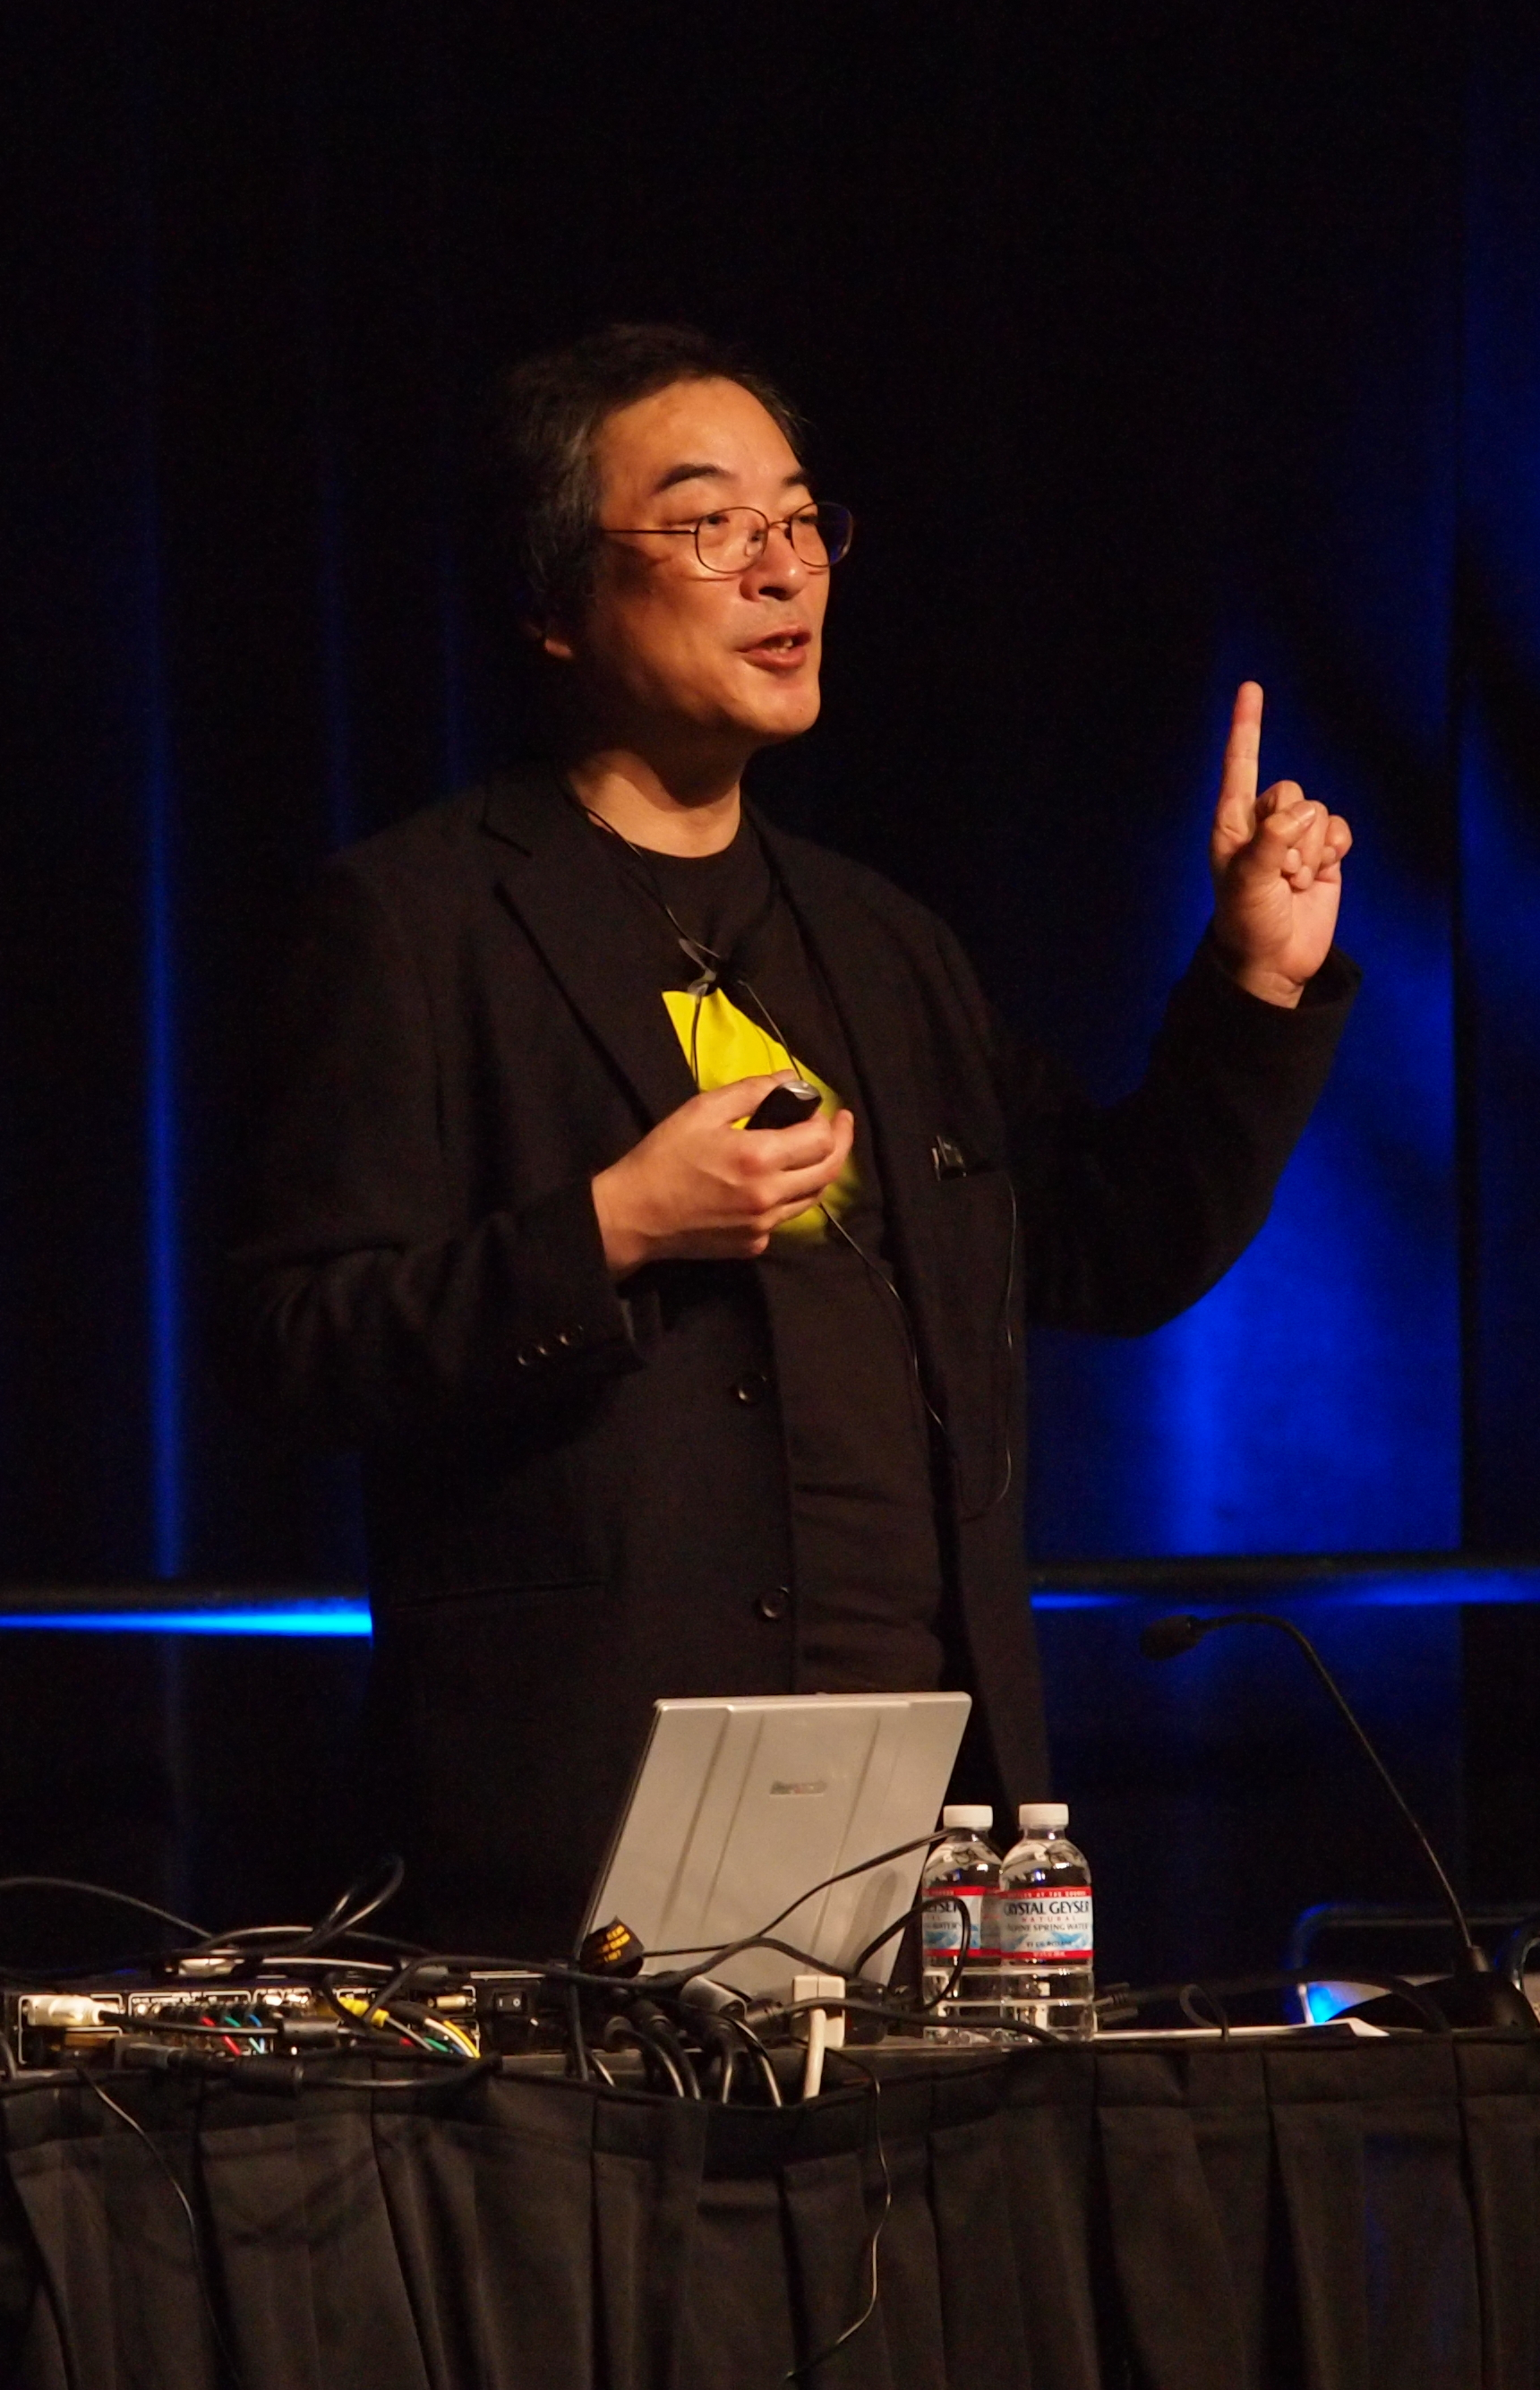
\includegraphics[width=0.4\textwidth]{img/imgConLicenza/toruIwatani/toruIwatani.jpg}
  \caption{Toru Iwatani, creatore di Pac-Man, alla GCD (Game Developers Conference) nel 2011.}
  \label{toruIwatani}
\end{wrapfigure}

Gli agenti del \emph{ghost team} sono implementati in un modulo dedicato. Ogni fantasma ha una funzione specifica che rappresenta il suo agent. Quindi, ciascun agent viene attivato dal controller chiamando la sua funzione. Queste sono:

\texttt{
\begin{itemize}
\item
  gioca\_blinky
\item
  gioca\_pinky
\item
  gioca\_inky
\item
  gioca\_clyde
\end{itemize}
}

Prima di entrare nei dettagli dei singoli agenti, leggiamo questa frase del creatore di Pac-Man, che ci fa capire perché ogni fantasma ha bisogno di un agent personalizzato:\\

\tcbset{width=0.9\textwidth,boxrule=0pt,colback=BoxColor,arc=0pt,auto outer arc,left=0pt,right=0pt,boxsep=5pt}

\begin{tcolorbox}
``To bring some tension into the game, I wanted the monsters to surround Pac-Man at a certain stage of the game. But I felt that it would create stress for the player if he were constantly surrounded by ghosts. Therefore, I had the monsters surround him in waves: first attack, then retreat. When they regrouped, the attack began again. It seemed to me more natural than a constant attack. ''\\
  - Toru Iwatani, creator of Pac-Man
\end{tcolorbox}

\tcbset{width=1\textwidth,boxrule=0pt,colback=CremeColor,arc=0pt,auto outer arc,left=0pt,right=0pt,boxsep=5pt}

Toru Iwatani, ci svela quindi che le personalità del ghost team, non nascono né a caso né per pure esigenze algoritmiche, ma per creare la giusta tensione nella mente del giocatore!

\textbf{Blinky} , il fantasma rosso, punta direttamente alla cella di Tuki. I suoi cambi di direzione sono stabiliti solo quando attraversa un incrocio e inoltre, durante la sua caccia, non gli è permesso invertire la direzione del movimento. La strategia di Blinky lo porta ad essere il più aggressivo e temuto dei quattro.

\textbf{Pinky} , quello rosa, punta alla cella che si trova quattro posizioni davanti a Pac-Man. Come già specificato per Blinky, anche per Pinky e per gli altri fantasmi si applica il principio secondo cui il cambio di direzione viene preso solo in corrispondenza ad un incrocio e, per questo principio, non è escluso che Pinky catturi Pac-Man anche se punta di fronte a lui e non direttamente alla sua cella.

\textbf{Inky} , il fantasma blu, ha un comportamento più complesso da prevedere rispetto ai due appena visti, infatti la sua cella bersaglio non dipende solo dalla posizione di Pac-Man ma anche dalla posizione di Blinky. Inky sceglie infatti di orientarsi verso la cella intermedia tra i due.

Il comportamento di \textbf{Clyde} è un po' confuso. Inizialmente insegue Pac-Man usando la stessa strategia di Blinky, ma quando si avvicina troppo (8 celle) cambia ed entra in modalità \emph{diffusione}, girovagando intorno ad una cella prestabilita che non è quella di Pac-Man. In questo modo Clyde aiuta a catturare Pac-Man, ma non si espone mai troppo.

\textbf{N.B.} La nostra implementazione degli agenti dei fantasmi si basa sulla rappresentazione del labirinto come un grafo, che è l'obiettivo principale di questo libro. Alla fine di questo libro sarete in grado di analizzare il codice di detti agenti e modificarlo a piacere.

\newpage
\section{L'agent di Pac-Man}

L'agent di Pac-Man è implementato nella funzione gioca\_tuki. Tutta la logica dell'agent deve pertanto essere implementata nella seguente funzione:\\

\textbf{Listato} \texttt{gioca\_tuki\_vuoto.c} \\


  \begin{spacing}{0.9}
    \begin{small}
      \begin{tcolorbox}
\begin{verbatim}
#include "tuki5_modello.h"
#include <stdio.h>
#include <unistd.h>

direzione gioca_tuki (posizioni posi, oggetto ** labx)
{
  direzione static ld = SINISTRA; 
  return ld;
}
\end{verbatim}
\end{tcolorbox}
    \end{small}
  \end{spacing}


il parametro di input posi è una struttura che contiene le coordinate di tutti i personaggi (Pac-Man stesso e i fantasmi):


  \begin{spacing}{0.9}
    \begin{small}
      \begin{tcolorbox}
\begin{verbatim}
  typedef struct  {
  int tuki_x, tuki_y;
  int blinky_x, blinky_y;
  int inky_x, inky_y;
  int pinky_x, pinky_y;
  int clyde_x, clyde_y;
} posizioni;
\end{verbatim}
\end{tcolorbox}
    \end{small}
  \end{spacing}


Tutti i nomi dei membri della struttura sono autoesplicativi tranne \texttt{tuki\_x} e \texttt{tuky\_y}. Il nome Tuki viene utilizzato in tutto il codice anziché Pac-Man, poiché Tuki e Giuli sono le mascottes di tutti i nostri progetti e di tutte le nostre pubblicazioni. Per questo, nella versione del nostro gioco, spesso scriviamo che il protagonista è Tuki e non Pac-Man.\\
Il parametro \texttt{labx} è una copia dell'array usato per rappresentare il labirinto e può essere utilizzato dall'agent per scegliere la direzione da prendere.\\
Il parametro di output \texttt{ld} restituisce al controller la direzione del movimento scelta dall'agent, dove direzione è un tipo definito come:


  \begin{spacing}{0.9}
    \begin{small}
      \begin{tcolorbox}
\begin{verbatim}
typedef enum {SINISTRA, SU, DESTRA, GIU, FERMO} direzione;
\end{verbatim}
\end{tcolorbox}
    \end{small}
  \end{spacing}


Per vincere la partita, l'agent Pac-Man deve 1) scappare dai fantasmi e 2) mangiare tutte le pillole nel labirinto. Questi obiettivi devono essere implementati nella funzione \texttt{gioca\_tuki}. Questo libro ha lo scopo di presentare alcuni fondamenti della teoria dei grafi per raggiungere questi obiettivi.


\section{Cosa è un grafo?}

I grafi vengono utilizzati per modellare le relazioni tra coppie di oggetti. Ad esempio, data una serie di punti nel piano cartesiano, la distanza cartesiana tra loro può essere rappresentata con un grafo. È molto importante notare che lo stesso grafo può rappresentare molte distribuzioni diverse di punti, poiché la distanza tra i punti viene preservata ruotando l'insieme di punti nel piano.\\
Un famoso esempio è lo Zachary Karate Club \cite{Zachary} in cui viene utilizzato un grafo per rappresentare le relazioni tra le coppie dei membri del club. I vertici corrispondono ai membri e gli archi che collegano due vertici rappresentano la relazione tra due membri del club.\\

\textsc{Take home message:} I grafi non hanno un singolo campo di applicazione, ma possono essere usati in campi diversi per rappresentare le relazioni che possono esservi definite.


\part{Pac-Man agent limitato alla Partial Observability}

\chapter{Pac-Man vaga nel labirinto}

Per iniziare la nostra analisi, semplifichiamo il contesto del gioco e facciamo finta che:

\begin{enumerate}
\item
  non ci siano fantasmi a caccia di Pac-Man dentro al labirinto
\item
  Pac-Man abbia una Partial Observability (PO) del labirinto.
\end{enumerate}

Secondo Williams \cite{Williams} ``PO è la compromissione della capacità di un agent di osservare completamente il mondo in cui si trova'', un'idea semplice di PO è data dalle due immagini sottostanti.

\begin{figure}[H]
\centering
  
  \begin{subfigure}[b]{0.49\textwidth}
    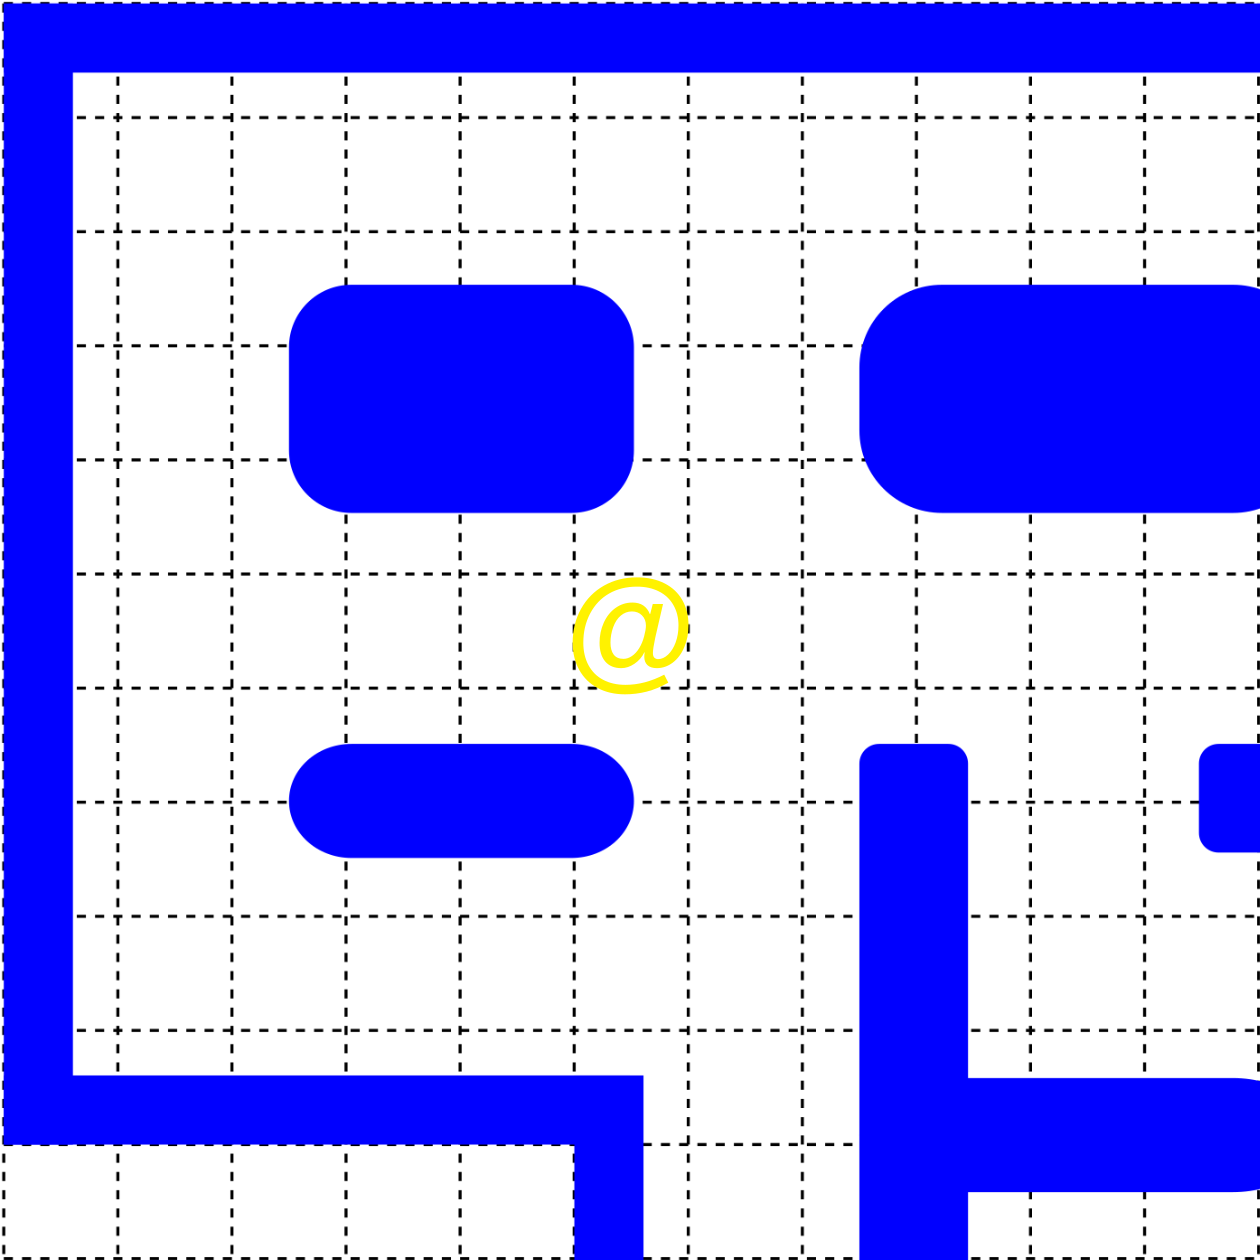
\includegraphics[width=\textwidth]{img/po_2.png}
    \caption{Osservabilità totale}
    \label{to}
   \end{subfigure}
  \begin{subfigure}[b]{0.49\textwidth}
    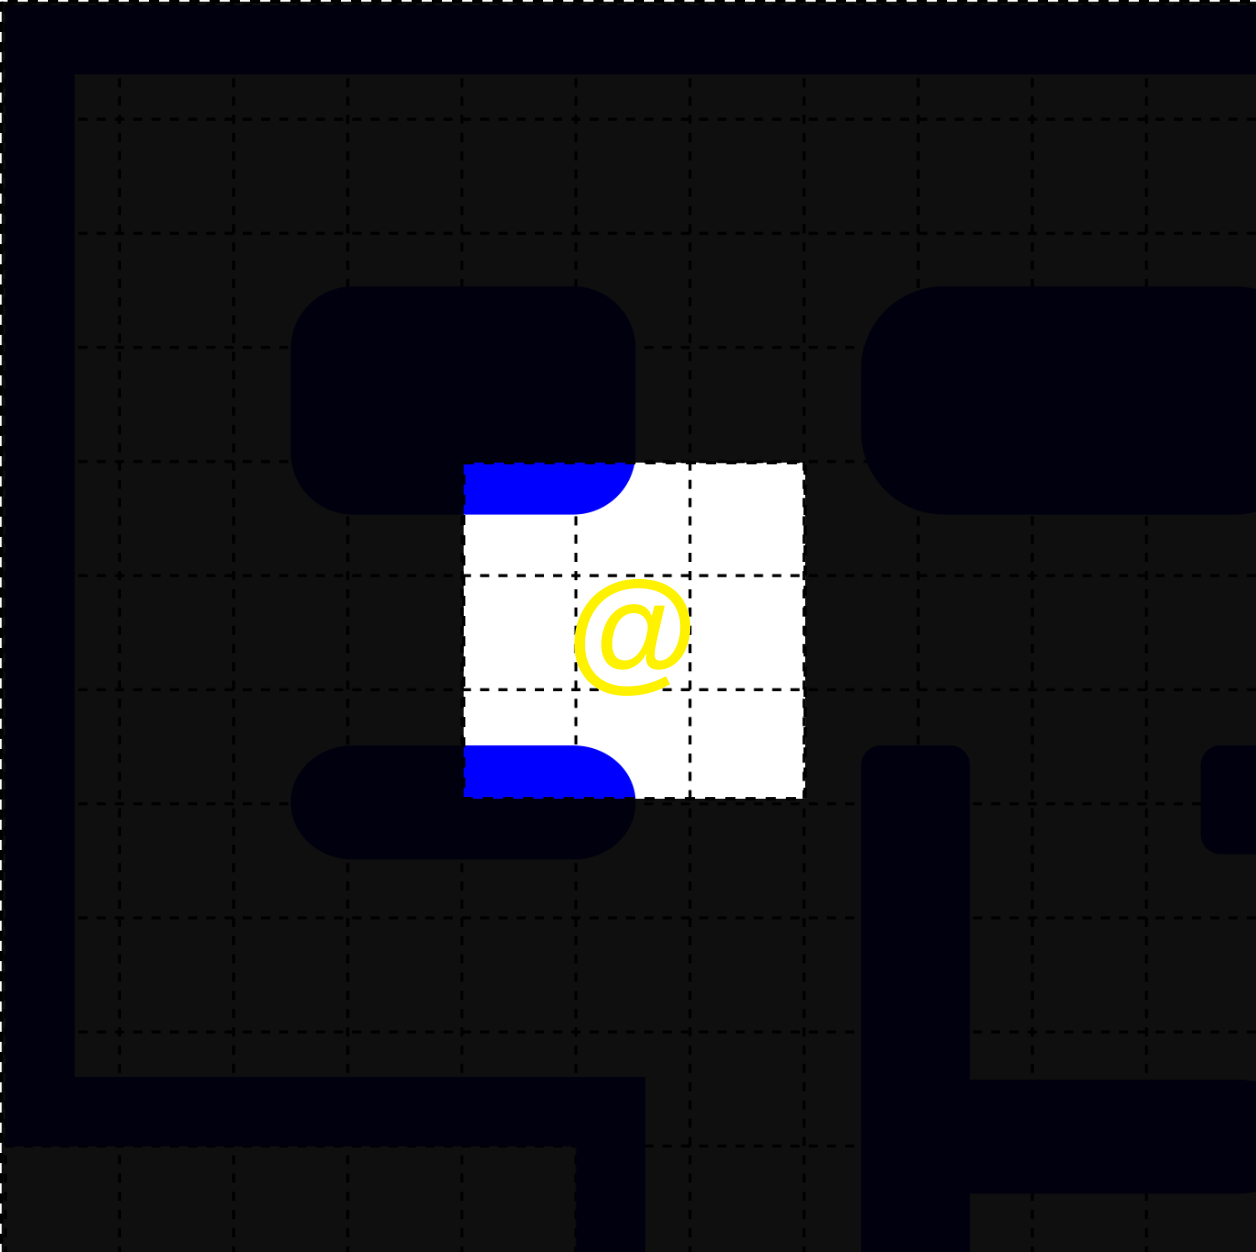
\includegraphics[width=\textwidth]{img/po_1.png}
    \caption{Osservabilità parziale}
    \label{po}
  \end{subfigure}

  \caption{La prima figura \ref{to} mostra l'agent Pac-Man con osservabilità totale del labirinto: cioè la stessa visione del giocatore umano. La seconda \ref{po} mostra l'agent Pac-Man con osservabilità parziale, metaforicamente analoga alla vista ottenuta vagando con una candela in un labirinto buio.
} 
\end{figure}

Ad ogni ciclo di gioco Pac-Man può osservare solo le celle adiacenti alla sua posizione corrente controllando se esse appartengono a dei corridoi, quindi sono accessibili, oppure alle pareti del labirinto e quindi sono ostacoli. Ogni cella del labirinto ha otto celle vicine.

\section{Le celle confinanti}

La riga e la colonna di Pac-Man all'interno del labirinto sono memorizzate nella struttura \texttt{posi}

  \begin{spacing}{0.9}
    \begin{small}
      \begin{tcolorbox}
\begin{verbatim}
int i = posi.tuki_y;
int j = posi.tuki_x;
\end{verbatim}
\end{tcolorbox}
    \end{small}
  \end{spacing}


\textsf{Ricorda: la struttura} \texttt{posi} \textsf{è un parametro passato alla funzione} \\\texttt{gioca\_tuki}.\\

La riga e la colonna di ognuna delle otto celle confinanti con quella di Pac-Man sono ottenute a partire dalle variabili indice $i$ e $j$ incrementandole o diminuendole di una unità, per un totale di $2^3$ diverse combinazioni (Vedi figura \ref{confinanti})

\begin{figure}
  \centering
  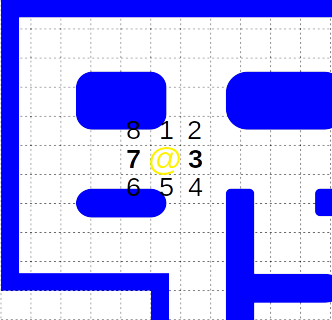
\includegraphics[width=0.6\textwidth]{img/labPac1.png}
  \caption{Le celle vicine (confinanti) a quella di Pac-Man sono numerate da 1 a 8. Solo le celle 3 e 7 sono accessibili, le celle 8 e 6 sono infatti occupate da elementi di muro, mentre la 2 e la 4 richiedono un movimento in diagonale che non è previsto in questo gioco.}
  \label{confinanti}
\end{figure}

Per stabilire la direzione in cui muoversi, l'agent deve conoscere la disposizione dei muri rispetto alla sua attuale posizione. L'agent può memorizzare il tipo di oggetti che lo circondano \emph{accedendo al labirinto} come segue: 


  \begin{spacing}{0.9}
    \begin{small}
      \begin{tcolorbox}
\begin{verbatim}
oggetto s,d,a,b;
oggetto sa,sb,da,db;
//Ortogonali
s = labx[i][j-1]; //Sinistra
d = labx[i][j+1]; //Destra
a = labx[i-1][j]; //Alto
b = labx[i+1][j]; //Basso
//Diagnonali
sa = labx[i-1][j-1]; 
sb = labx[i+1][j-1]; 
da = labx[i-1][j+1]; 
db = labx[i+1][j+1];
\end{verbatim}
\end{tcolorbox}
    \end{small}
  \end{spacing}


\textsf{Ricorda: l'array} \texttt{labx} \textsf{è anch'esso un parametro della funzione} \\\texttt{gioca\_tuki}.\\

\section{Algoritmo dell'agent di Pac-Man}

L'obiettivo di Pac-Man è di mangiare tutte le pillole distribuite lungo il campo di gioco. In questa prima fase abbiamo deciso di non considerare i fantasmi, quindi, per raggiungere il suo obiettivo, l'agent deve semplicemente attraversare in lungo e in largo tutti i corridoi a alla fine le pillole saranno esaurite.\\
In questa prima sezione vediamo come l'agent può percorrere tutto il labirinto, anche gli angoli nascosti, senza averne una visione dall'alto.\\
L'algoritmo che proponiamo si basa sulle regole seguenti:

\begin{enumerate}
\item
  non dirigerti contro i muri
\item
  scegli una direzione arbitraria (random) se la direzione attuale ti porta contro un muro
\item
  scegli una direzione casuale in corrispondenza di un incrocio
\item
  non cambiare direzione se non si verifica una delle condizioni precedenti.
\end{enumerate}

Il \texttt{model} della piattaforma impedisce che Pac-Man attraversi un muro del labirinto indipendentemente dalla direzione di movimento scelta dall'agent (per chi ha letto \emph{Sfidare gli algoritmi}, sempre degli stessi autori, si ricorda che il \texttt{model} implementa la fisica del campo di gioco). Comunque, se l'agent sceglie male la direzione e decide di dirigersi contro un muro del labirinto, come risultato avrà perso un ciclo di gioco. Da qui si spiega la regola 1) che ha come primo obiettivo quello di evitare questo spreco.\\
La regola 2) risponde all'esigenza di Pac-Man di mangiare tutte le pillole e quindi di percorrere tutti i corridoi in cui esse sono presenti. Quando Pac-Man incontra un ostacolo (muro) deve scegliere una nuova direzione. Dal momento che l'agent non ha conoscenza pregressa della struttura del labirinto, per massimizzare le probabilità di percorrere tutti i corridoi, dovrà appellarsi alla statistica, confidando che una scelta casuale della direzione lo porterà prima o poi a visitare tutti i corridoi del labirinto.\\
La regola 3) sceglie una direzione in modo probabilistico (random). Cambiare direzione solo quando si incontra un ostacolo non è sufficiente a garantire il completamento del percorso, ci sono infatti nel labirinto diversi incroci che si presentano anche in corrispondenza di un cammino accessibile e non interrotto. Per questo è necessario che l'agent valuti la possibilità di cambiare direzione anche se non incontra un ostacolo.\\
La regola 4) infine impedisce a Pac-Man dei cambi di direzione immotivati. Questo aumenta la possibilità di percorre il labirinto in tempi brevi ed evita l'effetto ``ping-pong'' che darebbe anche visivamente un senso di incertezza.\\

\textsf{La condizione di PO è stata implementata nel codice che segue come già discusso poco sopra. Per implementare la regola 4), la variabile} \texttt{ld}, \textsf{che memorizza la direzione scelta dall'agent, è dichiarata come} \texttt{static} \textsf{in modo da poterne confrontare il valore nei successivi turni di gioco.}\\

\section{Limiti della soluzione implementata}

\begin{wrapfigure}{R}{0.5\textwidth}
  \centering
  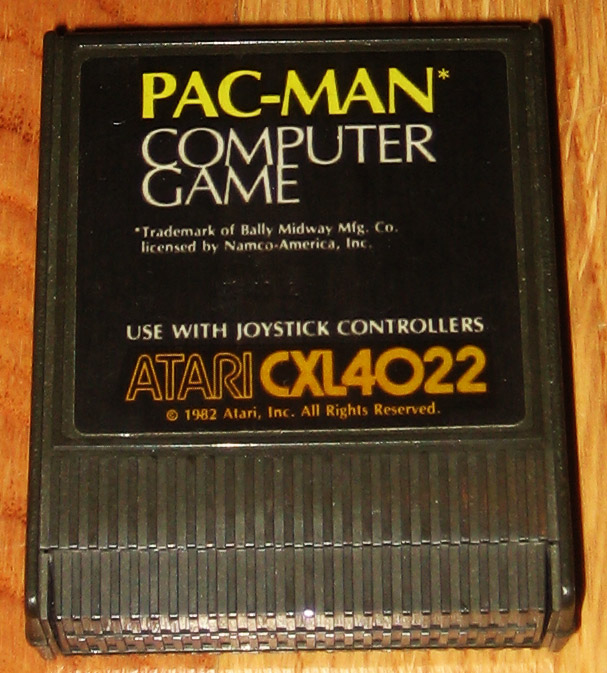
\includegraphics[width=0.5\textwidth]{img/imgConLicenza/cartuccia/cartuccia.jpg}
  \caption{Cartuccia di Pac-man, videogioco per computer Atari a 8 bit. Modello CXL4022. 1982.}
  \label{cartuccia}
\end{wrapfigure}

La soluzione implementata nel codice visto sopra è una soluzione \emph{state-less}, cioè, fatto salvo per la direzione scelta, non preserva lo stato di conoscenza acquisita dall'agent tra un turno di gioco e il successivo.\\
L'approccio state-less può essere una soluzione efficiente in alcune specifiche topologie di labirinto. Per esempio si consideri un labirinto alternativo a quello di Pac-Man costituito da un semplice otto, cioè due percorsi ciclici che si uniscono in un singolo incrocio.\\

È immediato realizzare che anche un algoritmo state-less può garantire il completamento di tale percorso in tempi certi. \`E infatti sufficiente impostare l'agent in modo che in caso di incrocio scelga (per esempio) la direzione destra e, in questo modo, all'incrocio tra i due anelli l'agent abbandona il primo e segue il secondo.\\

\texttt{ld = DESTRA;}\\
\newline
La stessa logica applicata al labirinto di Pac-Man lo porterebbe a girare ininterrottamente attorno ad una delle aiuole senza più completare il resto del percorso.\\

Prima di discutere come migliorare l'agent del Pac-Man, è il momento di provarne l'implementazione e vederla in pratica.


\section{Compilare il codice e lanciare l'eseguibile}

Iniziamo a vedere come compilare ed eseguire i sorgenti. Per questa prima prova implementiamo per Pac-Man un agent molto basilare che lo faccia rimanere fermo all'interno del labirinto.

Ci sono due modi per compilare il codice: 1) editare il listato, 2) scaricare o clonare il progetto da GitHub.\\
Per il modo 1):

\begin{enumerate}
\item
  Creare la struttura di directory seguente:

  \begin{itemize}
  \item
    grafi
  \item
    grafi/ghost\_team
  \item
    grafi/mvc
  \item
    grafi/PacMan
  \end{itemize}
\item
  creare un file nominato \texttt{grafi/compila.sh} con il codice seguente:\\

  \textbf{Listato} \texttt{compila.sh}

  \tcbset{width=0.9\textwidth,boxrule=0pt,colback=CremeColor,arc=0pt,auto outer arc,left=0pt,right=0pt,bottom=0pt,boxsep=5pt}
  
  \begin{spacing}{0.9}
    \begin{small}
        \begin{tcolorbox}
\begin{verbatim}
#!/bin/sh

if [ "$#" -ne 3 ]; then
    echo "3  parameters required:\n
    \tUser codice file (gioca_tuki.c for example)\n
    \t1 or 0 to activate or no run away option\n
    \tTime delay for each game cycles (ms)\n"
    exit
fi

gcc -pedantic -std=c99 -o tuki5.game -DFUGA=$2 
-DDELAY=$3 \
$1 \
ghost_team/gioca_fantasmi.c \
mvc/tuki5_controllo.c \
mvc/tuki5_modello.c \
mvc/tuki5_visore.c \
-Imvc \
-lm
\end{verbatim}
\end{tcolorbox}
      \end{small}
    \end{spacing}

  \tcbset{width=1\textwidth,boxrule=0pt,colback=CremeColor,arc=0pt,auto outer arc,left=0pt,right=0pt,bottom=0pt,boxsep=5pt}
  
\item
  Editare i file seguenti:

  \begin{itemize}
  \item
    \texttt{grafi/mvc/tuki5\_modello.h}
  \item
    \texttt{grafi/mvc/tuki5\_modello.c}
  \item
    \texttt{grafi/mvc/tuki5\_visore.h}
  \item
    \texttt{grafi/mvc/tuki5\_visore.c}
  \item
    \texttt{grafi/ghost-team/gioca\_fantasmi.c}
  \item
    \texttt{grafi/PacMan/gioca\_tuki\_vuoto.c}
  \end{itemize}
\item
  Cambiare la directory in grafi e lanciare \texttt{compila.sh}:

  \begin{itemize}
  \item
    \texttt{\textasciitilde{}\textbackslash{}\$ cd grafi}
  \item
    \texttt{\textasciitilde{}/grafi\textbackslash{}\$ chmod +x compila.sh}
  \item
    \texttt{\textasciitilde{}/grafi\textbackslash{}\$ ./compila.sh PacMan/gioca\_tuki\_vuoto.c\\0 100}
  \end{itemize}
  
  I tre parametri passati allo script (\texttt{compila.sh}) sono: il file utente con il codice dell'agent che si vuole integrare alla piattaforma, un booleano ($0$ o $1$) che determina se attivare l'opzione di fuga dell'agent dal ghost-team, il ritardo in millisecondi con cui viene mostrato ogni turno di gioco.
\item
  Imposta il terminale su almeno $50$ righe e $50$ colonne e avvia l'eseguibile \texttt{tuki5.game} per iniziare il gioco:

  \begin{itemize}
  \item
    \texttt{\textasciitilde{}/grafi\textbackslash{}\$ ./tuki5.game}
  \end{itemize}

  All'avvio del programma si deve vedere sul terminale lo stesso che è riportato in figura \ref{labTerminale}. Si ricordi però che il modulo \texttt{viewer} non modifica il colore di sfondo del monitor, quindi se si vuole che sia nero lo si setti dalle proprietà della finestra, o si setti qualsiasi altro colore compatibilmente con i colori che sono già stati usati nel gioco.

  Come si vedrà, Pac-Man rimane fermo al centro del labirinto mentre i fantasmi del ghost team lo circondano e lo bloccano (mangiano). Pac-Man non prova a fuggire né a muoversi perché il codice dell'agent che abbiamo inserito come input a \texttt{compila.sh} non ha logica di fuga né di esplorazione del labirinto.
\end{enumerate}

\begin{figure}
  \centering
  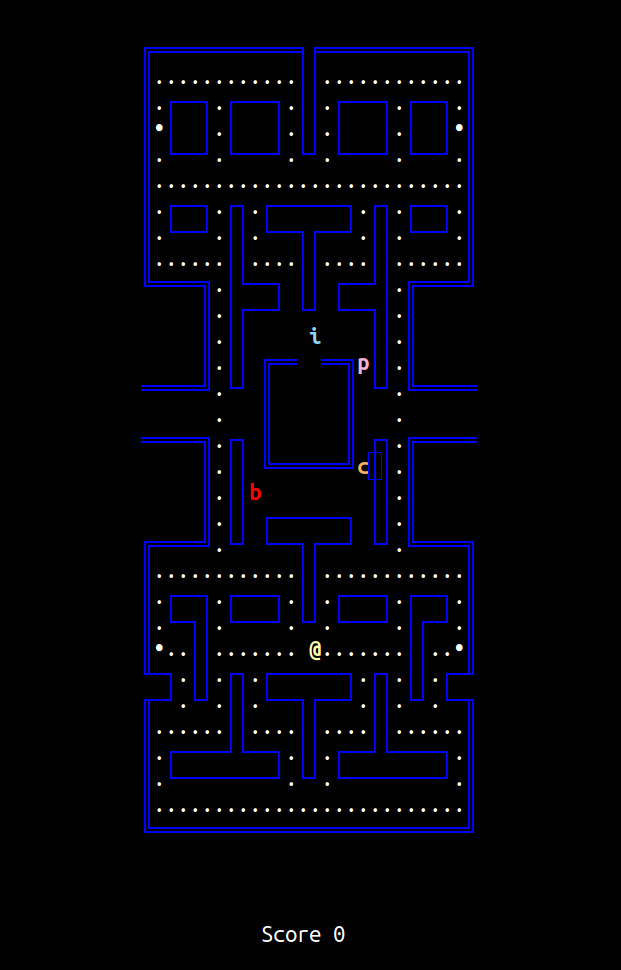
\includegraphics[width=0.9\textwidth]{img/tuki5_campo.jpg}
  \caption{Il labirinto di Pac-Man creato come una griglia di caratteri.}
  \label{labTerminale}
\end{figure}

\section{\texttt{gioca\_tuki\_random.c} in azione}

A questo punto si è capito lo scopo di ogni file della piattaforma e il ruolo dello \emph{user code} \texttt{gioca\_tuki\_(quello che vuoi).c}. Ora è il momento di provare il codice implementato nell'agent \texttt{random} e vedere cosa è capace di fare!\\
Si seguano le istruzioni seguenti:\\
\newline
\texttt{\textasciitilde{}/grafi\textbackslash{}\$ ./compila.sh PacMan/gioca\_tuki\_random.c\\ 0 50}\\
\texttt{\textasciitilde{}/grafi\textbackslash{}\$ ./tuki5.game}\\

Dopo l'avvio del programma Pac-Man inizia a vagare per il labirinto seguendo le quattro regole viste prima. Ai fantasmi occorrerà poco tempo per catturarlo perché non è stata attivata l'opzione di fuga.\\
Per vedere Pac-Man completare il labirinto specifichiamo che non ci devono essere fantasmi nel ghost team e lanciamo ancora l'esecuzione:\\
\newline
\texttt{\textasciitilde{}/grafi\textbackslash{}\$ ./tuki5.game 0}\\

Lo 0 indica il numero di fantasmi in azione.\\
A seconda del valore \texttt{DELAY} usato durante la compilazione, si dovranno aspettare un paio di minuti affinché Pac-Man finisca il labirinto. Guardando questa gara con zero fantasmi si potrà capire la personalità dell'agent codificato nel file sorgente e iniziare a pensare a come migliorarlo!\\
Il model non impedisce all'agent di entrare nella casa del ghost team, dove Pac-Man può anche essere catturato, specialmente se i quattro fantasmi sono all'interno. Se si preferisce impedire questa eventualità è necessario modificare il labirinto con il codice seguente:

  \begin{spacing}{0.9}
    \begin{small}
      \begin{tcolorbox}
\begin{verbatim}
labx[16][2]  = 'A';
labx[16][23] = 'A';
labx[14][13] = 'A';
labx[14][14] = 'A';
\end{verbatim}
\end{tcolorbox}
    \end{small}
  \end{spacing}


\subsection{La fuga di Pac-Man}

Fin'ora si è visto come implementare un semplice agent che, basandosi sulla eventualità probabilistica, ha ottime prospettive di completare il labirinto, però come si è potuto verificare la sua esplorazione ha vita breve se si abilitano uno o più fantasmi del ghost team.

Analizzando il codice \texttt{gioca\_tuki\_random.c} si vede però che è stata implementata una logica che permette a Pac-Man di evitare gli attacchi diretti dei fantasmi.

In pratica viene verificato che le coordinate di ogni fantasma (ciclo for da 1 a 4) non siano adiacenti a quelle di Pac-Man e, in questo caso, viene impostato a 1 il flag di prossimità che permette all'agent di cambiare direzione rispetto a quella di cattura.

Per provare la modalità fuga, si compili impostando ad 1 il flag di fuga (vedi sopra) e si lanci l'eseguibile specificando 1 come numero di fantasmi.\\
\newline
\texttt{\textasciitilde{}/grafi\textbackslash{}\$ ./tuki5.game 1}

  \begin{spacing}{0.9}
    \begin{small}
      \begin{tcolorbox}
\begin{verbatim}
int x = posi.tuki_x;
int y = posi.tuki_y;
int x_g[4];
int y_g[4];
...
char s_g = 0, d_g = 0,a_g = 0,b_g = 0;
for (int ig = 0; ig<4; ig++)
  {
    s_g = s_g || ( x_g[ig] < x) &&
      ( x - x_g[ig] <=2 )  && (y == y_g[ig]); 
    s_g = s_g || ((x_g[ig] == x-1) &&
                  (y_g[ig] == y+1));
    s_g = s_g || ((x_g[ig] == x-1) &&
                  (y_g[ig] == y-1));
    d_g = d_g || ( x_g[ig] > x) &&
      (x_g[ig] - x <= 2) && (y == y_g[ig]);
    d_g = d_g || ((x_g[ig] == x+1) &&
                  (y_g[ig] == y+1));
    d_g = d_g || ((x_g[ig] == x+1) &&
                  (y_g[ig] == y-1));
    a_g = a_g || (x == x_g[ig]) &&
      ( y >  y_g[ig]) && ( y - y_g[ig] <=2);
    a_g = a_g || ((y == y_g[ig] + 1) &&
                  (x_g[ig] == x+1));
    a_g = a_g || ((y == y_g[ig] + 1) &&
                  (x_g[ig] == x-1));
    b_g = b_g || (x == x_g[ig]) &&
      ( y <  y_g[ig]) && ( y_g[ig]- y <=2);
    b_g = b_g || ((y == y_g[ig] - 1) &&
                  (x_g[ig] == x+1));
    b_g = b_g || ((y == y_g[ig] - 1) &&
                  (x_g[ig] == x-1));
  }
...
if((s_g || d_g || a_g || b_g) && FUGA)
  {
    ...
  }
\end{verbatim}
    \end{tcolorbox}
  \end{small}
\end{spacing}

\newpage
\section*{Box domande n.1}
\addcontentsline{toc}{section}{Box domande n.1}

\begin{enumerate}
\item Cos'è la Partial Observability?
\begin{enumerate}
\def\labelenumi{\alph{enumi}.}
\item
  L'incapacità dell'agent di vedere oltre le celle a lui immediatamente adiacenti
\item
  L'incapacità dell'agent di vedere in diagonale
\item
  La possibilità andare in una sola direzione
\end{enumerate}

\item Se un fantasma è a due celle di distanza dal Pac-Man e Pac-Man è guidato dall'agent \emph{random}, Pac-Man cambia direzione?

\begin{enumerate}
\def\labelenumi{\alph{enumi}.}
\item
  Sì, perché l'agent random tende a far stare il Pac-Man a distanza di sicurezza dai fantasmi
\item
  No, perché l'algoritmo di fuga prevede un avvicinamento al fantasma prima di scappare
\item
  No, perché la partial observability gli impedisce di vedere a due celle di distanza
\end{enumerate}

\item Esiste la possibilità che il Pac-Man, guidato dall'agent \emph{random}, non completi mai il labirinto?

\begin{enumerate}
\def\labelenumi{\alph{enumi}.}
\item
  Sì, la statistica ci dice che in un tempo infinito il completamento è certo, ma nel contesto di un'esecuzione che avviene in un tempo limitato, può sempre succedere
\item
  Sì, perché si tratta di un moto aleatorio
\item
  No
\end{enumerate}
\end{enumerate}


\chapter[Attraversamento deterministico]{Pac-Man attraversa in modo deterministico tutto il labirinto}

Nei paragrafi precedenti abbiamo visto come l'agent sia capace di completare il labirinto e mangiare tutte le pillole, basandosi solo sulla teoria delle probabilità o, in parole più semplici, scegliendo a caso dove svoltare ad ogni incrocio.\\
In molte situazioni questo approccio non è la soluzione ottimale, anche per le seguenti ragioni:

\begin{itemize}
\item
  il metodo probabilistico d\`a risultati garantiti solo in un tempo virtualmente infinito
\item
  anche nel caso che l'agent completi il labirinto potrebbe impiegarci un tempo inutilmente lungo.
\end{itemize}

Si immagini di lavorare in un'agenzia spaziale e di inviare un rover su Marte per esplorare l'intero territorio di una regione specifica e restituire alcuni dati di interesse. Sarebbe logico implementare l'algoritmo di \emph{vagabondaggio} probabilistico come agent del rover?\\
Probabilmente no, meglio continuare l'analisi e scoprire algoritmi più efficienti.

La pianificazione della \emph{copertura} completa di ambienti parzialmente noti o completamente sconosciuti è un problema comune nelle applicazioni di robotica anche sulla Terra, ad esempio per l'agricoltura assistita robotizzata. È un dato di fatto che questo tipo di attività è diventata molto comune con l'avvento dei robot mobili e dei micro-aerei (droni). Ad esempio, ci sono robot mobili che devono tagliare l'erba di un campo evitando di rovinare le aiuole dei fiori o di altre piante ornamentali, mentre per quel che riguarda i droni, questi devono definire delle \emph{no flight zones} per evitare ostacoli come alberi o edifici.\\
Per ora quindi, lascia che Marte ci aspetti e proseguiamo con l'analisi degli algoritmi.

\section{Decomposizione cellulare}

In questa sezione presenteremo il metodo detto \emph{boustrophedon}. Questo è un algoritmo specifico per eseguire una \emph{decomposizione cellulare} di un'\emph{area di lavoro}.

Con il termine area di lavoro si intende l'ambiente, la zona o lo spazio in cui l'agent deve agire. Nel caso di robot reali, l'area di lavoro potrebbe essere un giardino un cui tagliare l'erba, mentre per i droni potrebbe essere lo spazio sopra una città o tra i palazzi. Nel caso del Pac-Man sarà il suo labirinto.

Questo algoritmo è ampiamente utilizzato nelle odierne applicazioni di pianificazione di percorsi robotizzati \cite{Bahnemann}.

La sfida principale nella pianificazione automatica della copertura di un ambiente è la gestione degli ostacoli.

Con copertura si intende l'esplorazione completa dell'ambiente.

Per essere indipendente, l'agent di un robot dovrebbe essere in grado di identificare un percorso che lo conduca da un punto iniziale a un punto finale evitando collisioni.\\
Matematicamente, il problema può essere rappresentato come segue:

\begin{itemize}
\item
  Sia $A$ un robot che si sposta in un'area di lavoro $W$ e sia $W$ un sottoinsieme di $R^2$
\item
  $W$ è partizionato in regioni $C_{libera}$ e $C_{ostacolo}$, che sono rispettivamente regioni disponibili e non disponibili
\item
  dato un punto iniziale e un punto finale, l'obiettivo è quello di trovare un percorso che li colleghi e che si trovi completamente sulla regione $C_{libera}$.
\end{itemize}

Esistono diversi metodi che possono risolvere questo problema, qui ci concentreremo sulla decomposizione cellulare.

Dato un ambiente, il metodo di decomposizione cellulare è il primo passo per raggiungere la pianificazione e la copertura del percorso. Si compone di due passaggi:

\begin{enumerate}
\item
  Dividere l'ambiente in celle
\item
  Trasformare l'ambiente in un grafo in cui i vertici sono le celle e gli archi collegano i vertici corrispondenti alle celle adiacenti
\end{enumerate}

Nelle applicazioni della vita reale, il passaggio $1$ può essere una vera sfida da realizzare, per fortuna il labirinto Pac-Man è già composto da celle uniformi, quindi questo passaggio risulterà più semplice.

La decomposizione cellulare divide $C_{libera}$ in un insieme finito di regioni (celle) in modo tale che:

\begin{enumerate}
\item
  è triviale calcolare un percorso privo di collisioni tra due punti della stessa cella
\item
  è facile scoprire i vicini di ogni cella per costruire la roadmap (percorso)
\item
  è possibile determinare per ogni punto quale sia la cella che lo contiene
\end{enumerate}

Nella figura \ref{cellDec_siDec} mostriamo l'esatta decomposizione cellulare di uno spazio di lavoro mostrato nella figura \ref{cellDec_nonDec}. L'area verde (grigio chiaro) rappresenta $C_{libera}$, mentre i due poligoni arancioni (grigio scuro) sono gli ostacoli.

\begin{figure}
  \centering
  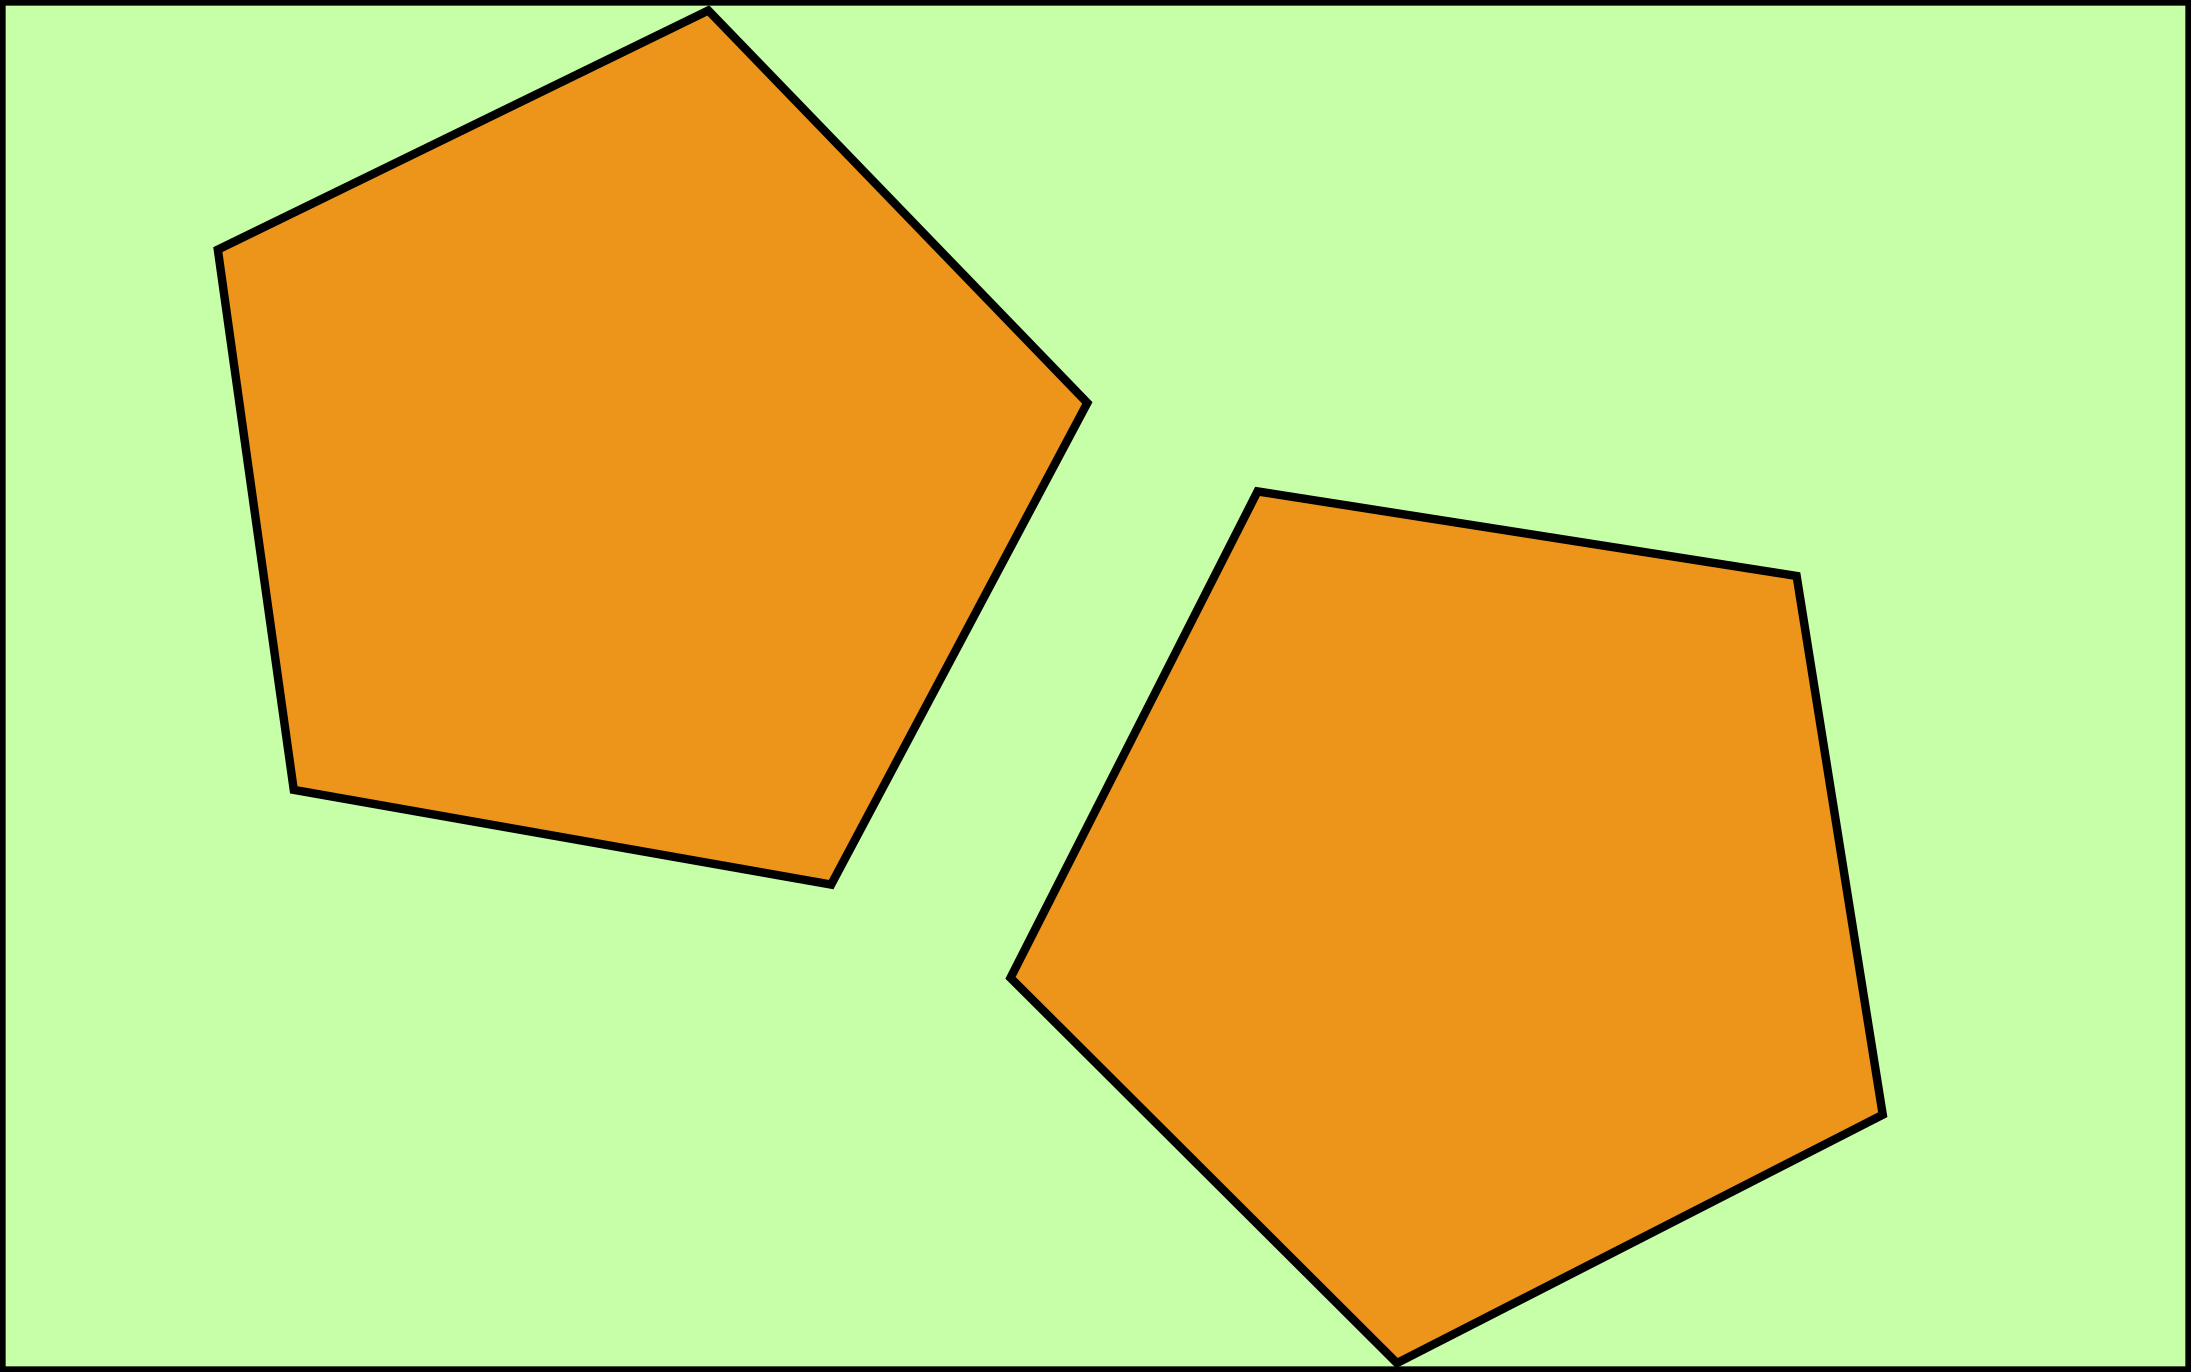
\includegraphics[width=0.6\textwidth]{img/cellDec_nonDec.png}
  \caption{Un esempio di un ambiente diviso in regioni accessibili (verde o grigio chiaro) e inaccessibili (arancione o grigio scuro).}
\label{cellDec_nonDec}
\end{figure}

\begin{figure}
  \centering
  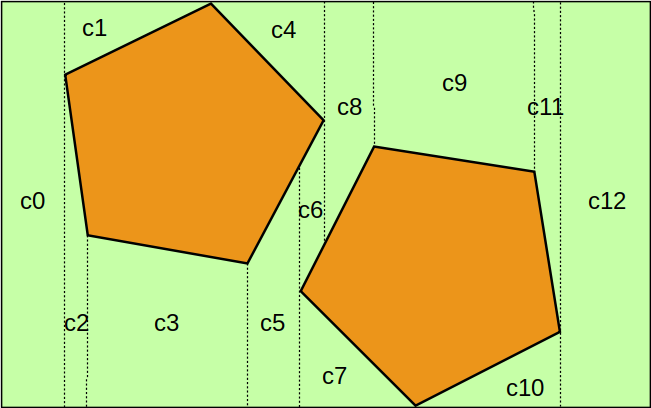
\includegraphics[width=0.6\textwidth]{img/cellDec_siDec.png}
  \caption{L'ambiente dopo la decomposizione cellulare.}
  \label{cellDec_siDec}
\end{figure}

Una volta effettuata la decomposizione delle celle, è possibile mappare $C_{libera}$ in un grafo (\ref{cellDec_grafo}) in cui:

\begin{itemize}
\item
  ogni cella è un vertice
\item
  i vertici corrispondenti alle celle adiacenti sono collegati da un bordo.
\end{itemize}

Una volta che lo spazio di lavoro è stato mappato su un grafo, il problema di coprire tutte le celle accessibili diventa un \emph{problema di grafi} (a graph problem) che può potenzialmente essere risolto con algoritmi su grafi esistenti.

\begin{figure}
  \centering
  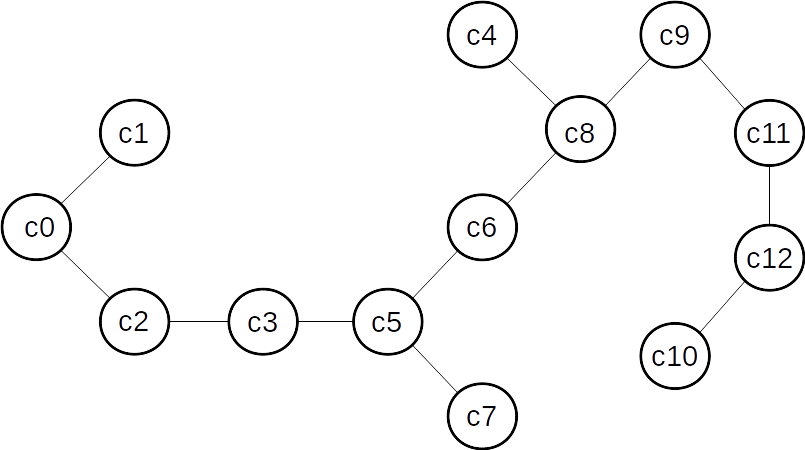
\includegraphics[width=0.6\textwidth]{img/cellDec_grafo.jpg}
    \caption{Il grafo creato dopo la decomposizione cellulare dell'area di lavoro.}
  \label{cellDec_grafo}
\end{figure}

\textsc{Take home message:}  Lo spazio di lavoro può essere mappato in un grafo in modo che l' \emph{attività di copertura} venga trasformata in algoritmi sui grafi.

\section{Algoritmo Boustrophedon}
L'algoritmo è stato descritto la prima volta da Choset \cite{Choset}. L'idea è di iniziare il percorso da una cella detta appunto cella iniziale per poi continuare a spostarsi da una cella all'altra in una determinata direzione che verrà chiamata direzione preferenziale.\\
La direzione intrapresa ad ogni passaggio di cella viene aggiunta a un elenco di passaggi che verranno utilizzati quando verrà rilevato un vicolo cieco nell'area di lavoro. Ogni cella in cui entra l'agent viene contrassegnata come visitata.\\
L'agent continua a spostarsi nella direzione preferenziale fino a quando non incontra un ostacolo. In tale situazione, controlla l'accessibilità di una cella vicina diversa dal suo obiettivo. Questo viene fatto cambiando direzione e cercando di fare un passo avanti. Se viene trovata una direzione accessibile, l'agent fa il passo in quella direzione quindi l'esecuzione dell'algoritmo continua come definito sopra. Al contrario, se l'agent incontra il vicolo cieco e quindi non è disponibile alcuna cella adiacente, fa un passo indietro e controlla le celle accessibili che lo circondano e che non siano già state visitate.\\ \par

Nella figura sotto abbiamo disegnato un labirinto semplificato ritagliato dal labirinto originale. Pac-Man cammina attraverso il  perimetro rettangolare maggiore evitando di prendere il primo incrocio sulla destra (linea verde o grigio chiaro). Quando raggiunge la posizione iniziale, scopre che non ci sono più celle non visitate intorno a lui, quindi torna indietro (linea rossa o grigio scuro) fino a raggiungere l'intersezione e prende la direzione che non aveva preso la prima volta (linea verde o grigio chiaro).\\

\begin{figure}
  \centering
  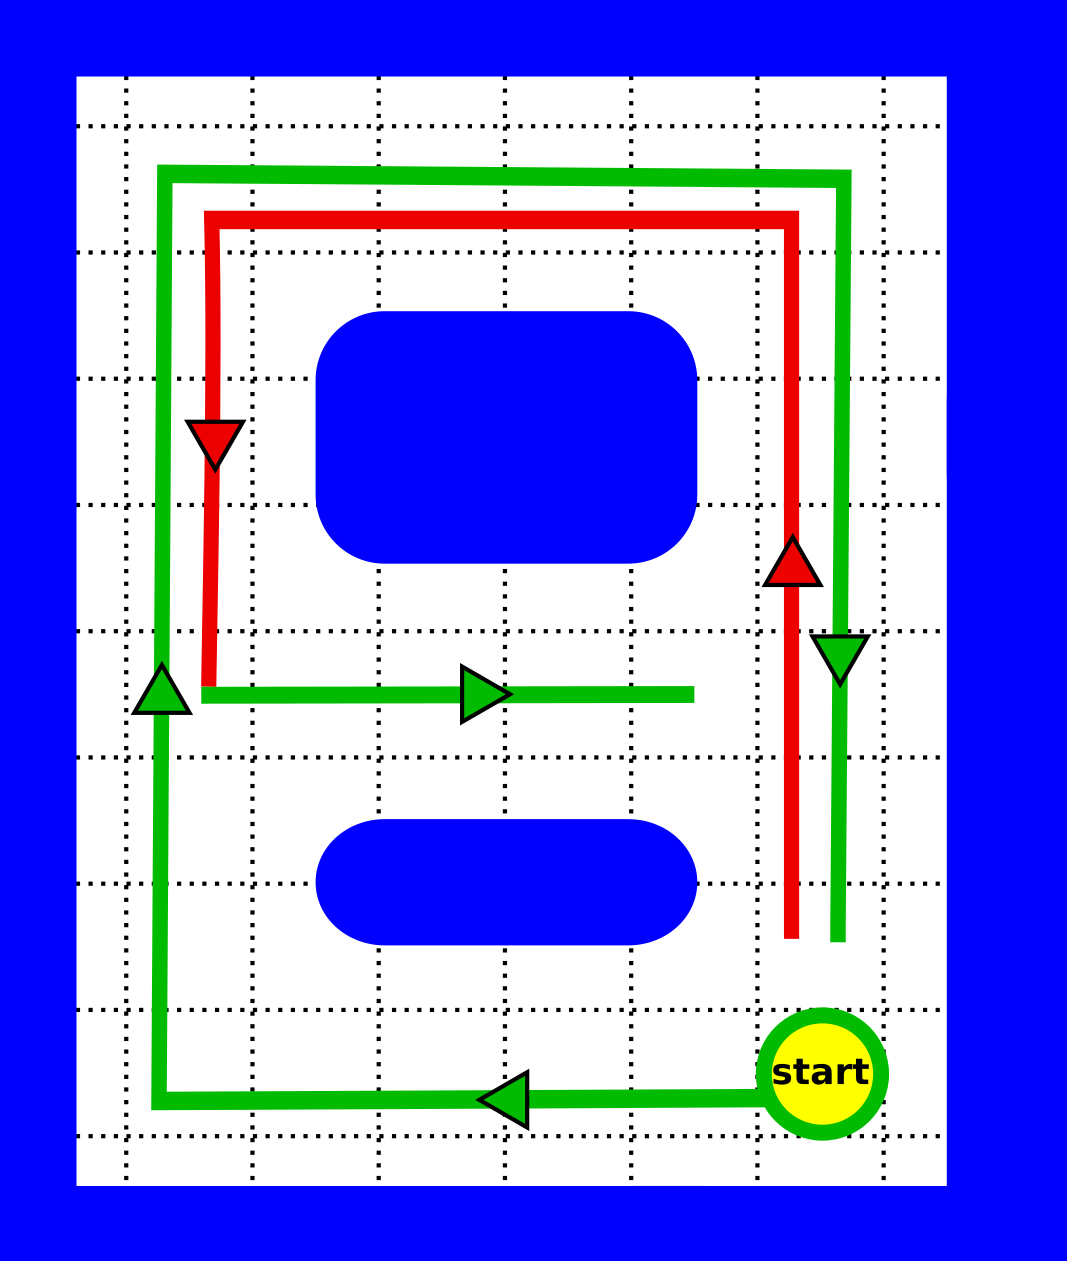
\includegraphics[width=0.6\textwidth]{img/pathBoustr.png}
    \caption{Pac-Man torna indietro quando non trova più celle disponibili.}
  \label{pathBoustr}
\end{figure}

\subsection{Strutture dati}
Per rappresentare ogni cella nel labirinto di Pac-Man useremo il tipo \texttt{struct} \texttt{agri\_Cella} definito come di seguito.\\

Ricorda di leggere l'appendice per comprendere il significato dei nomi e dei verbi latini.\\

  \begin{spacing}{0.9}
    \begin{small}
      \begin{tcolorbox}
\begin{verbatim}
typedef struct cella {
  Attributi d;
  struct cella* dextra;  
  struct cella* deorsum; //Giu
  struct cella* sinistra;
  struct cella* sursum;  //Su
} agri_Cella;
\end{verbatim}
    \end{tcolorbox}
  \end{small}
\end{spacing}

La struttura contiene quattro campi che sono dei puntatori alle quattro \texttt{agri\_Cella} sue vicine, e  un campo che descrive i suoi attributi definiti nella seguente struttura:

  \begin{spacing}{0.9}
    \begin{small}
      \begin{tcolorbox}
\begin{verbatim}
typedef struct dato
{
  int visitata;
  rei_genus rei;
} Attributi;
\end{verbatim}
    \end{tcolorbox}
  \end{small}
\end{spacing}

L'attributo \texttt{visitata} è $0$ se la cella è stata rilevata durante il cammino ma non visitata, mentre è $1$ se  la cella è stata anche visitata. Si noti che, se la cella non è stata rilevata, allora non esiste ancora nel grafo dell'agent.\\
L'attributo \texttt{rei\_genus} può essere "muro" o "qualcos'altro" e indica cosa contiene la cella.\\

\textsc{Take home message:}  ogni cella può essere pensata come un vertice di un grafo in cui i bordi sono le connessioni tra le celle.

\subsection{Connessione tra i vertici del grafo}\label{tocux5f30}

Nell'ultimo \emph{take home message}, abbiamo realizzato che le celle del labirinto sono come i vertici di un grafo. Tali vertici vengono scoperti durante l'esplorazione dell'agent e devono essere collegati tra loro. Questo compito viene implementato facendo in modo che le due celle (cella di Pac-Man e cella scoperta) puntino l'una verso l'altra nella direzione in cui è stata trovata la cella. Questo viene fatto usando la seguente funzione:

  \begin{spacing}{0.9}
    \begin{small}
      \begin{tcolorbox}
\begin{verbatim}
agri_Tabella agri_addo_Tabellam(
	     agri_Tabella tabella,Attributi d,versus dir)
{
  agri_Cella* n=(agri_Cella*)malloc(sizeof(agri_Cella));
  n->d=d;
  
  switch(dir)
    {
    case DEORSUM:
      tabella->sursum=n;
      n->deorsum=tabella;
      break;
    case SURSUM:
      tabella->deorsum=n;
      n->sursum=tabella;
      break;
    case DX:
      tabella->dextra=n;
      n->sinistra=tabella;
      break;
    case SX:
      tabella->sinistra=n;
      n->dextra=tabella;
      break;
    }
  return n;
}
\end{verbatim}
    \end{tcolorbox}
  \end{small}
\end{spacing}

dove \texttt{agri\_Tabella} è definito come: \\\texttt{typedef agri\_Cella* agri\_Tabella;}

Come si può notare, questo tipo di grafo è una sorta di tabella, infatti ogni vertice ha esattamente quattro spigoli.\\
L'idea di base è quella di utilizzare questa rappresentazione del grafo per creare l'algoritmo boustrophedon che consente a Pac-Man di attraversare il labirinto mantenendo una mappa costantemente aggiornata.

\subsection{Spostamento verso la cella successiva}\label{tocux5f31}

Ad ogni passo, Pac-Man collega fino a quattro vertici alla sua cella facendo crescere il grafo. Una volta che Pac-Man ha collegato tutte le celle vicine alla sua, deve decidere la cella successiva in cui spostarsi (cella bersaglio). Partendo da sinistra (la direzione preferenziale), l'agent controlla le altre tre direzioni, in ordine: su, destra e giù, fino a quando non trova una cella che non sia stata visitata e che non sia occupata da un muro.

  \begin{spacing}{0.9}
    \begin{small}
      \begin{tcolorbox}
\begin{verbatim}
 static agri_Tabella g=NULL;
...
 if(g->sinistra->d.visitata == 0
    && g->sinistra->d.rei != MURO) 
   {
     g=g->sinistra;
     g->d.visitata=1;
     agri_addo_Iter(&p,g);
     l=p;
     return SINISTRA;
   }
\end{verbatim}
    \end{tcolorbox}
  \end{small}
\end{spacing}

Se alla fine l'agent non ha trovato una cella disponibile, inizia a camminare all'indietro per trovare una cella che presenti almeno un incrocio inesplorato.

  \begin{spacing}{0.9}
    \begin{small}
      \begin{tcolorbox}
\begin{verbatim}
 /* Retraces his steps */

  l=l->prev;
  if(l==NULL) exit(-1);
  
  agri_addo_Iter(&p,l->locus);
  
  direzione nd;

  if(g->dextra==l->locus) nd=DESTRA; //Right
  else
  if(g->sinistra==l->locus) nd=SINISTRA; //Left
  else
  if(g->sursum==l->locus) nd=SU; //Up
  else
  if(g->deorsum==l->locus) nd=GIU; //Down
\end{verbatim}
    \end{tcolorbox}
  \end{small}
\end{spacing}

\subsection{La traccia del cammino percorso}

Dopo aver letto l'ultimo pezzo di codice ci si può chiedere cosa sia \texttt{l}. Questa variabile è definita come:

  \begin{spacing}{0.9}
    \begin{small}
      \begin{tcolorbox}
\begin{verbatim}
static agri_Iter l = NULL;
\end{verbatim}
    \end{tcolorbox}
  \end{small}
\end{spacing}

dove:

  \begin{spacing}{0.9}
    \begin{small}
      \begin{tcolorbox}
\begin{verbatim}
typedef agri_Passo* agri_Iter; 
\end{verbatim}
    \end{tcolorbox}
  \end{small}
\end{spacing}

e:

  \begin{spacing}{0.9}
    \begin{small}
      \begin{tcolorbox}
\begin{verbatim}
typedef struct nodo
{
  agri_Cella * locus;
  struct nodo * next;
  struct nodo * prev;
}agri_Passo;  
\end{verbatim}
    \end{tcolorbox}
  \end{small}
\end{spacing}


La variabile \texttt{l} punta ad una lista collegata contenente i passaggi (passi) che Pac-Man ha effettuato fino alla cella corrente, indicata dalla variabile \texttt{g}.


\section{La libreria agri}
Prima di presentare l'algoritmo boustrophedon completo, mostriamo il codice di una libreria che abbiamo creato esplicitamente per gestire grafi e gli algoritmi per questo testo.\\
Sebbene le funzioni della libreria siano limitate agli argomenti trattati in questo libro, la comprensione della sua logica e l'abitudine ad usarla è propedeutica a quelle professionali come \emph{igraph}.

Ci si può chiedere perché questa libreria si chiama \texttt{agri}.\\
Il codice qui presentato deve gestire l'agent Pac-Man in movimento nel proprio \emph{campo} di gioco, cioè il labirinto. Da questo nasce il nome Ager che significa appunto campo con l'accezione che ha campo in ``campo di fiori'' e in ``campo di battaglia''.\\
Per ricordare facilmente i nomi dei tipi e delle funzioni, consigliamo vivamente di leggere l'appendice: basi del latino.\\
In appendice sono inoltre riportati i codici sorgenti della libreria, che andranno editati dopo aver creato l'opportuno albero di directory come spiegato nel paragrafo che segue.

\subsection{Preparare la compilazione \texttt{libagri}}

\begin{enumerate}
\item Si crei il seguente albero di directory:
  \begin{itemize}
    \texttt{
    \item grafi/agri/lib
    \item grafi/agri/lib/src
    \item grafi/agri/lib/include
    }
  \end{itemize}
  
\item Si crei il file \texttt{grafi/compila.sh} come segue:\\
  \textbf{Listato} \texttt{compila.sh}

   \tcbset{width=0.9\textwidth,boxrule=0pt,colback=CremeColor,arc=0pt,auto outer arc,left=0pt,right=0pt,bottom=0pt,boxsep=5pt}
  
  \begin{spacing}{0.9}
    \begin{small}
      \begin{tcolorbox}
\begin{verbatim}
#!/bin/sh

if [ "$#" -ne 3 ]; then
    echo "3  parameters required:\n
    \tUser code file (gioca_tuki.c for example)\n
    \t1 or 0 to activate or no run away option\n
    \tTime delay for each game cycles (ms)\n"
    exit
fi

gcc -pedantic -std=c99 -o tuki5.game -DFUGA=$2 
-DDELAY=$3 \
$1 \
ghost_team/gioca_fantasmi.c \
mvc/tuki5_controllo.c \
mvc/tuki5_modello.c \
mvc/tuki5_visore.c \
agri/lib/src/libagri.c \
-Iagri/lib/include \
-Imvc \
-lm  
\end{verbatim}
    \end{tcolorbox}
  \end{small}
\end{spacing}
  
  dove sono state aggiunte le istruzioni

    \begin{spacing}{0.9}
    \begin{small}
      \begin{tcolorbox}
\begin{verbatim}
agri/lib/src/libagri.c \
-Iagri/lib/include \ 
\end{verbatim}
    \end{tcolorbox}
  \end{small}
\end{spacing}
  
  allo script \texttt{compila.sh}.

\item Editare e salvare i file come segue:
  \texttt{
    \begin{itemize}
    \item grafi/agri/lib/src/libagri.c
    \item grafi/agri/lib/include/libagri.h
    \end{itemize}
  }
\end{enumerate}

 \tcbset{width=1\textwidth,boxrule=0pt,colback=CremeColor,arc=0pt,auto outer arc,left=0pt,right=0pt,bottom=0pt,boxsep=5pt}

\subsection{L'agent boustrophedon}

Questa sezione presenta il codice dell'agent boustrophedon. Questo fornisce a Pac-Man la capacità di attraversare il labirinto costruendone la rappresentazione in un grafo dalle celle su cui si è mosso.\\
Questo grafo viene creato al momento del gioco e utilizzato dall'agent come mappa per avere un metodo algoritmico per coprire l'intero labirinto.

Si editi il codice e lo si salvi nel file:

\texttt{
\newline
  grafi/PacMan/gioca\_tuki\_boustrophedon.c
}\\

Si compili quindi il codice con le opzioni seguenti:

\texttt{
\newline
\textasciitilde{}/grafi\textbackslash{}\$ ./compila.sh PacMan/gioca\_tuki\_boustrophedon.c\\ 0 50
}\\

Si esegua quindi il programma escludendo la presenza del ghost team:

\texttt{
\newline
\textasciitilde{}/grafi\textbackslash{}\$ ./tuki5.game 0
}\\

Eseguendo il codice più volte, si può notare che partendo dalla stessa posizione, il percorso di Pac-Man sarà sempre lo stesso. Questo significa che l'agent ha un metodo per completare l'intero labirinto che non si basa su decisioni casuali, che è esattamente l'obiettivo di questa sezione.

Potete verificarlo provando a cambiare la posizione iniziale di Pac-Man nel \texttt{model}, avendo cura di posizionarlo lungo un corridoio e non all'interno di un muro. Vi accorgerete che ad ogni posizione iniziale corrisponde un preciso percorso, che sarà lo stesso ogni volta che lancerete il gioco.

\subsection{Boustrophedon e ghost team}\label{tocux5f36}

Nei paragrafi precedenti si è analizzata la sezione di codice volta a far fuggire Pac-Man dai fantasmi.\\
Questa strategia di fuga si basa sulla Partial Observability che stiamo simulando, infatti, ad ogni ciclo di gioco, l'agent controlla se ci sono fantasmi solo nelle celle vicine.

Ora attiviamo il codice di fuga, impostando il secondo parametro su $1$ nello script della shell:

\texttt{
  \textasciitilde{}/grafi\textbackslash{}\$ ./compila.sh PacMan/gioca\_tuki\_boustrophedon.c\\ 1 50
}

e lanciamo di nuovo l'eseguibile specificando la presenza di un solo fantasma:

\texttt{
\textasciitilde{}/grafi\textbackslash{}\$ ./tuki5.game 1
}

Un fantasma da solo non può catturare Pac-Man ma, come si vede, i due cadranno in un ciclo di fuga infinito, e questo è dovuto all'eccessiva rigidità del boustrophedon.\\
Una volta provato con un solo fantasma si può provare ad attivare due, tre e quattro fantasmi.\\

\textsc{Take home message:} Un grafo può essere usato come rappresentazione del labirinto di Pac-Man per fornire al suo agent un metodo per coprirlo e cercare di sfuggire ai fantasmi senza perdersi.\\

In questa sezione è stato presentato e approfondito il concetto di rappresentazione dello spazio di lavoro all'interno dell'agent e si è visto come su tale rappresentazione può \emph{lavorare} un algoritmo per assicurare un compito, nel caso specifico la copertura completa dell'area di lavoro.\\
È interessante approfondire questo concetto confrontandolo con l'approccio quasi opposto del lavoro di Brooks riguardo alla realizzazione di robot che interagiscono con l'ambiente senza crearsene una rappresentazione in memoria, quindi più simile all'agent state-less visto in precedenza \cite{Brooks}. Se ne consiglia la lettura.

\newpage
\section*{Box domande n.2}
\addcontentsline{toc}{section}{Box domande n.2}

\begin{enumerate}
\item Quale tra queste affermazioni sulla Decomposizione Cellulare è falsa?

\begin{enumerate}
\def\labelenumi{\alph{enumi}.}
\item
  La superficie appartenente agli ostacoli non è considerata come cella
\item
  A volte è impossibile calcolare un percorso tra due punti appartenenti alla stessa cella
\item
  E' possibile ricavare un grafo della decomposizione cellulare dell'ambiente
\end{enumerate}

\item Dato il seguente campo di lavoro, quale tra le tre decomposizione cellulari è quella corretta?

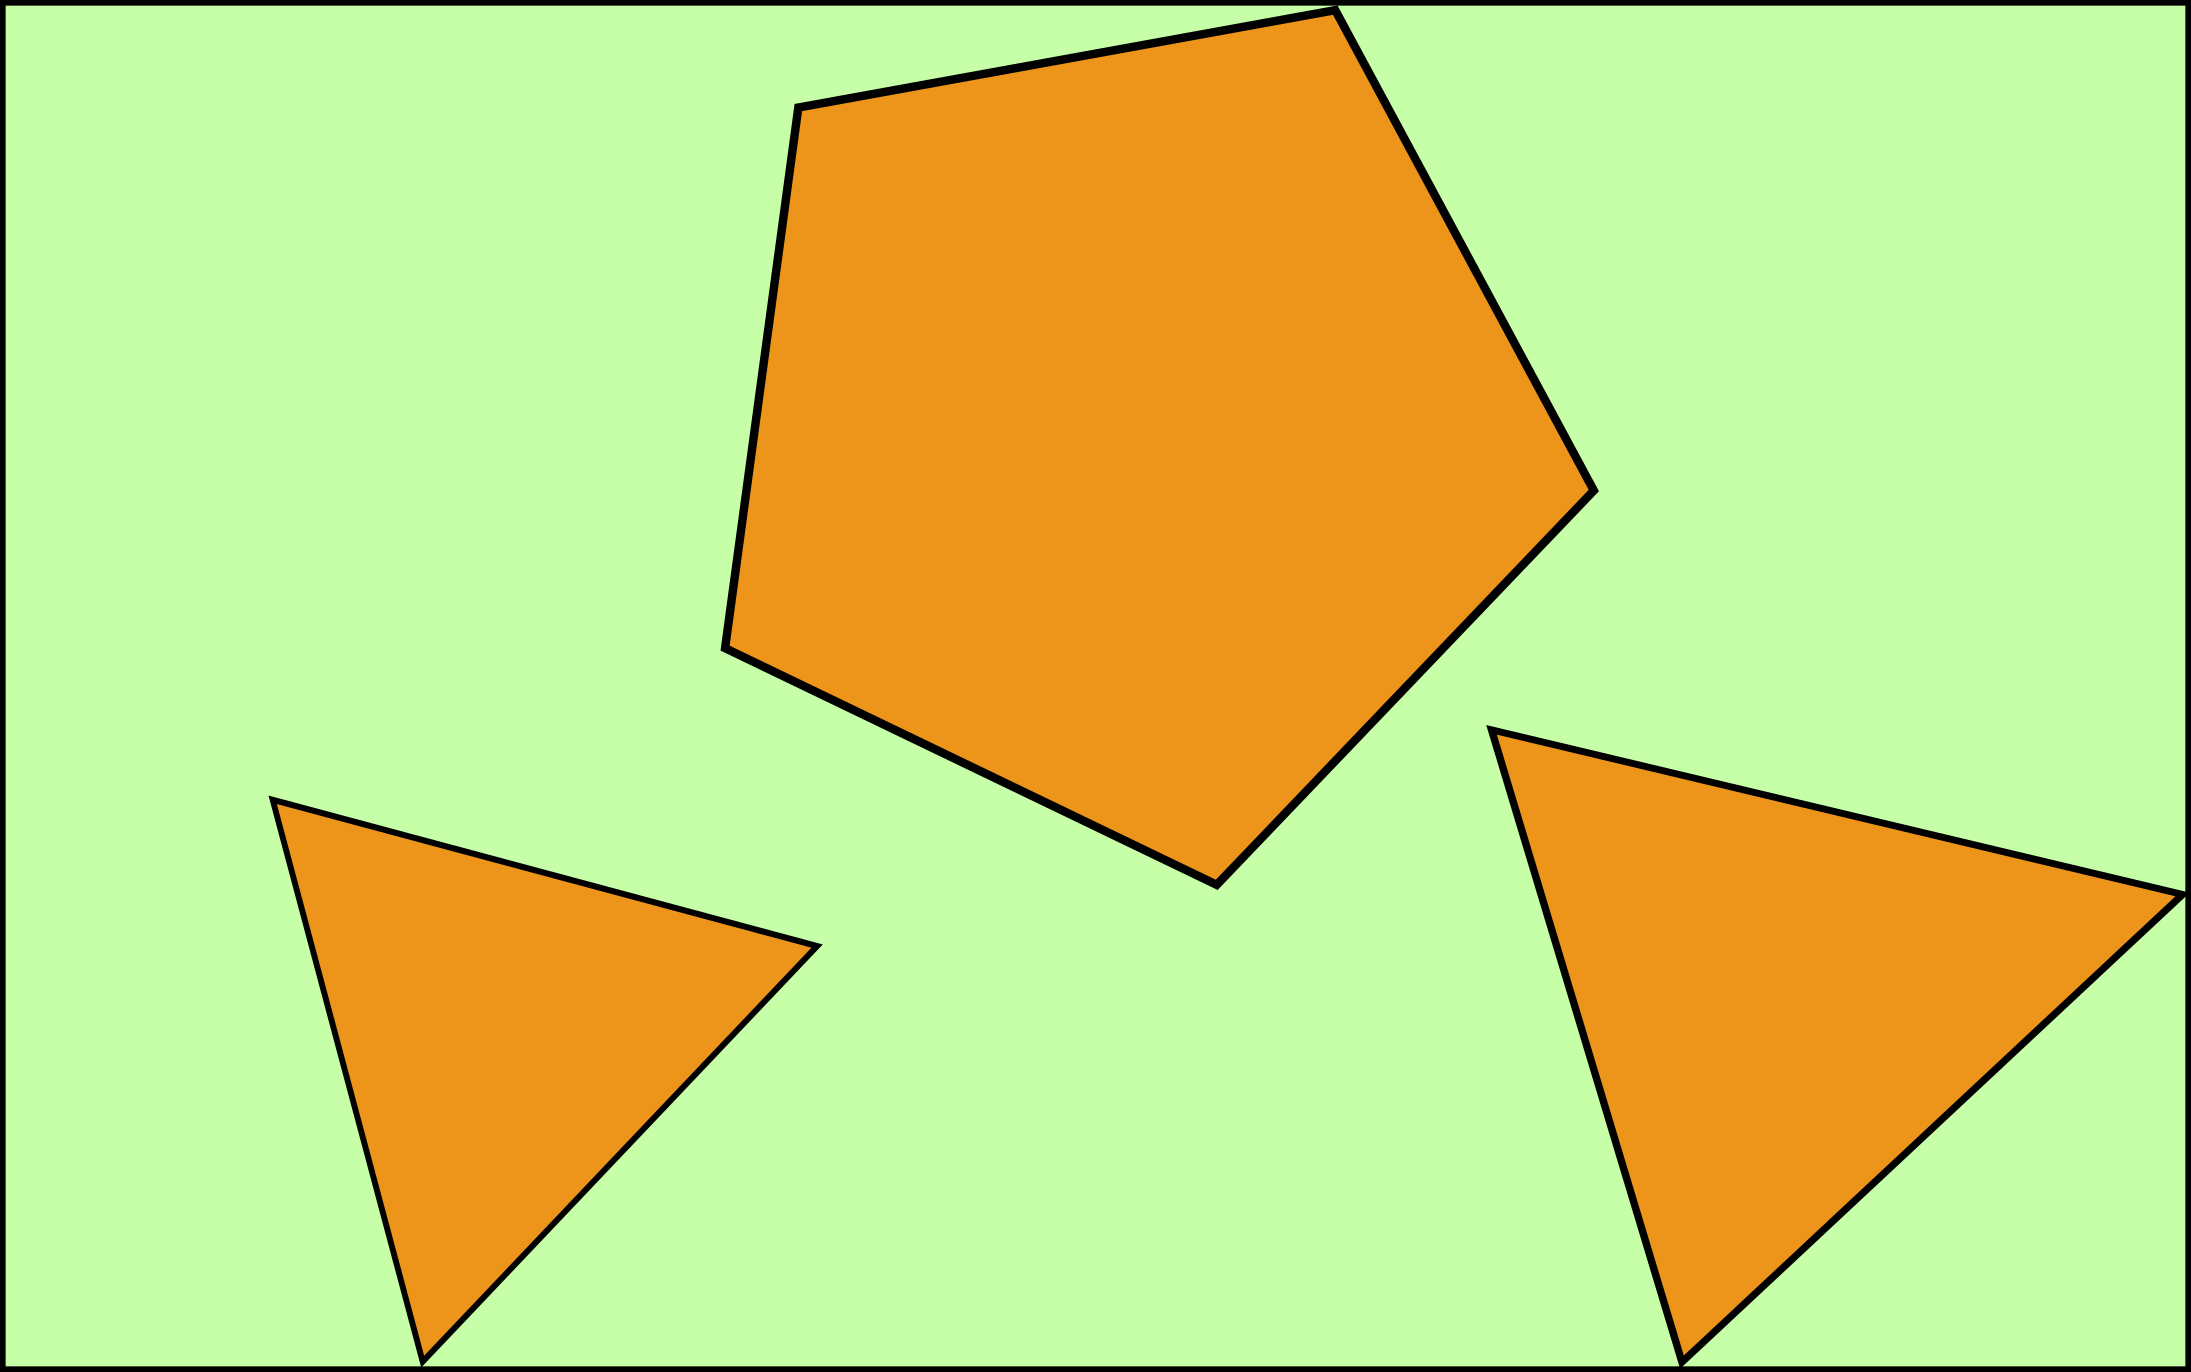
\includegraphics[width=0.70000\textwidth]{img/cellDec_es.png}\\[2\baselineskip]

\begin{enumerate}
\def\labelenumi{\alph{enumi}.}
\item
  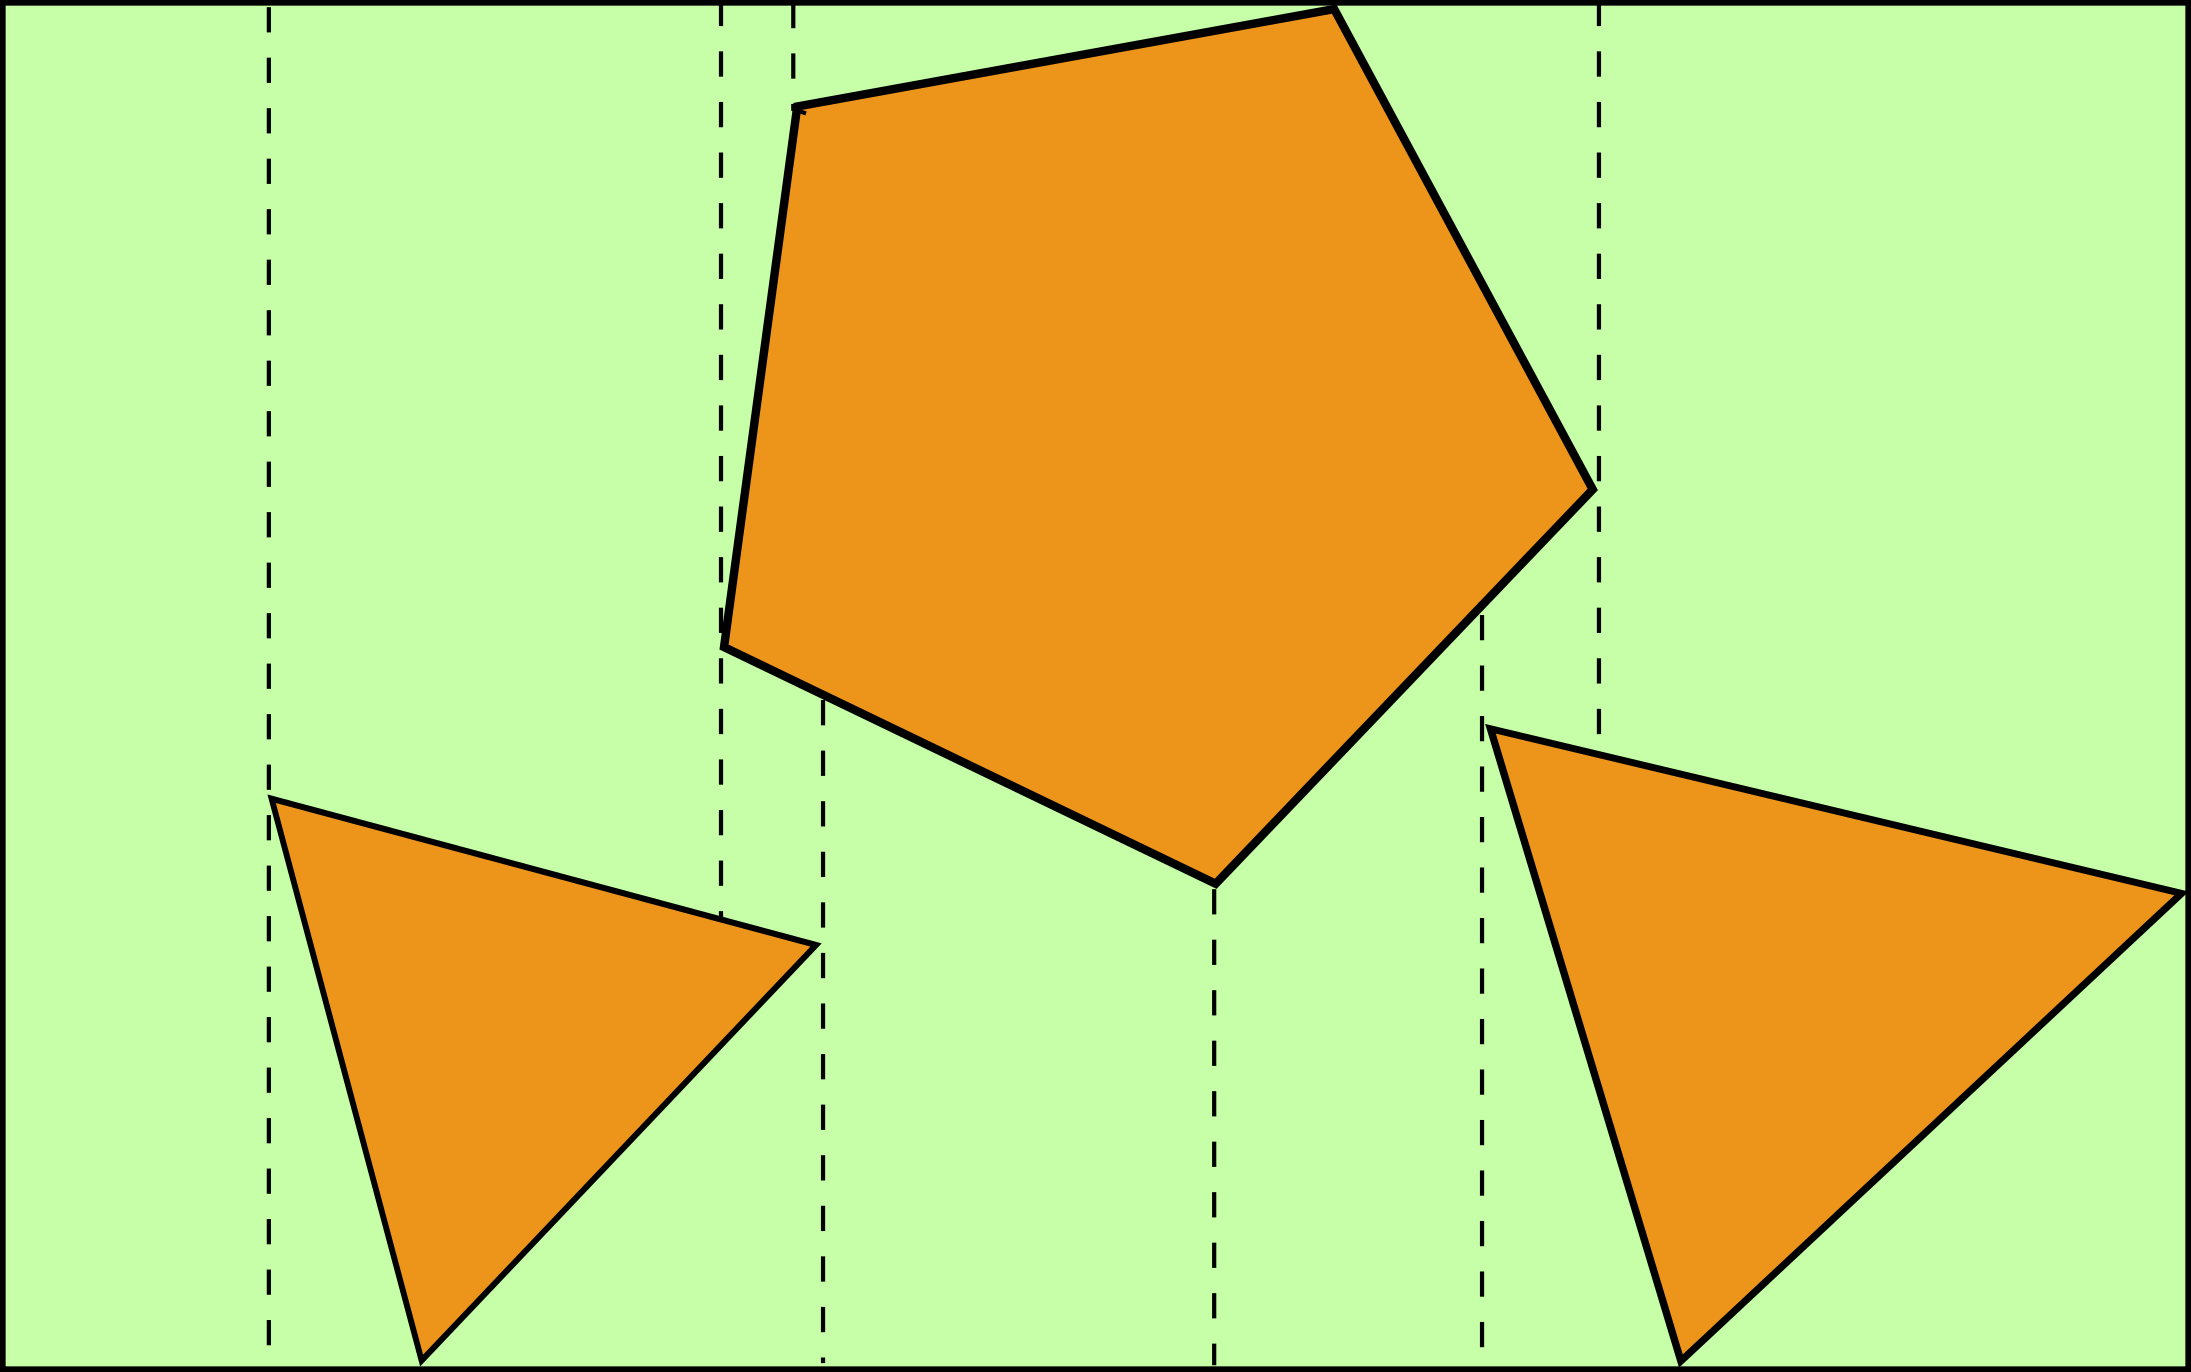
\includegraphics[width=0.50000\textwidth]{img/cellDec_es_sol1.png}
\item
  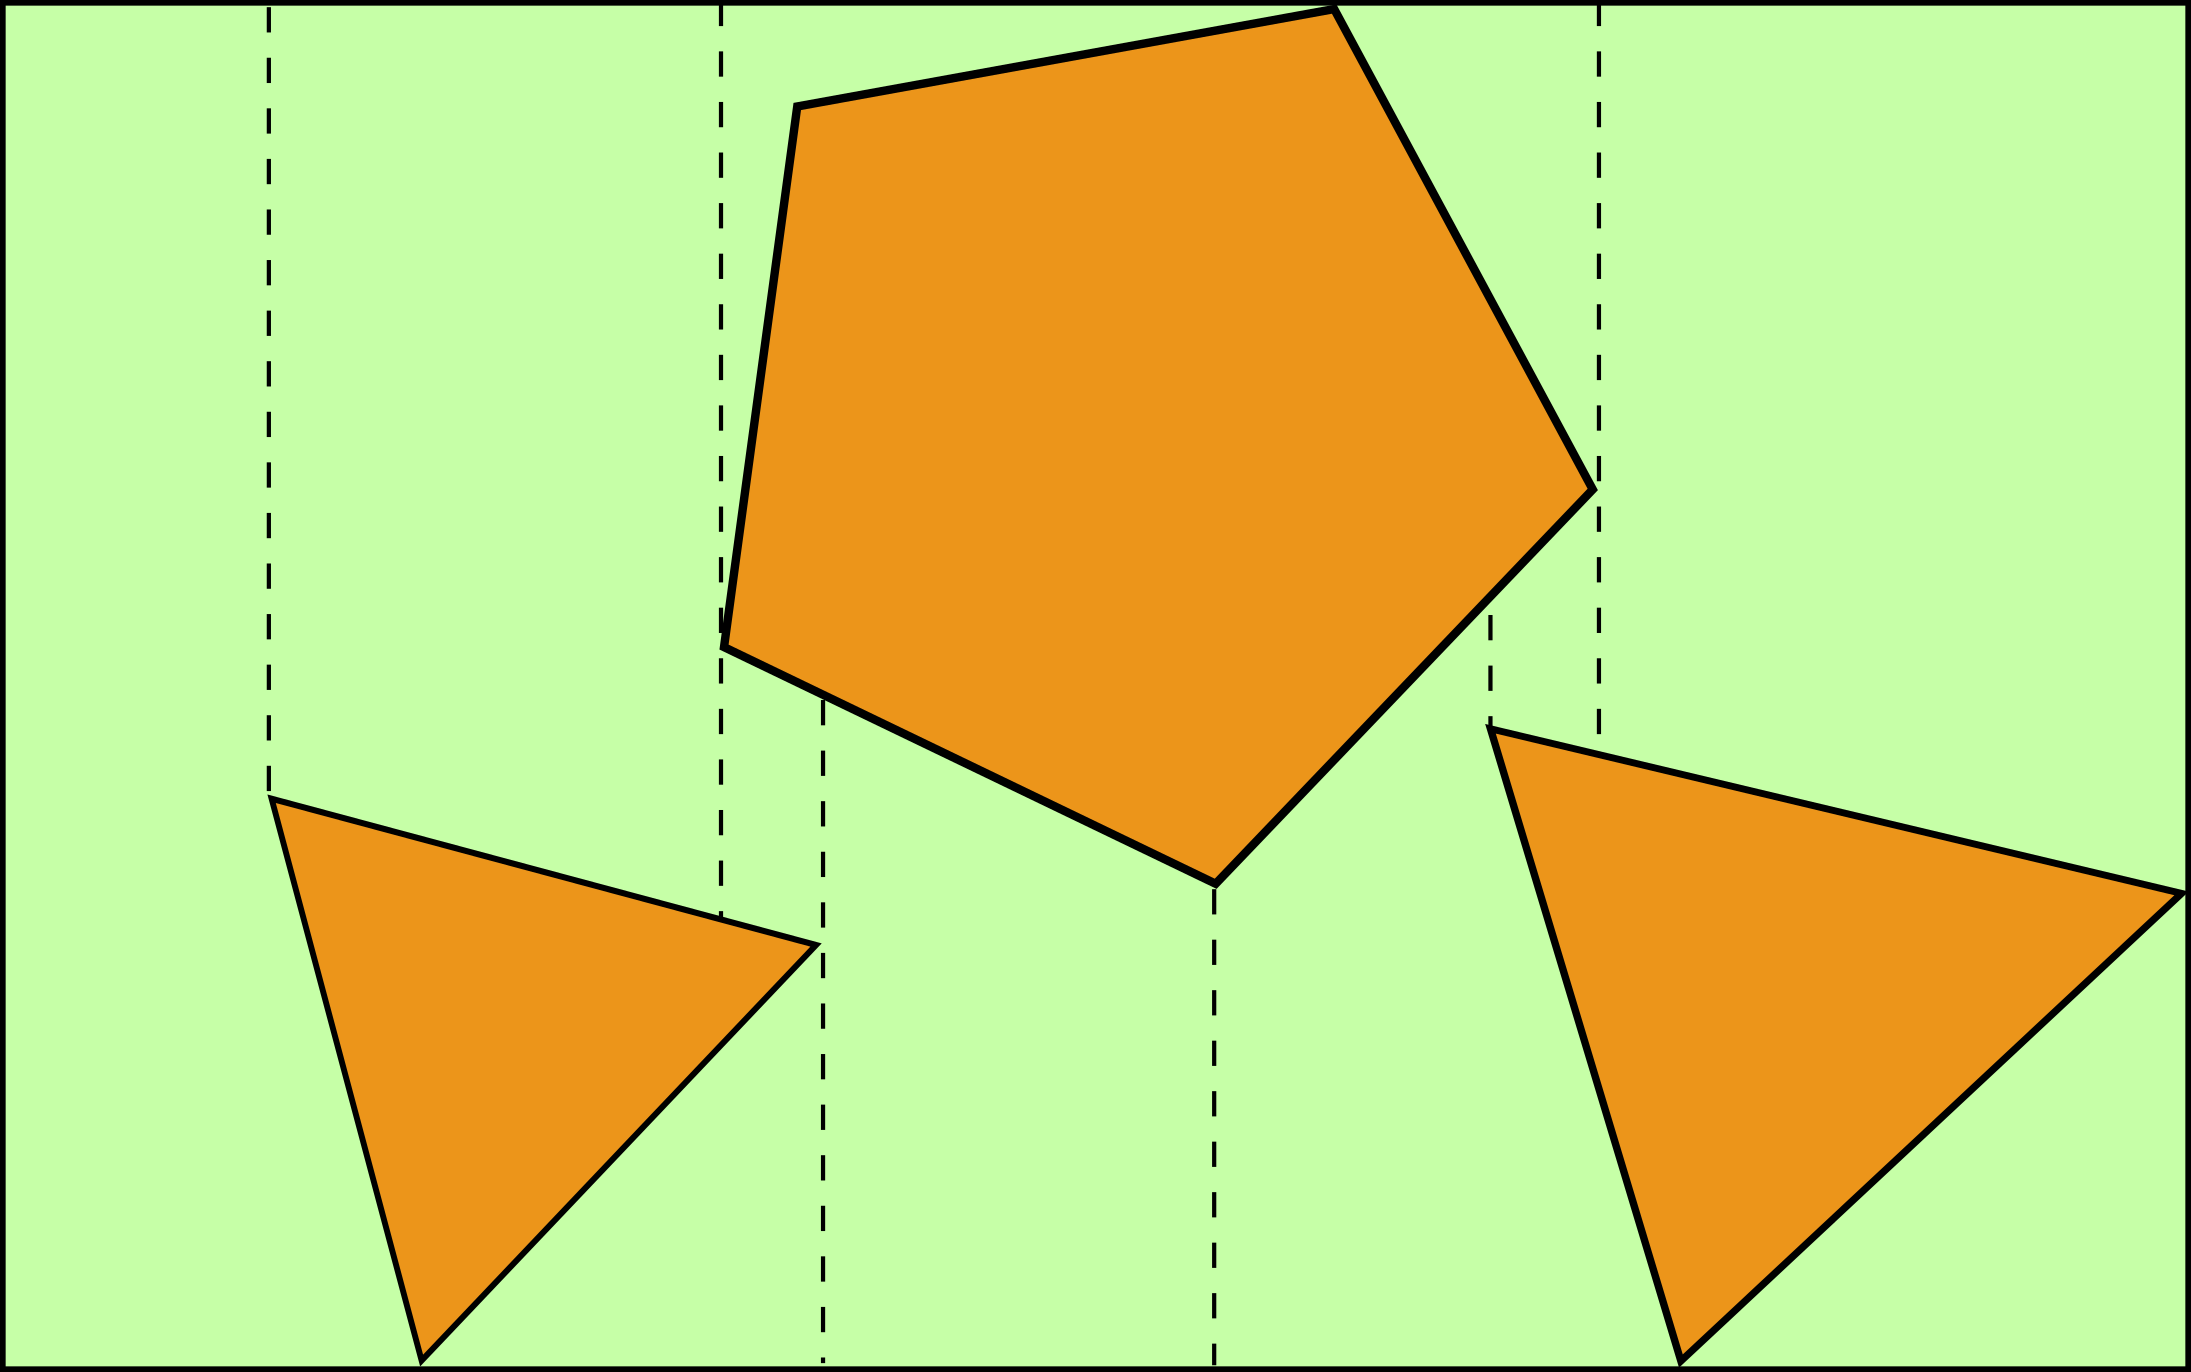
\includegraphics[width=0.50000\textwidth]{img/cellDec_es_sol2.png}
\item
  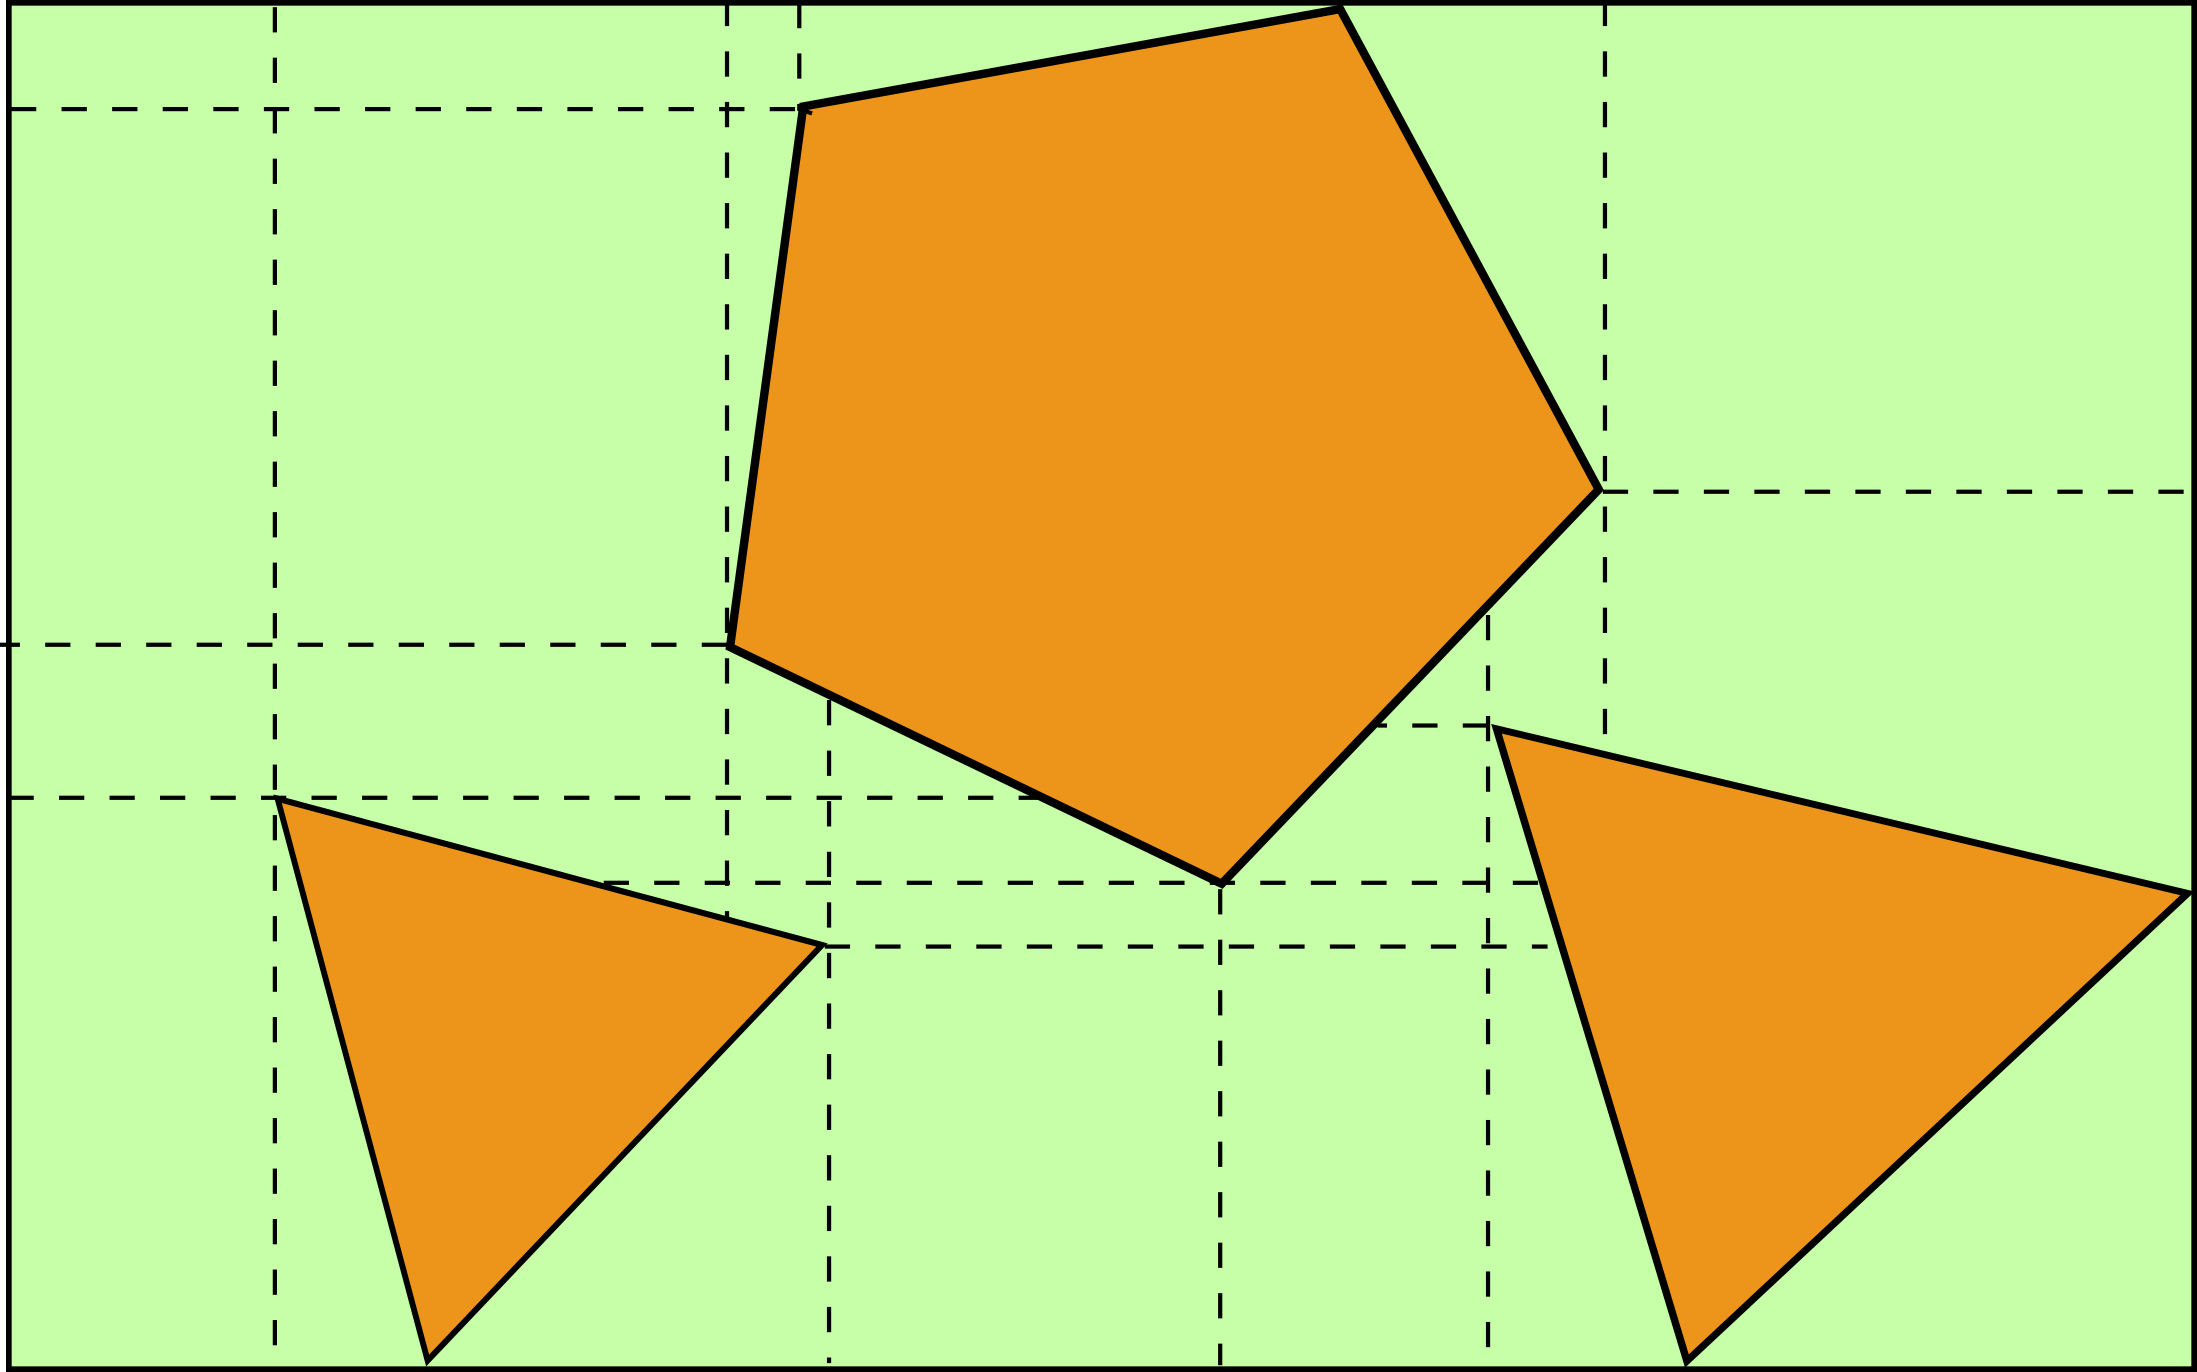
\includegraphics[width=0.50000\textwidth]{img/cellDec_es_sol3.png}
\end{enumerate}

\item Come sono collegati i vertici del grafo ottenuto dalla decomposizione cellulare del campo di lavoro della domanda precedente?

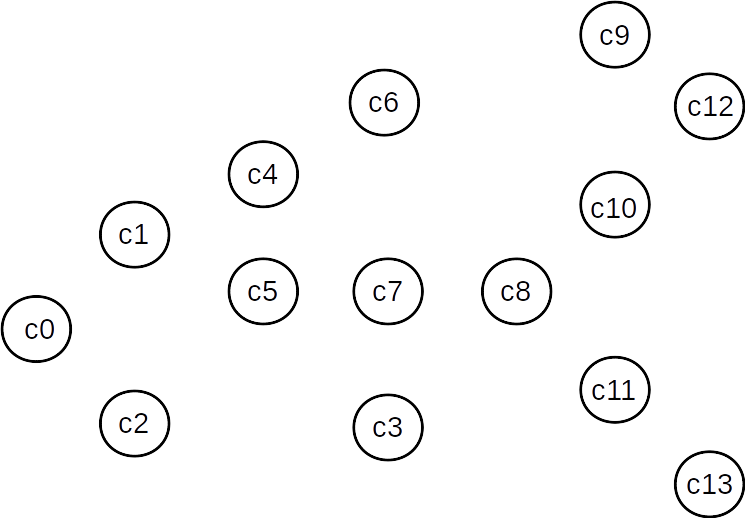
\includegraphics[width=0.70000\textwidth]{img/cellDec_grafo_es.png}\\[2\baselineskip]

\begin{enumerate}
\def\labelenumi{\alph{enumi}.}
\item
  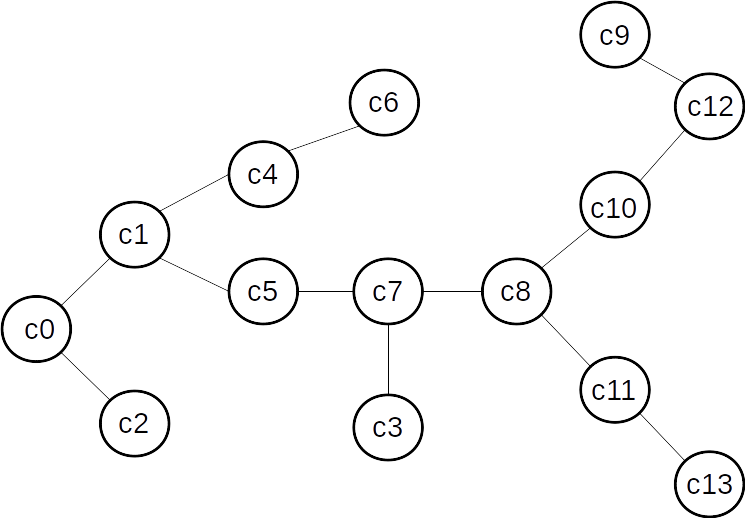
\includegraphics[width=0.50000\textwidth]{img/cellDec_grafo_es_sol1.png}
\item
  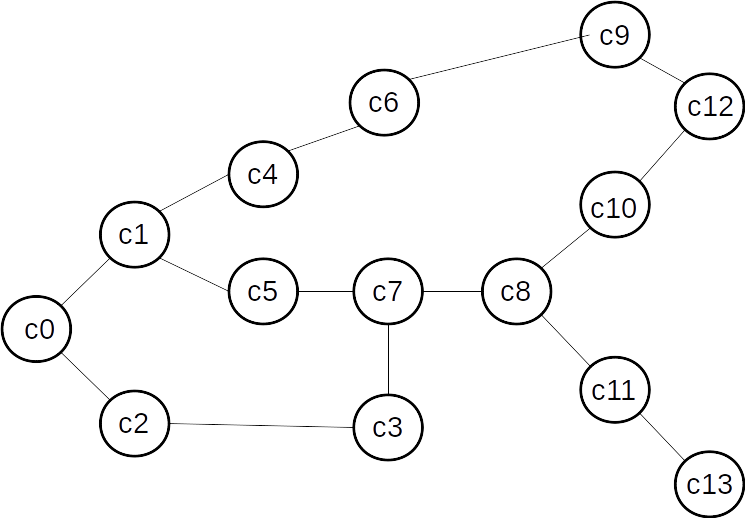
\includegraphics[width=0.50000\textwidth]{img/cellDec_grafo_es_sol2.png}
\item
  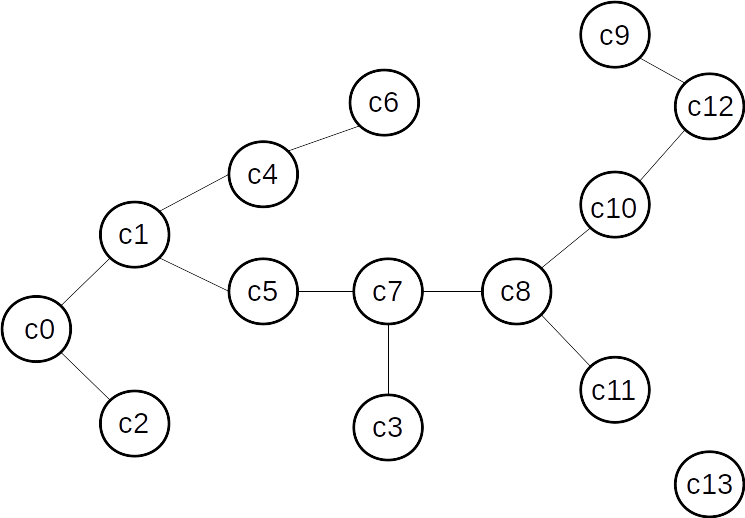
\includegraphics[width=0.50000\textwidth]{img/cellDec_grafo_es_sol3.png}
\end{enumerate}

\end{enumerate}
\newpage


\section{Creazione di un grafo}

\begin{wrapfigure}{L}{0.5\textwidth}
  \centering
  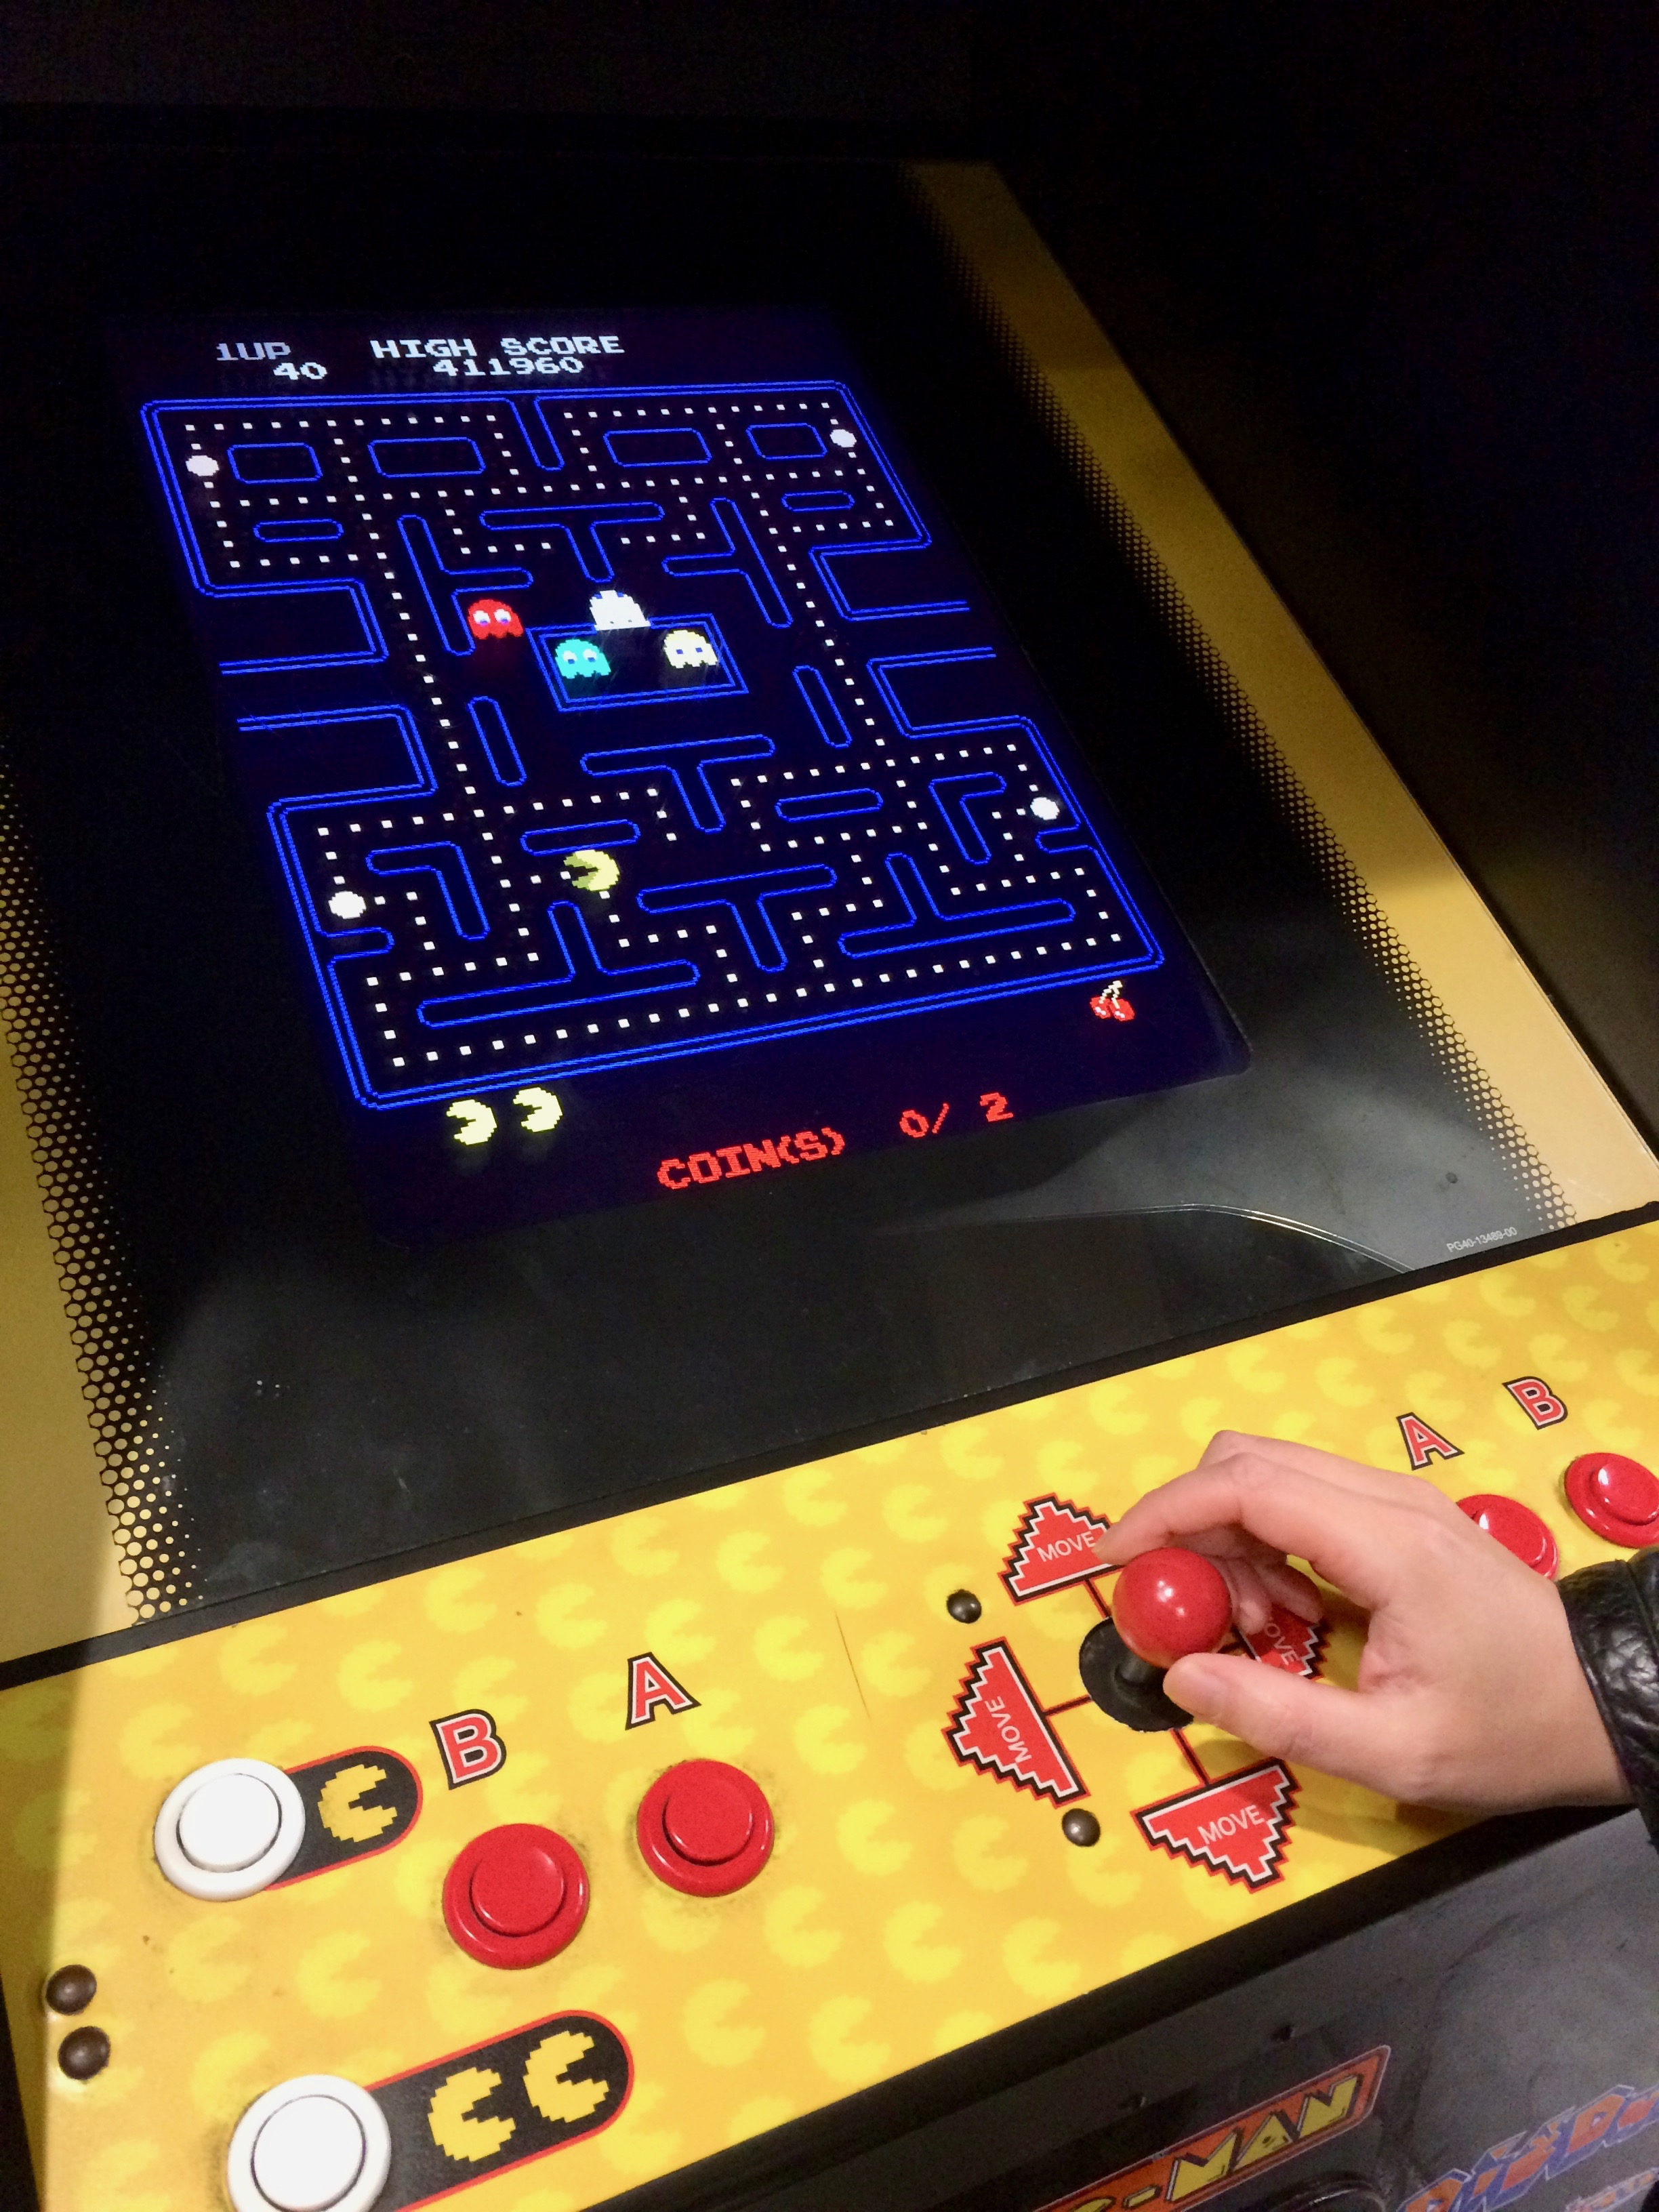
\includegraphics[width=0.5\textwidth]{img/imgConLicenza/postazione/postazione.jpg}
  \caption{Postazione Arcade di Pac-Man.}
  \label{postazione}
\end{wrapfigure}

Nell'informatica, i grafi sono implementati come strutture dati e funzioni che agiscono su queste.\\
Esistono diversi modelli di grafi che sono adatti a diversi scenari. Si può scegliere il modello giusto per uno scenario d'uso specifico al fine di semplificare l'implementazione o il riutilizzo del codice.\\
Nell'algoritmo boustrophedon il grafo è stato implementato da una matrice di strutture ognuna delle quali rappresenta un vertice del grafo. Ora, sebbene il labirinto rimane lo stesso, si propone un'implementazione diversa, basata più sugli archi che non sui vertici. Vediamo come.

\subsection{Grafo con numero variabile di archi}
Affrontiamo il problema della costruzione di un grafo che abbia un numero variabile di archi per ciascun vertice. Il labirinto di Pac-Man infatti può anche essere pensato come un labirinto di corridoi che si intersecano. Usando questo modello, un grafo più rappresentativo è quello in cui le intersezioni tra i corridoi (incroci) sono i vertici del grafo e i corridoi stessi sono gli archi.

Si confronti questo modello con quello usato nell'esempio del boustrophedon dove abbiamo usato un grafo che rappresentasse tutte le celle della tabella (matrice) del labirinto, ognuna collegata alle sue quattro celle vicine.


Per creare un tale grafo possiamo analizzare il labirinto partendo da un incrocio (intersezione) che rappresenterà il primo vertice, e aggiungere ad esso degli archi per ogni corridoio presente nell'incrocio. Quindi, seguiamo il corridoio aggiunto fino al prossimo incrocio, e questo sarà il secondo vertice del grafo. Ripetendo questa procedura per ogni corridoio, copriremo l'intero labirinto ottenendo il grafo del labirinto di Pac-Man.\\
Come esseri umani non abbiamo bisogno di un algoritmo formale per farlo, siamo semplicemente in grado di farlo. In realtà, il compito diventerebbe difficile se avessimo un labirinto molto grande e in una situazione del genere avremo bisogno di un algoritmo da seguire per non perderci.\\
In questa sezione insegniamo all'agent Pac-Man come creare un grafo ``Vertici e archi'' durante il gioco. Poiché il grafo non è noto all'agent all'inizio del gioco (ha bisogno di percorrere il labirinto per crearlo), stiamo ancora studiando lo scenario PO.

\subsection{L'agent}

L'obiettivo è fare in modo che l'agent generi un grafo del labirinto usando osservazioni online (tempo reale).\\
In ogni ciclo di gioco Pac-Man può solo osservare le celle adiacenti alla sua posizione corrente verificando se appartengono a corridoi accessibili o a pareti del labirinto. Ogni cella del labirinto ha otto celle vicine. Per generare il grafo, Pac-Man dovrebbe considerare ciascuna di esse, comunque sappiamo che l'architettura a labirinto non consente movimenti obliqui, quindi possiamo limitare l'agent Pac-Man a controllare solo le celle vicine nelle direzioni su, destra, giù e sinistra.\\
Pac-Man classifica come appartenente a un arco ogni cella che ha solo due vicini accessibili e come vertice quelle che ne hanno tre o più.

\subsubsection{Strutture dati}

Dalla teoria sappiamo che \emph{un grafo può essere rappresentato come un insieme di vertici e un insieme di archi i quali collegano ciascuno una coppia di vertici (non più di due).}

Come mostrato nel codice seguente, un arco è rappresentato attraverso la struttura (\texttt{agri\_Colligatio}) ed ha due vertici (\texttt{agri\_Vertex}) come la sua definizione formale dalla teoria dei grafi.

\begin{spacing}{0.9}
  \begin{small}
    \begin{tcolorbox}
\begin{verbatim}
typedef struct colligatio {
  agri_Vertex ab, ad;
  versus discessus, meta;
  int longitudo;
} agri_Colligatio; 
\end{verbatim}
    \end{tcolorbox}
  \end{small}
\end{spacing}

La teoria dei grafi non specifica cosa sia un vertice perché ciò dipende da quello che si vuol rappresentare con esso. Ad esempio, un vertice potrebbe essere una persona, come abbiamo visto nel famoso esempio del Zachary's karate club, oppure potrebbe essere uno scaffale di un magazzino, ma anche solo un indice numerico astratto.\\
Di seguito, rappresentiamo i vertici come tipi \texttt{struct} per poter aggiungere loro attributi di riga e colonna oltre al loro indice che li identifica nel labirinto.

\begin{spacing}{0.9}
  \begin{small}
    \begin{tcolorbox}
\begin{verbatim}
typedef struct {
  int linea;
  int columna;
  int index;
  int ianua[PORTE];
} agri_Vertex; 
\end{verbatim}
    \end{tcolorbox}
  \end{small}
\end{spacing}

Non è necessario creare un file con queste \texttt{struct} perché sono già presenti nei file di libreria libagri .

Nel codice in appendice \texttt{gioca\_tuki\_generagrafo.c}, Pac-Man costruisce il grafo mentre vaga per il labirinto. Ad ogni ciclo di gioco classifica la sua cella come un vertice o parte di un arco. La decisione viene presa contando il numero di celle vicine accessibili. Se ce ne sono due, Pac-Man si trova su un arco del grafo, altrimenti se ce ne sono più di due, Pac-Man si trova su un vertice come mostra il codice \emph{semplificato} di seguito.

\begin{spacing}{0.9}
  \begin{small}
    \begin{tcolorbox}
\begin{verbatim}
int nd = 0;
for(int k=0; k<4; k++)
  nd += (1*oggetto_accessibile(vicino[k]));

/* 
   È vero se nel ciclo di gioco corrente 
   viene rilevato un nodo 
*/
bool nodo_rilevato = false;
if(nd>2)
  {
    /* 
       Se siamo qui, Tuki è su un vertice 
    */
    int vertice_a = agri_Verticem_quaero(g,i,j);
    if(vertice_a<0)
      {
        vertice_a = vertici_contati;
        vertici_contati++;
      }    
  }
\end{verbatim}
    \end{tcolorbox}
  \end{small}
\end{spacing}

\textsc{Take home message:} in C, un grafo può essere implementato con una lista collegata i cui elementi sono gli archi.

\subsubsection{Compilazione ed esecuzione}

Si compili il codice con le opzioni specificate nel seguito:\\

\texttt{\textasciitilde{}/grafi\textbackslash{}\$ ./compila.sh PacMan/gioca\_tuki\_generagrafo.c\\ 0 50}\\

Si lanci specificando nessun fantasma:\\

\texttt{\textasciitilde{}/grafi\textbackslash{}\$ ./tuki5.game 0}\\

Ciò che si vedrà nel terminale potrebbe sorprendere perché nulla è cambiato dall'esecuzione del codice sviluppato per l'agent random.\\
Però questa è solo metà della storia, bisogna continuare a leggere per scoprire l'altra metà.

\subsection{Produzione del grafo}\label{tocux5f41}

Nel labirinto di Pac-Man, ogni arco è un corridoio che collega direttamente due incroci. Poiché ci sono 34 intersezioni nel labirinto, il grafo risultante avrà 34 vertici.

Questo è diverso dalla rappresentazione del boustrophedon, in cui ogni cella del labirinto è un vertice collegato da archi \emph{virtuali} alle sue quattro celle vicine, il tutto risultante in un numero maggiore di vertici nel grafo.

Per avere una rappresentazione grafica del grafo, vediamo che un grafo può essere rappresentato come una matrice quadrata i cui indici di colonna e riga sono i vertici. Costruiamo la matrice in modo che ogni elemento valga 1 o 0.\\

Agli elementi della matrice può essere assegnato anche un valore non binario. Per esempio, se si sta rappresentando un grafo delle connessioni stradali tra le città, si potrebbe assegnare agli elementi della matrice la distanza tra le due città individuate dalla riga e dalla colonna della matrice stessa.\\

L'elemento nella riga $i$ e colonna $j$ è diverso da 0 se esiste un bordo che collega i vertici $i$ e $j$ (vedi fig. \ref{grafoProdotto})

\begin{figure}
  \begin{subfigure}[b]{0.49\textwidth}
    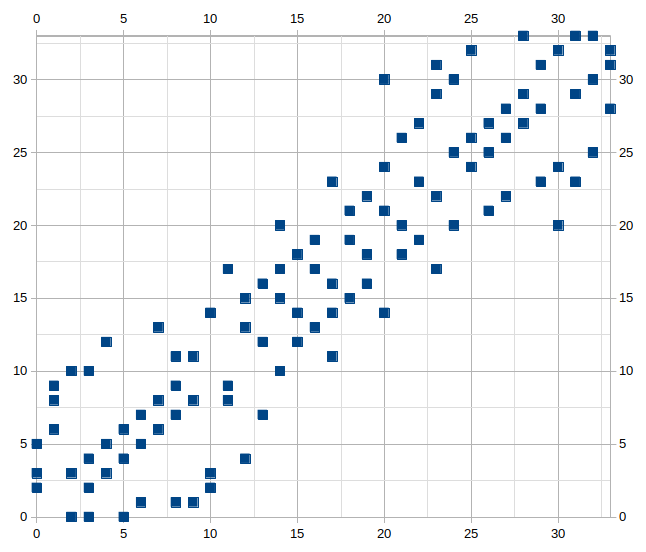
\includegraphics[width=\textwidth]{img/pacman_grafo.png}
    \label{grafoProdotto_1}
   \end{subfigure}
  \begin{subfigure}[b]{0.49\textwidth}
    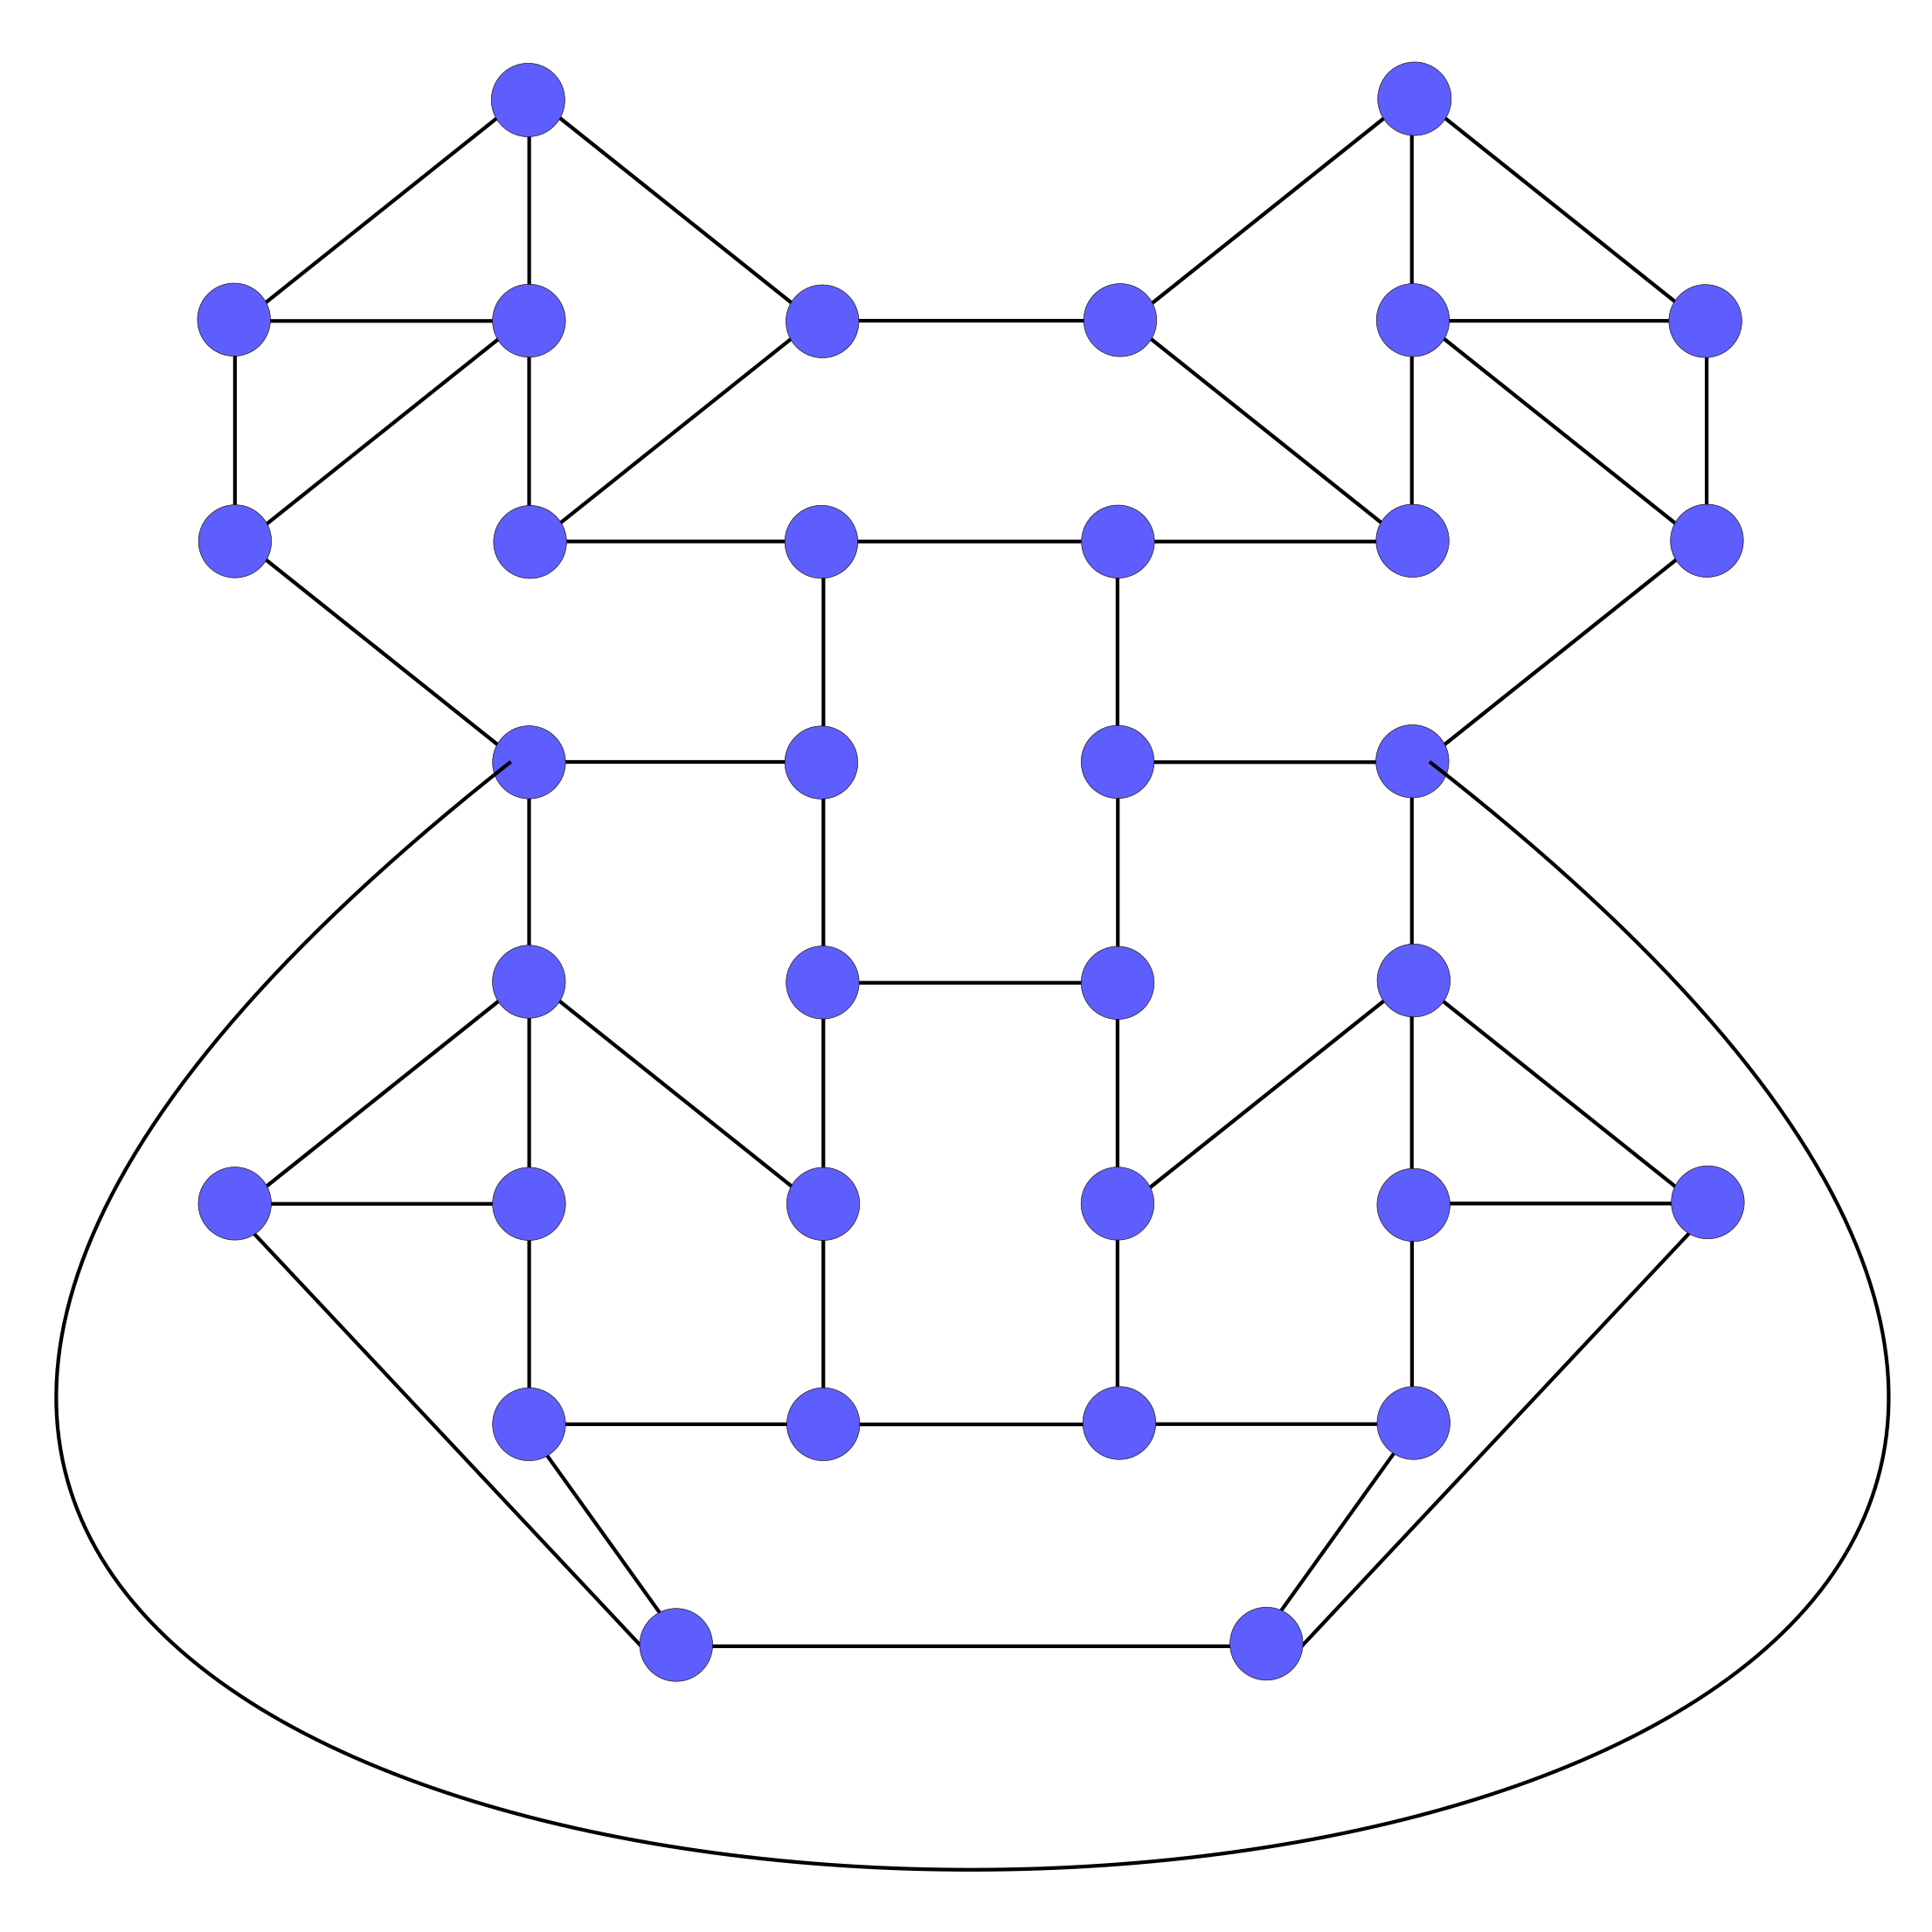
\includegraphics[width=\textwidth]{img/tuki5_grafo.png}
    \label{grafoProdotto_2}
  \end{subfigure}
  \caption{Rappresentazione matriciale del grafo del labirinto di Pac-Man (sinistra). I vertici sono ordinati da in alto a sinistra a in basso a destra. Rappresentazione vertici-archi per lo stesso grafo (destra)}
  \label{grafoProdotto}
\end{figure}

Pac-Man esplora il grafo scegliendo una direzione per ogni vertice che incontra. Diverse sequenze di gioco produrranno quindi decisioni di direzione diverse e quindi grafi diversi (vedi figura \ref{grafiProdotti}).\\
Comunque, se Pac-Man ha completato il labirinto, ci aspettiamo che ci sia una relazione specifica tra i grafi prodotti.\\
Diversamente, se Pac-Man viene mangiato da un fantasma prima di completare il gioco, ovviamente non esplorerà l'intero labirinto, il che significa che ogni corsa produrrà casualmente un grafo diverso.\\
Esistono quindi due diverse situazioni:

\begin{enumerate}
\def\labelenumi{\alph{enumi}.}
\item
  i grafi prodotti corrispondono all'intero labirinto
\item
  i grafi prodotti non corrispondono all'intero labirinto
\end{enumerate}

in entrambe le situazioni non si prevede che il grafo prodotto sia lo stesso

Ovviamente si può immaginare che, dato un labirinto, il suo grafo non possa dipendere fortemente dal percorso specificato scelto per esplorarlo. Infatti, se due grafi, nonostante il loro diverso aspetto, corrispondono allo stesso labirinto, si dice che sono isomorfi, cioè è possibile ottenere l'uno dall'altro con una semplice permutazione delle etichette dei loro vertici.\\
Questo è il caso di due grafi ottenuti da due esecuzioni di Pac-Man completate (tutti gli archi attraversati). D'altra parte, i grafi ottenuti dalle partite vinte dai fantasmi saranno generalmente incompleti (vedi fig. 10) e l'isomorfismo tra loro non è garantito. Tuttavia, questi grafi incompleti sono subisomorfi a quelli completi.

\begin{figure}
  \centering
  \begin{subfigure}[b]{0.49\textwidth}
    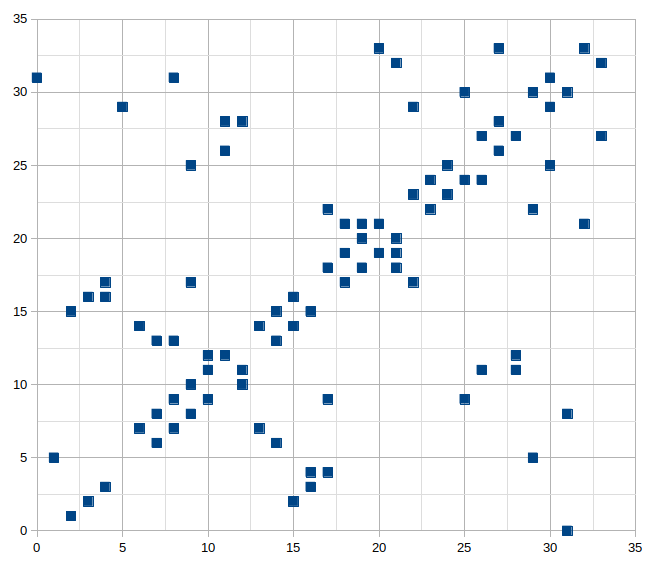
\includegraphics[width=\textwidth]{img/tuki_grafo_2.png}
   \end{subfigure}
  \begin{subfigure}[b]{0.49\textwidth}
    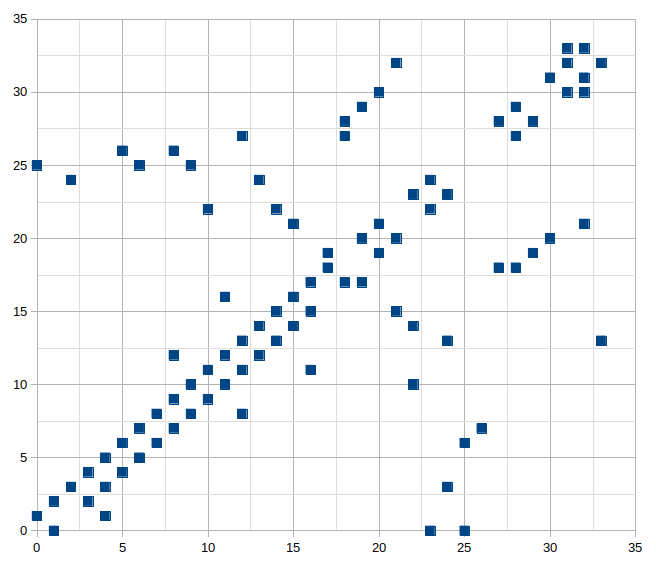
\includegraphics[width=\textwidth]{img/tuki_grafo.png}
  \end{subfigure}
  \caption{Rappresentazione matriciale del grafo del labirinto di Pac-Man. I vertici vengono ordinati non appena vengono scoperti dall'agent Pac-Man che vaga per il labirinto. Le immagini corrispondono a due diverse serie in cui Pac-Man ha completato l'intero labirinto}
  \label{grafiProdotti}
\end{figure}

\begin{figure}
  \centering
  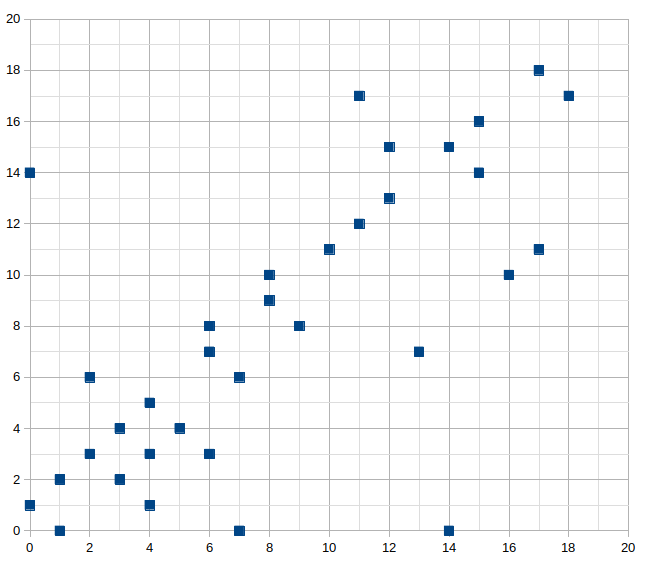
\includegraphics[width=0.5\textwidth]{img/tuki_grafo_parziale.png}
  \caption{Rappresentazione matriciale del grafo a labirinto Pac-Man. Pac-Man non ha completato l'esplorazione del grafico}
  \label{grafoParziale}
\end{figure}

\subsection{Stampa e analisi del grafo}

La rappresentazione \emph{visiva} del grafo è utile per analizzare più facilmente alcune proprietà del grafo come il grado (valenza) dei vertici. Questa rappresentazione può essere ottenuta tracciando su un piano cartesiano, i punti dati dalle coppie di indici dei vertici di ciascun arco.\\
Le figure \ref{grafoProdotto}, \ref{grafiProdotti} e \ref{grafoParziale} sono state ottenute tracciando un set di dati prodotto durante l'esecuzione del codice \\\texttt{gioca\_tuki\_generagrafo.c}. Per testarlo, si decommentino le istruzioni di stampa:

\begin{spacing}{0.9}
  \begin{small}
\begin{tcolorbox}
\begin{verbatim}
//stampa(g);
\end{verbatim}
    \end{tcolorbox}
  \end{small}
\end{spacing}


poi si compili il progetto nuovamente (come mostrato sopra) e lo si esegua. Questo genererà il file \texttt{grafi.csv} nella directory in esecuzione. Se si vuol essere sicuri di generare il grafo completo, si avvii il gioco senza fantasmi:\\

\texttt{
\textasciitilde{}/grafi\textbackslash{}\$ ./tuki5.game 0
}


Il file \texttt{grafi.csv} può essere usato per implementare facilmente il grafo in un programma basato sulla nota libreria C \emph{igraph} .

Supponiamo che il contenuto del file sia il seguente:

\begin{spacing}{0.9}
  \begin{small}
\begin{tcolorbox}
\begin{verbatim}
 23,32,
 22,31,
 16,19,
 ...
 2,3,
 1,2,
 0,1,
\end{verbatim}
    \end{tcolorbox}
  \end{small}
\end{spacing}

può essere usato per inizializzare l'array igraph\_real\_t edges1{[}{]} nel codice seguente:

\begin{spacing}{0.9}
  \begin{small}
\begin{tcolorbox}
\begin{verbatim}
#include <igraph.h>
#include <stdio.h>
//gcc -o cmp confronta.c-I/usr/local/include/igraph
//  -L/usr/local/lib -ligraph

int main(void) {
  igraph_t graph1,graph2;
  igraph_vector_t v1,v2;
  igraph_vector_t result;
  
  /* Tuki */
  igraph_real_t edges1[] =
    {
      23,32, 22,31, 16,19, 19,5,
      20,19, 7,13, 18,9, 33,28,
      33,30, 28,33, 20,16, 21,20,
      5,21, 0,7, 8,6, 10,8, 14,
      21, 13,12, 9,13, 24,18, 32,
      25, 33,26, 30,33, 28,30,
      29,28, 10,29, 11,10, 12,11,
      15,12, 16,15, 9,18, 13,
      9, 22,8, 31,22, 31,23, 32,
      31, 32,23, 31,32, 23,31,
      24,23, 25,24, 26,25, 27,26,
      28,27, 30,28, 29,30, 28,
      29, 27,28, 26,27, 25,26, 24,
      25, 23,24, 22,23, 8,22,
      21,14, 20,21, 19,20, 5,19, 2,
      1, 6,2, 15,14, 12,15,
      17,11, 18,17, 17,18, 11,17, 16,
      10, 15,16, 14,15, 1,
      0, 14,0, 0,14, 7,0, 13,7, 12,
      13, 11,12, 10,11, 8,10,
      9,8, 8,9, 6,8, 7,6, 6,7, 4,1,
      6,3, 2,6, 3,2, 4,3, 5,
      4, 4,5, 3,4, 2,3, 1,2, 0,1
    };

\end{verbatim}
    \end{tcolorbox}
  \end{small}
\end{spacing}

\begin{spacing}{0.9}
  \begin{small}
\begin{tcolorbox}
\begin{verbatim}
  
  /* PAC-MAN GRAPH */
  igraph_real_t edges2[] =
    {
      0,2,0,3,0,5,1,6,1,8,1,9,2,0,
      2,3,2,10,3,0,3,2,3,4,
      3,10,4,3,4,5,4,12,5,0,5,4,5,6,
      6,1,6,5,6,7,7,6,7,8,7,13,8,1,
      8,7,8,9,8,11,9,1,9,8,9,11,10,2,
      10,3,10,14,11,8,11,9,11,17,
      12,4,12,13,12,15,13,7,13,12,13,
      16,14,10,14,15,14,17,14,20,
      15,14,15,12,15,18,16,13,16,17,
      16,19,17,11,17,14,17,16,17,
      23,18,15,18,19,18,21,19,16,19,
      18,19,22,20,14,20,21,20,24,
      20,30,21,18,21,20,21,26,22,19,
      22,23,22,27,23,17,23,22,23,
      29,23,31,24,20,24,25,24,30,25,
      24,25,26,25,32,26,21,26,25,
      26,27,27,22,27,26,27,28,28,27,
      28,29,28,33,29,23,29,28,29,
      31,30,20,30,24,30,32,31,23,31,
      29,31,33,32,30,32,25,32,33,
      33,28,33,31,33,32
    };
  
  igraph_vector_view(&v1, edges1,
		     sizeof(edges1)/sizeof(double));
  igraph_create(&graph1, &v1, 0,
		IGRAPH_UNDIRECTED);
  
  igraph_vector_view(&v2, edges2,
		     sizeof(edges2)/sizeof(double));
  igraph_create(&graph2, &v2, 0,
		IGRAPH_UNDIRECTED);
  
  igraph_bool_t iso;
  igraph_subisomorphic(&graph2, &graph1,&iso);
  
  printf("%d\n",iso);
  igraph_destroy(&graph1);
  igraph_destroy(&graph2);
  
  return 0;
}
\end{verbatim}
    \end{tcolorbox}
  \end{small}
\end{spacing}

Si può immaginare che mentre il primo array rappresenta il grafo esplorato dall'agent, il secondo corrisponde a quello di figura \ref{grafoProdotto}.\\
La chiamata alla funzione \texttt{igraph\_subisomorphic} verifica se \texttt{graph1} sia isomorfo a un sotto-grafo di \texttt{graph2}.\\
La chiamata a \texttt{igraph\_isomorphic} (invece di \texttt{igraph\_subisomorphic}) potrebbe restituire $0$ poiché Pac-Man non avrebbe potuto attraversare alcuni degli archi dove non ci sono pillole, ovvero $12$-$13$, $13$-$16$ , $16$-$19$, $19$-$18$, $18$-$15$, $15$-$12$.

In questa sezione abbiamo mostrato il metodo per creare un grafo archi-vertici anche in condizioni PO. Nella prossima illustreremo come usare questo grafo per ottimizzare l'agent di Pac-Man.

\newpage
\section*{Box domande n.3}
\addcontentsline{toc}{section}{Box domande n.3}

\begin{enumerate}
\item Nell'algoritmo generagrafo, cosa differenzia una cella-vertice da una cella-arco?

\begin{enumerate}
\def\labelenumi{\alph{enumi}.}

\item
  Esistono solo celle-vertice, mentre gli archi sono collegamenti virtuali tra vertici
\item
  Una cella-vertice ha almeno 3 celle vicine accessibili, mentre una cella-arco ne ha solo 2
\item
  Niente, ad ogni esecuzione l'agent etichetta le celle come celle-vertice o celle-arco in maniera casuale
\end{enumerate}

\item Trova il grafo di questo labirinto utilizzando l'algoritmo generagrafo. Di quanti vertici e quanti archi è composto?

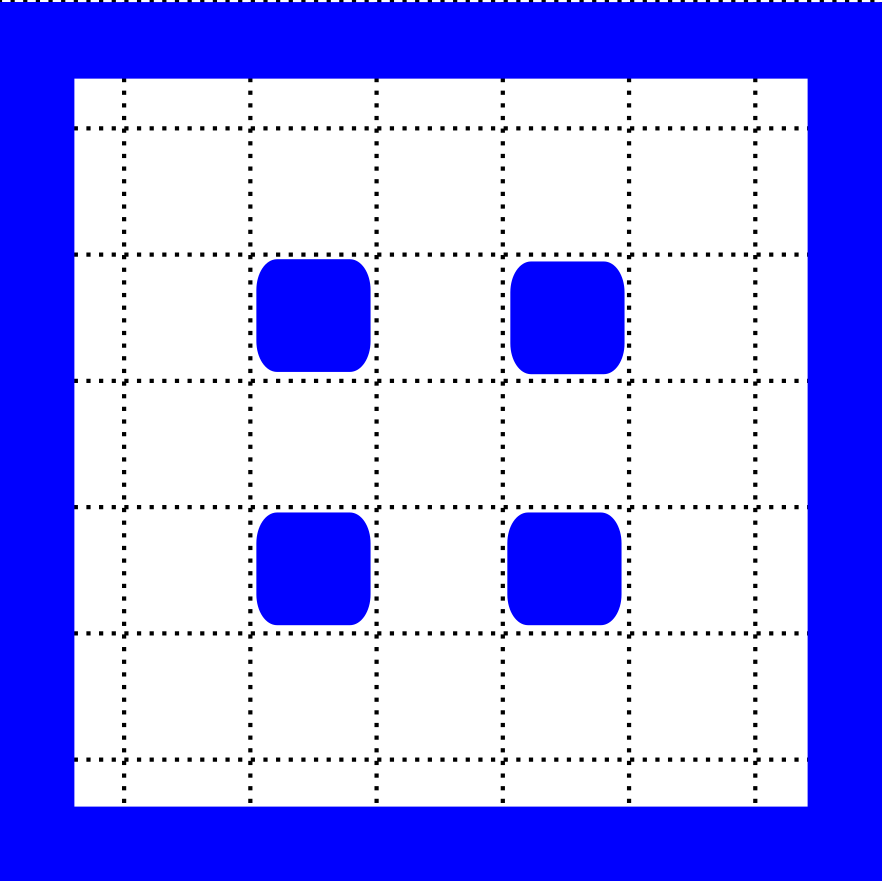
\includegraphics[width=0.50000\textwidth]{img/num_VerticiArchi_es.png}\\[2\baselineskip]

\begin{enumerate}
\def\labelenumi{\alph{enumi}.}

\item
  5 vertici, 8 archi
\item
  4 vertici, 4 archi
\item
  9 vertici, 12 archi
\end{enumerate}

\item Trova il grafo dello stesso labirinto utilizzando l'algoritmo boustrophedon. Di quanti vertici e quanti archi è composto?

\begin{enumerate}
\def\labelenumi{\alph{enumi}.}

\item
  9 vertici, 12 archi
\item
  25 vertici, 40 archi
\item
  21 vertici, 24 archi
\end{enumerate}

Dato il seguente grafo, qual è la sua matrice corrispondente?

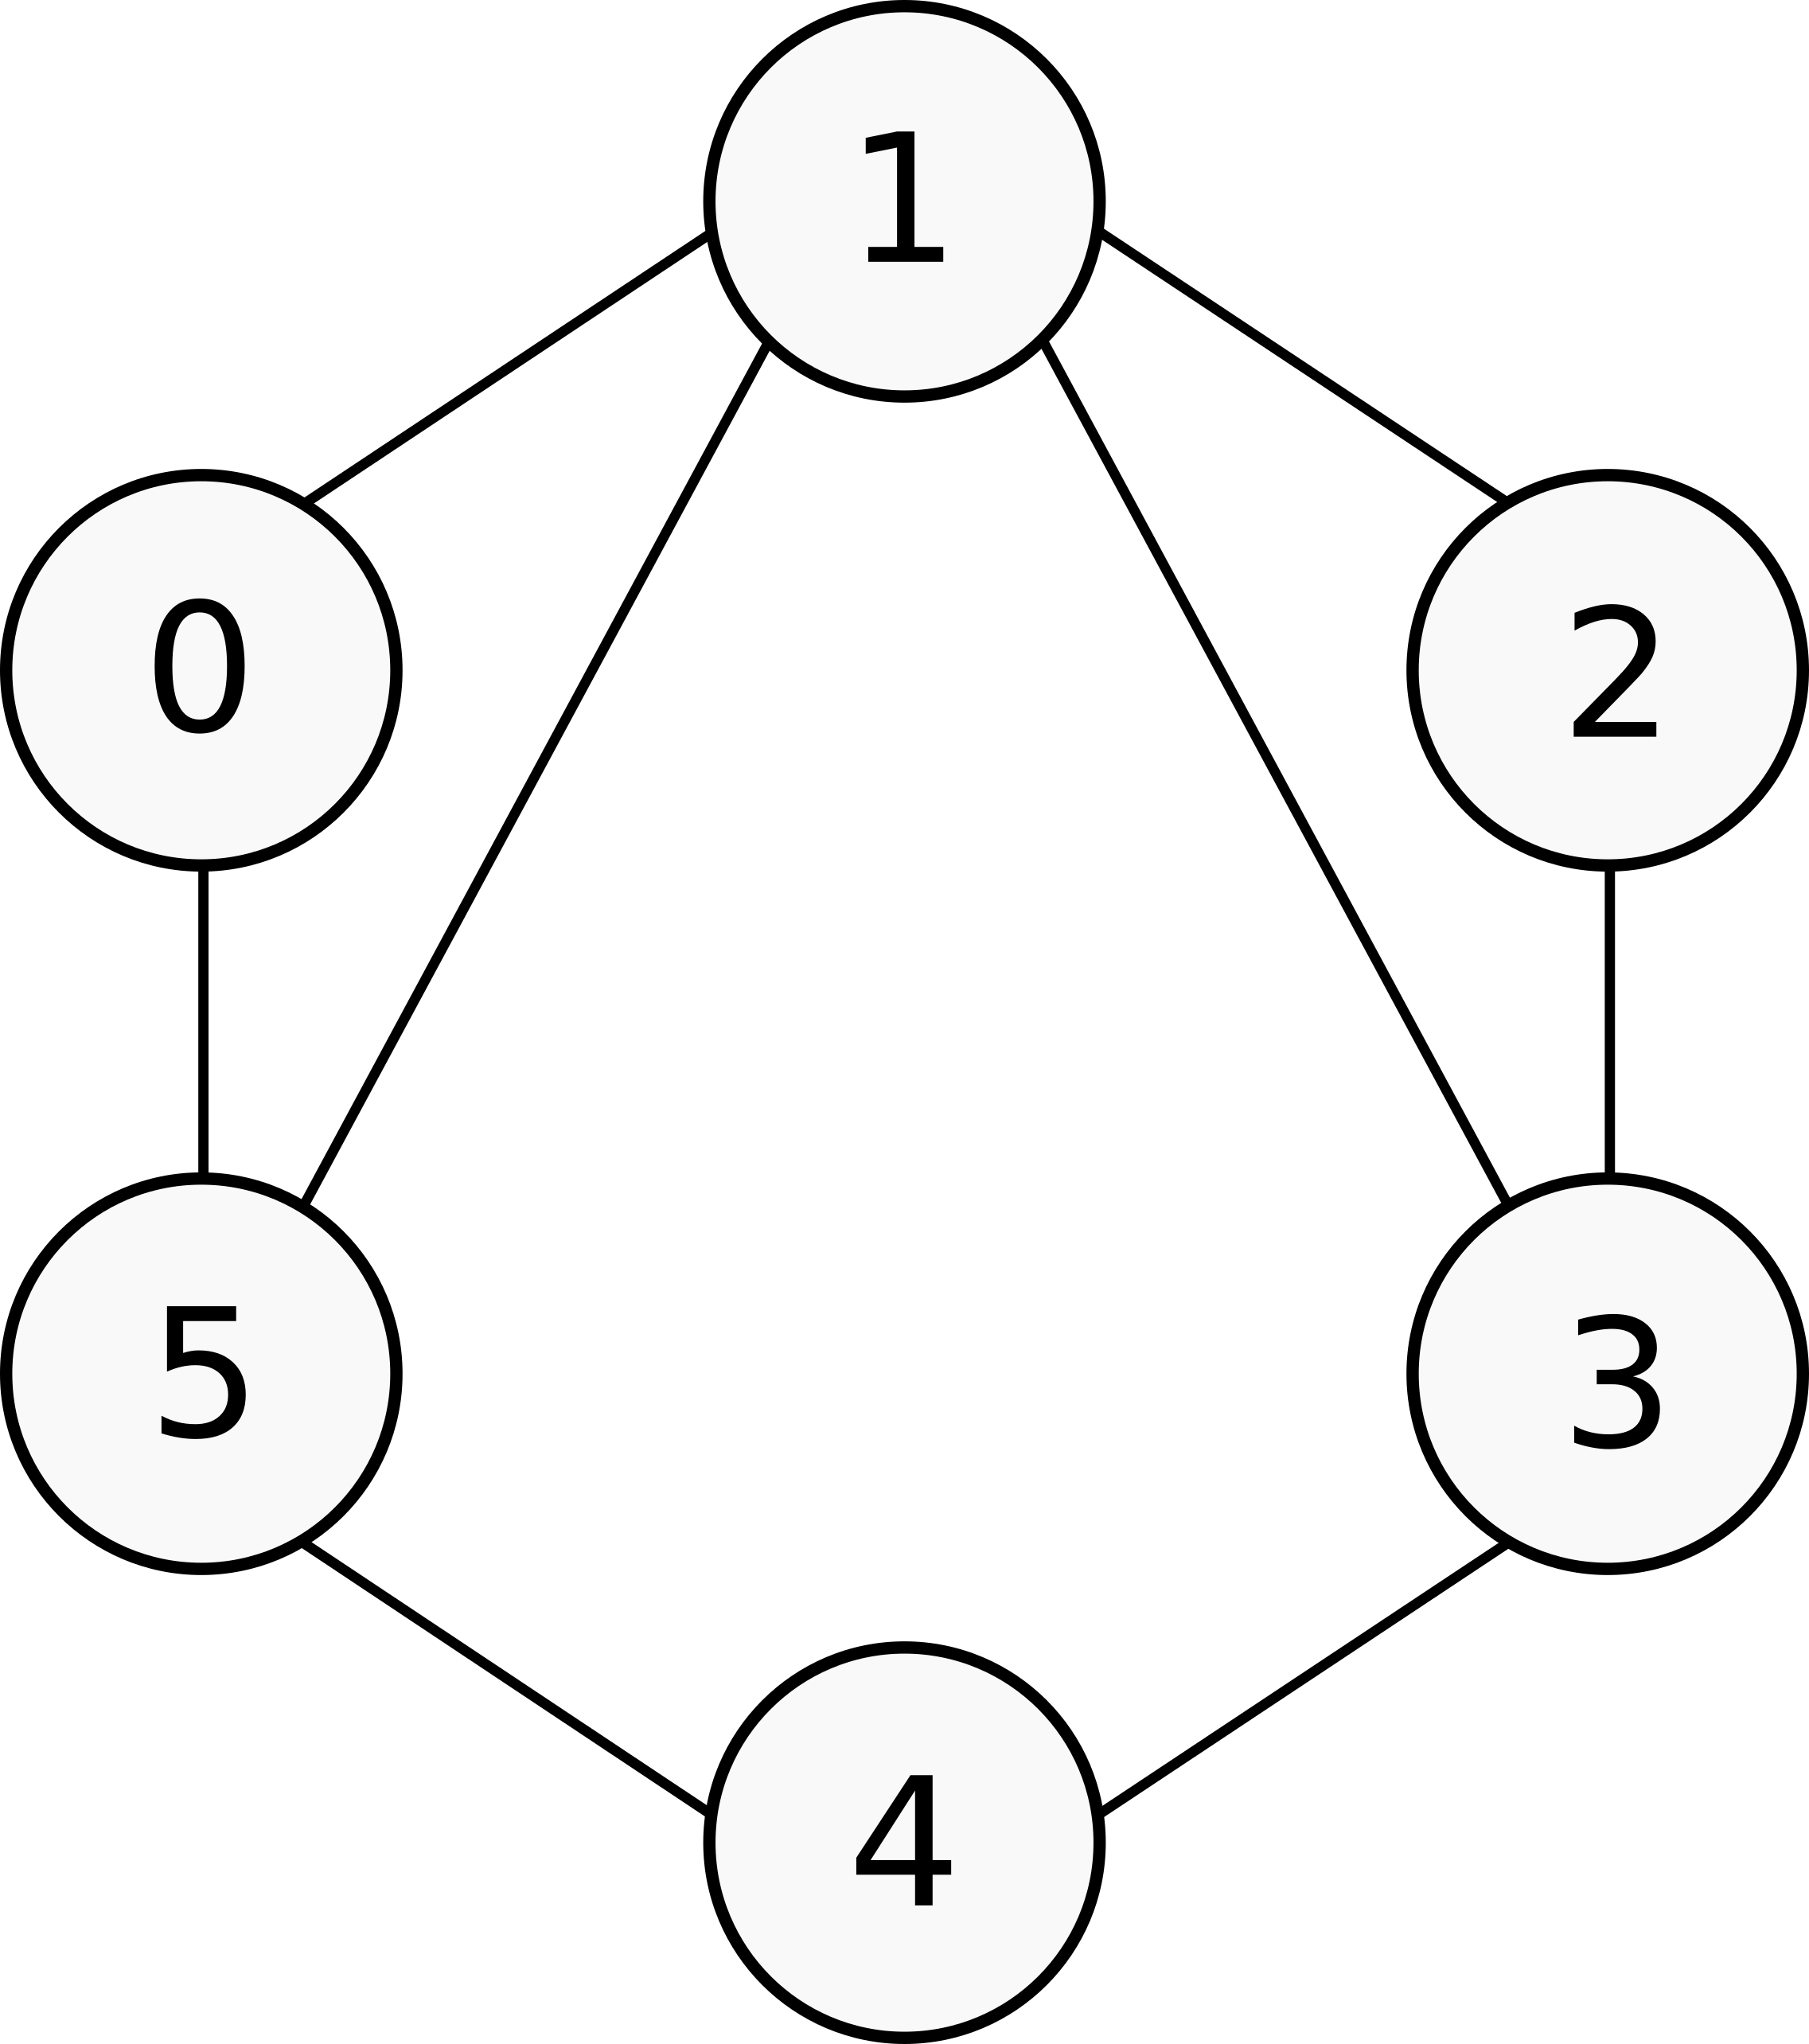
\includegraphics[width=0.50000\textwidth]{img/matriceGrafo_es.png}\\[2\baselineskip]

\begin{enumerate}
\def\labelenumi{\alph{enumi}.}

\item
  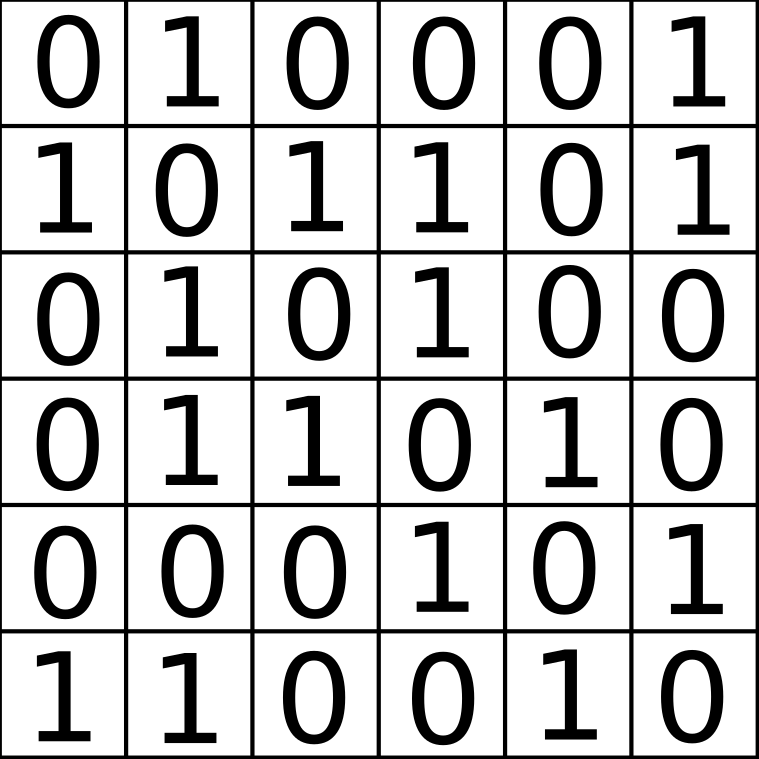
\includegraphics[width=0.30000\textwidth]{img/matriceGrafo_es_sol1.png}
\item
  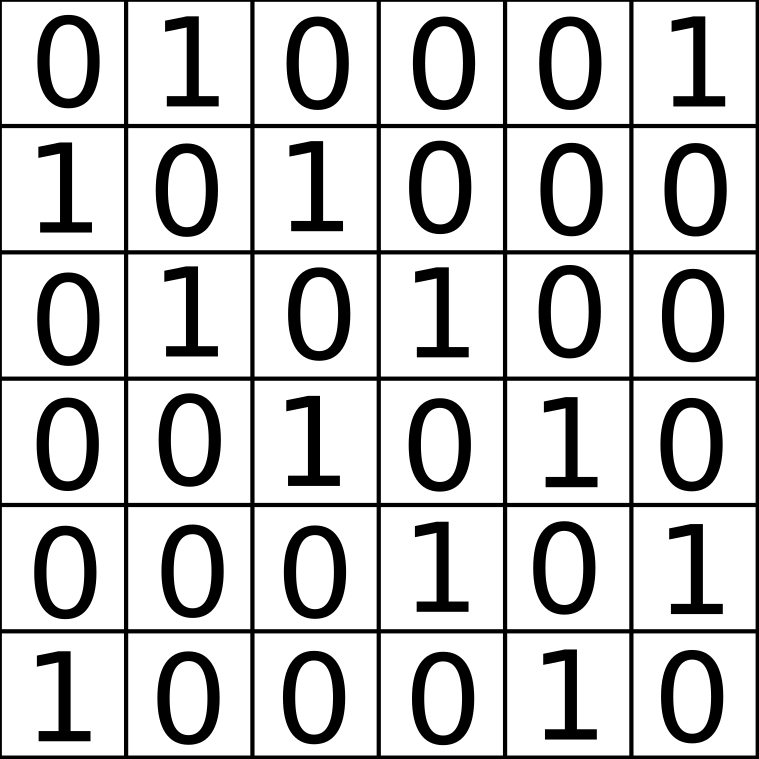
\includegraphics[width=0.30000\textwidth]{img/matriceGrafo_es_sol2.png}
\item
  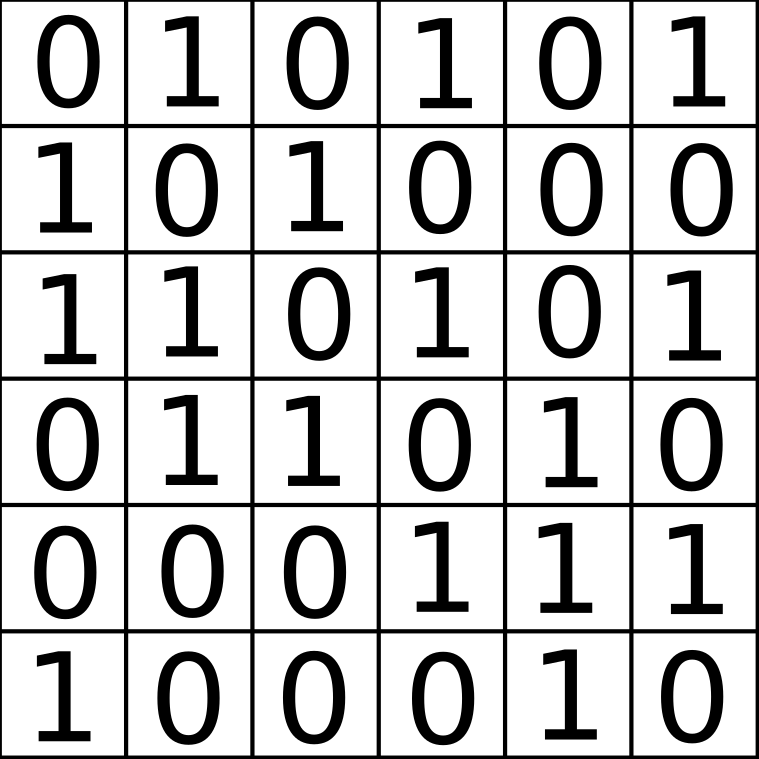
\includegraphics[width=0.30000\textwidth]{img/matriceGrafo_es_sol3.png}
\end{enumerate}

\end{enumerate}


\chapter{Sfruttare il grafo}

Ora che abbiamo visto come creare un grafo in tempo reale durante il gioco, possiamo chiederci come sfruttarlo. Dall'algoritmo boustrophedon abbiamo già imparato come garantire una copertura completa del labirinto. Ora vediamo come usare il grafo generato da \texttt{gioca\_tuki\_generagrafo.c} per trovare un percorso per raggiungere un vertice tra quelli già esplorati.\\

Si immagini di aver già esplorato una parte del labirinto e di voler tornare a un punto specifico (cella bersaglio). Il Boustrophedon ci ha insegnato che dobbiamo camminare all'indietro fino a quando non ci imbattiamo nella cella bersaglio. Questo però significa anche sprecare molti turni di gioco e aumentare la probabilità che l'agent venga catturato dal fantasma. C'è un modo più efficiente per tornare indietro?\\
Ovviamente si possono calcolare tutti i possibili percorsi seguendo gli archi e i vertici fino a raggiungere la cella bersaglio e memorizzare la lunghezza di ciascuno. Al termine si può selezionare il percorso più corto.\\
Sfortunatamente questo metodo richiede un numero enorme di passaggi di calcolo per trovare la soluzione ottimale perché deve testare tutte le possibili combinazioni di vertici collegati tra loro.\\
Il numero di passaggi computazionali richiesti da questo algoritmo aumenta esponenzialmente con l'input, in questo caso, il numero di vertici e archi.\\
Ciò significa che questo algoritmo è adatto a grafi molto piccoli, ma, se i vertici iniziano a crescere, impiega sempre più tempo.

La cattiva notizia è che non esistono tecniche matematiche per ridurre effettivamente la complessità di questo metodo. La buona notizia è che possiamo usare una funzione \emph{euristica} per aiutarci.

\section{Algoritmo A*}

La nostra implementazione dell'algoritmo Astar è riportata nel codice seguente ed è ovviamente presentata nella libreria \\\texttt{libagri}.\\
L'algoritmo Astar (A*) sfrutta due concetti diversi: la distanza misurata e la distanza stimata tra due vertici. Per trovare il percorso da un vertice iniziale a quello bersaglio, l'algoritmo A* utilizza due funzioni: una denominata \emph{esatta} e l'altra detta \emph{euristica}.

\begin{figure}
  \centering
  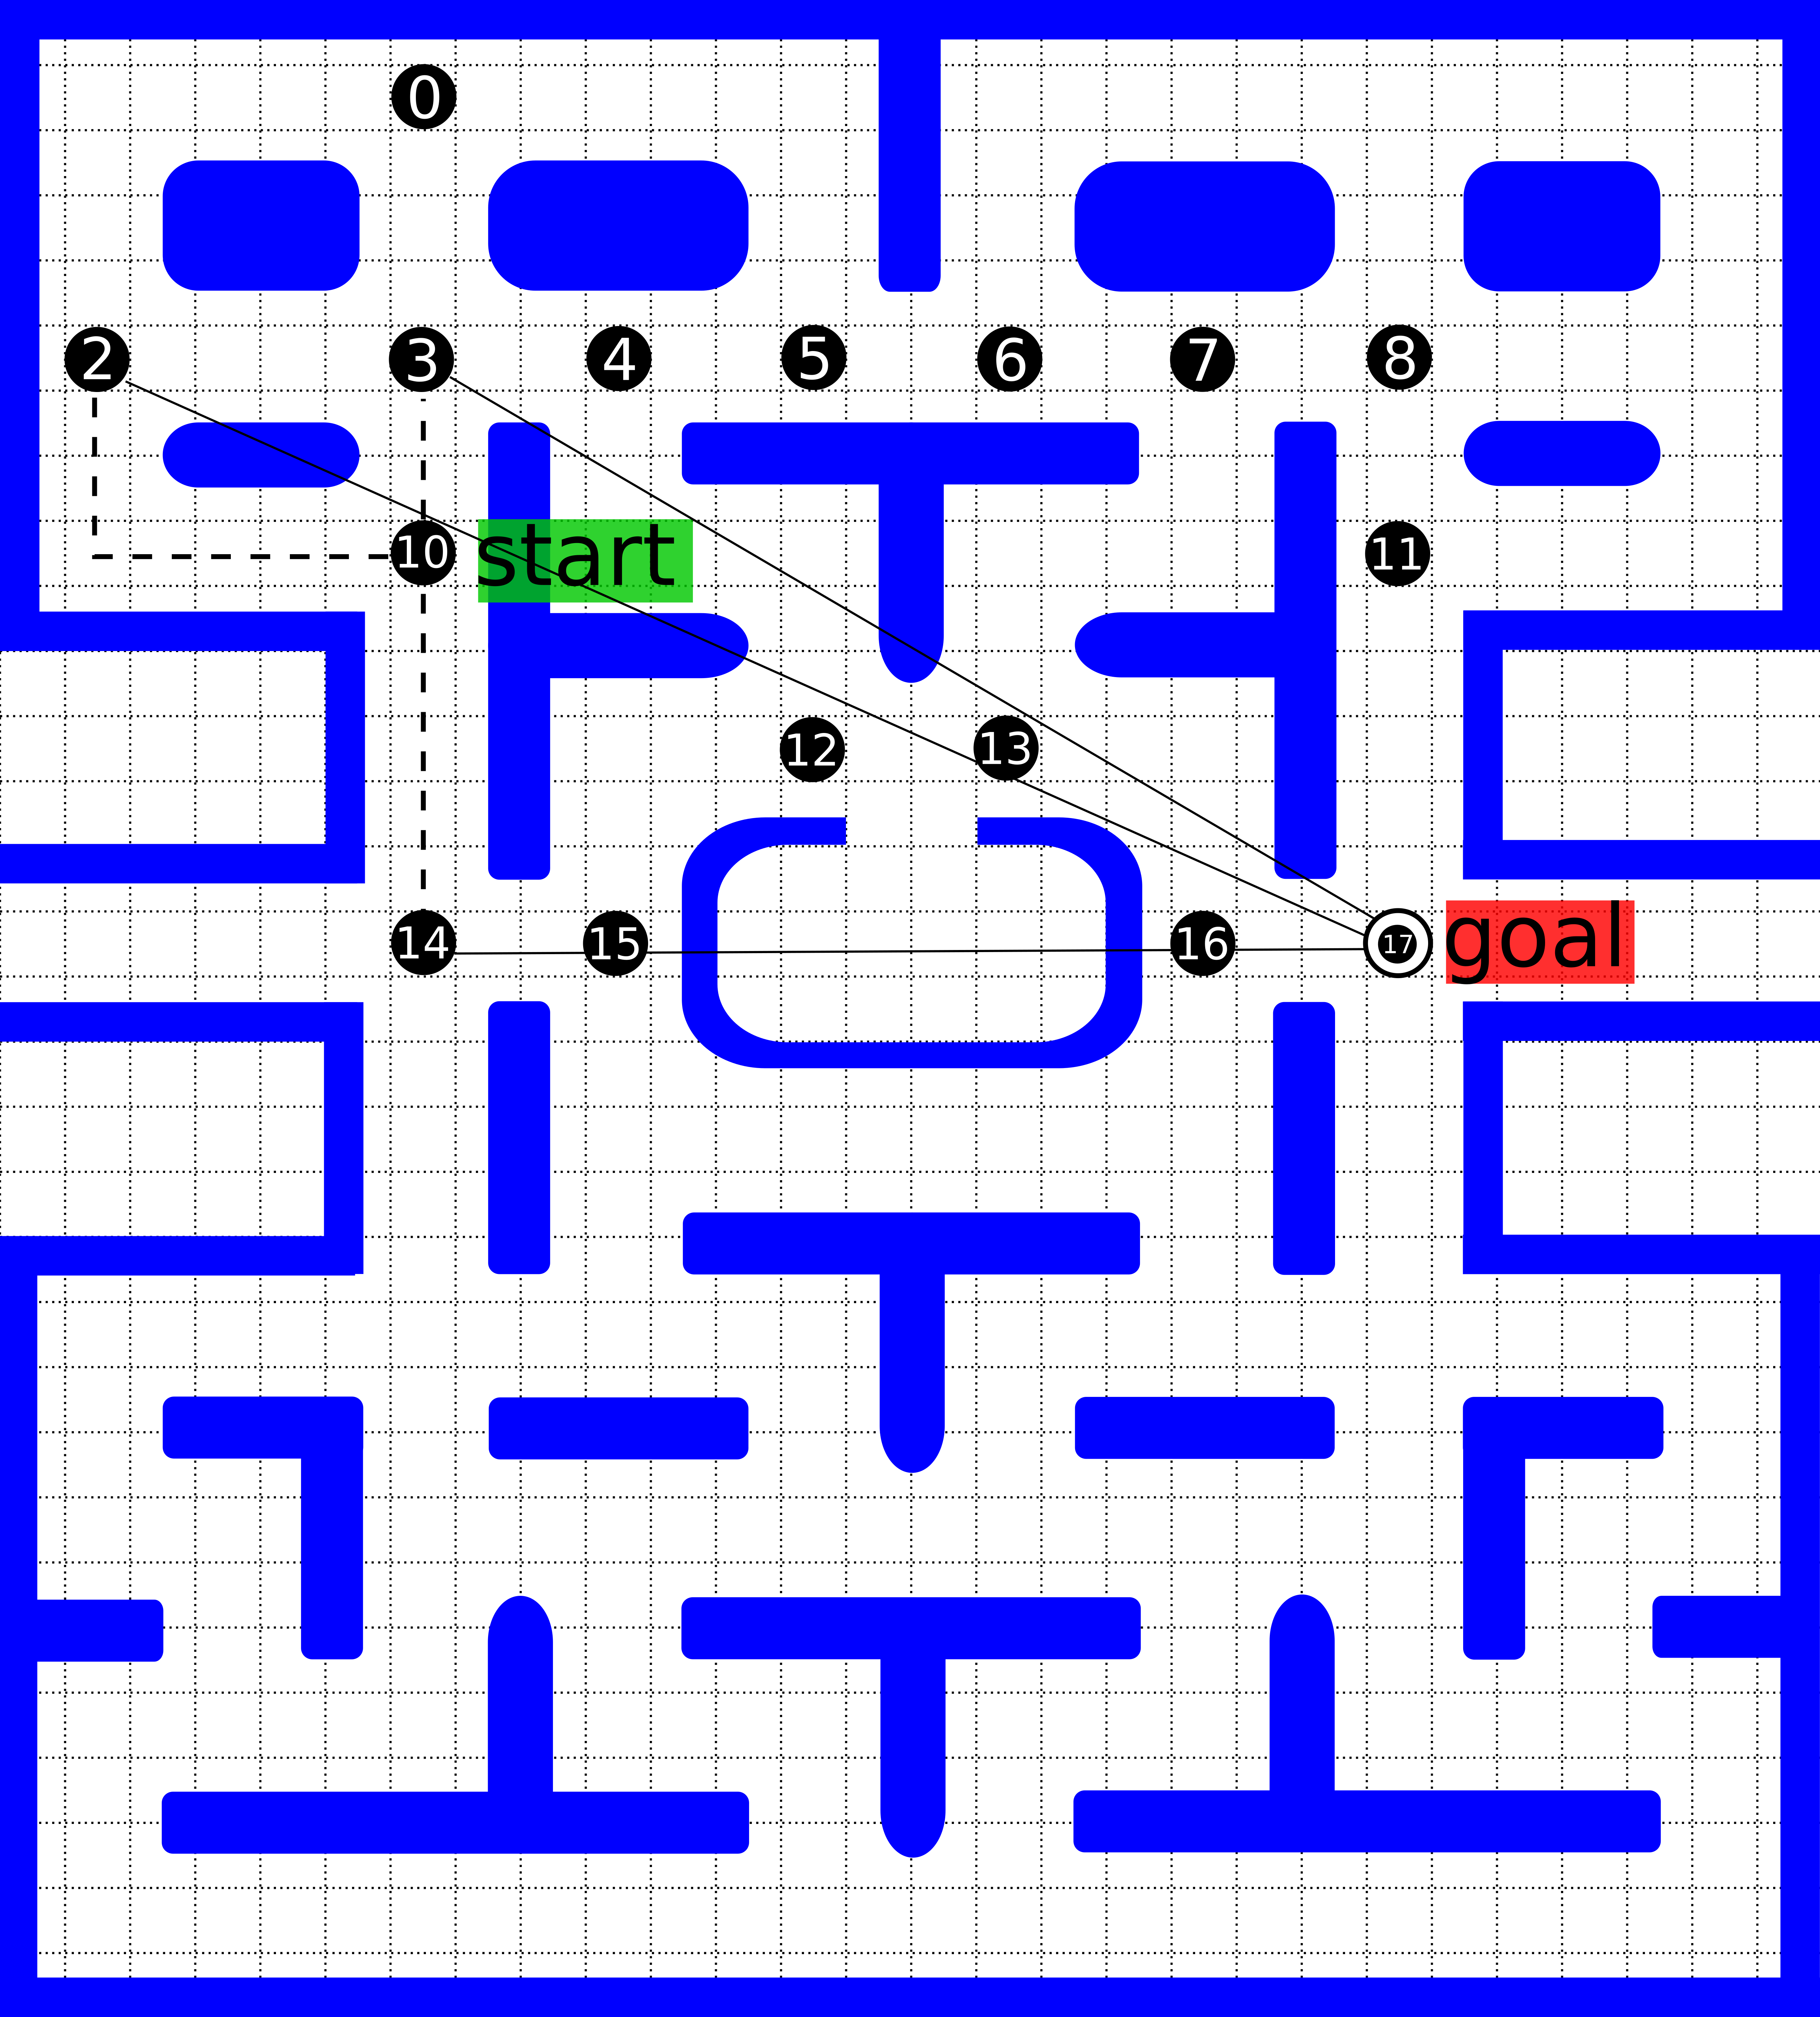
\includegraphics[width=0.55000\textwidth]{img/astar.png}
  \caption{Rappresentazione di A* per la ricerca del percorso dal vertice 10 al 17}
  \label{percorsoAStar1017}
\end{figure}



L'idea di base dell'algoritmo è quella di evitare di valutare tutti i possibili percorsi e concentrarsi principalmente su quelli più promettenti, ovvero i percorsi che \emph{sembrano} i più brevi.

Per spiegare l'algoritmo diamo un'occhiata alla figura \ref{percorsoAStar1017}. Pac-Man deve passare dal vertice $10$ al vertice $17$. Il primo passo di A* è creare una coda prioritaria e riempirla con i vertici vicini dell'attuale vertice, che alla prima iterazione è $10$.

Una coda prioritaria è una specifica struttura dati, per esempio una lista collegata o uno stack, per memorizzare degli elementi ai quali è associata una etichetta di priorità.

La priorità nella coda dipende dalla distanza stimata dei vertici dall'obiettivo (cioè il vertice $17$).\\
La distanza stimata di ciascun vicino si ottiene sommando alla distanza esatta dal vertice corrente la distanza euristica, che, in questo caso, corrisponde alla distanza cartesiana dal vertice obiettivo.\\
La distanza esatta è il numero di celle che separano un vertice dall'altro, ad esempio la distanza tra i vertici $10$ e $2$ è $7$, la distanza tra i vertici $10$ e $3$ è $2$ e la distanza tra i vertici $10$ e $14$ è $5$.\\
Si presti attenzione che in questa specifica implementazione non stiamo considerando le celle occupate dai vertici stessi, nel calcolo della distanza esatta.\\
Le distanze cartesiane dei vertici $2$, $3$ e $14$ dal vertice goal ($17$) sono rispettivamente $22$, $17$ e $15$. Di conseguenza, le loro distanze stimate risultano $7+22=29$ per il vertice $2$, $2+17=19$ per il $3$ e $5+15=20$ per il $14$.\\
Il vertice $3$ è il primo nella coda prioritaria, in quanto la sua distanza stimata è la minore, seguito da $14$ e $2$.\\
Una volta riempita la coda, A* ripeterà nuovamente l'iterazione selezionando il primo vertice nella coda prioritaria, ovvero il vertice $3$, come vertice corrente.\\
Ora che $3$ è il vertice corrente, la procedura viene ripetuta considerando i vicini del vertice $3$ che sono $2$, $0$ e $4$. Seguendo questo metodo, il percorso da $10$ a $17$ è dato dalla seguente sequenza: $3$, $4$, $5$, $6$, $7$, $8$, $11$ e $17$.

\subsection{A* in C}

Per capire l'algoritmo A* seguiamo cosa succede dopo una chiamata alla nostra specifica implementazione dell'algoritmo:

\begin{spacing}{0.9}
  \begin{small}
\begin{tcolorbox}
\begin{verbatim}
agri_Via p = agri_astar
(10, 17, grafo, &distanza, &euristica,34)
\end{verbatim}
    \end{tcolorbox}
  \end{small}
\end{spacing}

Il vertice di partenza $10$ viene inserito nell'elenco di priorità candidati , come si può vedere nel commento A-1.\\
Da A-1 segue un ciclo while che termina quando non ci sono più candidati o quando l'obiettivo (vertice $17$) è stato raggiunto. Ad ogni iterazione viene estratto (pop) il vertice in cima alla lista, ovvero il vertice che ha la priorità più alta, ovvero la distanza più breve dall'obiettivo. Alla prima iterazione nell'elenco è presente solo il vertice di partenza, quindi l'operazione pop lo estrarrà dalla coda, lasciandola vuota.\\
In A-2 viene controllato se il vertice corrente e quello obiettivo corrispondono perché in tale situazione le iterazioni devono arrestarsi e deve essere restituito il percorso. Torneremo su questo punto più tardi.\\
In A-3 vengono analizzati i vicini del vertice $10$ e la distanza dal vertice $17$ viene calcolata per ciascuno di essi utilizzando sia la distanza esatta che quella euristica. Si noti che la funzione \texttt{agri\_astar} accetta il puntatore alle funzioni che si desidera implementare per calcolare le distanze esatta ed euristica.\\
Ora siamo al punto critico poiché l'algoritmo deve decidere quale dei vertici vicini aggiungere alla coda di priorità. Al punto A-4 sono stati inizializzati due array: \texttt{gscore} che contiene la distanza esatta (misurata in unità di cella) di ciascun vertice dal vertice iniziale e \texttt{fscore} che è \texttt{gscore} sommato alla distanza euristica stimata del vertice dall'obiettivo.\\
Al momento dell'inizializzazione ogni elemento dei due array è impostato su infinito (9999) ad eccezione degli elementi corrispondenti al vertice iniziale che sono impostati rispettivamente su $0$ e sulla distanza cartesiana.\\
Quindi, per il vertice iniziale, avremo \texttt{gscore {[}10{]} = 0} e \texttt{fscore {[}10{]} = 16} . In A-5 tutti i vertici adiacenti a quello iniziale soddisfano la \texttt{if-clause} perché il loro \texttt{gscore} è infinito e tutti saranno inseriti nella coda di priorità e il loro \texttt{gscore} verrà aggiornato con la loro distanza dal vertice iniziale, mentre il loro \texttt{fscore} verrà impostato sul loro \texttt{gscore} sommato alla distanza cartesiana dal vertice obiettivo.\\
I vertici $2$, $3$ e $14$ vengono quindi inseriti nella coda di priorità con il $3$ in cima alla coda. Per ognuno dei vertici appena inseriti in coda, viene memorizzato, al rispettivo indice dell'array chiamato \texttt{precedente}, l'indice del vertice corrente, ovvero il $10$. In pratica l'array \texttt{precedente} serve per ricostruire la sequenza dei vertici a ritroso una volta che si è raggiunto il vertice obiettivo.\\
Alla successiva iterazione, $10$ non è più il vertice corrente, ma lo diventa il vertice $3$ a causa dell'operazione pop al punto A-6. Il blocco \texttt{if} nel punto A-2 non viene eseguito perché il vertice obiettivo è il $17$ ed è diverso da $3$. Il codice salta quindi in A-3 dove sono considerati i vicini del vertice $3$, che sono: $2$, $0$, $4$ e $10$.\\
A questo punto siamo di nuovo in A-5 dove esiste la possibilità che il \texttt{gscore} del vertice $2$ possa essere aggiornato. In effetti è possibile che il percorso che porta al vertice $2$ passando per il $3$ sia più corto di quello che lo connette direttamente al $10$.\\

Questo pezzo di codice è molto importante nei grafi in cui la lunghezza degli archi è molto diversa dalla distanza cartesiana tra i vertici, comunque non gioca un ruolo importante nel labirinto di Pac-Man.\\

L'algoritmo procede in questo modo fino a quando il vertice $17$ risulta essere uno dei vicini del vertice corrente e viene quindi creato il percorso completo.\\
Alla fine la \texttt{if-clause} nel punto A-2 è vera e il blocco di codice viene eseguito. Nel loop A-7 tutti i vertici del percorso vengono scorsi all'indietro assegnando \texttt{corrente = precedente {[}corrente{]}} .\\
L'elenco dei vertici viene memorizzato nello heap e un puntatore al primo byte dell'array precedente viene restituito al chiamante della funzione.

\begin{spacing}{0.85}
  \begin{small}
\begin{tcolorbox}
\begin{verbatim}
agri_Via agri_astar(int start, int goal,
		    agri_Vertex * agri_Vertices_Colligati,
		    double (*spatium)(int ab, int ad),
		    double (*euristica)(int ab, int ad),
		    int nmembri
		    )
{
  if(start==goal)
    {
      return 0;
    }
  double fscore[nmembri];
  double gscore[nmembri];
  int precedente[nmembri];
  
  //Nodi in valutazione per il path da start a goal
  Ordo candidati = 0;
  
  /* A-4 */
  for(int i=0;i<nmembri;i++)
    {
      fscore[i] = INFINITO;
      gscore[i] = INFINITO;
    }
  gscore[start] = 0;
  fscore[start]=euristica(start,goal);
  
  Ordo_insero_nodus
    (&candidati,start,(1./fscore[start]));
  
  /* A-1 */
  while(candidati != 0)
    {
      fflush(stdout);
      /* A-6 */
      int corrente = Ordo_pop(&candidati);
      
      /* A-2 */
      /* Arrivato al nodus goal torna il cammino */
      if(corrente == goal)
        {
          fflush(stdout);
          int i = 0;
          int aux[nmembri];

          /* A-7 */
          do{
            aux[i]=corrente;
            corrente=precedente[corrente];
            i++;
          } while(corrente != start);
\end{verbatim}
    \end{tcolorbox}
  \end{small}
\end{spacing}



\begin{spacing}{0.85}
  \begin{small}
\begin{tcolorbox}
\begin{verbatim}	  
          agri_Via percorso = malloc((i+1)*sizeof(int));
	  
          int j =0 ;
          for(int k = i-1;k >=0 ;k--,j++)
            {
              percorso[j] = aux[k];
            }
          // Segnale di fine percorso
          percorso[j]=-1;
          return percorso;
        }
     
      /* A-3 */
      /* Nel labirinto di Pac-Man ci sono al massimo 
      4 vicini */
      int vicino[PORTE];
      for(int i=0; i<PORTE; i++)
        {
          vicino[i] = 
          agri_Vertices_Colligati[corrente].ianua[i];
        }
      
      for(int i =0; i<PORTE; i++)
        {
          int iv = vicino[i];
	  
          /* ogni nodus è predisposto per 4 vicini, 
             ma molti nodi ne hanno solo 3*/
          if(iv == -1)continue;
	  
          double d =  spatium(corrente, iv);
          double tent_gscore = gscore[corrente]+d;
	  
          /* A-5 */
          if(tent_gscore <= gscore[iv])
            {
              /* Trovato cammino migliore a questo nodus 
                 passando per corrente*/
              precedente[iv] = corrente;
              gscore[iv] = tent_gscore;
              fscore[iv] = gscore[iv]+euristica(iv, goal);
	      
              Ordo_insero_nodus
              (&candidati,iv, ( 1./fscore[iv]));
	      
              fflush(stdout);
            }
        }
    }
  return 0;
}
\end{verbatim}
    \end{tcolorbox}
  \end{small}
\end{spacing}


\section[L'algoritmo A*]{Navigazione nel grafo esplorato usando l'algoritmo A *}

L'algoritmo A* combinato con la rappresentazione a grafo del labirinto Pac-Man offre l'opportunità di creare un agent in grado di muoversi in modo deterministico all'interno del labirinto.\\

L'idea è quella di codificare un agent che esplori il labirinto per creare il grafo e nel frattempo usi il grafo creato per guidare se stesso nell'esplorazione.

\subsection{Specifiche dell'agent}

Chiediamo semplicemente all'agent di tornare periodicamente a un certo punto del labirinto.\\
Gli chiediamo di tornare a un dato vertice dopo aver aggiunto un certo numero di vertici al suo grafo. In altre parole, l'agent deve tornare a casa per pranzo dopo una giornata di lavoro!\\
La scelta di innescare il ritorno dell'agent in base al numero di vertici aggiunti è solo a titolo di esempio di possibili usi dell'A*. Si potrebbero fare diverse scelte come parametro di innesco del ritorno, come ad esempio il tempo di vagabondaggio o il numero di passi (turni di gioco) eseguiti.\\
Ci chiediamo però cosa succede se Pac-Man incontra un fantasma. In questo caso, chiediamo all'agent di ``sospendere'' la sua esplorazione o di sospendere il suo ritorno a casa e fuggire dal fantasma fino a quando il fantasma non è più nelle vicinanze. Queste due semplici regole saranno la logica che guiderà il nuovo agent.

\subsection{Implementazione}

Per implementare la specifica dell'agent, sono necessari i seguenti passaggi:

\begin{enumerate}
\item
  creare il grafo durante il vagabondaggio di Pac-Man nel labirinto
\item
  contare i nuovi vertici aggiunti al grafo
\item
  chiamare l'algoritmo A* quando è stato raggiunto il numero di nuovi vertici aggiunti al grafo
\item
  memorizzare il percorso in memoria come un array di vertici
\item
  trovare la direzione per il prossimo vertice nel percorso restituito
\end{enumerate}

\newpage
\textbf{Passo 1}

\begin{spacing}{0.9}
  \begin{small}
\begin{tcolorbox}
\begin{verbatim}
agri_Colligatio colligatio;
agri_Vertex v_a, v_da;
v_a = agri_Verticem_creo(vertice_a,i,j);
v_da = agri_Verticem_creo(vertice_da,i_da,j_da);

distanze[vertice_da][vertice_a] = longitudo_colligatio;

colligatio.ad = v_a;
colligatio.ab = v_da;
colligatio.longitudo = longitudo_colligatio;
colligatio.meta = direzione_arrivo;
colligatio.discessus = direzione_partenza;
agri_Colligationem_insero(&g, colligatio);
nodo_rilevato = true;
\end{verbatim}
    \end{tcolorbox}
  \end{small}
\end{spacing}

\textbf{Passo 2}

\begin{spacing}{0.9}
  \begin{small}
    \begin{tcolorbox}
\begin{verbatim}
int vertice_a = agri_Verticem_quaero(g,i,j);
if(vertice_a<0)
  {
    vertice_a = vertici_contati;
    vertici_contati++;
    nodi_percorsi++;
  }
\end{verbatim}
  \end{tcolorbox}
    \end{small}
      \end{spacing}

\textbf{Passi 3-4}

\begin{spacing}{0.9}
  \begin{small}
    \begin{tcolorbox}
\begin{verbatim}
/* Il percorso */
static int * percorso_fuga = 0;
/* Copia del percorso */
static int * copia;
...
/* Chiama A* per calcolare il percorso */
percorso_fuga = agri_astar(...);
...
/* Libera lo heap */
if(copia) free(copia);
\end{verbatim}
  \end{tcolorbox}
    \end{small}
      \end{spacing}

\textbf{Passo 5}

\begin{spacing}{0.9}
  \begin{small}
    \begin{tcolorbox}
\begin{verbatim}
/*
  Cerca la direzione per raggungere il 
  prossimo vertice
*/
if(vert_disp[vertice_da].ianua[SINISTRA] ==
   indice_nodo)
  {
    ld = SINISTRA;
  }
if(vert_disp[vertice_da].ianua[DESTRA] ==
   indice_nodo)
  {
    ld = DESTRA;
  }
if(vert_disp[vertice_da].ianua[SU] ==
   indice_nodo)
  {
    ld = SU;
  }
if(vert_disp[vertice_da].ianua[GIU] ==
   indice_nodo)
  {
    ld = GIU;
  }
\end{verbatim}
  \end{tcolorbox}
    \end{small}
      \end{spacing}

Il codice completo è presentato in appendice.

\subsubsection{Compilazione ed esecuzione}

Compilare ed eseguire come indicato nel seguito:

\texttt{
  \newline
\textasciitilde{}/grafi\textbackslash{}\$ ./compila.sh PacMan/gioca\_tuki\_esploraeritorna.c\\ 1 50
}\\

Poi esegui specificando zero fantasmi:

\texttt{
  \newline
  \textasciitilde{}/grafi\textbackslash{}\$ ./tuki5.game 0
  }\\

esegui specificando uno o più fantasmi:

\texttt{
  \newline
  \textasciitilde{}/grafi\textbackslash{}\$ ./tuki5.game 1
  }

\newpage
\section*{Box domande n.4}
\addcontentsline{toc}{section}{Box domande n.4}

\begin{enumerate}
\item Il Pac-Man si trova sul vertice 25 e deve raggiungere il 22. L'agent che lo guida è l'astar. Quale di queste code di priorità è quella giusta?

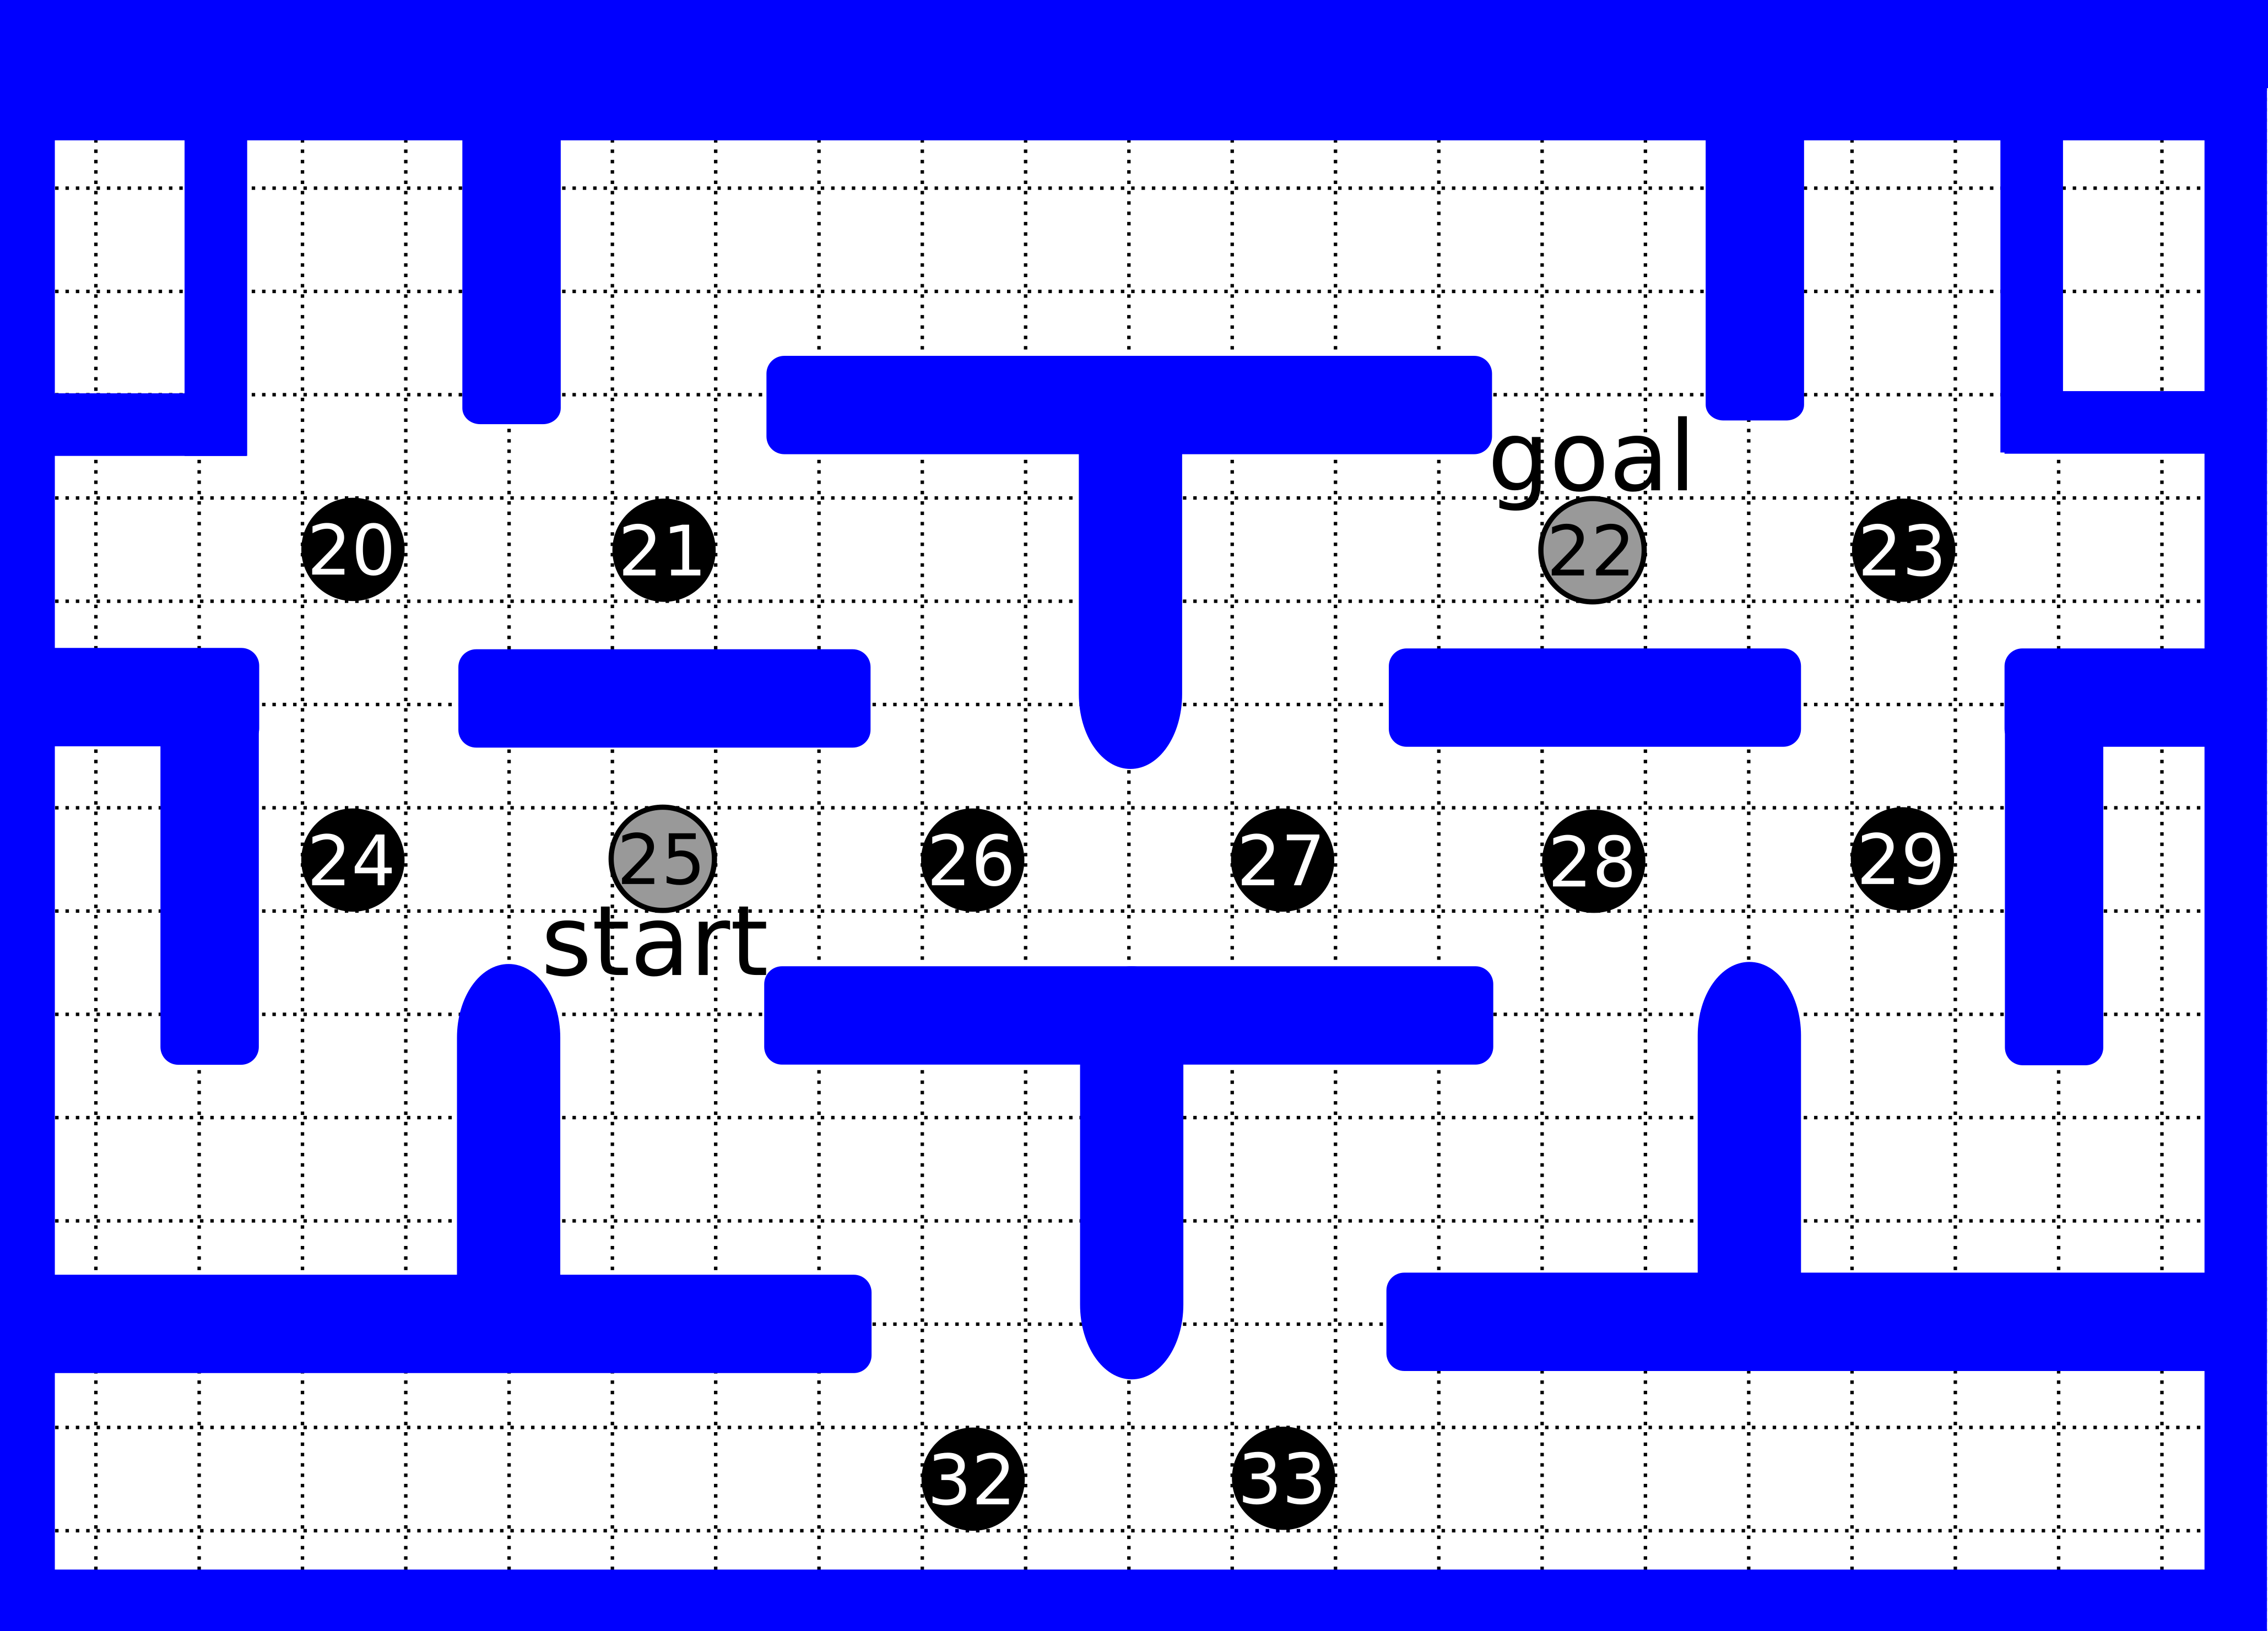
\includegraphics[width=0.70000\textwidth]{img/astar_coda_es.png}\\[2\baselineskip]

\begin{enumerate}
\def\labelenumi{\alph{enumi}.}
\item
  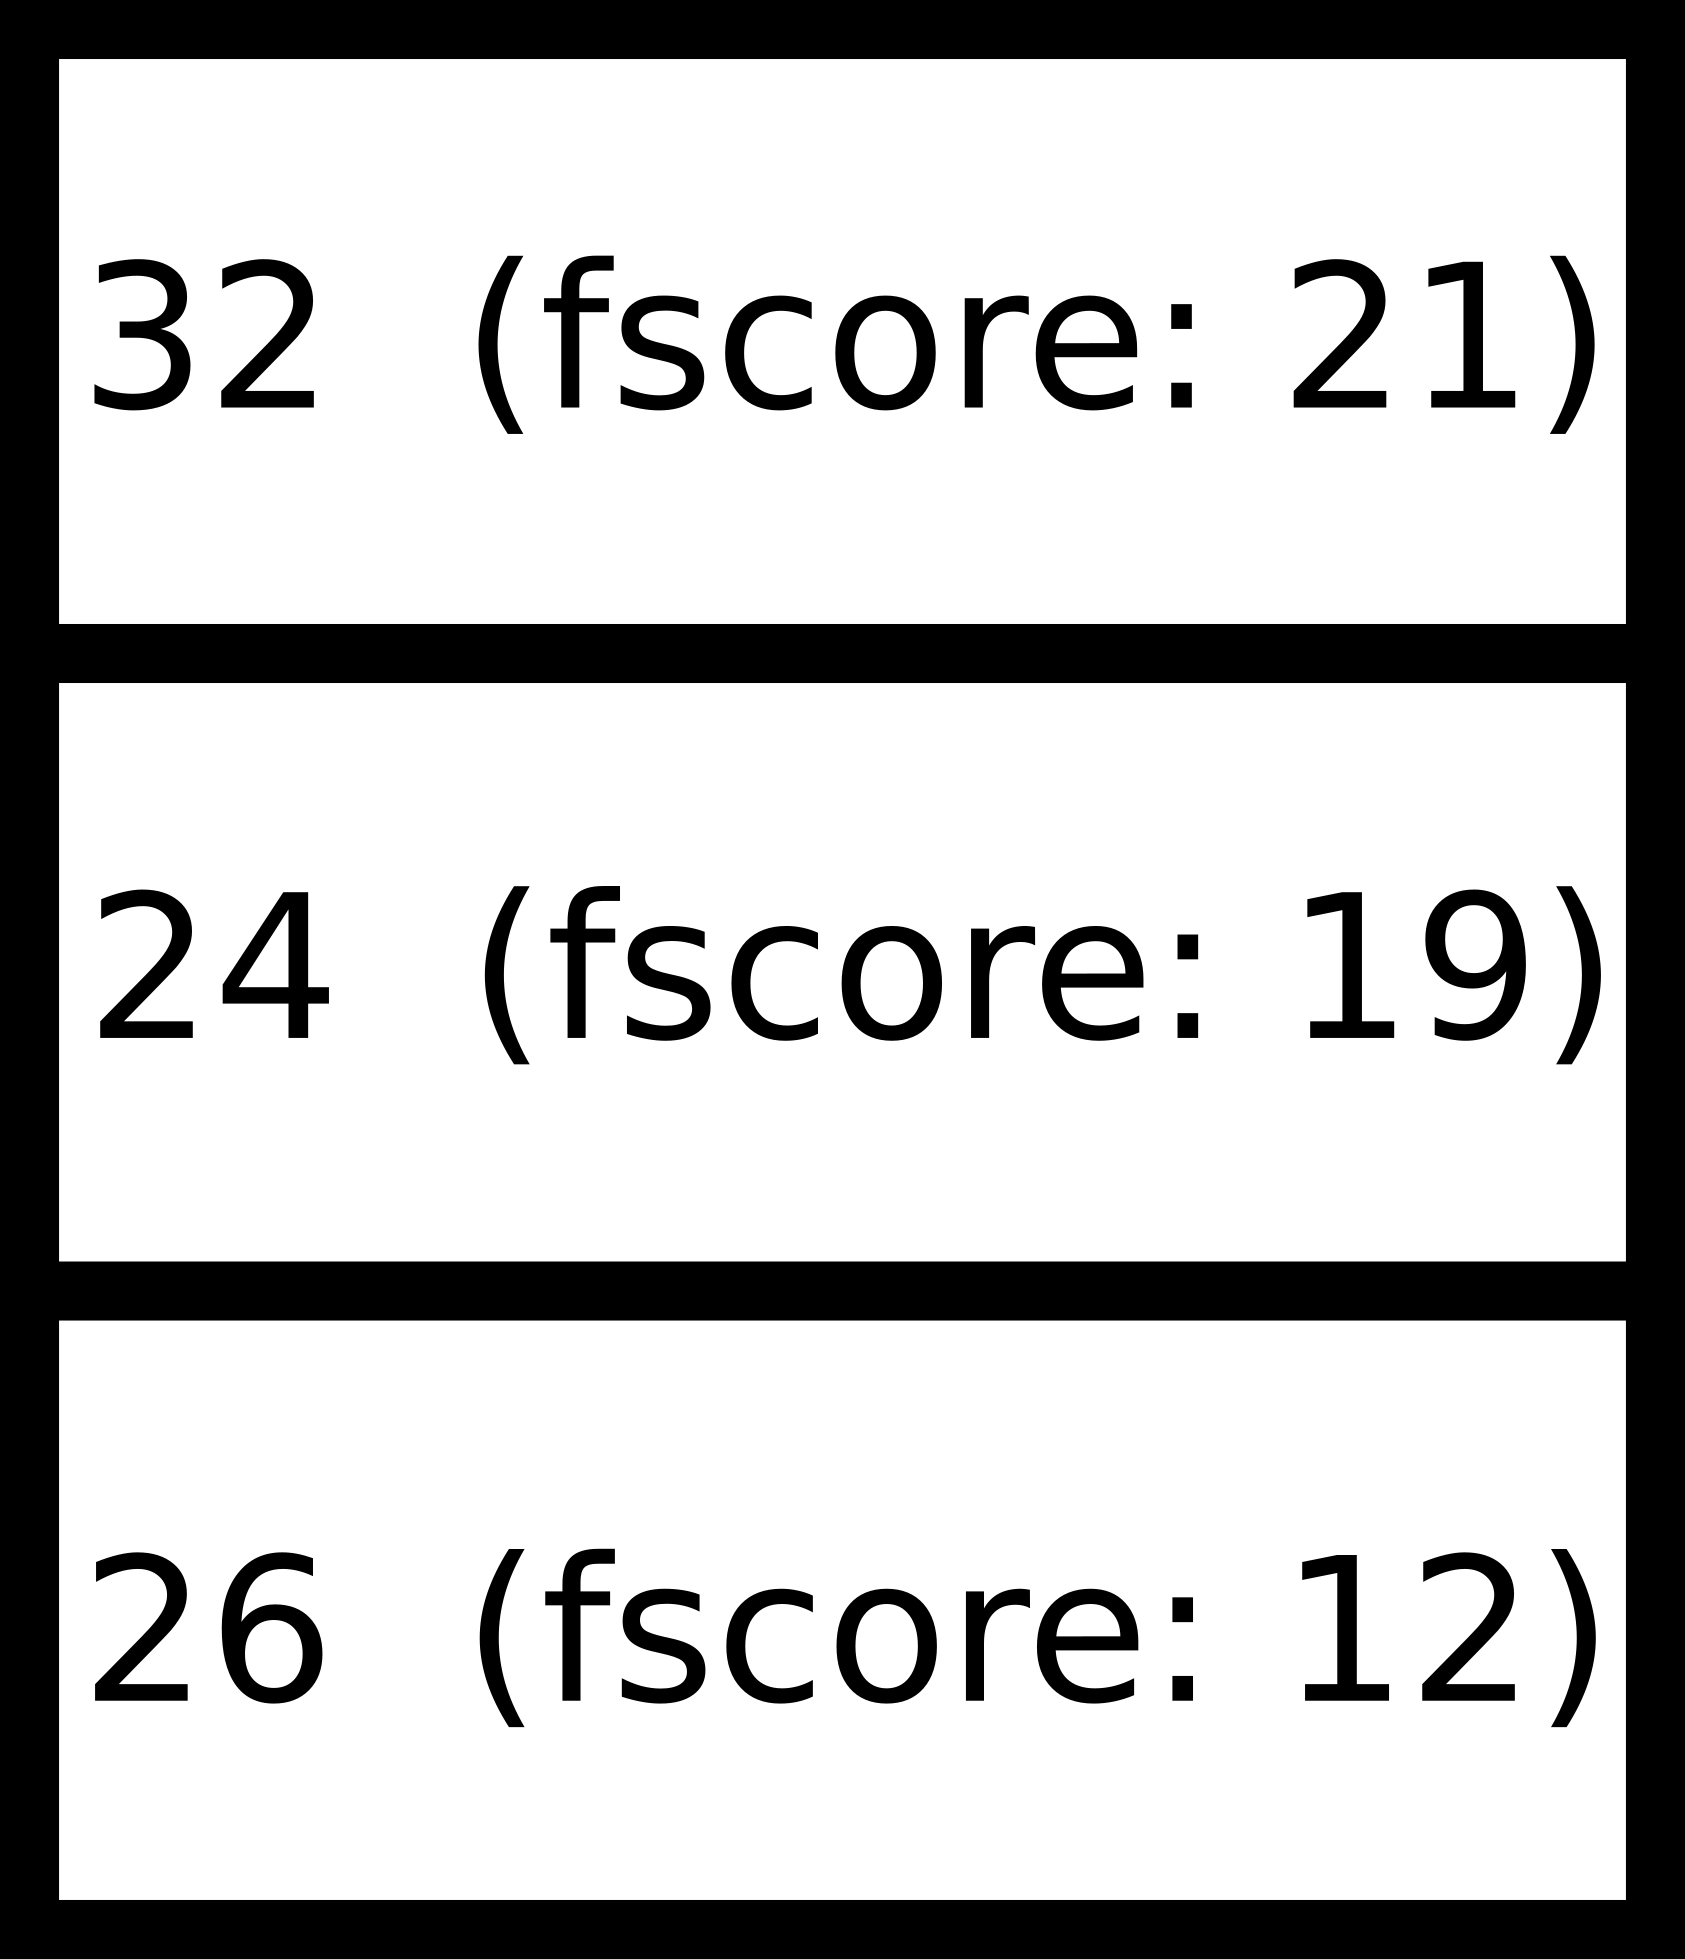
\includegraphics[width=0.30000\textwidth]{img/astar_coda_es_sol1.png}
\item
  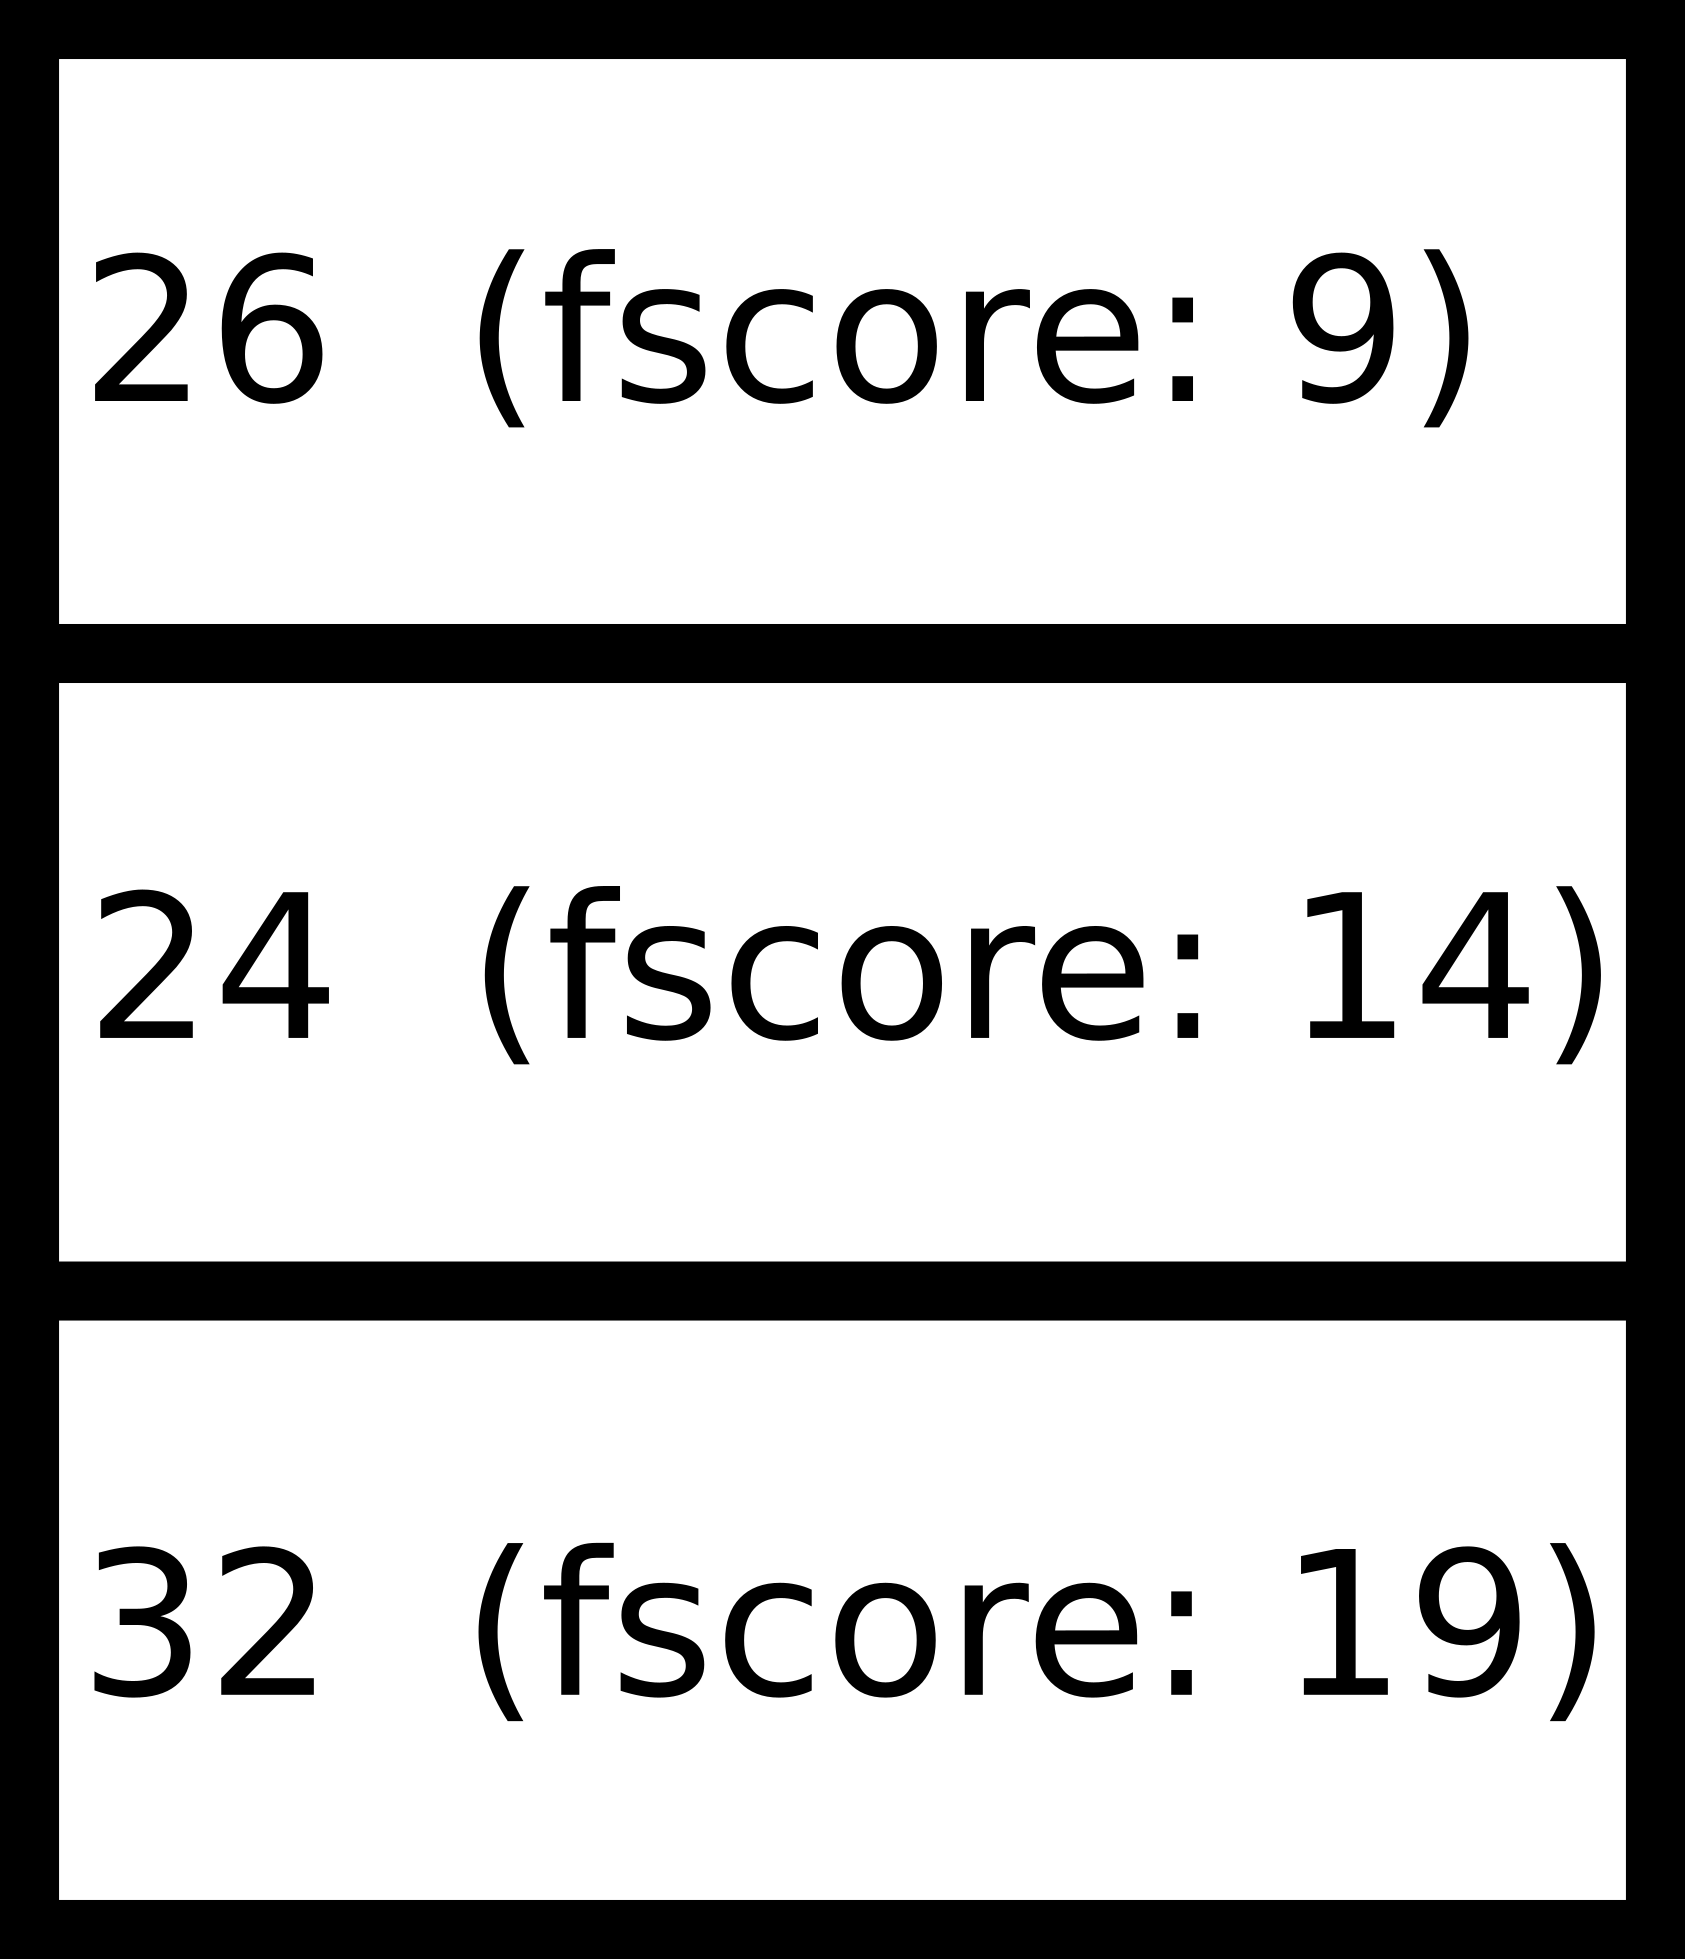
\includegraphics[width=0.30000\textwidth]{img/astar_coda_es_sol2.png}
\item
  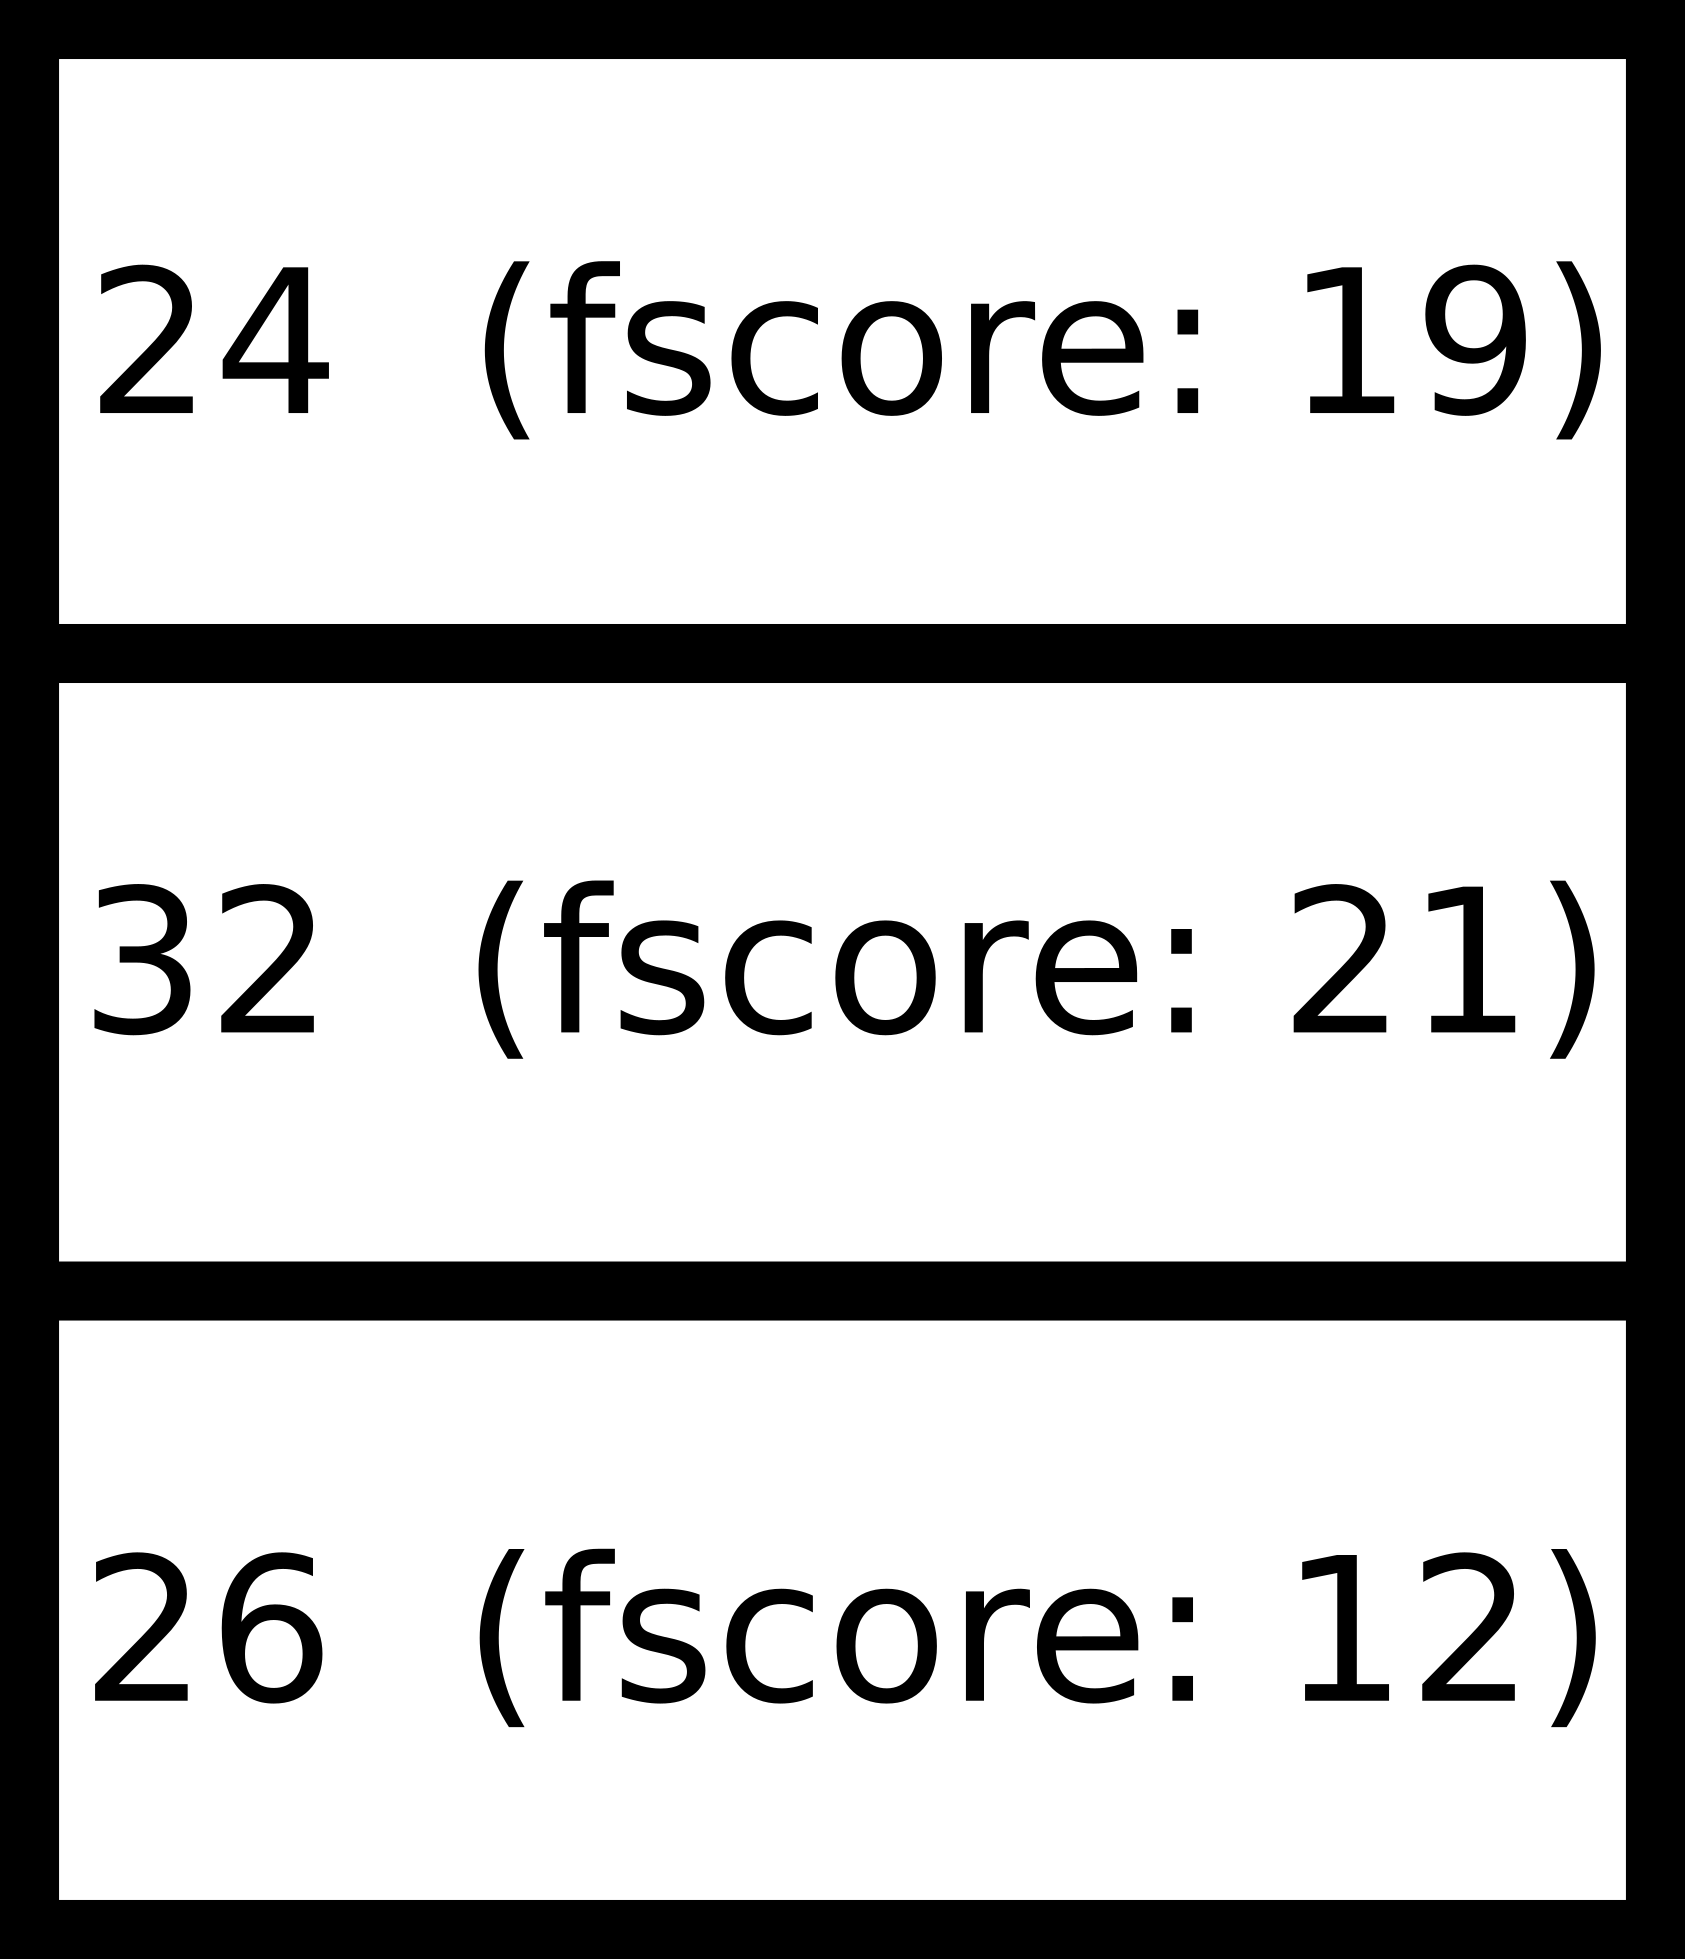
\includegraphics[width=0.30000\textwidth]{img/astar_coda_es_sol3.png}
\end{enumerate}

\item Al termine dell'esecuzione dell'algoritmo astar, cosa contiene l'array precedente?

\begin{enumerate}
\def\labelenumi{\alph{enumi}.}
\item
  La lista di tutti i vertici considerati durante la ricerca del percorso
\item
  I vicini del vertice goal
\item
  Il percorso sub-ottimale restituito dall'algoritmo per raggiungere il vertice goal partendo dal vertice start
\end{enumerate}

\item Cosa contengono gli array \texttt{gscore} e \texttt{fscore}?

\begin{enumerate}
\def\labelenumi{\alph{enumi}.}
\item
  \texttt{gscore}: distanza esatta di ogni vertice dal vertice start\\
  \texttt{fscore}: \texttt{gscore} + distanza cartesiana di ogni vertice dal vertice goal
\item
  \texttt{gscore}: distanza esatta di ogni vertice dal suo precedente\\
  \texttt{fscore}: \texttt{gscore} + distanza esatta do ogni vertice dal vertice goal
\item
  \texttt{gscore}: distanza stimata di ogni vertice dal vertice start\\
  \texttt{fscore}: distanza cartesiana di ogni vertice dal vertice goal
\end{enumerate}

\end{enumerate}

\part{Full Observability}

\chapter{Preparazione del grafo}

In questa sezione cambiamo il paradigma del gioco e assumiamo la osservabilità totale. La piena (full) osservabilità (FO) significa che l'agent ha piena conoscenza della struttura del labirinto nel momento in cui inizia il gioco. Ciò consente all'agent di scegliere una sequenza di vertici per ridurre al minimo la lunghezza del percorso.

È facile intuire che il problema di ridurre al minimo (minimizzare) la lunghezza del percorso ha molte applicazioni pratiche nel mondo reale. Ad esempio è importante in tutte le attività di logistica, come ad esempio nella definizione del percorso degli addetti ai carrelli in un magazzino merci.

\begin{figure}
  \centering
  \begin{subfigure}[b]{0.49\textwidth}
    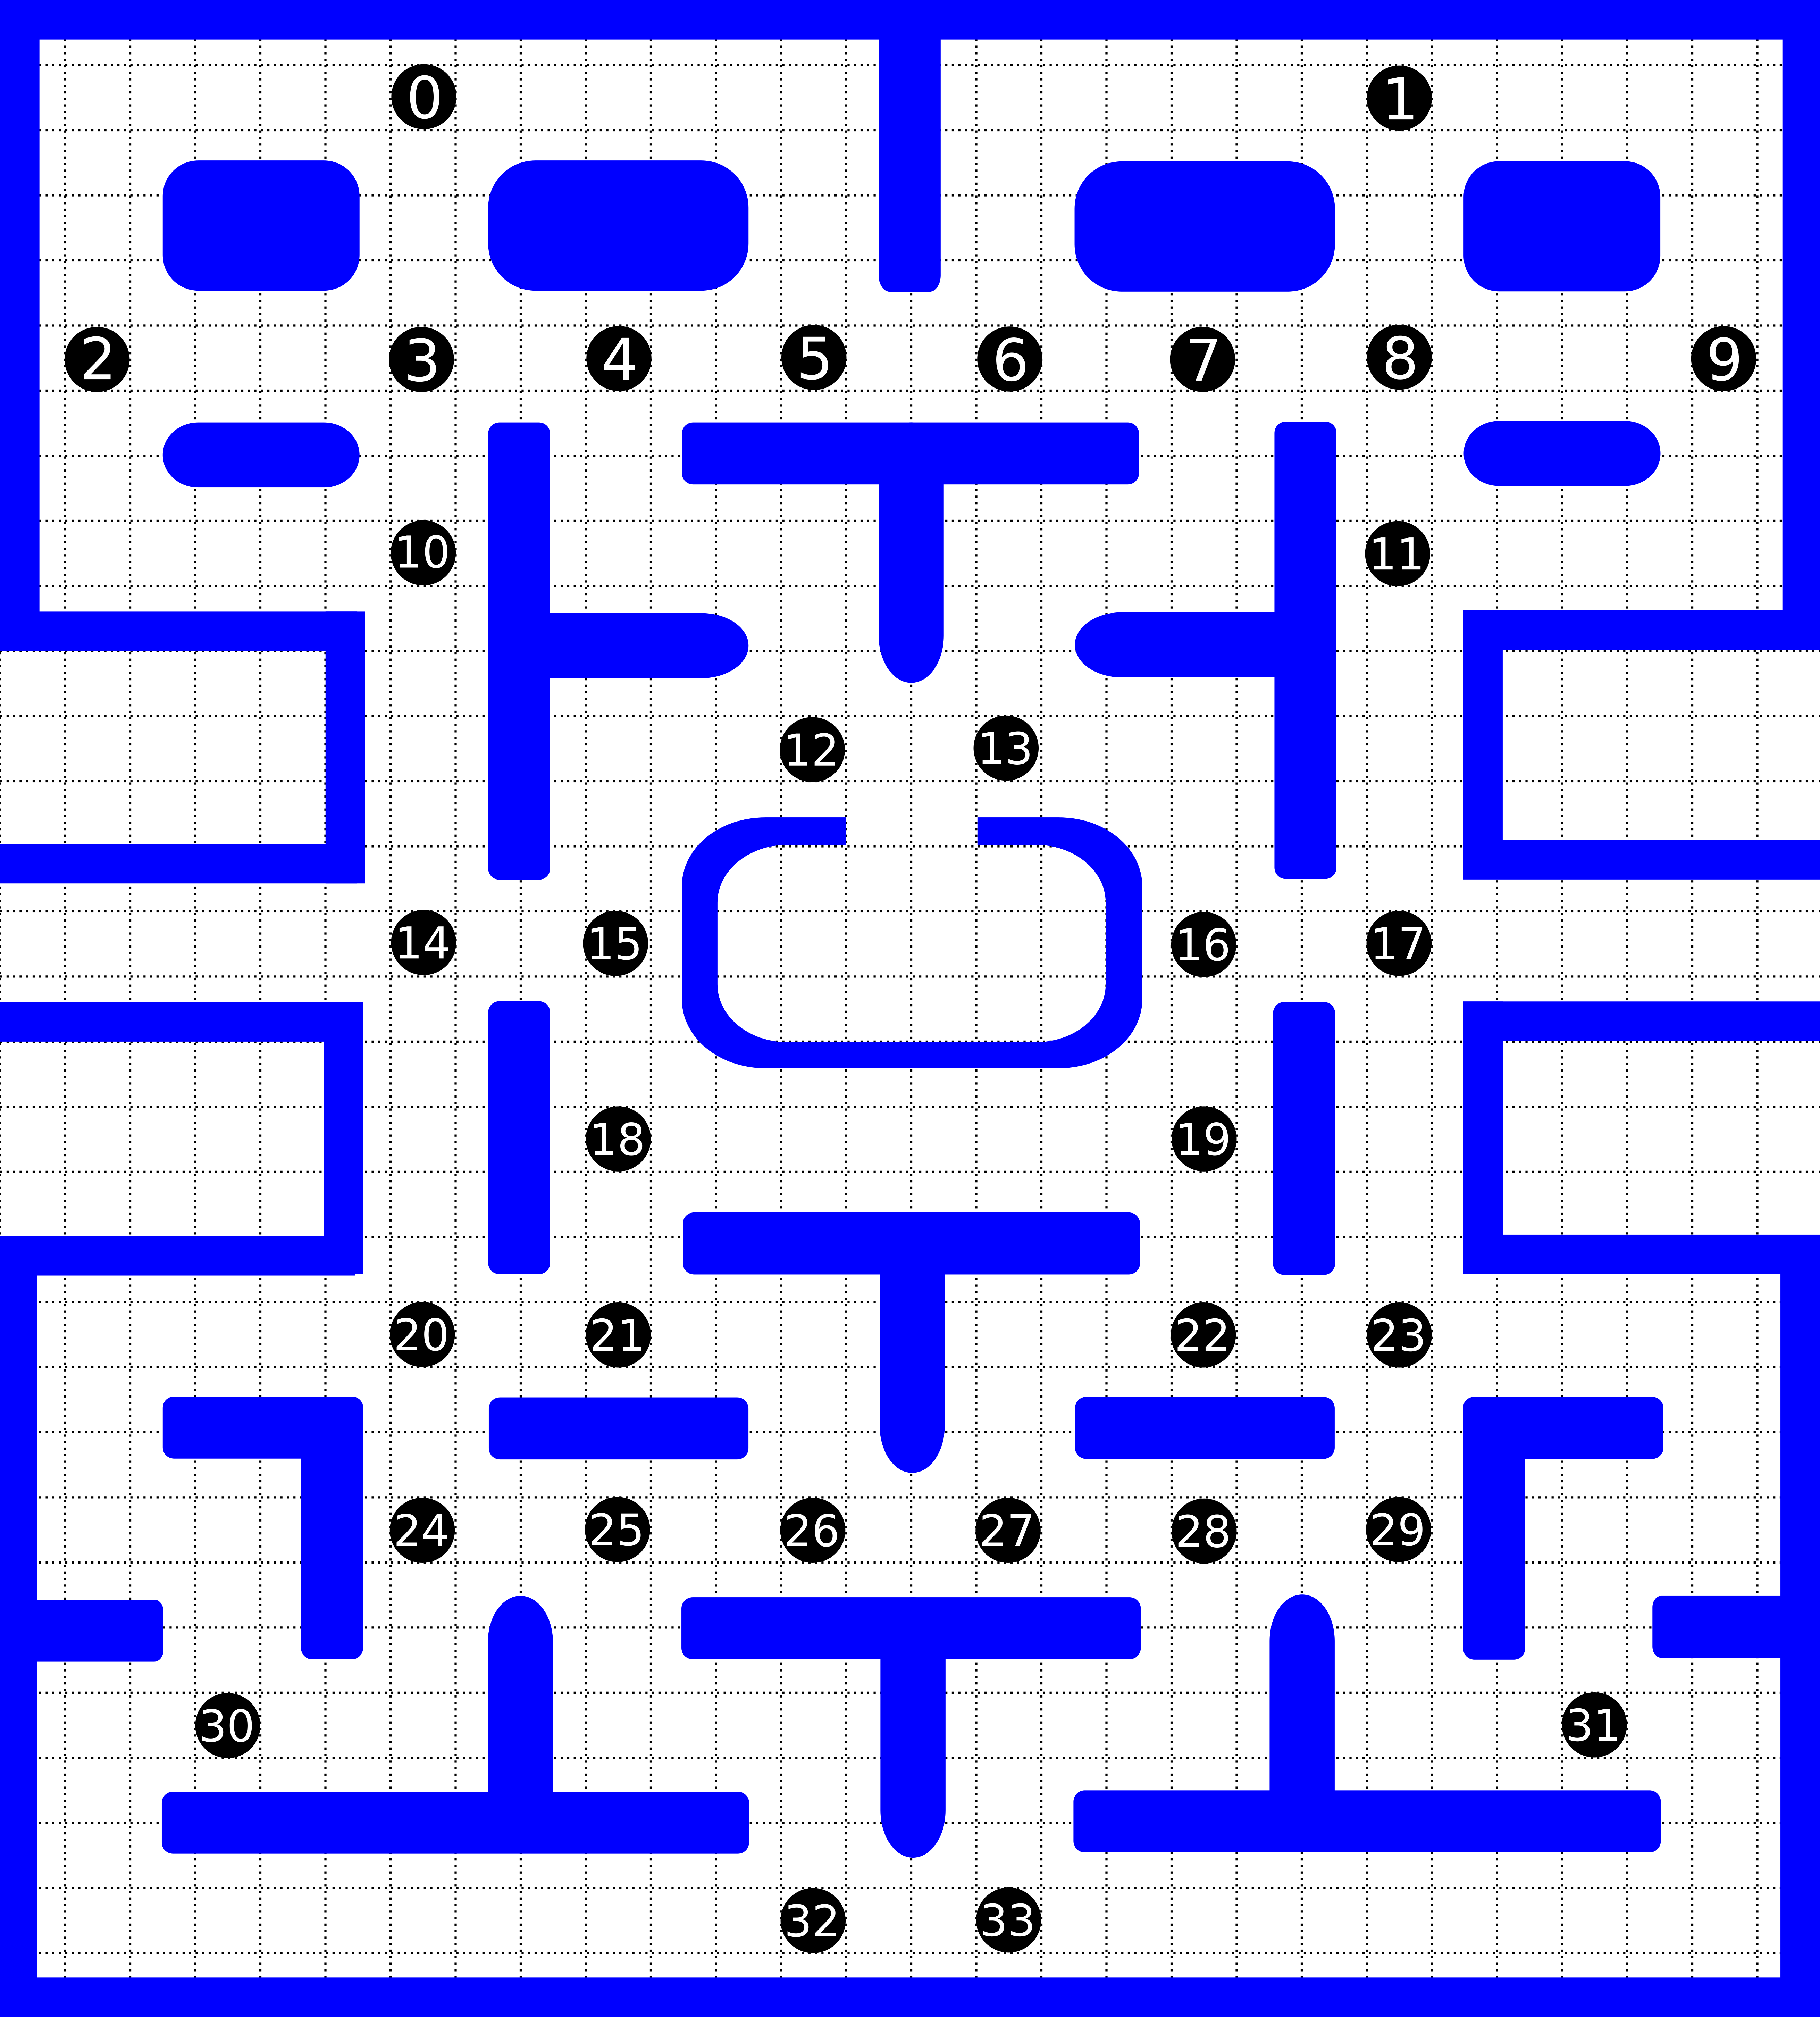
\includegraphics[width=\textwidth]{img/vertici.png}
    \label{lab}
    %\caption{}
   \end{subfigure}
  \begin{subfigure}[b]{0.49\textwidth}
    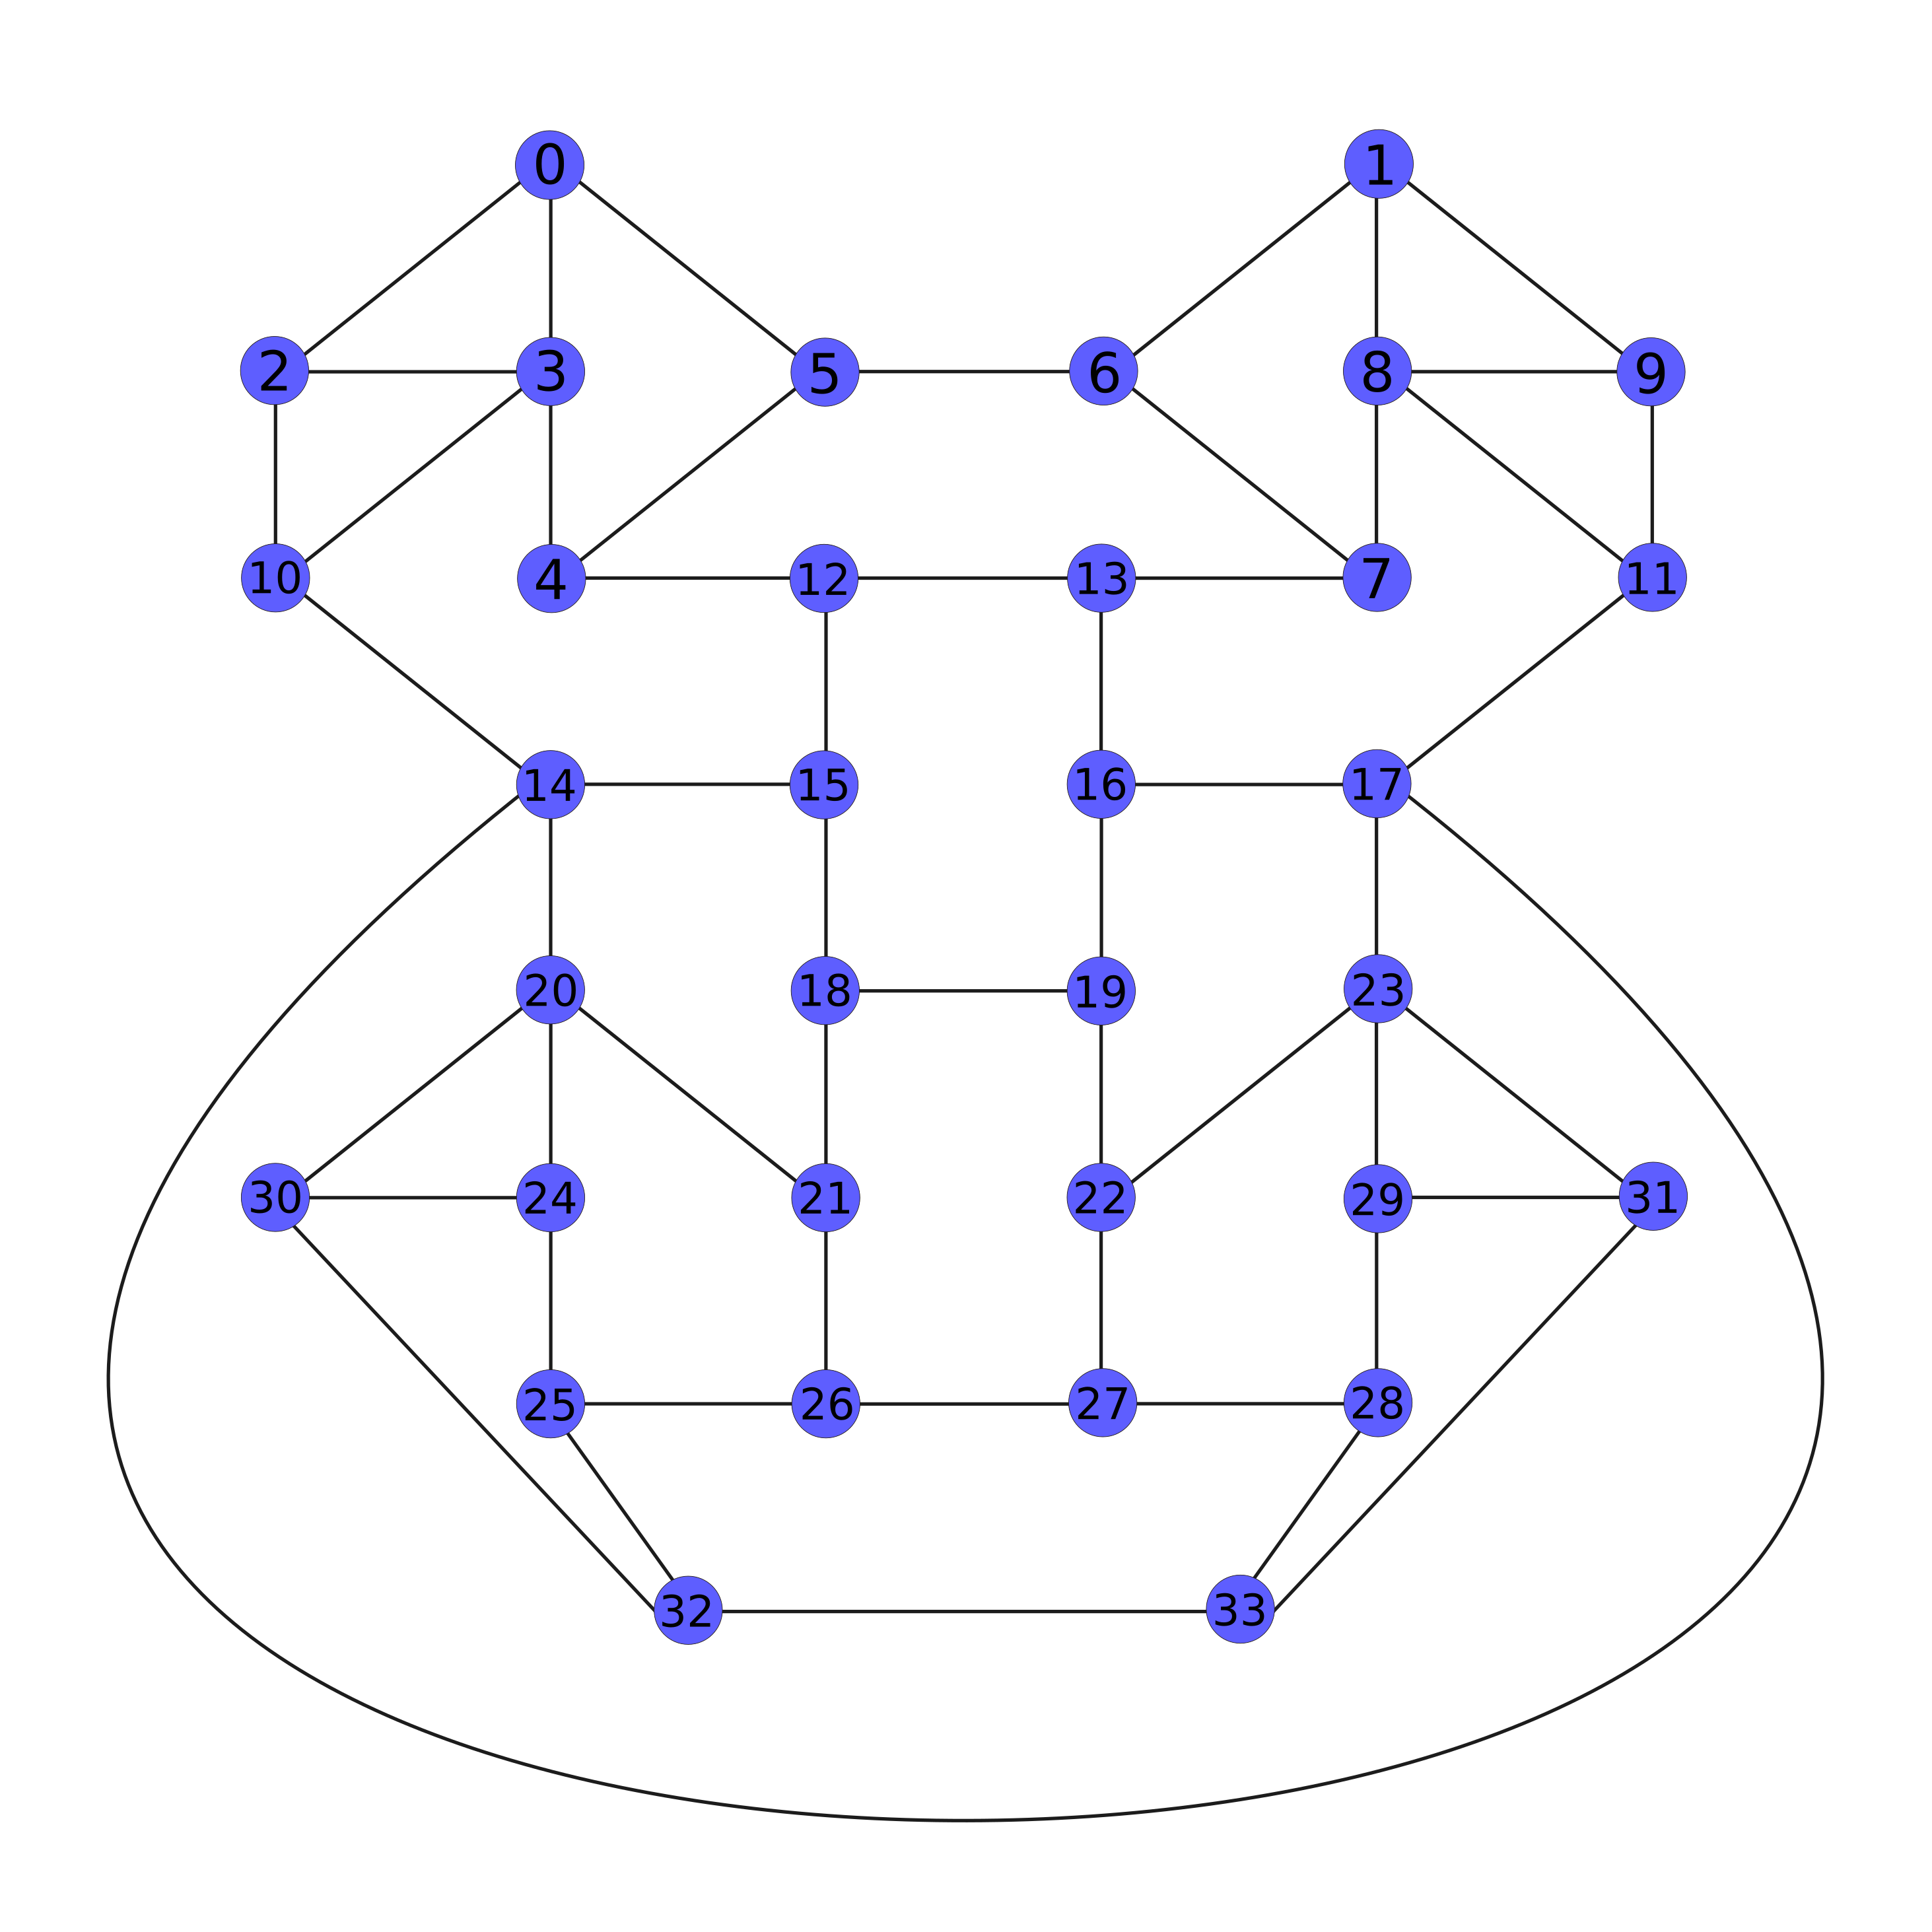
\includegraphics[width=\textwidth]{img/grafoNumeri.png}
    \label{graf}
    %\caption{}
  \end{subfigure}
  \label{grafoELabirinto}
  \caption{L'indice (o etichetta) di ogni incrocio nel labirinto (sinistra).\\Le etichette vengono utilizzate per generare il grafo del labirinto (destra)}
\end{figure}

Il labirinto di Pac-Man viene trasformato in un grafo dichiarando una matrice di vertici e inizializzando ciascuna porta con i vicini del vertice (i campi ianua, che in latino significa porta).

\begin{spacing}{0.9}
  \begin{small}
    \begin{tcolorbox}
\begin{verbatim}
grafo[0].linea = 3;
grafo[0].columna = 6;
grafo[0].index = 0;
grafo[0].ianua[SINISTRA] = 34;
grafo[0].ianua[DESTRA] = 35;
grafo[0].ianua[SU] = -1;
grafo[0].ianua[GIU] = 3;
...
grafo[34].ianua[DESTRA] = 0;
...
grafo[35].ianua[SINISTRA] = 0;
...
grafo[3].ianua[SU] = 0;
\end{verbatim}
  \end{tcolorbox}
    \end{small}
      \end{spacing}
    
    Questo codice fa riferimento al labirinto di figura \ref{grafoNodiAggiunti} in cui sono stati aggiunti alcuni vertici supplementari.

\section[Percorso sub ottimale]{Percorso sub ottimale per coprire il labirinto}\label{tocux5f52}

Il percorso che Pac-Man deve seguire per coprire tutto il labirinto viene deciso ``fuori dal gioco'', cioè a design-time dal programmatore e l'agent ne viene ``informato''.

L'ideale sarebbe quello di percorrere ogni corridoio del labirinto una sola volta, in questo modo si ridurrebbe sicuramente al minimo il tempo di gioco. Nel linguaggio della teoria dei grafi, un percorso che non ripassi mai per uno stesso arco viene detto \emph{percorso euleriano} dal matematico Eulero che per per primo studiò questo problema. La condizione necessaria per poter costruire un percorso euleriano è che il grado (cioè il numero di vicini) di ogni vertice sia un numero pari, condizione non presente nel labirinto del Pac-Man. Dovremo pertanto accontentarci di un percorso sub-ottimale.\\

\textsc{Take home message:} un percorso euleriano richiede un grafo che abbia tutti i vertici di grado pari.

La sequenza di vertici del percorso è memorizzata in un array di numeri interi che rappresentano l'indice di ogni vertice.\\
Questa sequenza di vertici è stata costruita in modo che Pac-Man, percorrendola, passi per tutti i corridoi.\\ 

\begin{spacing}{0.9}
  \begin{small}
    \begin{tcolorbox}
\begin{verbatim}
static int cam[]=
  {
    3,10,38,2,34,0,3,2,3,0,35,5,4,3,4,12,13,
    7,6,5,6,36,1,8,7,8,1,37,9,39,11,39,9,8,11,17,
    16,13,12,15,14,17,23,22,19,16,19,15,
    21,40,20,14,20,40,30,42,32,33,43,31,41,
    23,29,31,29,28,33,28,27,22,27,26,21,26,
    25,32,25,24,20,24,30
  };
\end{verbatim}
  \end{tcolorbox}
    \end{small}
      \end{spacing}

\begin{figure}[H]
  \centering
  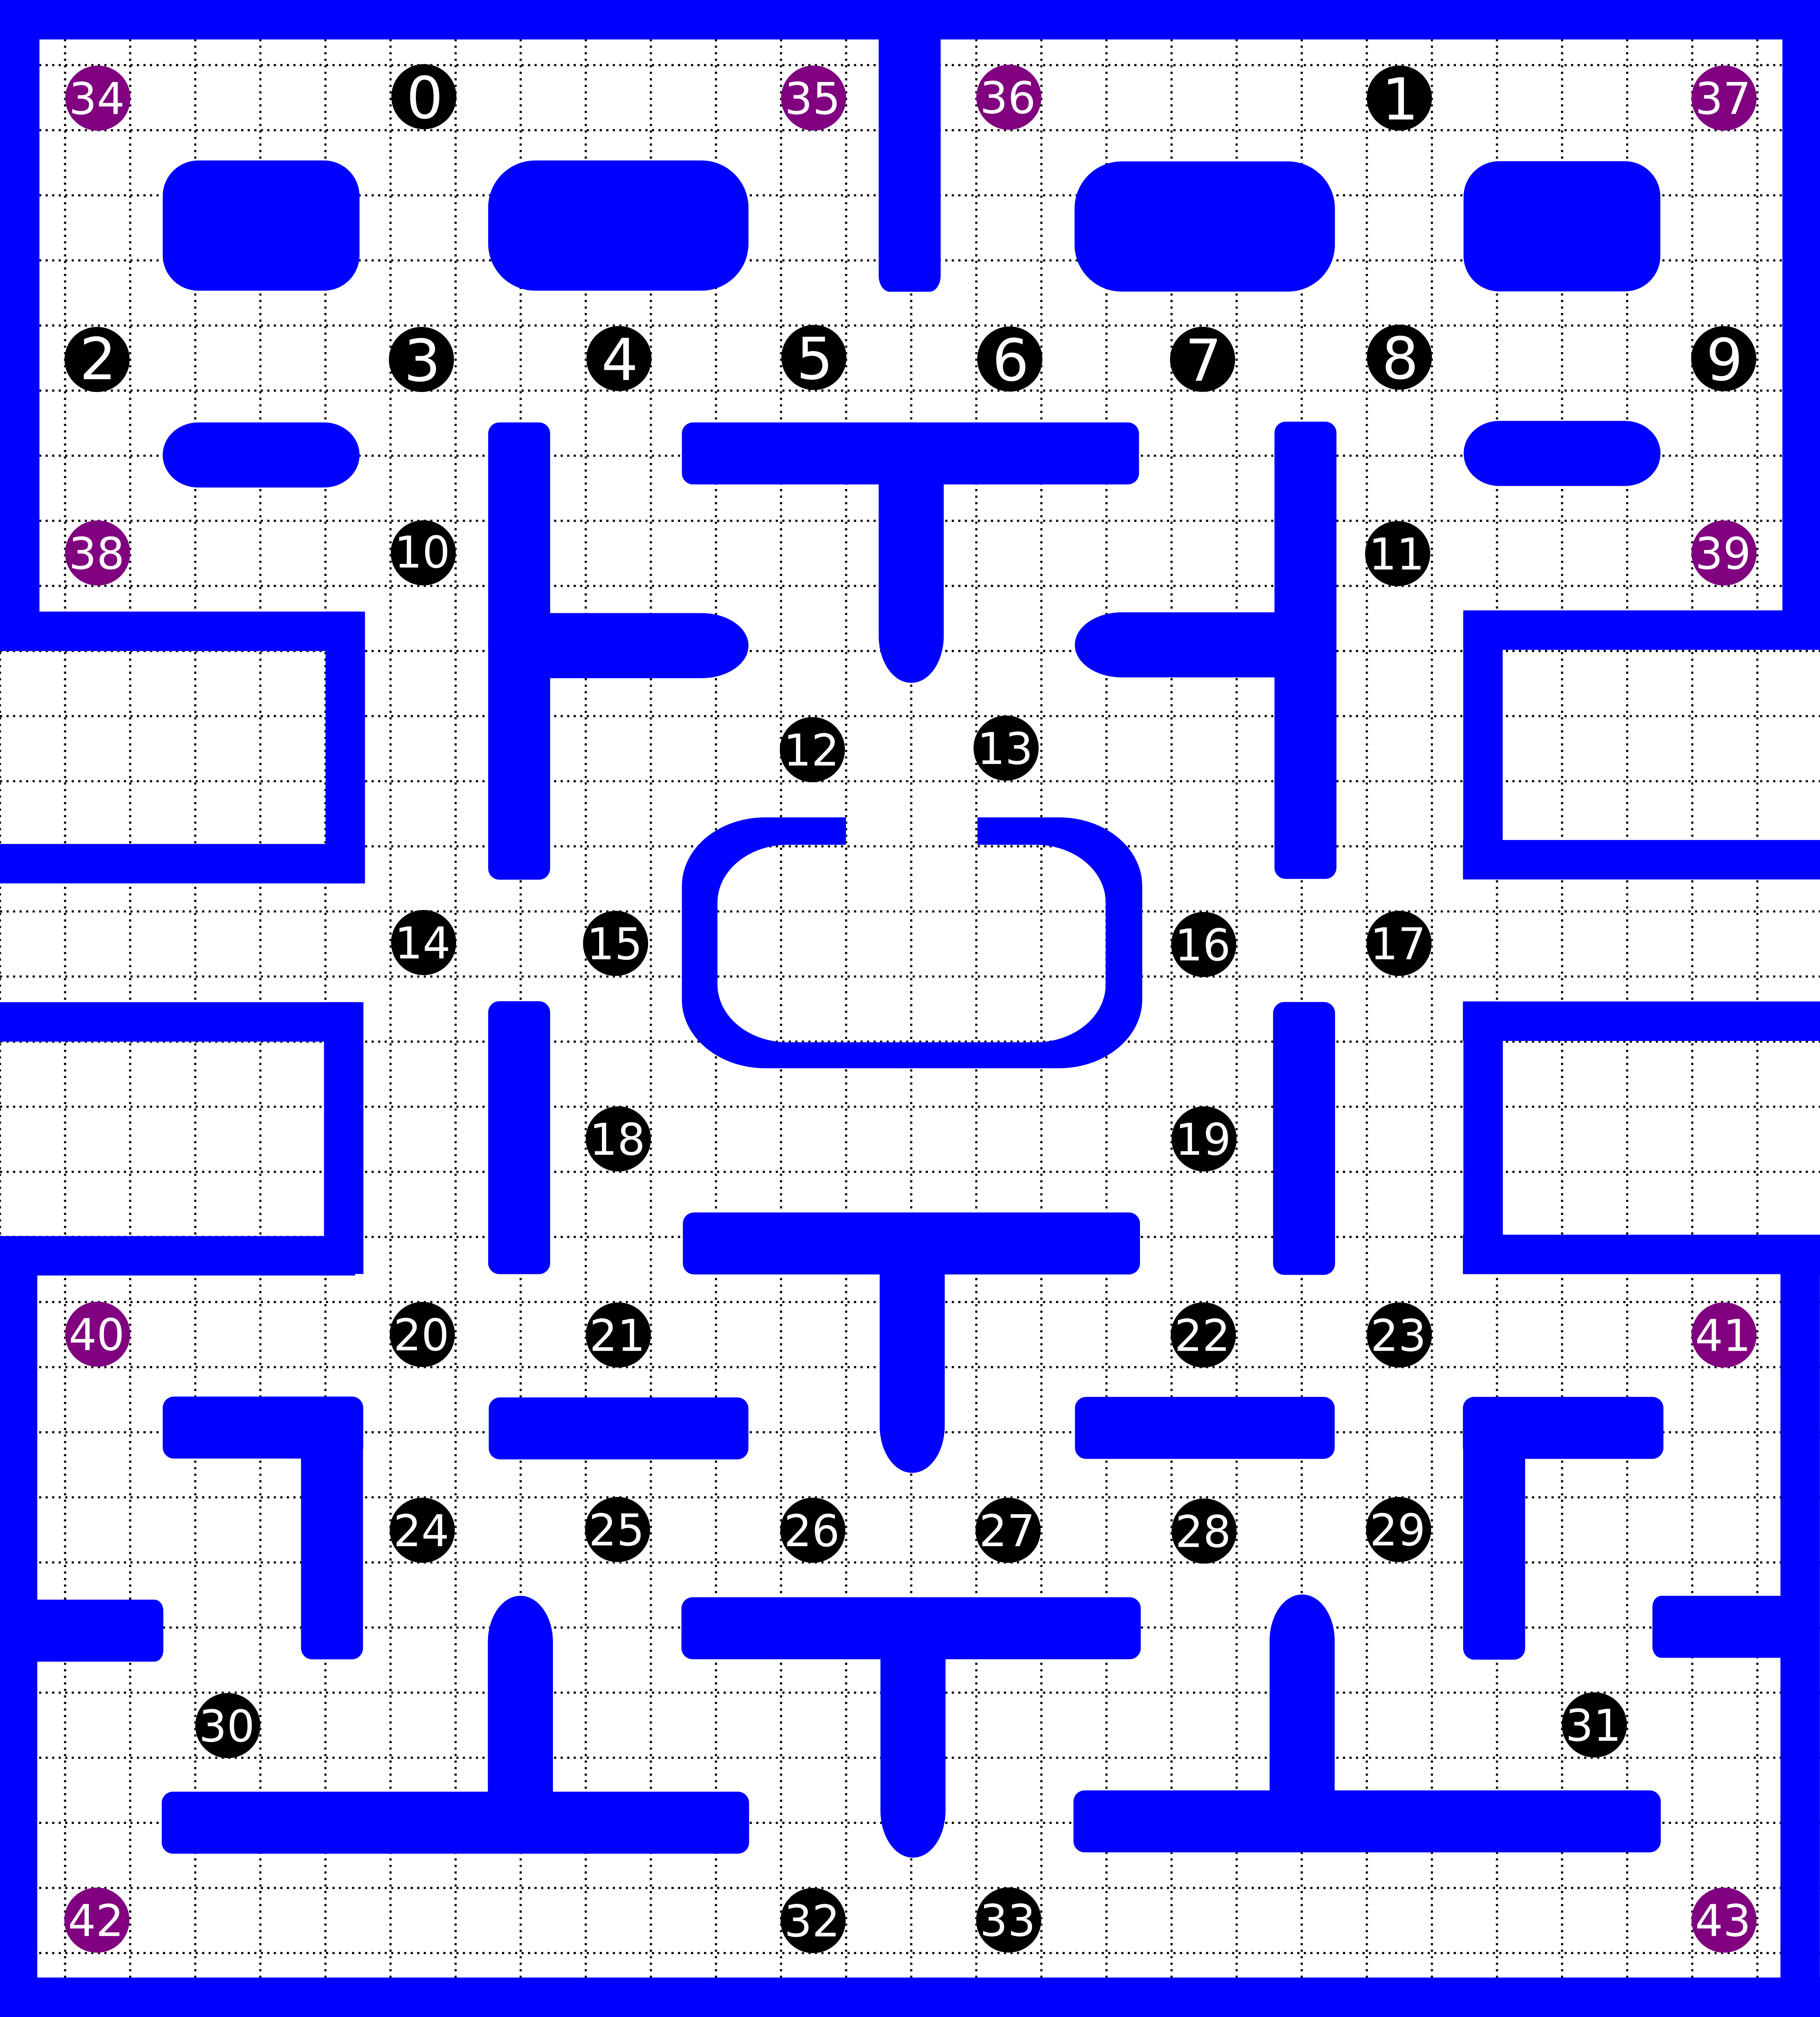
\includegraphics[width=0.5\textwidth]{img/verticiAggiunti.png}
  \caption{I vertici dal 34 al 43 sono stati aggiunti alla rappresentazione originale del grafo}
  \label{grafoNodiAggiunti}
\end{figure}


Ai $34$ vertici di Pac-Man sono stati aggiunti altri dieci, che hanno lo scopo di forzare l'agent ad entrare in alcuni archi che altrimenti avrebbe evitato perché il percorso che li comprende non è il più breve e quindi non è contemplato dall'A*. Ad esempio, l'agent eviterebbe l'angolo in alto a sinistra passando da $2$ a $0$, preferendo passare dal vertice $3$.\\
Quando il gioco inizia il vertice di destinazione è il $3$ (vedi array \texttt{cam}) e il suo percorso dalla posizione iniziale di Pac-Man viene stabilito chiamando l'algoritmo A*.\\
Va notato che è possibile che la posizione iniziale di Pac-Man non sia un vertice, quindi deve vagare nel labirinto fino a raggiungere il primo vertice.

L'agent ha una variabile indice per navigare la matrice \texttt{cam} della sequenza di vertici da seguire per completare il percorso:

\begin{spacing}{0.9}
  \begin{small}
    \begin{tcolorbox}
\begin{verbatim}
int indice_array_vertice_bersaglio = 0;
\end{verbatim}
  \end{tcolorbox}
    \end{small}
      \end{spacing}

Tale indice non viene aggiornato fino a quando non viene raggiunto il vertice di destinazione, a quel punto viene incrementato di un'unità:

\begin{spacing}{0.9}
  \begin{small}
    \begin{tcolorbox}
\begin{verbatim}
if(vertice_corrente == 
   cammino[indice_array_vertice_bersaglio])
  {
    indice_array_vertice_bersaglio++;
    modo_gioco = ESPLORA;
    free(copia);
    copia = 0;
    ...
  }
\end{verbatim}
  \end{tcolorbox}
    \end{small}
      \end{spacing}


\textsc{Take home message:} È possibile utilizzare una sequenza di vertici per specificare un percorso per un agent senza specificare tutte le celle, ad una ad una, per cui l'agent deve passare.\\

Il codice completo \texttt{gioca\_tuki\_percorso.c} si trova in appendice.

\subsection{Compila ed esegui il codice}

Compilare il codice con le seguenti opzioni:

\texttt{
  \newline
  \textasciitilde{}/grafi\textbackslash{}\$ ./compila.sh PacMan/gioca\_tuki\_percorso.c\\ 1 50
  }\\

Quindi esegui specificando nessun fantasma:

\texttt{
  \newline
  \textasciitilde{}/grafi\textbackslash{}\$ ./tuki5.game 0
  }\\

esegui specificando uno o più fantasmi:

\texttt{
  \newline
  \textasciitilde{}/grafi\textbackslash{}\$ ./tuki5.game 1
  }

\newpage
\section*{Box domande n.5}\label{tocux5f109}
\addcontentsline{toc}{section}{Box domande n.5}

\begin{enumerate}
\item Come deve essere un grafo perché sia possibile costruire un \emph{percorso euleriano}?

\begin{enumerate}
\def\labelenumi{\alph{enumi}.}

\item
  Tutti i vertici devono avere un numero pari di vicini
\item
  Tutti i vertici devono essere di grado dispari
\item
  Tutti i vertici devono avere almeno due vicini
\end{enumerate}

\item Dato il seguente labirinto, quale tra questi percorsi permette di coprirlo interamente?

\begin{enumerate}
\def\labelenumi{\alph{enumi}.}

\item
  0-1-6-5-4-0-4-12-4-5-6-7-2-3-9-13\\
  -9-8-7-8-11-10-5-10-14-10-11-15
\item
  0-4-12-4-5-6-1-6-7-2-3-9-13-9-8-11\\
  -15-11-10-14
\item
  15-11-10-14-10-5-4-12-4-0-1-6-7-8-9-3-2
\end{enumerate}

\item Quale tra questi pezzi di codice si riferisce a questo labirinto?

\begin{enumerate}
\def\labelenumi{\alph{enumi}.}

\item
  \texttt{
  grafo{[}5{]}.linea = 4\\
  grafo{[}5{]}.columna = 4\\
  grafo{[}5{]}.index = 5\\
  grafo{[}5{]}.ianua{[}SINISTRA{]} = 4\\
  grafo{[}5{]}.ianua{[}DESTRA{]} = 6\\
  grafo{[}5{]}.ianua{[}SU{]} = -1\\
  grafo{[}5{]}.ianua{[}GIU{]} = 10\\
  }
\item
  \texttt{
  grafo{[}6{]}.linea = 4\\
  grafo{[}6{]}.columna = 7\\
  grafo{[}6{]}.index = 6\\
  grafo{[}6{]}.ianua{[}SINISTRA{]} = 5\\
  grafo{[}6{]}.ianua{[}DESTRA{]} = 7\\
  grafo{[}6{]}.ianua{[}SU{]} = -1\\
  grafo{[}6{]}.ianua{[}GIU{]} = 10\\
  }
\item
  \texttt{
  grafo{[}10{]}.linea = 7\\
  grafo{[}10{]}.columna = 10\\
  grafo{[}10{]}.index = 10\\
  grafo{[}10{]}.ianua{[}SINISTRA{]} = 14\\
  grafo{[}10{]}.ianua{[}DESTRA{]} = 11\\
  grafo{[}10{]}.ianua{[}SU{]} = -1\\
  grafo{[}10{]}.ianua{[}GIU{]} = -1\\
  }
\end{enumerate}

\end{enumerate}


\chapter[Fuga in funzione euristica]{Implementare la fuga nella funzione euristica}

Fin'ora abbiamo ottenuto due risultati importanti. Il primo è che l'agent di Pac-Man riesce a percorrere l'intero labirinto senza il bisogno di essere guidato passo per passo, ma disponendo solo di una lista pre elaborata dei nodi da raggiungere in sequenza. L'agent sfrutta l'algoritmo A* per raggiungerli dalla posizione in cui si trova. Inoltre, quando Pac-man si sposta dalla sequenza di nodi per sfuggire agli attacchi dei fantasmi, l'algoritmo A* gli permette di recuperare rapidamente l'ultima posizione lasciata per fuggire e riprendere la sequenza di nodi programmata in precedenza.

Il secondo risultato è che Pac-Man riesce a completare il labirinto anche in presenza del fantasma Blinky, di cui l'agent è capace di evitare tutti gli attacchi. Questo secondo risultato però non ci deve entusiasmare troppo, infatti dato che ogni vertice ha almeno tre vertici direttamente connessi, cioè nel linguaggio matematico il grafo ha \emph{grado} minimo pari a tre, è normale che l'agent riesca sempre ad evitare Blinky, visto che i due hanno la stessa velocità.

Il meccanismo con il quale l'agent riesce a sfuggire all'attacco di Blinky è basato solo sulla sua capacità di \emph{vedere} il fantasma quando questi si trova ad una certa distanza e quindi di invertire la propria direzione per evitare la \emph{collisione}. In questo paragrafo vediamo invece come sfruttare l'algoritmo A* per evitare Blinky senza bisogno di sfuggirgli direttamente.

\section{Tool di test per A*}

Per meglio comprendere la logica che useremo di seguito conviene scrivere un tool per testare i percorsi calcolati dalla funzione A* senza bisogno di lanciare il gioco. Il codice del tool è piuttosto semplice, si tratta di scrivere una funzione main che accetti come argomento il nodo di partenza e il nodo di destinazione per i quali si vuole calcolare un percorso nel labirinto di Pac-Man. La funzione \texttt{main} deve quindi chiamare la funzione A* passandogli come argomento anche le due funzioni per la stima e il calcolo esatto della distanza. Ovviamente queste due funzioni devono essere definite nel codice del tool e le copiamo esattamente dall'ultima implementazione che abbiamo dato dell'agent. In effetti si tratta di un codice molto semplice, ma per completezza anche questo è riportato in appendice. Si consiglia di editare il codice e di compilarlo. Nel seguito faremo riferimento all'eseguibile chiamandolo \texttt{test\_astar}.

\section{Un ruolo nuovo per l'euristica}

Si è visto che la funzione euristica può essere usata per stimare il percorso più breve tra il nodo di partenza ed il nodo di arrivo.\\
Nell'esempio analizzato abbiamo implementato tale funzione come il calcolo della distanza cartesiana tra le celle relative ai due nodi. È importante capire che la scelta dell'implementazione della funzione euristica è totalmente arbitraria e quindi possiamo implementarla a piacere. È chiaro però che la sua implementazione avrà effetto sul calcolo del percorso ma, come vedremo ora, questo è esattamente quello che vogliamo ottenere.

Usiamo il tool appena scritto (che si trova anche su GitHub) per analizzare il percorso calcolato da A* dal vertice di partenza $26$ al vertice di arrivo $3$, che sono i vertici iniziali del percorso sub-ottimale definito nel paragrafo precedente.

\texttt{
  \newline
\textasciitilde{}/grafi\textbackslash{}\$ ./test\_astar 26 3
}\\

L'output ci fornisce un percorso costituito dalla lista di vertici: $\{21,18,15,14,10,3\}$

\begin{figure}[H]
  \centering
  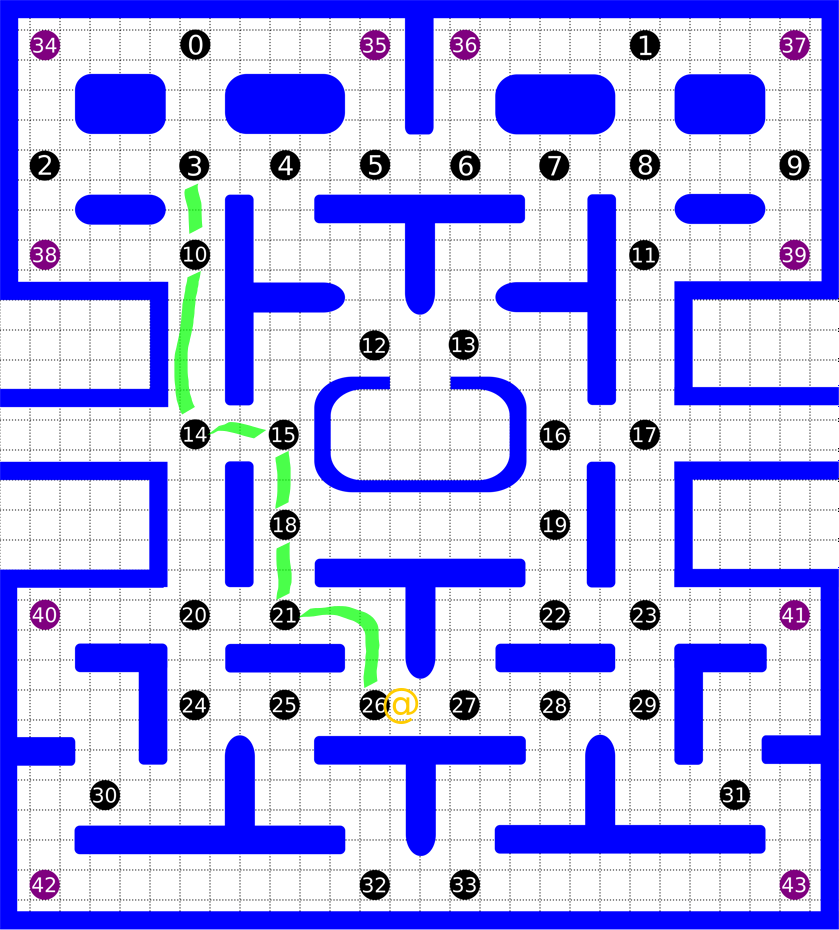
\includegraphics[width=0.5\textwidth]{img/Astar_1.png}
  \caption{Il percorso calcolato da A* tra i vertici $26$ e $3$ è tracciato in verde. Pac-Man è rappresentato con il simbolo @ vicino al vertice $26$.}
  \label{Astar_1}
\end{figure}

Vogliamo provare ad evitare che il percorso di Pac-Man passi per il vertice $15$. Per farlo proveremo a modificare la distanza stimata del vertice $15$ rispetto al $26$, in questo modo l'algoritmo A* preferirà selezionare un percorso che non comprenda il vertice $15$.\\
Modifichiamo la funzione \texttt{euristica\_h} aggiungendo la seguente condizione prima del \texttt{return}:

\begin{spacing}{0.9}
  \begin{small}
    \begin{tcolorbox}
\begin{verbatim}
if(start == 15)
  {
    return 200;
  }
\end{verbatim}
  \end{tcolorbox}
    \end{small}
      \end{spacing}
    
La funzione è quindi definita come segue:

\begin{spacing}{0.9}
  \begin{small}
    \begin{tcolorbox}
\begin{verbatim}
double euristica_h(int start, int goal)
{
  int x1,x2,y1,y2;
  double d;
  x1 = grafo[start].columna;
  y1 = grafo[start].linea;
  x2 = grafo[goal].columna;
  y2 = grafo[goal].linea;
  //Euristica uguale al quadrato della distanza euclidea
  d = (x1-x2)*(x1-x2)+(y1-y2)*(y1-y2);
  if(start == 15)
    {
      return 200;
    }
  return sqrt(d);
}
\end{verbatim}
  \end{tcolorbox}
    \end{small}
      \end{spacing}

Il senso della modifica risulta chiaro se si ricorda che la funzione euristica viene chiamata dalla funzione A* per ogni vertice che deve essere valutato al fine della definizione del percorso. Ad ogni chiamata l'indice del vertice in valutazione è memorizzato nel parametro \texttt{start} mentre nel parametro goal è fisso l'indice $26$ (con riferimento all'esempio che stiamo valutando).\\

La condizione:

\begin{spacing}{0.9}
  \begin{small}
    \begin{tcolorbox}
\begin{verbatim}
if(start == 15)
  {
    return 200;
  }
\end{verbatim}
  \end{tcolorbox}
    \end{small}
      \end{spacing}
    
    fa si che il vertice $15$ risulti molto lontano dal $26$, finendo per essere scartato dal percorso calcolato dall'algoritmo.

Si compili il codice con la modifica apportata e si esegua ancora con la stessa linea di comando:

\texttt{
  \newline
  \textasciitilde{}/grafi\textbackslash{}\$ ./test\_astar 26 3
  }\\

L'output ci fornisce un percorso diverso da prima, costituito dalla lista di vertici: $\{25,24,20,14,10,3\}$

\begin{figure}
  \centering
  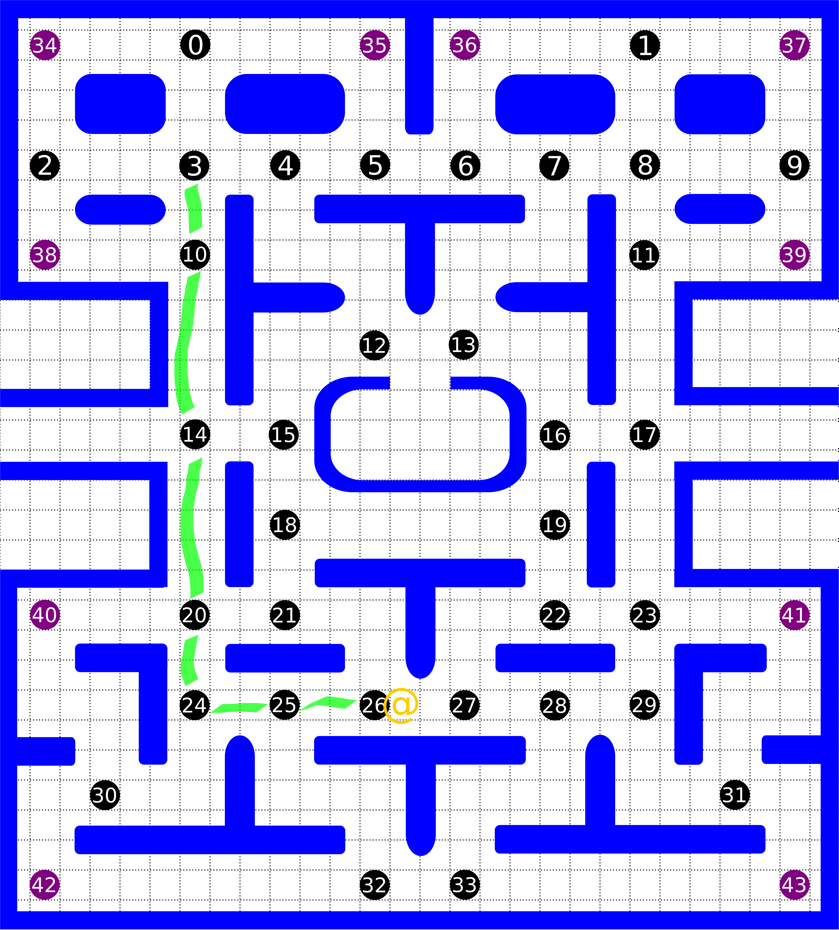
\includegraphics[width=0.5\textwidth]{img/Astar_2.png}
  \caption{Percorso calcolato da A* tra i vertici $26$ e $3$. Pac-Man è rappresentato con il simbolo @ vicino al vertice $26$.}
  \label{Astar_2}
\end{figure}

La funzione euristica, così come la distanza esatta non devono rispettare delle leggi imposte dall'esterno, ma possono essere implementate a piacere per applicare la logica del problema a cui si stanno applicando i grafi.\\
Per esempio i navigatori satellitari, quando calcolano un percorso da seguire con l'automobile, non sono costretti a calcolare per forza il percorso più breve ma possono evitare dei vertici (per esempio strade o incroci) in cui il traffico sia in quel momento troppo intenso.\\
In questo primo semplice esempio abbiamo visto come evitare un vertice in modo hard coded cioè il vertice da evitare è stato memorizzato già nel codice prima di compilarlo e di eseguirlo. Nel prossimo paragrafo vediamo come stabilire un vertice da evitare a \emph{runtime} in base alla configurazione istantanea del gioco.

\section{Test dinamico Pac-Man e Blinky}

Vediamo ora come mettere a frutto l'idea sviluppata nel paragrafo precedente applicandola al contesto di fuga di Pac-Man dal singolo fantasma Blinky.

Per semplificare la trattazione eseguiamo una serie di \emph{esperimenti} usando il tool di test, e riserviamo l'implementazione nell'agent di Pac-Man a quando ci saremo chiariti bene le idee su come procedere.

Faremo anzitutto le seguenti ipotesi semplificative:

\begin{enumerate}
\item
  Pac-Man si muove da vertice a vertice
\item
  Blinky segue un percorso predefinito
\end{enumerate}

che ci permettono di analizzare il problema in modo prototipale sfruttando il tool di test. Rispetto a quanto implementato nel listato \texttt{gioca\_tuki\_percorso.c} mancherà lo stato di \texttt{NAVIGA}, cioè lo stato in cui si trova l'agent mentre si sposta da un vertice all'altro.

Come primo passo modifichiamo la funzione \texttt{main} in modo che percorra iterativamente tutti i vertici calcolati da A* fino al raggiungimento del goal.

\begin{spacing}{0.9}
  \begin{small}
    \begin{tcolorbox}
\begin{verbatim}
/*_______________________________
 * 
 * MAIN 2
 */
int main(int argc, char * argv[])
{
  int s = atoi(argv[1]);
  int g = atoi(argv[2]);
  
  collega_tuki_nodi();
  
  while(s != g)
    {
      printf("%d- \t",s);
      agri_Via pc = 
        agri_astar
        (s,g,grafo,&distanza_esatta,&euristica_h,44);
      s = *pc;
      while(*pc>=0)
        {
          printf("%d\t",*pc);
          pc++;
        }
      printf("\n");
    }
}
\end{verbatim}
  \end{tcolorbox}
    \end{small}
      \end{spacing}

In questo codice il percorso viene continuamente ricalcolato ad ogni vertice raggiunto. Questo comportamento è diverso da quello implementato in precedenza nel codice dell'agent, dove per \emph{risparmiare} CPU, una volta ottenuta la lista dei vertici da percorrere non si richiamava più l'A* a meno che un attacco di Blinky non portasse Pac-Man fuori rotta.\\

Compilando ed eseguendo di nuovo il codice:

\texttt{
  \newline
  \textasciitilde{}/grafi\textbackslash{}\$ ./test\_astar 26 3
  }\\

si ottiene l'output seguente:

\texttt{
  \newline
26-\textgreater{} 21 18 15 14 10 3\\
21-\textgreater{} 18 15 14 10 3\\
18-\textgreater{} 15 14 10 3\\
15-\textgreater{} 14 10 3\\
14-\textgreater{} 10 3\\
10-\textgreater{} 3\\
}

dove ogni riga rappresenta la lista di vertici da percorrere per arrivare al traguardo.

Ora inseriamo nella \texttt{main} una semplice simulazione del movimento di Blinky. In pratica creiamo un array che contiene la sequenza dei vertici del percorso del fantasma e, come già fatto per Pac-Man, supponiamo che anche il rosso antagonista si muova da vertice a vertice senza perdere tempo lungo gli archi.\\
Dichiariamo le variabili globali

\begin{spacing}{0.9}
  \begin{small}
    \begin{tcolorbox}
\begin{verbatim}
int b_iter[]={13,12,15,14,17,14,15,12,13,16,17,14,10};
int passo;
\end{verbatim}
  \end{tcolorbox}
    \end{small}
      \end{spacing}

in testa al listato e modifichiamo la \texttt{main} incrementando la variabile globale passo prima della chiusura del ciclo:\\

\begin{spacing}{0.9}
  \begin{small}
    \begin{tcolorbox}
\begin{verbatim}
while(s != g)
  {
    ...
    printf(":%d\n",b_iter[passo]);
    passo += 1;
  }
\end{verbatim}
  \end{tcolorbox}
    \end{small}
      \end{spacing}


Manca ancora una modifica da fare sulla funzione \\\texttt{euristica\_h}, infatti ora vogliamo che la funzione restituisca una distanza \emph{molto grande} nel caso in cui il vertice \texttt{start} sia un vicino del vertice su cui si trova Blinky. Il codice che implementa questa variazione è il seguente:

\begin{spacing}{0.9}
  \begin{small}
    \begin{tcolorbox}
\begin{verbatim}
if(grafo[b_iter[passo]].ianua[SINISTRA] == start ||
   grafo[b_iter[passo]].ianua[DESTRA] == start ||
   grafo[b_iter[passo]].ianua[SU] == start ||
   grafo[b_iter[passo]].ianua[GIU] == start)
  {
    return 200;
  }
\end{verbatim}
  \end{tcolorbox}
    \end{small}
      \end{spacing}

\subsection{Risultati del test}

Eseguendo:

\texttt{
  \newline
  \textasciitilde{}/grafi\textbackslash{}\$ ./test\_astar 26 3
  }\\

con gli stessi parametri usati prima viene prodotto l'output seguente:

\texttt{
  \newline
26-\textgreater{} 21 18 15 14 10 3 :13\\
21-\textgreater{} 20 14 10 3 :12\\
20-\textgreater{} 24 25 26 27 28 29 23 17 11 8 7 6 5 4 3 :15\\
24-\textgreater{} 25 26 27 22 19 16 13 12 4 3 :14\\
25-\textgreater{} 24 20 14 10 3 :17\\
24-\textgreater{} 25 26 27 22 19 16 13 12 4 3 :14\\
25-\textgreater{} 26 27 28 29 23 17 11 8 7 6 5 4 3 :15\\
26-\textgreater{} 25 24 20 14 10 3 :12\\
25-\textgreater{} 24 20 14 10 3 :13\\
24-\textgreater{} 20 14 10 3 :16\\
20-\textgreater{} 14 10 3 :17\\
14-\textgreater{} 15 12 4 3 :14\\
15-\textgreater{} 14 10 3 :10\\
14-\textgreater{} 10 3 :2\\
10-\textgreater{} 3 :0\\
}

Ogni riga riporta la lista dei vertici su cui muovere Pac-Man a partire dall'ultima posizione occupata, per esempio la prima riga presuppone che il vertice di partenza sia il $26$ e il primo spostamento sia verso il $21$; allo stesso modo la seconda riga assume come vertice di partenza il $21$ e il $20$ come il vertice su cui muovere Pac-Man. Al termine di ogni riga, dopo i due punti, è stampata la posizione di Blinky.

Analizziamo i risultati del test e, per meglio visualizzarli, riportiamo il percorso sul labirinto anche se il test è stato condotto in un grafo più semplice un cui sostanzialmente i vertici sono collegati gli uni agli altri senza i corridoi presenti nel labirinto reale.

\begin{figure}
  \centering
  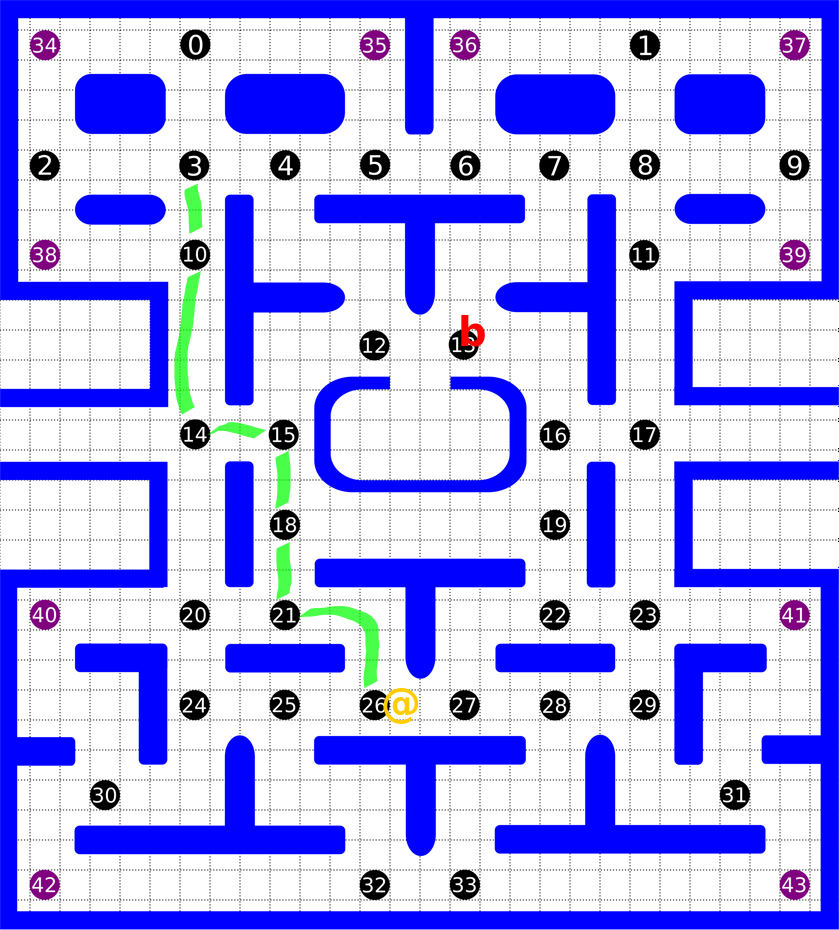
\includegraphics[width=0.5\textwidth]{img/Astar_3_1.png}
  \caption{Percorso calcolato da A* tra i vertici 26 e 3. Pac-Man è rappresentato con il simbolo @ sul vertice 26 mentre Blinky è rappresentato con la lettera b sul vertice 13.}
  \label{Astar_3_1}
\end{figure}


\begin{figure}
  \centering
  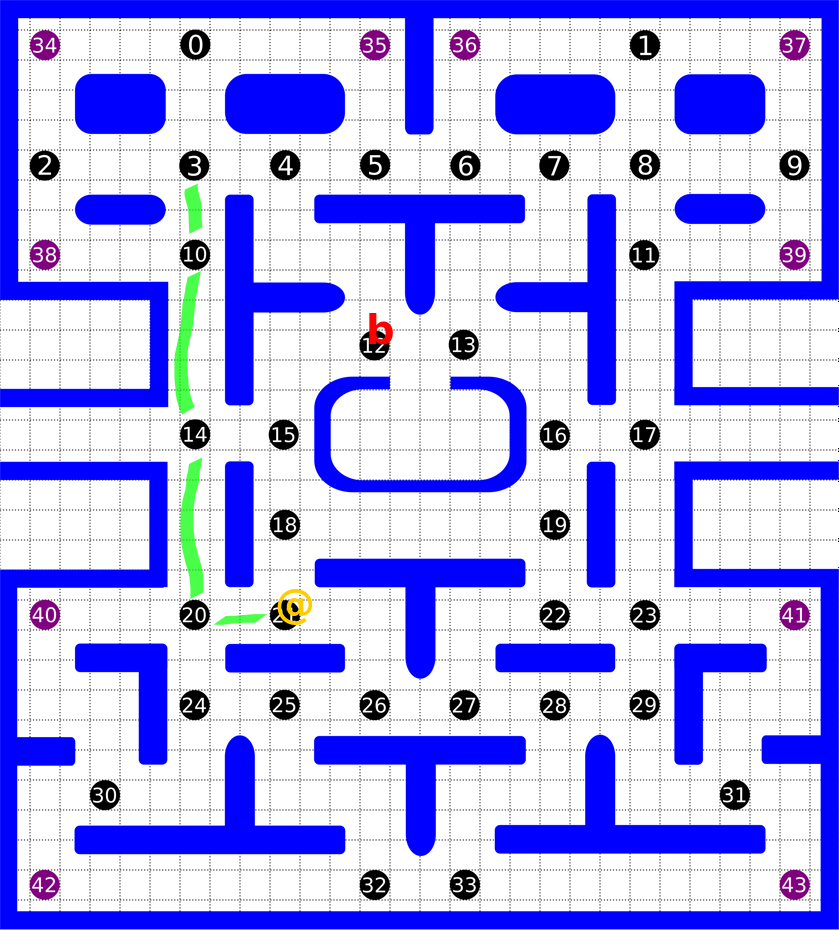
\includegraphics[width=0.5\textwidth]{img/Astar_4_1.png}
  \caption{Percorso calcolato da A* tra i vertici 21 e 3. Il percorso risulta variato rispetto all'iterazione precedente che comprendeva il vertice 14 in quanto ora Blinky può raggiungere tale vertice in un solo movimento.}
  \label{Astar_4_1}
\end{figure}


\begin{figure}
  \centering
  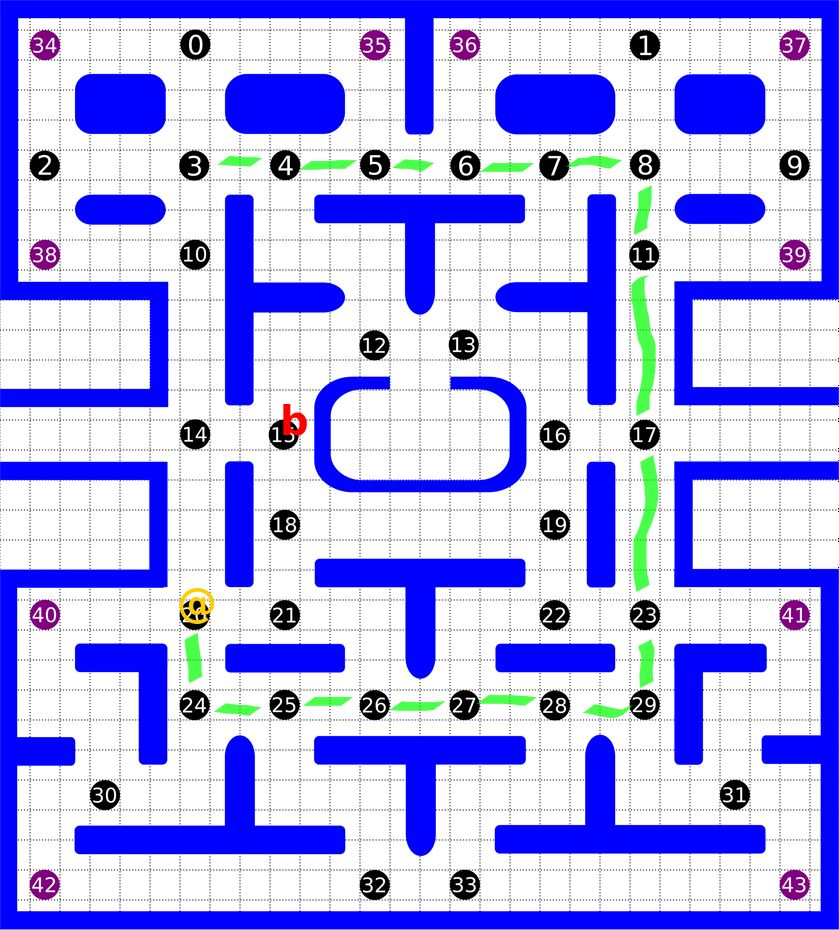
\includegraphics[width=0.5\textwidth]{img/Astar_5.png}
  \caption{Percorso calcolato da A* tra i vertici 20 e 3. Il nuovo percorso risulta il più conveniente come compromesso tra brevità e distanza da Blinky.}
  \label{Astar_5}
\end{figure}
 

Come si è detto, per ogni ciclo, oltre a riportare il cammino pianificato da A*, la \texttt{main} stampa a terminale il vertice su cui si trova Blinky. Inizialmente Blinky è in posizione $13$ e l'A* calcola il percorso come visto in precedenza (figura \ref{Astar_3_1}). Quando però Pac-Man si sposta sul vertice $21$, Blinky si muove sul $12$ che ha come vicino il $15$, quindi la seconda riga risulta modificata rispetto alla prima perché A* ha ricalcolato il percorso per evitare il nodo $15$ (figura \ref{Astar_4_1}). Quando Pac-Man si muove sul nodo $20$, Blinky lo anticipa sul $15$, bloccandogli il cammino verso il $14$ e costringendolo a fare marcia indietro verso il nodo $24$ e ad intraprendere un cammino che circumnaviga la \emph{casa dei fantasmi} che, per quanto risulti lungo, viene comunque valutato più conveniente rispetto a quello che passa per i nodi prossimi a Blinky (figura \ref{Astar_5}).\\
Il resto degli spostamenti può essere dedotto leggendo l'output qui sopra. Il risultato interessante che abbiamo ottenuto è di avere implementato un meccanismo di fuga che non è basato su un controllo diretto della prossimità del fantasma, ma che poggia direttamente su una pianificazione del percorso.

Il risultato che abbiamo ottenuto è molto incoraggiante perché indica una via di \emph{navigazione ragionata} in cui le proprietà dei grafi possono essere usate per evitare anche ostacoli dinamici come appunto la presenza dei fantasmi.\\
Prima di procedere e vedere come riportare questi risultati direttamente dentro la piattaforma di gioco, continuiamo con i test e vediamo se è possibile anche implementare la stessa logica quando i fantasmi sono in numero maggiore di uno.

\section{Test dinamico Pac-Man e Ghost Team}

Iniziamo inserendo nel gioco il fantasma Pinky accanto a Blinky. In questo contesto i nomi ci servono solo a titolo esemplificativo perché i percorsi di attacco che stiamo usando per i fantasmi non rappresentano le loro personalità che sono state spiegate nei capitoli precedenti.

Per simulare la presenza di Pinky aggiungiamo l'array \texttt{p\_iter} alle variabili globali, dichiarandolo subito dopo quello di Blinky.

\begin{spacing}{0.9}
  \begin{small}
    \begin{tcolorbox}
\begin{verbatim}
int p_iter[]={12,13,16,19,22,23,17,11,8,7,6,5,4,3,2,0};
\end{verbatim}
  \end{tcolorbox}
    \end{small}
      \end{spacing}

A questo punto è necessario modificare anche la funzione \texttt{euristica\_h} in modo che tenga conto di entrambi i fantasmi. Per farlo aggiungiamo la condizione seguente subito sotto la precedente condizione già scritta che si riferisce a Blinky:

\begin{spacing}{0.9}
  \begin{small}
    \begin{tcolorbox}
\begin{verbatim}
if(grafo[p_iter[passo]].ianua[SINISTRA] == start ||
   grafo[p_iter[passo]].ianua[DESTRA] == start ||
   grafo[p_iter[passo]].ianua[SU] == start ||
   grafo[p_iter[passo]].ianua[GIU] == start)
  {
    return 200;
  }
\end{verbatim}
  \end{tcolorbox}
    \end{small}
      \end{spacing}

Modifichiamo la main in modo che venga stampata anche la posizione di Pinky oltre a quella di Blinky:

\begin{spacing}{0.9}
  \begin{small}
    \begin{tcolorbox}
\begin{verbatim}
printf(":%d :%d\n",b_iter[passo],p_iter[passo]);
\end{verbatim}
  \end{tcolorbox}
    \end{small}
      \end{spacing}

Eseguiamo di nuovo con lo stesso argomento:

\texttt{
  \newline
  \textasciitilde{}/grafi\textbackslash{}\$ ./test\_astar 26 3
}

\texttt{
  \newline
  26-\textgreater{} 25 24 20 14 10 3 :13 :12\\
  25-\textgreater{} 24 20 14 10 3 :12 :13\\
  24-\textgreater{} 20 14 10 3 :15 :16\\
  20-\textgreater{} 24 25 26 27 28 29 23 17 11 8 7 6 5 4 3 :14 :19\\
  24-\textgreater{} 20 14 10 3 :17 :22\\
  20-\textgreater{} 21 18 19 16 13 12 4 3 :14 :23\\
  21-\textgreater{} 18 15 14 10 3 :15 :17\\
  18-\textgreater{} 21 20 14 10 3 :12 :11\\
  21-\textgreater{} 18 15 14 10 3 :15 :8\\
  18-\textgreater{} 15 12 4 3 :14 :7\\
  15-\textgreater{} 12 4 3 :20 :6\\
  12-\textgreater{} 15 14 10 3 :21 :5\\
  15-\textgreater{} 14 10 3 :18 :4\\
  14-\textgreater{} 10 3 :15 :3\\
  10-\textgreater{} 3 :14 :2\\
}
    

Analizzando le righe dell'output si vede che il calcolo del percorso procede in modo simile all'esempio precedente in cui era coinvolto un singolo fantasma.\\
La situazione però cambia decisamente alla decima riga quando il percorso calcolato dall'A* per Pac-Man si rivela insicuro in quanto passa accanto a Blinky. È naturale chiedersi perché sia stato calcolato un percorso così pericoloso. La risposta però diventa naturale guardando la figura \ref{Astar_6}. Infatti qualsiasi percorso si provi a considerare nel labirinto, per arrivare al vertice $3$ partendo dal $18$ è necessario passare in prossimità o del vertice $14$ su cui è presente Blinky o del vertice $7$ su cui è invece presente Pinky, quindi non esiste, al momento del calcolo, un percorso sicuro. Dal momento che la prossimità a Pinky é valutata nello stesso modo della prossimità a Blinky (cioè una distanza di $200$) l'algoritmo premia il percorso complessivamente più breve, cioè quello che passa accanto a Blinky.


\begin{figure}
  \centering
  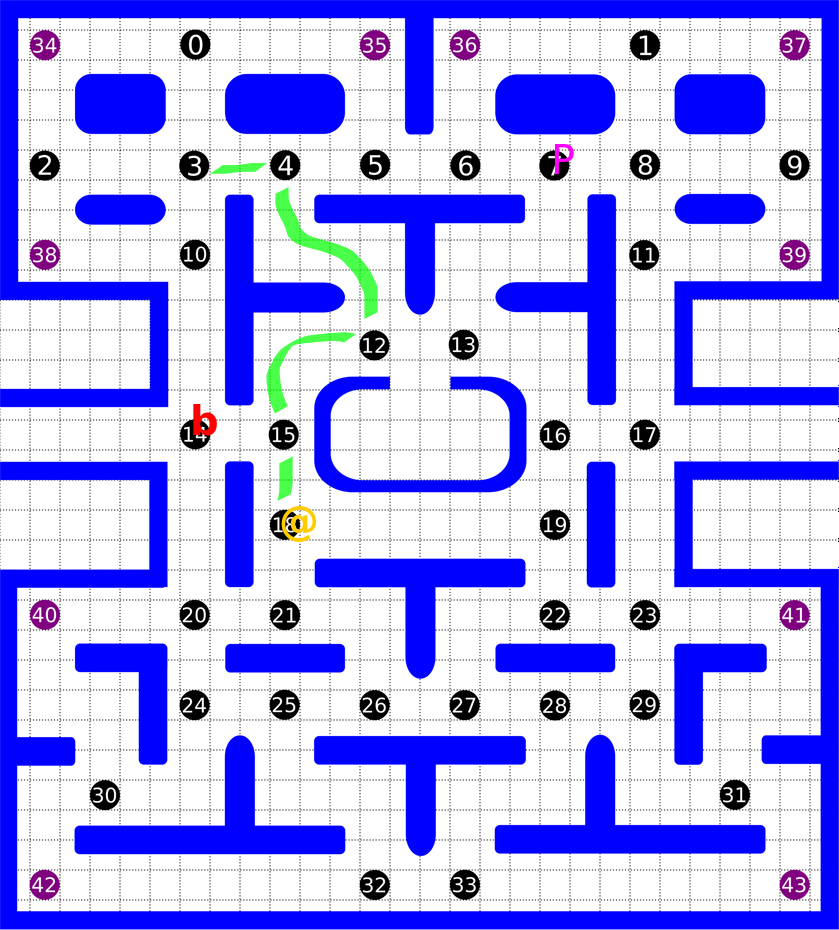
\includegraphics[width=0.5\textwidth]{img/Astar_6.png}
  \caption{Percorso calcolato da A* tra i vertici 18 e 3. Il percorso comprende un vertice contiguo a quello occupato da Blinky.}
  \label{Astar_6}
\end{figure}
 

Il ragionamento appena svolto ci spinge a verificare cosa succede modificando la risposta della \texttt{euristica\_h} in base al fatto che il percorso passi vicino a Blinky o a Pinky. Questa analisi non è fine a sé stessa, infatti come abbiamo visto nei capitoli precedenti ogni fantasma ha una sua personalità e quindi anche una diversa pericolosità, per cui è ragionevole, nell'impossibilità di evitarli del tutto, preferire passare in prossimità di quello meno pericoloso.\\
Per implementare questa nuova caratteristica è sufficiente modificare in

\begin{spacing}{0.9}
  \begin{small}
    \begin{tcolorbox}
\begin{verbatim}
return 225;
\end{verbatim}
  \end{tcolorbox}
    \end{small}
      \end{spacing}

la condizione di controllo sull'array \texttt{p\_iter}.

\begin{spacing}{0.9}
  \begin{small}
    \begin{tcolorbox}
\begin{verbatim}
return 300;
\end{verbatim}
  \end{tcolorbox}
    \end{small}
      \end{spacing}

quella sull'array \texttt{b\_iter}.\\
Ricompiliamo ed eseguiamo e l'output risulta:

\texttt{
  \newline
  26-\textgreater{} 25 24 20 14 10 3 :13 :12\\
  25-\textgreater{} 24 20 14 10 3 :12 :13\\ 
  24-\textgreater{} 25 26 27 22 19 16 17 11 8 7 6 5 4 3 :15 :16\\ 
  25-\textgreater{} 26 27 28 29 23 17 11 8 7 6 5 4 3 :14 :19\\ 
  26-\textgreater{} 21 18 15 14 10 3 :17 :22\\ 
  21-\textgreater{} 18 19 16 13 12 4 3 :14 :23\\
  18-\textgreater{} 19 16 13 7 6 5 4 3 :15 :17\\
  19-\textgreater{} 18 21 20 14 10 3 :12 :11\\
  18-\textgreater{} 19 16 17 11 8 7 6 5 4 3 :15 :8\\
  19-\textgreater{} 16 13 12 4 3 :14 :7\\
  16-\textgreater{} 13 12 4 3 :20 :6\\
  13-\textgreater{} 12 15 14 10 3 :21 :5\\
  12-\textgreater{} 4 3 :18 :4\\
  4-\textgreater{} 3 :15 :3\\
}

\begin{figure}[H]
  \centering
  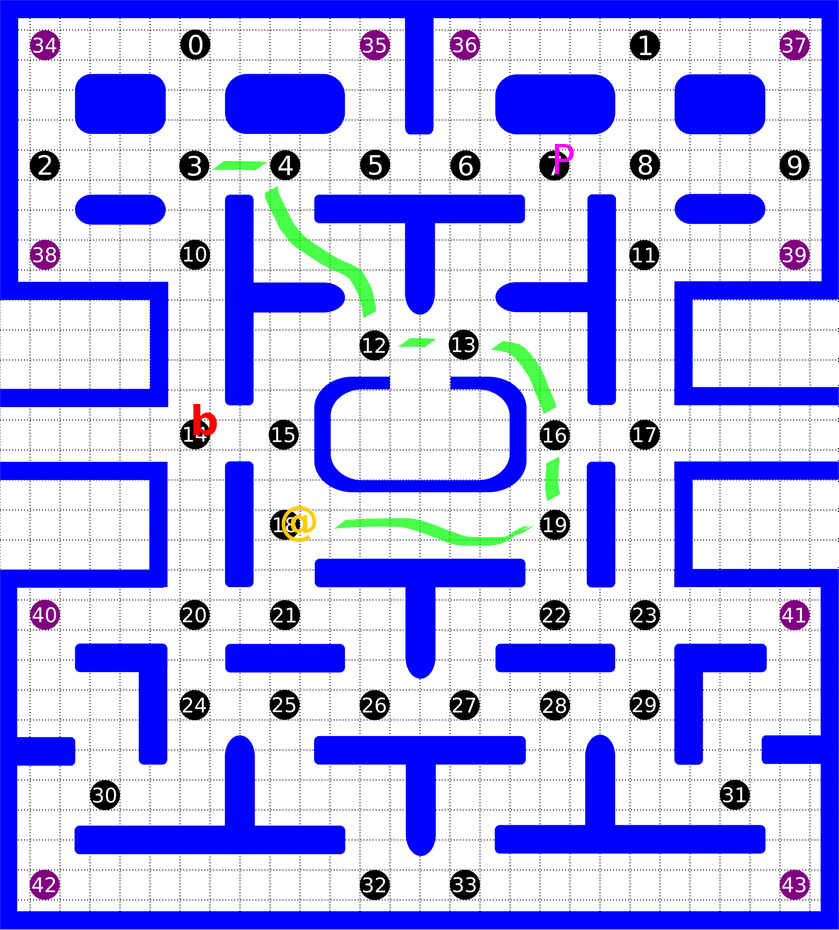
\includegraphics[width=0.5\textwidth]{img/Astar_7.png}
  \caption{Percorso calcolato da A* tra i vertici 18 e 3. Il percorso comprende un vertice contiguo a quello occupato da Pinky.}
  \label{Astar_7}
\end{figure}

Come si vede dai risultati qui sopra, alla riga dieci, questa volta, il percorso calcolato passa vicino a Pinky anziché a Blinky in quanto i nodi vicini a quello di Pinky risultano euristicamente meno lontani dal goal rispetto quelli di Blinky (vedi figura \ref{Astar_7})


\section{Considerazioni}

\begin{wrapfigure}{R}{0.5\textwidth}
  \centering
  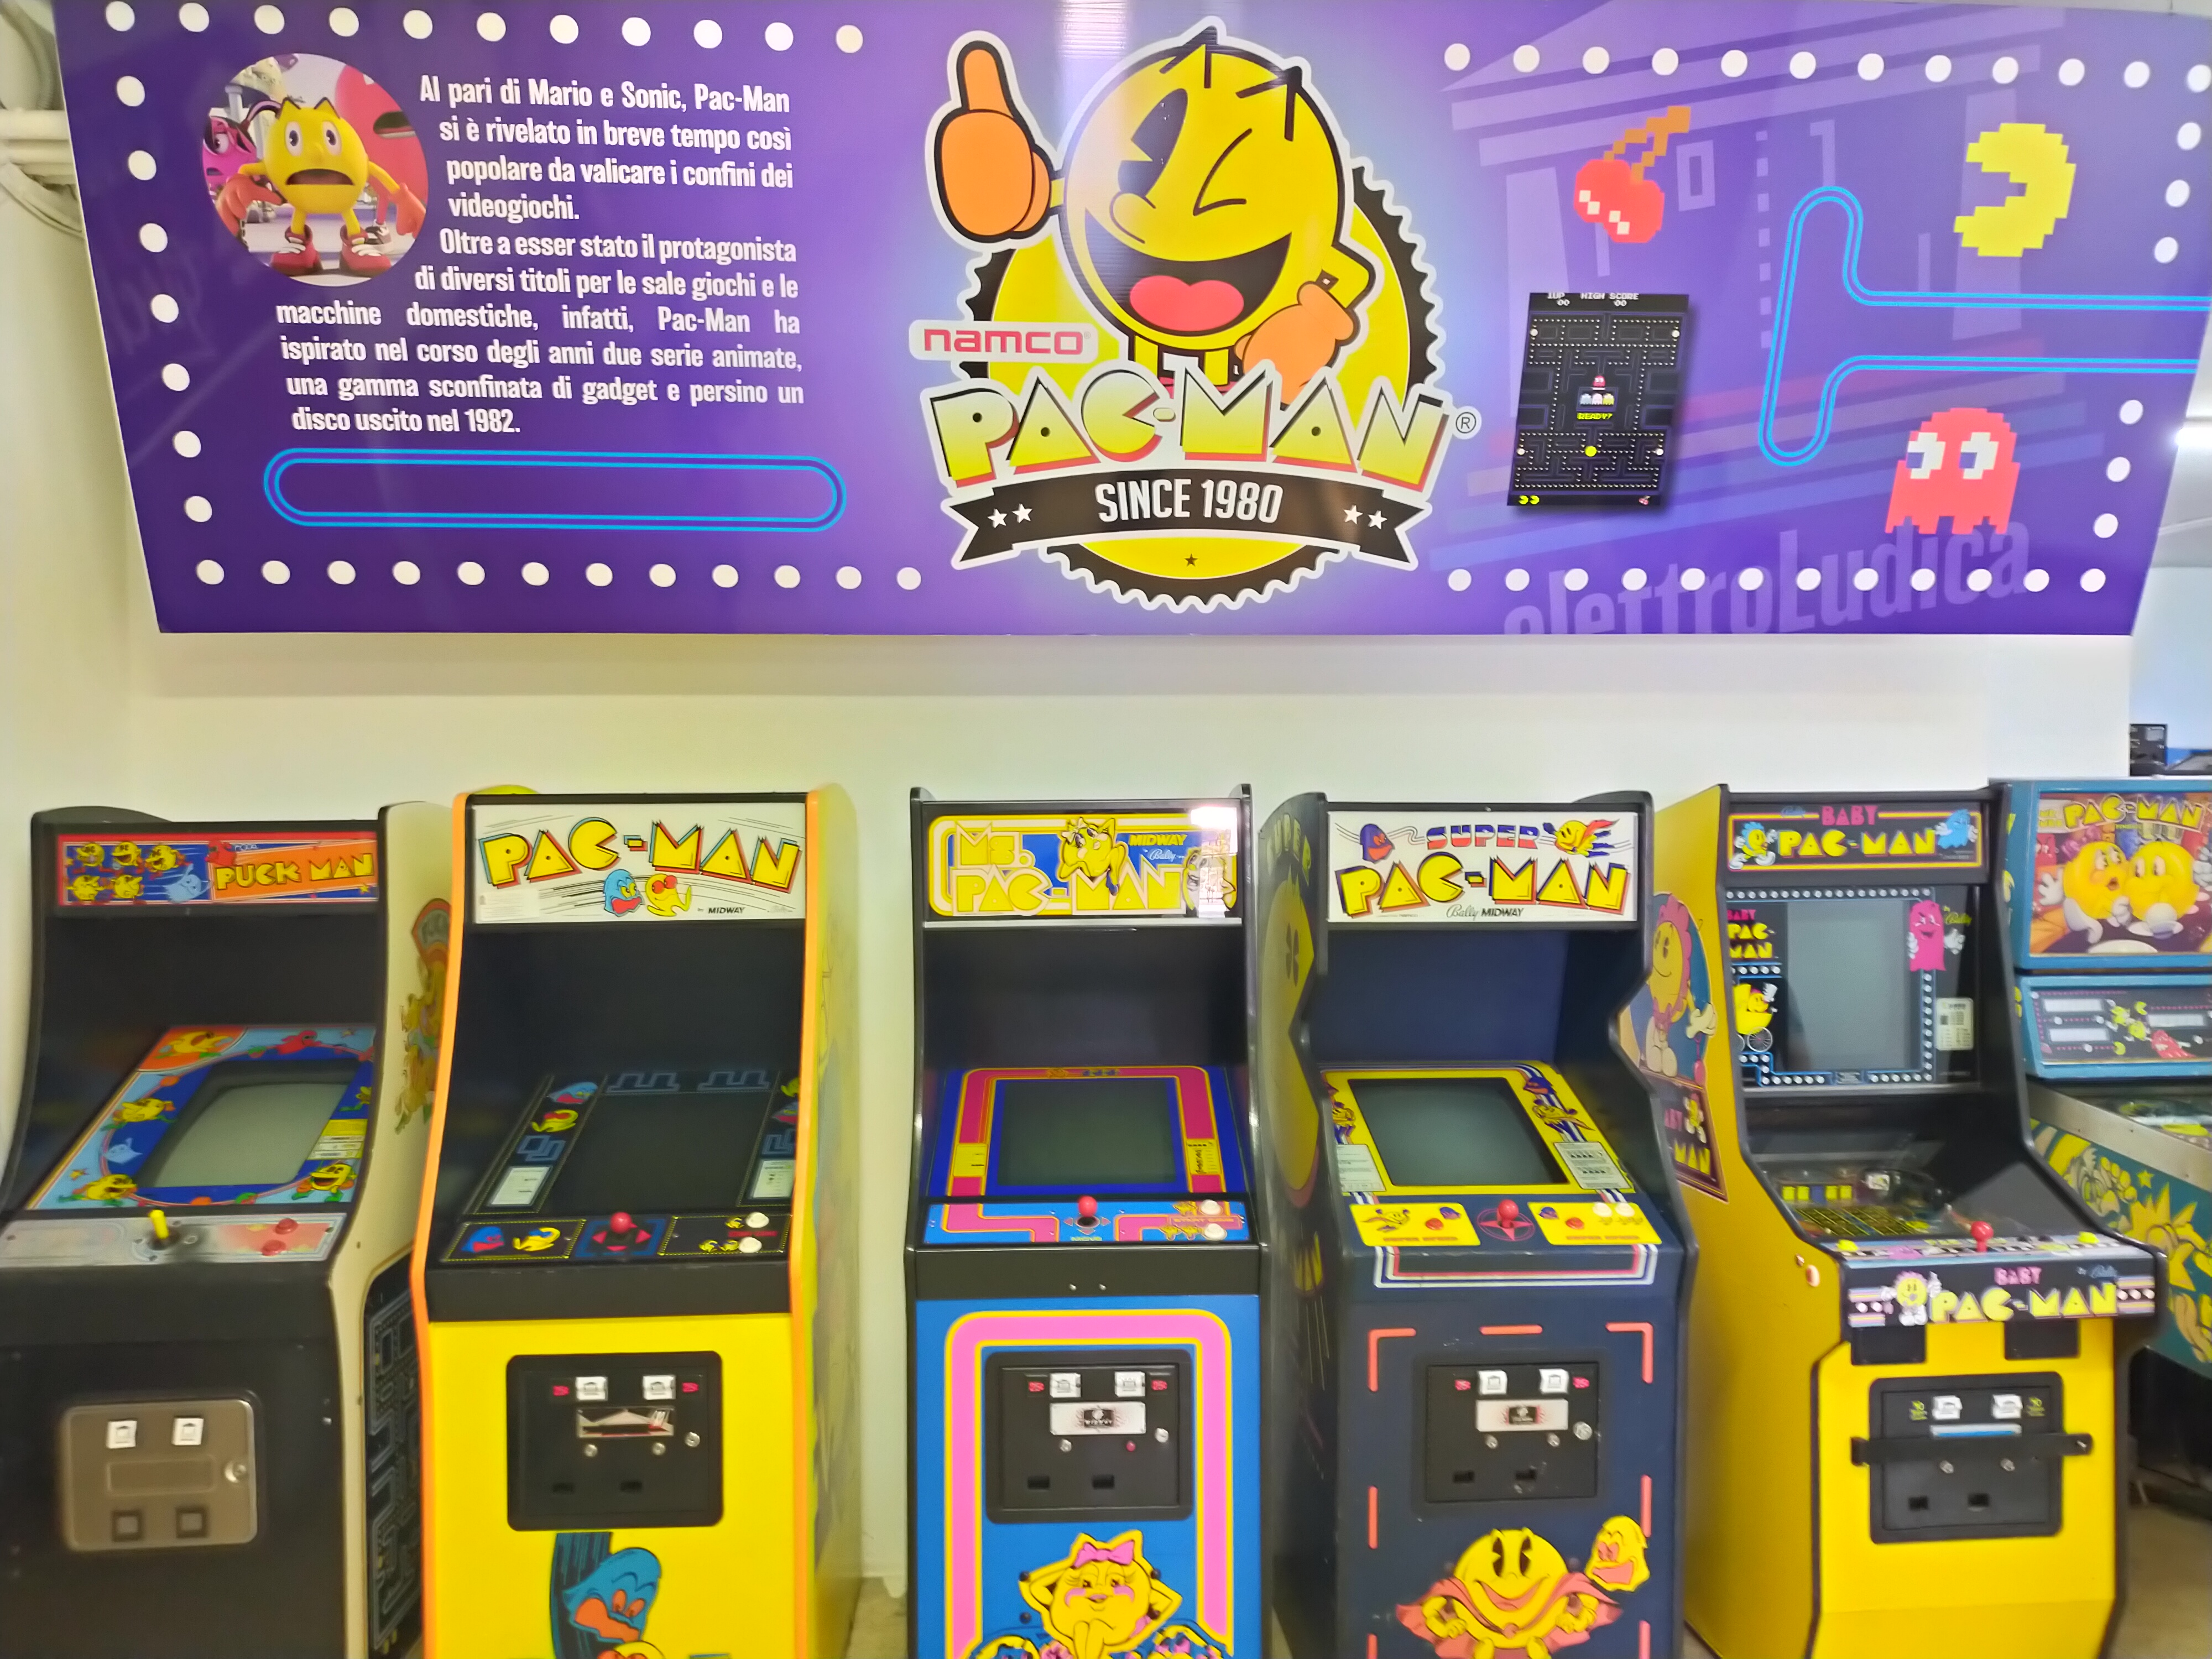
\includegraphics[width=0.5\textwidth]{img/imgConLicenza/postazioni/postazioni.jpg}
  \caption{Museo dell'intrattenimento elettronico, Avezzano, Abruzzo, Italia.}
  \label{postazioni}
\end{wrapfigure}

Prima di proseguire con la ricerca della soluzione alla fuga dell'agent nel labirinto, possiamo trarre alcune considerazioni.\\

La prima è che, data la struttura del labirinto, non esiste una soluzione che possa basarsi puramente sul grafo. Infatti proviamo ad immaginare che i due fantasmi si fissino sulle posizioni $14$ e $7$ appena viste. In questa condizione possiamo anche pensare ad implementare la logica dell'agent in modo da modificare il percorso e preferire i vertici \emph{alti}, cioè quelli che vanno dal $17$ in su (cioè quelli della parte bassa del labirinto), ma quando la sezione inferiore sarà stata completata, il Pac-Man dovrà dedicarsi alla ricerca delle pillole della sezione superiore e finirà obbligatoriamente vittima dell'attacco di un fantasma, anche se fossero solo due.\\

La seconda considerazione è che la preparazione di un percorso da seguire diventa una strategia debole nel momento in cui entrano in gioco i fantasmi e costringono l'agent a fuggire. In quella situazione infatti l'agent fuggendo mangia altre pillole che rendono obsoleti certi passaggi del suo percorso predefinito. Continuando a seguire il percorso l'agent perde tempo e si espone inutilmente al rischio di essere attaccato.\\

Nel prossimo capitolo vediamo come implementare nella piattaforma del gioco le considerazioni svolte.

\chapter{Una pillola\ldots{} vale l'altra}

Nel capitolo precedente abbiamo intuito un possibile modo per trasferire la logica di fuga dell'agent dentro alla funzione che calcola la stima euristica della distanza.\\
Il vantaggio di questo approccio è che Pac-Man non si muove alla cieca verso il suo obiettivo per poi invertire la marcia di fronte alla minaccia dei fantasmi, ma piuttosto pianifica dal principio un percorso che lo tenga lontano dai pericoli.\\

Nel codice di test abbiamo visto che questo approccio può funzionare, ma nel verificarlo abbiamo eseguito alcune semplificazioni che lo hanno astratto dalla piattaforma del gioco. Infatti abbiamo ipotizzato che Pac-Man e i fantasmi si muovessero solo da vertice a vertice senza passare per i corridoi, inoltre abbiamo creato dei percorsi fissi per i fantasmi invece che lasciarli muovere secondo gli algoritmi che ne definiscono le personalità.\\
Vediamo ora come implementare detta logica nel gioco reale.

\section{Grafo completo del labirinto}

Per applicare correttamente la strategia discussa è necessario tener conto che sia Pac-Man che i fantasmi possono trovarsi in una qualsiasi delle celle accessibili e non solo sulle celle che rappresentano un vertice del grafo.\\
Conviene rivedere la logica con cui sono state divise le celle come vertici e archi e ripensare al labirinto come composto solo da celle-vertice connesse tra loro da \emph{archi virtuali}, cioè archi che vengono percorsi istantaneamente e lungo i quali non è possibile stazionare. In pratica ogni cella \emph{accessibile} diventa un vertice che è collegato a tutte le celle \emph{vicine} che come lei risultano accessibili.

Per rappresentare il grafo possiamo continuare ad utilizzare la struttura \texttt{agri\_Vertex} e definire riga e colonna di ogni cella accessibile a Pac-Man. Diversamente da prima non lo faremo direttamente analizzando il grafo, ma modificheremo la funzione \texttt{collega\_tuki\_nodi} perché assegni riga e colonna ad ogni vertice in automatico:

\begin{spacing}{0.9}
  \begin{small}
    \begin{tcolorbox}
\begin{verbatim}
int k = 0;
for(int i = 3; i<ALTEZZA-3; i++)
  {
    for(int j = 1; j<LARGHEZZA-1; j++)
      {
        if( oggetto_accessibile(labx[i][j]))
          {
            grafo[k].linea = i;
            grafo[k].columna = j;
            grafo[k].index = k;
            k++;
          }
      } 
  }
\end{verbatim}
  \end{tcolorbox}
    \end{small}
      \end{spacing}

Con il codice qui sopra abbiamo definito tutti i vertici del grafo, ma questi risultano ancora scollegati gli uni dagli altri. Per collegarli tra di loro è necessario iterare su ognuno di essi e verificare a quali delle celle vicine risulta contiguo.

\begin{spacing}{0.9}
  \begin{small}
    \begin{tcolorbox}
\begin{verbatim}
for(int k = 0; k<NODI_LAB_POT; k++)
  {
    int r = grafo[k].linea;
    int c = grafo[k].columna;
    if(c>0)
      grafo[k].ianua[SINISTRA] =  trova_vertice(r, c-1);
    if(c<LARGHEZZA - 1)
      grafo[k].ianua[DESTRA] = trova_vertice(r, c+1);
    if(r>0)
      grafo[k].ianua[SU] = trova_vertice(r-1, c);
    if(r<ALTEZZA-1)
      grafo[k].ianua[GIU] = trova_vertice(r+1, c);
  } 
\end{verbatim}
  \end{tcolorbox}
    \end{small}
      \end{spacing}

dove la funzione \texttt{trova\_vertice} è analoga alla funzione \\\texttt{indice\_tuki\_nodo\_cella} usata nei codici precedenti.

\section{Implementazione dell'agent}\label{tocux5f88}

Strano ma vero il codice di questo agent è sorprendentemente semplice rispetto quello degli agent visti fin'ora. Infatti la sua logica non prevede alcun meccanismo di fuga, ma solo la scelta \emph{casuale} di un vertice da raggiungere, cioè quello che chiamiamo \emph{goal} e la chiamata continua all'algoritmo A* per conoscere il vertice su cui muoversi.

Sebbene il vertice goal sia scelto casualmente, prima di calcolare il percorso l'agent verifica che in corrispondenza al vertice scelto ci sia una pillola e, in caso contrario, sceglie un altro vertice.\\
Questa modalità di scelta verrà ridiscussa e migliorata nel prossimo capitolo quando vedremo l'uso dell'algoritmo \emph{breadth-first search} per migliorare la navigazione dell'agent all'interno del labirinto.

Come nell'esempio svolto con il codice di test, infatti, non è sufficiente eseguire una singola chiamata ad A* per poi \emph{consumare} uno alla volta i vertici del cammino prodotto, perché ad ogni ciclo di gioco i fantasmi possono spostarsi andando in questo modo a modificare quello che sarebbe il cammino ottimale per raggiungere il \emph{goal}. Per questo motivo, pur mantenendo fisso il goal, il cammino viene ricalcolato ad ogni turno chiamando la funzione \texttt{agri\_astar} e passando come argomento il vertice occupato da Pac-Man e il vertice goal.

\subsection{Risultati}

I risultati di questa implementazione sono piuttosto soddisfacenti, specie se tenuto conto che non è stato implementato nessun algoritmo esplicito per la fuga dai fantasmi.

Per illustrare e discutere le performance di questo agent abbiamo eseguito duecento partite sfidando rispettivamente $1$, $2$, $3$ e $4$ fantasmi per un totale di ottocento partite. Per ogni partita è stato registrato il punteggio totale raggiunto, ricordando che il punteggio di $244$ corrisponde al completamento del labirinto. I risultati ottenuti per l'agent \texttt{gioca\_tuki\_pesato} sono stati confrontati con l'agent \texttt{gioca\_tuki\_percorso} ottenuti con le stesse modalità.

\subsubsection{Blinky}

Lanciando il gioco (\texttt{gioca\_tuki\_pesato}) con il solo fantasma Blinky, l'agent conduce Pac-Man a concludere quasi sistematicamente con successo la partita. Rispetto agli esempi che implementano l'algoritmo di fuga esplicito, vediamo le seguenti differenze:

\begin{itemize}
\item
  Pac-Man non si dirige più spontaneamente verso Blinky per poi cambiare direzione in sua prossimità.
\item
  I percorsi di fuga di Pac-Man non sembrano più \emph{distrarlo} dai suoi vertici obiettivo.
\item
  Pac-Man e Blinky sono mediamente più lontani durante il gioco.
\item
  Pac-Man completa il labirinto in circa metà turni di gioco rispetto a \texttt{gioca\_tuki\_percorso}.
\end{itemize}

In figura \ref{pesatoPercorso1} sono riportati gli istogrammi dei risultati delle partite eseguite usando i due diversi agents. Si nota che mentre l'agent \emph{percorso} ha completato con successo tutte le partite, l'agent \emph{pesato} ha una piccola frazione (circa l'8\%) di partite non completate con successo.

\begin{figure}
  \centering
  \begin{subfigure}[b]{0.49\textwidth}
    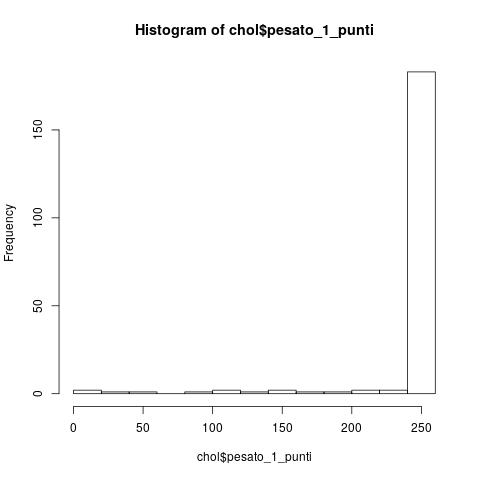
\includegraphics[width=\textwidth]{img/pesato_1_punteggio.png}
    \caption{Pesato1}
    \label{Pesato1}
   \end{subfigure}
  \begin{subfigure}[b]{0.49\textwidth}
    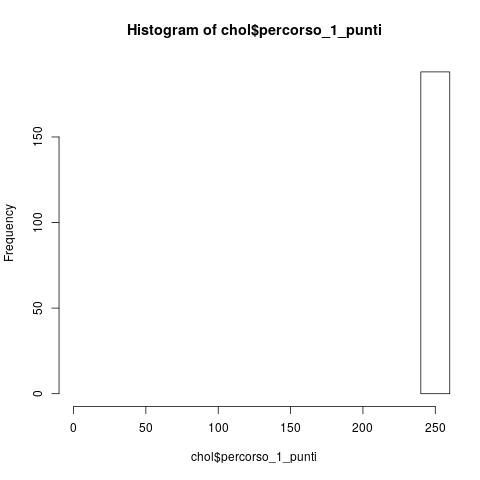
\includegraphics[width=\textwidth]{img/percorso_1_punteggio.png}
    \caption{Percorso1}
    \label{Percorso1}
  \end{subfigure}
  \caption{Istogramma del punteggio raggiunto giocando contro un singolo fantasma. La figura \ref{Pesato1} si riferisce all'agent \emph{pesato}, la \ref{Percorso1} al \emph{percorso}}
  \label{pesatoPercorso1}
\end{figure}


\subsubsection{Blinky e Pinky}

In presenza della coppia Blinky e Pinky le difficoltà di Pac-Man aumentano, ma qui è dove il nuovo agent si distingue decisamente rispetto al primo.\\
Le probabilità di successo dell'agent \emph{pesato} sono vicine al 50\% e comunque il completamento del labirinto risulta essere l'evento relativamente più probabile rispetto a tutti gli altri punteggi (vedi fig. 22).\\
Le cose stanno diversamente per l'agent \emph{percorso} che come si vede da figura 22, da come risultato più probabile la cattura di Pac-Man prima che abbia mangiato venti pillole.

\begin{figure}
  \centering
  \begin{subfigure}[b]{0.49\textwidth}
    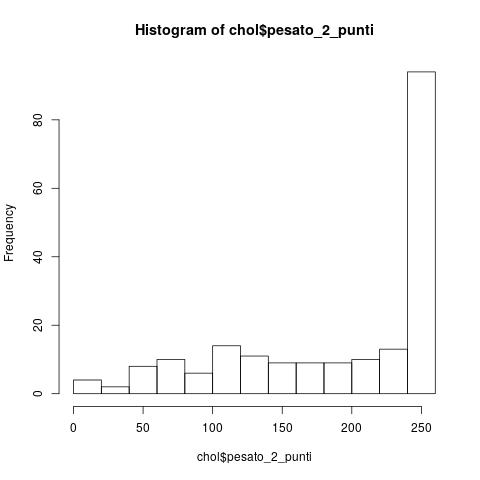
\includegraphics[width=\textwidth]{img/pesato_2_punteggio.png}
    \caption{Pesato2}
    \label{Pesato2}
   \end{subfigure}
  \begin{subfigure}[b]{0.49\textwidth}
    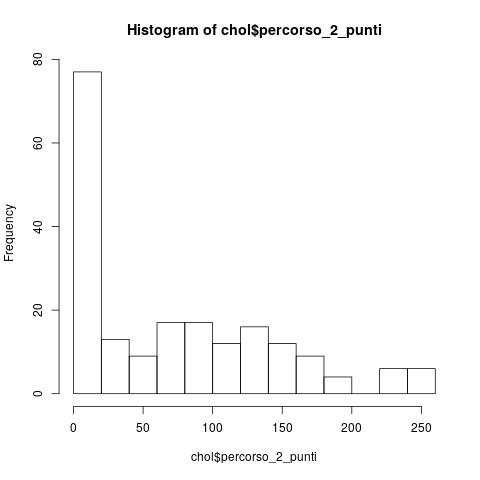
\includegraphics[width=\textwidth]{img/percorso_2_punteggio.png}
    \caption{Percorso2}
    \label{Percorso2}
  \end{subfigure}
  \caption{Istogramma del punteggio raggiunto giocando contro  i fantasmi Blinky e Pinky. La figura \ref{Pesato2} si riferisce all'agent \emph{pesato}, la \ref{Percorso2} al \emph{percorso}}
  \label{pesatoPercorso2}
\end{figure}


\subsubsection{Blinky, Pinky e Inky}

L'arrivo di Inky non sconvolge le prestazioni dell'agent \emph{percorso}. Calano le sue possibilità di completare il labirinto (in realtà in nessuna delle duecento partite giocate a $3$ fantasmi l'agent lo ha completato), ma la distribuzione dei punteggi rimane pressapoco la stessa ottenuta nelle partite con due soli fantasmi (vedi figura \ref{pesatoPercorso3}).

L'agent \emph{pesato} diversamente da \emph{percorso} è capace di completare il labirinto anche in presenza di tre fantasmi. Come si vede in figura \ref{pesatoPercorso3} l'agent ha pressapoco la stessa possibilità di vincere che quella di terminare il gioco con un punteggio all'interno di uno qualsiasi degli intervalli di campionamento. Nello specifico, l'agent ha completato il labirinto $19$ volte su $200$, cioè circa il $10\%$ delle partite.

Con la presenza di tre fantasmi è interessante notare come avviene la cattura di Pac-Man. Le partite condotte dall'agent \emph{percorso} finiscono spesso con Pac-Man intrappolato tra Blinky e Inky. Questo si spiega se si pensa agli agent che guidano i due fantasmi. Infatti, Inky è scritto per inserirsi proprio tra Pac-Man e Blinky, quindi è naturale che l'azione dei due insieme porti Pac-Man ad esaurire le vie di fuga.\\
Le cose però vanno diversamente quando è l'agent \emph{pesato} a condurre il gioco che spesso finisce con la cattura di Pac-Man da parte di Pinky.\\
Questo agent non si comporta come l'altro che reagisce alla prossimità dei fantasmi, ma al contrario pianifica il proprio percorso cercando di evitarli, o meglio pianifica il percorso più leggero, cioè quello che risulta più \emph{breve} tra il vertice su cui si trova Pac-Man e il vertice obiettivo. Per comprendere il perché della fine Pac-Man tra le grinfie di Pinky, anziché Blinky o Inky come capita con l'altro agent, dobbiamo analizzare proprio l'algoritmo A* alla base dell'agent in combinazione con lo specifico algoritmo che guida Pinky durante il gioco.

Pinky è programmato per puntare avanti quattro celle rispetto a Pac-Man e questo lo porta spesso ad essere su un percorso diverso rispetto a Blinky e Inky che invece tendono a viaggiare appaiati.\\
Si capisce che Pac-Man tende quindi a trovarsi tra due poli, uno in cui è presente Pinky e l'altro in cui sono presenti e vicini Blinky e Inky. Il loro peso viene quindi sommato e il percorso che punta verso Pinky preferito a quello che punta agli altri due fantasmi.


\begin{figure}
  \centering
  \begin{subfigure}[b]{0.49\textwidth}
    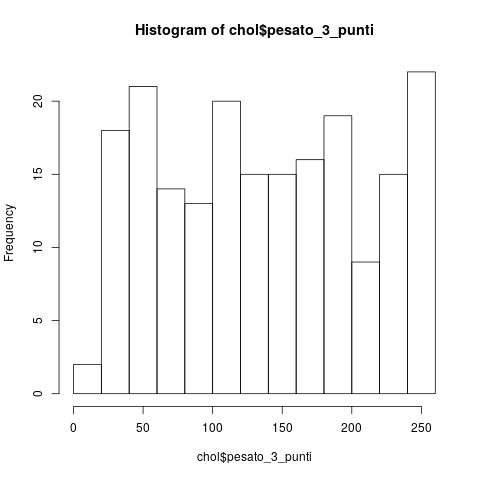
\includegraphics[width=\textwidth]{img/pesato_3_punteggio.png}
    \caption{Pesato3}
    \label{Pesato3}
   \end{subfigure}
  \begin{subfigure}[b]{0.49\textwidth}
    \includegraphics[width=\textwidth]{img/percorso_3_punteggio.png}
    \caption{Percorso3}
    \label{Percorso3}
  \end{subfigure}
  \caption{Istogramma del punteggio raggiunto giocando contro  i fantasmi Blinky, Pinky e Inky. La figura \ref{Pesato3} si riferisce all'agent \emph{pesato}, la \ref{Percorso3} al \emph{percorso}}
  \label{pesatoPercorso3}
\end{figure}


\subsubsection{Blinky, Pinky, Inky e Clyde}

Il compito di questo agent di fronte all'intero ghost team diventa superiore alle sue possibilità, infatti di $200$ partite ne vince solo una, però i suoi risultati sono nettamente migliori rispetto all'agent \emph{percorso} che praticamente finisce più della metà delle partite con un punteggio inferiore a $30$ (vedi figura \ref{pesatoPercorso4}).

\begin{figure}
  \centering
  \begin{subfigure}[b]{0.49\textwidth}
    \includegraphics[width=\textwidth]{img/pesato_4_punteggio.png}
    \caption{Pesato4}
    \label{Pesato4}
   \end{subfigure}
  \begin{subfigure}[b]{0.49\textwidth}
    \includegraphics[width=\textwidth]{img/percorso_4_punteggio.png}
    \caption{Percorso4}
    \label{Percorso4}
  \end{subfigure}
  \caption{Istogramma del punteggio raggiunto giocando contro  i fantasmi Blinky, Pinky, Inky e Clyde. La figura \ref{Pesato4} si riferisce all'agent \emph{pesato}, la \ref{Percorso4} al \emph{percorso}}
  \label{pesatoPercorso4}
\end{figure}



\section{Considerazioni}\label{tocux5f94}

La nuova implementazione della funzione per la stima euristica della distanza ha contribuito in modo evidente alle capacità di fuga di Pac-Man. Il risultato è senz'altro interessante in quanto la fuga \emph{emerge} dall'algoritmo senza essere stata specificatamente implementata.\\
Questo agent ha però ancora due limiti importanti. Il primo è che la scelta del vertice \emph{goal} è basata sulla funzione \texttt{rand} che, sebbene venga corretta in caso di cella vuota, non rappresenta comunque una scelta ragionata dell'obiettivo. Il secondo è che anche questo agent non sfrutta la conoscenza delle \emph{abitudini} dei fantasmi.\\
Questo punto merita un approfondimento. Anzi tutto vediamo che in linea di principio non è possibile definire un agent che vinca a priori se non si stabiliscono alcune regole del gioco che infatti Toru Iwatani ha saputo inserire sapientemente:

\begin{itemize}
\item
  Le pillole energetiche permettono a Pac-Man di mangiare i fantasmi
\item
  I fantasmi non possono stazionare in una cella in attesa di Pac-Man
\end{itemize}

La prima regola aiuta molto il completamento del gioco, ma la seconda è pressoché indispensabile. I vertici del grafo del labirinto di Pac-Man hanno grado massimo $4$. Considerando che i fantasmi sono $4$ è facile capire come possano organizzarsi per presidiare un vertice e quindi impedire il completamento del gioco o comunque bloccare Pac-Man in un corridoio o in un vertice. Questo ci fa capire che la fuga non può essere garantita senza il rispetto di queste regole.

Anche se i fantasmi si organizzassero in una ronda attorno ad una delle isole il gioco sarebbe irrisolvibile. Da questo segue che la vittoria sul ghost team non può essere assicurata nel labirinto del Pac-Man se non si modella l'agent di Pac-Man sull'implementazione specifica degli agent dei fantasmi.\\
Questo obiettivo può essere raggiunto sfruttando la conoscenza di detti agent che si ha a priori, in quanto si conoscono le loro regole interne, oppure programmando un agent che apprenda partita dopo partita.\\
Entrambe queste soluzioni sono però indipendenti dalla teoria dei grafi e vanno al di fuori dell'obiettivo di questo libro.

\newpage
\section*{Box domande n.6}
\addcontentsline{toc}{section}{Box domande n.6}

\begin{enumerate}
\item Cos'è il grado minimo di un grafo?

\begin{enumerate}
\def\labelenumi{\alph{enumi}.}
\item
  Il numero minimo di vertici per cui è necessario passare al fine di coprire tutti gli archi
\item
  Il numero minimo di vertici che formano un anello all'interno del grafo
\item
  Il numero minimo di archi entranti (o uscenti) da ogni vertice
\end{enumerate}

\item Perché nell'agent \texttt{percorso} non è sufficiente calcolare il percorso una volta per tutte a \emph{design-time}, ma è necessario ricalcolarlo ad ogni turno durante l'esecuzione?

\begin{enumerate}
\def\labelenumi{\alph{enumi}.}
\item
  Perché, durante il gioco, i fantasmini si muovono andando a cambiare i pesi dei possibili percorsi
\item
  Perché, durante il gioco, Pac-Man si muove cambiando le sue coordinate
\item
  Perché la funzione euristica necessita un aggiornamento continuo
\end{enumerate}

\item Qual è la differenza tra un meccanismo di fuga basato sul controllo diretto e uno basato sull'euristica pesata?

\begin{enumerate}
\def\labelenumi{\alph{enumi}.}
\item
  Il controllo diretto, quando Pac-Man si trova ad una certa distanza dal fantasma, lo fa scappare allontanandolo dal percorso che stava seguendo, mentre il controllo basato sull'euristica pesata consiste in una continua riconfigurazione del percorso che consenta di evitare i fantasmi
\item
  Il controllo diretto è l'equivalente di giocare con un JoyStick. L'agent non pianifica un percorso ma stabilisce ad ogni turno di gioco la cella su cui far spostare Pac-Man. L'agent che implementa l'euristica pesata, invece, stabilisce un percorso e lo riconfigura durante il gioco.
\item
  Il controllo diretto fa parte dell'euristica pesata. E' l'operazione con cui l'agent, prima di ricalcolare il peso del percorso, identifica le posizioni dei fantasmi
\end{enumerate}

\item
Perché Pac-Man, guidato dall'agent \texttt{percorso} ed inseguito da tre fantasmi (Blinky, Pinky e Inky), viene più facilmente mangiato da Pinky che dagli altri due?

\begin{enumerate}
\def\labelenumi{\alph{enumi}.}
\item
  Perché Pinky punta sempre alla cella che si trova 4 posizioni davanti a Pac-Man, inserendosi all'interno di un percorso per cui lui ha già calcolato il peso
\item
  Perché tra tutti i fantasmi Pinky è quello meno ``pesante''
\item
  Perché Blinky e Inky, si muovono insieme vicini e, nel caso Pac-Man si trovi a dover scegliere se dirigersi verso loro due o verso Pinky, sceglierà la direzione di Pinky, in quanto meno ``pesante''
\end{enumerate}

\end{enumerate}


\chapter{La pillola più vicina}\label{tocux5f95}

In questo capitolo ci occupiamo della scelta ragionata del vertice \emph{goal} che è l'ultimo aspetto rimasto ancora \emph{naive} dell'implementazione dell'agent di Pac-Man.

\section{Prima\ldots{} respira}

Per implementare un agent che scelga in modo \emph{intelligente} il vertice verso cui dirigersi abbiamo bisogno di un nuovo algoritmo che fa parte dell'armamentario di chi si occupa di grafi, questo è il \emph{Breadth-first search} (BFS) che, insieme all'algoritmo \emph{Depth-first search} (DFS), è un algoritmo di attraversamento e ricerca attraverso un grafo.

L'idea alla base del BFS è di ricercare all'interno di un grafo valutando prima tutti i vertici vicini al vertice di partenza (start), poi, se tra loro nessuno corrisponde al criterio di ricerca, passare al livello successivo, cioè a valutare i vertici vicini dei vicini e così via.\\
Nel nostro caso, il criterio di ricerca è la presenza di una pillola. In pratica, dato il vertice su cui si trova Pac-Man, vogliamo trovare il primo vertice che contiene una pillola, cioè non vuoto.

In figura \ref{BSF_select_1} è rappresentato Pac-Man in una regione vuota di pillole. Lo scopo è quello di dirigerlo verso la pillola più vicina. L'algoritmo BFS valuta prima i vicini prossimi al vertice di Pac-Man che sono indicati con il numero $1$, poi i vertici direttamente collegati ai suoi vicini, indicati con il numero $2$. La ricerca dell'algoritmo continua finché non viene trovato il primo vertice con una pillola.\\

\begin{figure}
  \centering
  \includegraphics[width=0.5\textwidth]{img/BSF_select_1.png}
  \caption{I vertici accessibili vicini a quello in cui si trova Pac-Man sono indicati dal numero $1$ che indica il livello di prossimità. I vicini dei vertici di livello $1$ sono indicati dal numero $2$, i vicini dei vertici di livello $2$ sono indicati con un $3$ e via dicendo. La prima pillola si trova su un vertice di livello $4$.}
  \label{BSF_select_1}
\end{figure}


Il BFS si distingue dal DFS che invece preso uno dei vicini del vertice start, continua la ricerca attraverso i vertici collegati finché non trova un vertice corrispondente al criterio di ricerca, se non lo trova, passa al prossimo vicino di livello $1$. Questo secondo approccio non è ottimale in un labirinto completamente connesso come quello di Pac-Man in quanto dato il vertice start, la ricerca attraverso il primo dei vicini di livello 1 risulterebbe sempre comunque esaustiva (figura \ref{DSF_select}).

\begin{figure}
  \centering
  \includegraphics[width=0.5\textwidth]{img/DSF_select.png}
  \caption{I vertici accessibili vicini a quello in cui si trova Pac-Man sono indicati dal numero $1$ che indica il livello di prossimità. I vicini dei vertici di livello $1$ sono indicati dal numero 2, i vicini dei vertici di livello $2$ sono indicati con un $3$ e via dicendo. La prima pillola si trova su un vertice di livello $5$.}
  \label{DSF_select}
\end{figure}


\section{Implementazione BFS}

L'implementazione dell'algoritmo che proponiamo è funzionale allo scopo dell'agent e risulta più semplice di quella normalmente proposta. Infatti useremo il BFS non per calcolare il percorso verso il primo vertice \emph{papabile} (cioè con la pillola) ma solo per conoscerne l'indice, mentre poi useremo l'algoritmo A* precedentemente sviluppato per calcolare il percorso dalla posizione corrente ad esso.

\begin{spacing}{0.9}
  \begin{small}
    \begin{tcolorbox}
\begin{verbatim}
int agri_breadthfirstsearch(int start, 
		    agri_Vertex * agri_Vertices_Colligati,
		    int (*visitatus)(int ),
		    int nmembri
		    );
\end{verbatim}
  \end{tcolorbox}
    \end{small}
      \end{spacing}

 Come si vede dal prototipo la funzione non torna un path, ma un intero che rappresenta l'indice del vertice trovato.

L'implementazione in sé stessa è molto simile a quella dell'A*.\\
Anzitutto il vertice \emph{start} viene inserito nella lista usata per implementare la coda dei vertici che sono stati valutati:

\begin{spacing}{0.9}
  \begin{small}
    \begin{tcolorbox}
\begin{verbatim}
Ordo_insero_nodus(&candidati,start,1);
\end{verbatim}
  \end{tcolorbox}
    \end{small}
      \end{spacing}
    
Il vertice viene poi estratto dalla coda e vengono ricercati tutti i suoi vicini che a loro volta vengono inseriti nella coda:

\begin{spacing}{0.9}
  \begin{small}
    \begin{tcolorbox}
\begin{verbatim}
int corrente = Ordo_pop(&candidati);

for(int i=0; i<PORTE; i++)
  {
    vicino[i] = agri_Vertices_Colligati[corrente].ianua[i];
  }

for(int i =0; i<PORTE; i++)
  {
    int iv = vicino[i];
    if(iv == -1)continue;
    precedente[iv] = corrente;
    Ordo_insero_nodus(&candidati,iv,1);
  }
\end{verbatim}
  \end{tcolorbox}
    \end{small}
      \end{spacing}
        
Per ognuno dei vicini viene quindi ripetuta la stessa procedura:

\begin{itemize}
\item
  Estrazione dalla coda
\item
  Verifica della presenza della pillola
\item
  Ricerca dei vicini con inserimento nella coda
\end{itemize}

finché la coda non risulta vuota oppure finché in uno dei vertici viene trovata la pillola.

\section{Implementazione dell'agent \emph{respiro}}

Il codice completo dell'agent che stiamo sviluppando è riportato nel listato \texttt{gioca\_tuki\_respiro.c}. La differenza fondamentale rispetto all'agent \emph{pesato} si trova nella scelta del vertice \emph{goal}.\\
Nell'agent precedente esso veniva scelto in modo pseudo-casuale

\begin{spacing}{0.9}
  \begin{small}
    \begin{tcolorbox}
\begin{verbatim}
do
  {
    vertice_goal = (double)rand()/
      ((double)RAND_MAX)*NODI_LAB_POT;
  }
 while(labx[grafo[vertice_goal].linea]
       [grafo[vertice_goal].columna]== 'J');
\end{verbatim}
  \end{tcolorbox}
    \end{small}
      \end{spacing}
  
    tra tutti i vertici del grafo, salvo poi filtrare il risultato con solo quelli in cui è presente la pillola.\\
    Nell'agent presente, invece, il punto di forza è proprio nella scelta del \emph{goal} che risulterà sempre una scelta ragionata

\begin{spacing}{0.9}
  \begin{small}
    \begin{tcolorbox}
\begin{verbatim}
vertice_goal = agri_breadthfirstsearch
  (vertice_corrente, 
   grafo,
   visitatus,
   NODI_LAB_POT
   );
\end{verbatim}
  \end{tcolorbox}
    \end{small}
      \end{spacing}

\subsection{Test dell'agent}

Una volta editato e compilato l'agent secondo la solita procedura già vista in precedenza, il primo test da condurre è quello di Pac-Man in assenza di fantasmi.

Lanciando l'eseguibile non potrà sfuggire la naturalezza con la quale Pac-Man completerà il labirinto senza scatti e interruzioni lungo il cammino.\\
Un risultato simile è stato ottenuto anche con l'agent \emph{percorso}, ma in quel caso il percorso era prestabilito a \emph{design-time} quindi era naturale che in assenza di fantasmi risultasse scorrevole.

Le sorprese arrivano quando il gioco viene lanciato con la presenza di uno o più fantasmi, infatti già in presenza di un solo fantasma vediamo che la probabilità che l'agent completi il labirinto è molto bassa nonostante si usi ancora l'algoritmo A* pesato per la pianificazione del percorso. Perché succede questo?\\
La risposta è invero piuttosto ovvia. La scelta del vertice tramite BFS comporta come prima conseguenza che una volta che Pac-Man ha imboccato un corridoio in cui sono presenti le pillole, lo completerà tutto passando iterativamente dalla posizione in cui si trova al vertice \emph{goal} corrispondente esattamente alla cella successiva a quella che sta occupando. In pratica il risultato della chiamata ad BFS è il vertice successivo a quello in cui si trova Pac-Man. Dato questo, l'uso dell'A* con la funzione euristica pesata risulta inutile finché nel percorso Pac-Man non incontra un punto di discontinuità (per esempio un corridoio già svuotato) e in questo caso l'A* ha l'opportunità di pianificare un percorso che tenda ad escludere i fantasmi.

Nel prossimo capitolo vediamo come preservare i vantaggi acquisiti con l'agent \emph{pesato} sfruttandoli insieme all'agent \emph{respiro}.

\newpage
\section*{Box domande n.7}
\addcontentsline{toc}{section}{Box domande n.7}

\begin{enumerate}
  \item
In che modo A* e BFS collaborano al raggiungimento della cella contenente la pillola più vicina

\begin{enumerate}
\def\labelenumi{\alph{enumi}.}

\item
  BFS calcola i possibili percorsi per raggiungere la cella e A* sceglie il più breve
\item
  BFS individua la cella, A* calcola il percorso più breve per raggiungerla
\item
  A* e BFS calcolano entrambi un percorso per raggiungere la cella e viene scelto il più breve
\end{enumerate}

\item
Cosa restituisce la funzione \texttt{agri\_breadthfirstsearch}?

\begin{enumerate}
\def\labelenumi{\alph{enumi}.}

\item
  L'indice della prossima cella da raggiungere
\item
  La sequenza di celle da percorrere
\item
  L'indice della prossima cella per cui passare per raggiungere la cella bersaglio
\end{enumerate}

\item
Perché l'uso di A* con l'euristica pesata risulta inutile nel percorso finché Pac-Man non si trova in una cella che non abbia pillole confinanti?

\begin{enumerate}
\def\labelenumi{\alph{enumi}.}

\item
  Perché BFS non chiama A* quando la cella obiettivo è una cella limitrofa
\item
  Perché A* considera solo il peso del percorso che calcola dalla cella di partenza alla cella obiettivo. Sa la cella obiettivo è, ad ogni turno, la cella immediatamente limitrofa, non si accorgerà se si sta dirigendo o meno in bocca a un fantasma.
\item
  Perché in presenza del BFS l'A* prevale sull'euristica pesata
\end{enumerate}
\end{enumerate}


\chapter{Il respiro\ldots{} pesato}

In questo capitolo non introduciamo nessun nuovo concetto, ma vediamo come usare l'algoritmo BFS in un modo diverso dal suo uso comune. Nel capitolo precedente lo abbiamo usato per scoprire il vertice (cioè la cella) più vicina a quella di Pac-Man con presente una pillola.\\
Come abbiamo visto in precedenza il labirinto di Pac-Man non permette un cammino euleriano e quindi in tutti i casi, anche in assenza di fantasmi, non è possibile completare il gioco senza mai \emph{staccare}, cioè senza dover ritornare lungo un percorso già esplorato. Ribadiamo questo concetto perché spiega ulteriormente il ruolo del BFS nel realizzare una partita dove Pac-Man \emph{scorre} in modo abbastanza naturale, senza eccedere nel \emph{vagabondaggio} alla ricerca di tutte le pillole.

La richiesta di \emph{scorrevolezza}, però, abbiamo visto essere in conflitto con l'esigenza di fuggire, in quanto questa comporta per forza il dover abbandonare il cammino prescelto per evitare gli attacchi dei fantasmi. Inoltre, se la fuga è basata sul calcolo del cammino pesato usando l'A*, questi non ha modo di espletare la sua funzione in quanto nella maggior parte dei casi la cella \emph{goal} è sempre quella innanzi a Pac-Man. Quindi l'algoritmo BFS e l'A* insieme, non funzionano per l'agent di Pac-Man.

\section{Ricercare i fantasmi}

Per dare qualche chance in più a Pac-Man di completare la partita è necessario che l'agent eviti gli attacchi del ghost team quando i fantasmi sono nei paraggi. All'inizio del libro, la prima soluzione che abbiamo intrapreso in questa direzione è stato il controllo delle celle vicine a quella di Pac-Man con il relativo cambio di direzione in concomitanza alla presenza di un fantasma. Come si è visto però questo approccio alla fuga funziona egregiamente quando c'è solo un fantasma, ma risulta poco efficace già quando i fantasmi sono due. Inoltre ha poco a che fare con la teoria dei grafi, per cui in ogni caso è una strategia che una volta vista non implementiamo nuovamente.

In questo paragrafo vogliamo invece implementare una nuova strategia \emph{evitante} che porti l'agent ad avere consapevolezza della presenza dei fantasmi in modo da poter attuare una strategia difensiva.

L'idea è quella di usare l'algoritmo BFS in modo alternativo, per eseguire una ricerca \emph{breath first} dei fantasmi attorno a Pac-Man.\\
A questo scopo copiamo il nostro stesso codice dalla libreria \texttt{agri} e creiamo una funzione utente basata sul principio del BFS ma con un compito più specifico: ricercare i fantasmi in prossimità di Pac-Man proseguendo la ricerca fino ad una certa profondità (o livello). Se il fantasma viene trovato, la funzione ritorna il livello a cui è stato trovato il fantasma, in modo simile ad un radar.\\
Basandoci su detto livello l'agent decide se abbandonare la ricerca delle pillole per darsi alla fuga. In pratica il livello corrisponde alla distanza del fantasma più vicino a Pac-Man il quale può stabilire la propria asticella di allarme e decidere di conseguenza (vedi figura \ref{escape_}).\\

\begin{figure}
  \centering
  \includegraphics[width=0.5\textwidth]{img/escape_.png}
  \caption{Pac-Man e il ghost team sono nel labirinto. I numeri dentro alle celle corrispondono alla distanza misurata in celle dalla posizione di Pac-Man alla cella corrispondente.}
  \label{escape_}
\end{figure}

Chiamiamo detta funzione \texttt{phantasmatis\_presentia}, il cui prototipo è analogo a quello della \texttt{agri\_breadthfirstsearch}:

\begin{spacing}{0.9}
  \begin{small}
    \begin{tcolorbox}
\begin{verbatim}
int phantasmatis_presentia(
        int start, 
        agri_Vertex * agri_Vertices_Colligati,
        int (*fantasma_presente)(int ),
        int nmembri
        )
\end{verbatim}
  \end{tcolorbox}
    \end{small}
      \end{spacing}

La \texttt{phantasmatis\_presentia} viene chiamata dall'agent fintanto che non viene individuato un vertice-cella raggiungibile attraverso un percorso sicuro:

\begin{spacing}{0.9}
  \begin{small}
    \begin{tcolorbox}
\begin{verbatim}
int tent = 0;
while(sicuro<DISTANZA_SICUREZZA)
  {
    do{
      tent++;
      vertice_goal = 
        (double)rand()/
        ((double)RAND_MAX)*NODI_LAB_POT;
    }
    while(
          labx[grafo[vertice_goal].linea]
          [grafo[vertice_goal].columna] == 'J' &&
          tent<TENTATIVI
          );
    vertice_goal = 
      evita_casa_fantasmi(vertice_goal);
    sicuro = 
      phantasmatis_presentia 
      (vertice_goal, grafo,
       phantasmatis,
       NODI_LAB_POT);
  }
\end{verbatim}
  \end{tcolorbox}
    \end{small}
      \end{spacing}

\subsection{Test e verifica}

L'agent completo che implementa la logica di fuga dai fantasmi è presentato nel listato \texttt{gioca\_tuki\_evita.c}. Dopo averlo editato e compilato secondo le modalità già presentate si può procedere alla verifica delle sue performance partendo dal gioco senza ghost team per poi aumentare gradatamente il numero di fantasmi.

Come è naturale aspettarsi, in assenza di fantasmi l'agent \emph{evita} mostra lo stesso comportamento dell'agent \emph{respiro}. Inserendo nel gioco il primo fantasma, l'agent riesce sempre a completare il labirinto continuando a mostrare un andamento \emph{scorrevole} e naturale nella scelta del percorso.\\
Con due fantasmi le difficoltà dell'agent aumentano, ma esso continua ad esibire fluidità di movimento e un alta percentuale di successo nel completamento delle partite.\\
Con tre e quattro fantasmi l'agent continua a vincere alcune partite, ma la percentuale scende significativamente. La cosa veramente notevole è che si manifesta spontaneamente un comportamento \emph{intelligente} dell'agent che sembra prevedere le mosse dei fantasmi e sganciarsi dal percorso che stava percorrendo per sfuggire loro come se fosse guidata da un essere umano o da un sistema di AI.

\subsection{Ulteriori applicazioni}

La funzione \texttt{phantasmatis\_presentia} può trovare anche un'altra applicazione nel gioco. Essa può essere usata per dirigere Pac-Man verso i fantasmini e quindi cacciarli quando sono nello stato \emph{frightened} (impaurito), cioè sono blu. Ovviamente si dovrà anche completare la gestione dello stato \emph{frightened} che in questa piattaforma non è gestito in modo completo per motivi di semplicità espositiva e di spazio.

\chapter{Conclusione}\label{tocux5f22}

In questo libro abbiamo cercato di aiutare Pac-Man a ottimizzare il suo tempo cercando di attraversare il labirinto con ``consapevolezza'' e anche sfuggendo ai fantasmi che lo inseguono da quarant'anni.\\
Abbiamo visto che l'uso di un grafo ci consente di ragionare su basi algoritmiche su questi problemi e di trovare soluzioni più efficienti. Inoltre, l'uso di grafi e algoritmi sui grafi consente di ragionare e sviluppare soluzioni indipendenti o quasi indipendenti dalla forma specifica del labirinto.\\

Le soluzioni implementate hanno lo scopo di guidare il lettore nello studio dei grafi e dei principali algoritmi con cui trattarli. La ricerca di una soluzione che garantisca al 100\% la vittoria di Pac-Man esula quindi dallo scopo di questo libro. Infatti, essendo $4$ il grado massimo del grafo, come il numero dei fantasmi, una soluzione che garantisca la vittoria richiederebbe la conoscenza da parte dell'agent della strategia dei fantasmi o, eventualmente, un algoritmo di machine learning che la apprenda.\\ 

Questa lettura ha un doppio valore. Da un lato, abbiamo incontrato alcuni concetti teorici dell'informatica e abbiamo visto come lavorare con loro e come sviluppare nuovi algoritmi. Dall'altro, come è stato detto, i problemi di Pac-Man sono in realtà anche i problemi di diversi agenti (spesso robot e droni) che devono muoversi nel mondo reale. I grafi e gli algoritmi sui grafi sono oggetto di studio crescente per la ricerca di soluzioni performanti nel campo della logistica e in altri settori produttivi e scientifici.

\part{Appendice}

\chapter[Codice MVC e fantasmi]{Appendice: Codice completo dell'MVC e dei fantasmi}

\textbf{Listato tuki\_controllo.c}
\lstinputlisting[language=C,basicstyle=\tiny]{./LIBROGRAFI/mvc/tuki5_controllo.c}

\textbf{Listato tuki\_modello.c}
\lstinputlisting[language=C,basicstyle=\tiny]{./LIBROGRAFI/mvc/tuki5_modello.c}

\textbf{Listato tuki\_modello.c}
\lstinputlisting[language=C,basicstyle=\tiny]{./LIBROGRAFI/mvc/tuki5_modello.h}

\textbf{Listato tuki\_visore.c}
\lstinputlisting[language=C,basicstyle=\tiny]{./LIBROGRAFI/mvc/tuki5_visore.c}

\textbf{Listato tuki\_visore.h}
\lstinputlisting[language=C,basicstyle=\tiny]{./LIBROGRAFI/mvc/tuki5_visore.h}

\textbf{Listato tuki\_modello.c}
\lstinputlisting[language=C,basicstyle=\tiny]{./LIBROGRAFI/ghost_team/gioca_fantasmi.c}

\chapter[Fondamenti di latino]{Appendice: Fondamenti di latino}

\section{I sostantivi}

Il latino è una lingua declinata. Questo significa che ogni sostantivo nella frase cambia in base al ruolo che svolge.\\
Ciò che cambia non è l'intera parola, ma solo la sua parte finale.

Ad esempio, consideriamo il sostantivo ``ragazza'' in queste due frasi:

\begin{enumerate}
\item
  La ragazza è bella
\item
  Ho visto la ragazza
\end{enumerate}

Nella prima frase la ragazza è il soggetto.\\
Nel secondo, la ragazza non è più il soggetto. Sono io il soggetto e lei è l'oggetto su cui ricade la mia azione (complemento oggetto).\\
Sebbene la parola ``ragazza'' svolga due ruoli diversi nelle due frasi, la parola non cambia, spetta al lettore comprendere la differenza.\\

Consideriamo ora la traduzione latina:

\begin{enumerate}
\item
  Puella pulchra est
\item
  Puellam vidi
\end{enumerate}

\emph{Puella} significa ``ragazza''.\\
Come potete vedere, nelle due frasi, la parte finale della parola è cambiata.\\
Questo è l'effetto della declinazione: a seconda del ruolo che svolge nella frase, un nome viene declinato in diversi ``casi''.

\section{I casi}\label{tocux5f56}

Esistono sei casi ciascuno dei quali rappresenta uno o più ruoli che un sostantivo può assumere:

\begin{enumerate}
\item
  Nominativo: soggetto\\
  ex. "\textbf{La ragazza} è bella" -\textgreater{} \emph{Puella pulchra est}
\item
  Genitivo: complemento di specificazione\\
  ex. "Questo è il libro \textbf{della ragazza}" -\textgreater{} \emph{Hic puellae liber est}
\item
  Dativo: complemento di termine\\
  ex. "Regalo una penna \textbf{alla ragazza}" -\textgreater{} \emph{calamum puellae dono}
\item
  Accusativo: complemento oggetto\\
  ex. "Ho visto \textbf{la ragazza}" -\textgreater{} \emph{Puellam vidi}
\item
  Vocativo: complemento di vocazione\\
  ex. "Vieni qui per favore, \textbf{ragazza}" -\textgreater{} \emph{Veni, puella}
\item
  Ablativo: altri complementi\\
  ex. "Sono andato al mare \textbf{con la ragazza}" -\textgreater{} \emph{Ab litori, cum puella ivi}
\end{enumerate}

\section{Le declinazioni}\label{tocux5f57}

Sembra abbastanza facile, giusto? A seconda del ruolo che un sostantivo svolge nella frase, cambiamo la sua fine e il gioco è fatto.\\
Sfortunatamente, non è così facile come può sembrare. In realtà non esiste un solo modo per declinare un nome nei sei casi, ma \ldots{} cinque modi diversi.\\
Ognuno di questi modi corrisponde a una declinazione.

In latino ogni nome appartiene a una declinazione.\\
Paragoniamolo con un linguaggio di programmazione orientato agli oggetti.\\
Immaginiamo che il \emph{sostantivo} sia una classe astratta con un metodo \emph{declino (caso)} non implementato che restituisce il nome declinato nel caso specificato.\\
Il latino ha cinque classi che derivano da quella classe astratta e che implementano il metodo ``\emph{declino}'' in modo diverso.

Come detto sopra, ci sono cinque declinazioni.\\
Una parola che appartiene a una specifica declinazione verrà declinata nei sei casi, seguendo le regole di tale declinazione.\\
Ad esempio, il genitivo della parola ``puella'', che appartiene alla prima declinazione, è ``puellae'', dove \textbf{ae} è la desinenza che caratterizza il genitivo di ogni parola che appartiene alla prima declinazione.

\subsection{Prima declinazione}
\begin{longtable}[c]{@{}ll@{}}
\toprule
Singolare & Plurale\tabularnewline
\midrule
\endhead
Cella & Cellae\tabularnewline
Cellae & Cellarum\tabularnewline
Cellae & Cellis\tabularnewline
Cellam & Cellas\tabularnewline
Cella & Cellae\tabularnewline
Cella & Cellis\tabularnewline
\bottomrule
\end{longtable}

\subsection{Seconda declinazione}
\begin{longtable}[c]{@{}ll@{}}
\toprule
Singolare & Plurale\tabularnewline
\midrule
\endhead
Nodus & Nodi\tabularnewline
Nodi & Nodorum\tabularnewline
Nodo & Nodis\tabularnewline
Nodum & Nodos\tabularnewline
Node & Nodi\tabularnewline
Nodi & Nodis\tabularnewline
\bottomrule
\end{longtable}

\subsection{Terza declinazione}
\begin{longtable}[c]{@{}ll@{}}
\toprule
Singolare & Plurale\tabularnewline
\midrule
\endhead
Colligatio & Colligationes\tabularnewline
Colligationis & Colligationum\tabularnewline
Colligationi & Colligationibus\tabularnewline
Colligationem & Colligationes\tabularnewline
Colligatio & Colligationes\tabularnewline
Colligatione & Colligationibus\tabularnewline
\bottomrule
\end{longtable}

\subsection{Quarta declinazione}
\begin{longtable}[c]{@{}ll@{}}
\toprule
Singolare & Plurale\tabularnewline
\midrule
\endhead
Manus & Manus\tabularnewline
Manus & Manuum\tabularnewline
Manui & Manibus\tabularnewline
Manum & Manus\tabularnewline
Manus & Manus\tabularnewline
Manu & Manibus\tabularnewline
\bottomrule
\end{longtable}

\subsection{Quinta declinazione}
\begin{longtable}[c]{@{}ll@{}}
\toprule
Singolare & Plurale\tabularnewline
\midrule
\endhead
Res & Res\tabularnewline
Rei & Rerum\tabularnewline
Rei & Rebus\tabularnewline
Rem & Res\tabularnewline
Res & Res\tabularnewline
Re & Rebus\tabularnewline
\bottomrule
\end{longtable}

\subsection{Gli elementi della libreria}

La parola \emph{ager} in Latino significa `campo', nel senso di campo di fiori o campo di grano. Ager appartiene alla terza declinazione quindi, come avrete imparato, \emph{agri} significa `del campo'.

\begin{spacing}{0.9}
  \begin{small}
    \begin{tcolorbox}
\begin{verbatim}
typedef enum {SX,DEORSUM,DX,SURSUM,FIXUS} versus
\end{verbatim}
  \end{tcolorbox}
    \end{small}
      \end{spacing}

\begin{itemize}

\item
  \textbf{versus} decl. 4: direzione
\item
  \textbf{sx} sta per sinistra decl. 1: sinistra
\item
  \textbf{deorsum} avverbio: giu
\item
  \textbf{dx} sta per dextra decl. 1: destra
\item
  \textbf{sursum} avv: su
\item
  \textbf{fixo} aggettivo: fermo
\end{itemize}

\begin{spacing}{0.9}
  \begin{small}
    \begin{tcolorbox}
\begin{verbatim}
enum genus {MURO,ALTRO}
\end{verbatim}
  \end{tcolorbox}
    \end{small}
      \end{spacing}

\begin{itemize}

\item
  \textbf{genus} decl. 3: tipo
\item
  \textbf{muro} (Italiano)
\item
  \textbf{altro} (Italiano)
\end{itemize}

\begin{spacing}{0.9}
  \begin{small}
    \begin{tcolorbox}
\begin{verbatim}
typedef enum genus rei_genus
\end{verbatim}
  \end{tcolorbox}
    \end{small}
      \end{spacing}

\begin{itemize}

\item
  \textbf{rei\_genus}: tipo dell'oggetto
\end{itemize}

\subsubsection{Grafo come una lista di archi:}\label{graph-as-a-list-of-edges}

\begin{spacing}{0.9}
  \begin{small}
    \begin{tcolorbox}
\begin{verbatim}
typedef struct {
  int linea; int columna;
  int index;
  int ianua[PORTE];
} agri_Vertex;
\end{verbatim}
  \end{tcolorbox}
    \end{small}
      \end{spacing}

\begin{itemize}

\item
  \textbf{vertex} decl. 3: vertice
\item
  \textbf{linea} decl. 1: riga
\item
  \textbf{columna} decl. 1: colonna
\item
  \textbf{index} decl. 3: indice
\item
  \textbf{ianua} decl. 1: porta
\end{itemize}

\begin{spacing}{0.9}
  \begin{small}
    \begin{tcolorbox}
\begin{verbatim}
typedef struct colligatio {
  agri_Vertex ab, ad;
  versus discessus, meta;
  int longitudo;
} agri_Colligatio;
\end{verbatim}
  \end{tcolorbox}
    \end{small}
      \end{spacing}

\begin{itemize}

\item
  \textbf{colligatio} decl. 3: arco
\item
  \textbf{discessus} decl. 4: partenza
\item
  \textbf{meta} decl. 1: destinazione
\item
  \textbf{longitudo} decl. 3: lunghezza
\end{itemize}

\begin{spacing}{0.9}
  \begin{small}
    \begin{tcolorbox}
\begin{verbatim}
typedef struct membrum {
  agri_Colligatio colligatio;
  struct membrum * next;
} agri_Membrum;
\end{verbatim}
  \end{tcolorbox}
    \end{small}
      \end{spacing}

\begin{itemize}

\item
  \textbf{colligatio} decl. 3: arco
\item
  \textbf{membrum} decl. 2: elemento
\end{itemize}

\begin{spacing}{0.9}
  \begin{small}
    \begin{tcolorbox}
\begin{verbatim}
typedef agri_Membrum * agri_Colligationes_Colligatae;
\end{verbatim}
  \end{tcolorbox}
    \end{small}
      \end{spacing}

\begin{itemize}

\item
  \textbf{colligationes colligatae}: archi connessi
\end{itemize}

\begin{spacing}{0.9}
  \begin{small}
    \begin{tcolorbox}
\begin{verbatim}
void agri_Colligationem_insero
\end{verbatim}
  \end{tcolorbox}
    \end{small}
      \end{spacing}

\begin{itemize}

\item
  \textbf{colligationem insero}: inserisco arco
\end{itemize}

\begin{spacing}{0.9}
  \begin{small}
    \begin{tcolorbox}
\begin{verbatim}
int agri_Verticem_quaero
\end{verbatim}
  \end{tcolorbox}
    \end{small}
      \end{spacing}

\begin{itemize}

\item
  \textbf{verticem quaero}: cerco un vertice
\end{itemize}

\subsubsection{Grafo come lista di vertici:}\label{graph-as-a-list-of-vertices}

\begin{spacing}{0.9}
  \begin{small}
    \begin{tcolorbox}
\begin{verbatim}
typedef agri_Vertex * agri_Verticum_Dispositio;
\end{verbatim}
  \end{tcolorbox}
    \end{small}
      \end{spacing}

\begin{itemize}

\item
  \textbf{verticum dispositio}: array di vertici
\end{itemize}

\begin{spacing}{0.9}
  \begin{small}
    \begin{tcolorbox}
\begin{verbatim}
agri_Vertex agri_Verticem_creo (
  int index, int linea, int columna);
\end{verbatim}
  \end{tcolorbox}
    \end{small}
      \end{spacing}

\begin{itemize}

\item
  \textbf{verticem creo}: creo un vertice
\end{itemize}

\begin{spacing}{0.9}
  \begin{small}
    \begin{tcolorbox}
\begin{verbatim}
typedef struct nodus_coda {
  int index;
  double prio;
  struct nodus_coda * post;
} Nodus;
\end{verbatim}
  \end{tcolorbox}
    \end{small}
      \end{spacing}

\begin{itemize}

\item
  \textbf{nodus} decl.2: nodo (elemento della coda)
\item
  \textbf{index} decl. 3: indice
\item
  \textbf{prio} sta per priorsum avv: priorità
\item
  \textbf{coda} decl.1: coda
\end{itemize}

\begin{spacing}{0.9}
  \begin{small}
    \begin{tcolorbox}
\begin{verbatim}
typedef Nodus * Ordo;
\end{verbatim}
  \end{tcolorbox}
    \end{small}
      \end{spacing}

\begin{itemize}

\item
  \textbf{ordo} decl.3: lista
\end{itemize}

\begin{spacing}{0.9}
  \begin{small}
    \begin{tcolorbox}
\begin{verbatim}
typedef int * agri_Via;
\end{verbatim}
  \end{tcolorbox}
    \end{small}
      \end{spacing}

\begin{itemize}

\item
  \textbf{via} decl.1: via, cammino
\end{itemize}

\begin{spacing}{0.9}
  \begin{small}
    \begin{tcolorbox}
\begin{verbatim}
void Ordo_amoveo_nodus(Ordo * l, int index);
\end{verbatim}
  \end{tcolorbox}
    \end{small}
      \end{spacing}

\begin{itemize}

\item
  \textbf{amoveo nodus}: rimuovo nodo
\end{itemize}

\begin{spacing}{0.9}
  \begin{small}
    \begin{tcolorbox}
\begin{verbatim}
void Ordo_insero_nodus(Ordo * l,int index,
  double prio);
\end{verbatim}
  \end{tcolorbox}
    \end{small}
      \end{spacing}

\begin{itemize}
\item
  \textbf{insero nodus}: inserisco nodo
\end{itemize}

\begin{spacing}{0.9}
  \begin{small}
    \begin{tcolorbox}
\begin{verbatim}
int Ordo_pop(Ordo * pOrdo);
\end{verbatim}
  \end{tcolorbox}
    \end{small}
      \end{spacing}

\begin{itemize}

\item
  (Inglese) pop dell'elemento in testa alla lista
\end{itemize}

\begin{spacing}{0.9}
  \begin{small}
    \begin{tcolorbox}
\begin{verbatim}
agri_Via agri_astar(
  int start, int goal,
  agri_Vertex * agri_Vertices_Colligati,
  double (*spatium)(int ab, int ad),
  double (*euristica)(int ab, int ad));
\end{verbatim}
  \end{tcolorbox}
    \end{small}
      \end{spacing}

\begin{itemize}

\item
  (Inglese) algoritmo Astar
\end{itemize}

\begin{spacing}{0.9}
  \begin{small}
    \begin{tcolorbox}
\begin{verbatim}
int index_nodus_cella(int riga, int col,
		      agri_Vertex * av);
\end{verbatim}
  \end{tcolorbox}
    \end{small}
      \end{spacing}

\begin{itemize}

\item
  \textbf{index nudus cella}: indice nodo cella
\end{itemize}

\subsubsection{Grafo come una lista di celle:}

\begin{spacing}{0.9}
  \begin{small}
    \begin{tcolorbox}
\begin{verbatim}
typedef struct dato {
  int visitata; rei_genus rei;
} Attributi;
\end{verbatim}
  \end{tcolorbox}
    \end{small}
      \end{spacing}

\begin{itemize}

\item
  \textbf{Attributi} part. perf.: attributi
\item
  \textbf{visitata} agg: visitata
\end{itemize}

\begin{spacing}{0.9}
  \begin{small}
    \begin{tcolorbox}
\begin{verbatim}
typedef struct cella {
  Attributi d;
  struct cella* dextra;
  struct cella* deorsum;
  struct cella* sinistra;
  struct cella* sursum;
} agri_Cella;
\end{verbatim}
  \end{tcolorbox}
    \end{small}
      \end{spacing}

\begin{itemize}

\item
  \textbf{Cella} decl.1: cella
\end{itemize}

\begin{spacing}{0.9}
  \begin{small}
    \begin{tcolorbox}
\begin{verbatim}
typedef agri_Cella* agri_Tabella;
\end{verbatim}
  \end{tcolorbox}
    \end{small}
      \end{spacing}

\begin{itemize}
\item
  \textbf{tabella} decl.1: tabella, griglia
\end{itemize}

\begin{spacing}{0.9}
  \begin{small}
    \begin{tcolorbox}
\begin{verbatim}
typedef struct nodo {
  agri_Cella * locus;
  struct nodo * next;
  struct nodo * prev;
} agri_Passo;
\end{verbatim}
  \end{tcolorbox}
    \end{small}
      \end{spacing}

\begin{itemize}

\item
  \textbf{passo} da passus decl.2: passo
\item
  \textbf{locus} decl.2: luogo, posizione
\end{itemize}

\begin{spacing}{0.9}
  \begin{small}
    \begin{tcolorbox}
\begin{verbatim}
typedef agri_Passo* agri_Iter;
\end{verbatim}
  \end{tcolorbox}
    \end{small}
      \end{spacing}

\begin{itemize}

\item
  \textbf{iter} decl.3: percorso
\end{itemize}

\begin{spacing}{0.9}
  \begin{small}
    \begin{tcolorbox}
\begin{verbatim}
void agri_creo_Tabellam(agri_Tabella* g);
\end{verbatim}
  \end{tcolorbox}
    \end{small}
      \end{spacing}

\begin{itemize}
\item
  \textbf{creo tabellam}: creo tabella
\end{itemize}

\begin{spacing}{0.9}
  \begin{small}
    \begin{tcolorbox}
\begin{verbatim}
agri_Tabella agri_addo_Tabellam(
  agri_Tabella tabella,Attributi d,versus dir);
\end{verbatim}
  \end{tcolorbox}
    \end{small}
      \end{spacing}

\begin{itemize}

\item
  \textbf{addo tabellam}: aggiungo tabella
\end{itemize}

\begin{spacing}{0.9}
  \begin{small}
    \begin{tcolorbox}
\begin{verbatim}
void agri_colligo_Cellas(
  agri_Cella * da, agri_Cella * a, versus da_a);
\end{verbatim}
  \end{tcolorbox}
    \end{small}
      \end{spacing}

\begin{itemize}

\item
  \textbf{colligo cellas}: connetto celle
\end{itemize}

\begin{spacing}{0.9}
  \begin{small}
    \begin{tcolorbox}
\begin{verbatim}
void agri_creo_Iter(agri_Iter* p_camm);
\end{verbatim}
  \end{tcolorbox}
    \end{small}
      \end{spacing}

\begin{itemize}

\item
  \textbf{creo iter}: creo percorso
\end{itemize}

\begin{spacing}{0.9}
  \begin{small}
    \begin{tcolorbox}
\begin{verbatim}
void agri_addo_Iter(agri_Iter * p_camm,
  agri_Cella * p_cella);
\end{verbatim}
  \end{tcolorbox}
    \end{small}
      \end{spacing}

\begin{itemize}
\item
  \textbf{addo iter}: aggiungo percorso
\end{itemize}

\begin{spacing}{0.9}
  \begin{small}
    \begin{tcolorbox}
\begin{verbatim}
agri_Cella* agri_rivela_Cella(agri_Iter ap,
  versus ricerca);
\end{verbatim}
  \end{tcolorbox}
    \end{small}
      \end{spacing}

\begin{itemize}

\item
  \textbf{rivela cella}: rivela cella
\end{itemize}

\begin{spacing}{0.9}
  \begin{small}
    \begin{tcolorbox}
\begin{verbatim}
int agri_muto(
  agri_Colligationes_Colligatae ge,
  agri_Verticum_Dispositio *a);
\end{verbatim}
  \end{tcolorbox}
    \end{small}
      \end{spacing}

\begin{itemize}
\item
  \textbf{muto}: trasformo
\end{itemize}

\begin{spacing}{0.9}
  \begin{small}
    \begin{tcolorbox}
\begin{verbatim}
int agri_dispono(
  agri_Colligationes_Colligatae list,
  agri_Colligationes_Colligatae * array);
\end{verbatim}
  \end{tcolorbox}
    \end{small}
      \end{spacing}

\begin{itemize}
\item
  \textbf{dispono}: dispongo
\end{itemize}

\begin{spacing}{0.9}
  \begin{small}
    \begin{tcolorbox}
\begin{verbatim}
int Verticem_quaero(
  agri_Verticum_Dispositio v, int index, int amplitudo);
\end{verbatim}
  \end{tcolorbox}
    \end{small}
      \end{spacing}

\begin{itemize}
\item
  \textbf{verticem quaero}: cerco un vertice
\end{itemize}

\begin{spacing}{0.9}
  \begin{small}
    \begin{tcolorbox}
\begin{verbatim}
versus agri_Versum_inverto(versus v);
\end{verbatim}
  \end{tcolorbox}
    \end{small}
      \end{spacing}

\begin{itemize}
\item
  \textbf{versum inverto}: inverto direzione
\end{itemize}

\begin{spacing}{0.9}
  \begin{small}
    \begin{tcolorbox}
\begin{verbatim}
int compar(const void * a, const void * b);
\end{verbatim}
  \end{tcolorbox}
    \end{small}
      \end{spacing}

\begin{itemize}
\item
  \textbf{compar} sta per comparo: confronto
\end{itemize}

%%%%%%%%%%%%%%%%%%%%%%%%%%%%%%%%%%%%%%%%%%%%%%%%%%%%%%%%%%%%%%%%%

\chapter[Codice libreria AGRI]{Appendice: Codice completo libreria AGRI}
\textbf{Listato libagri.h}
\lstinputlisting[language=C,basicstyle=\tiny]{./LIBROGRAFI/agri/lib/include/libagri.h}

\textbf{Listato libagri.c}
\lstinputlisting[language=C,basicstyle=\tiny]{./LIBROGRAFI/agri/lib/src/libagri.c}

%%%%%%%%%%%%%%%%%%%%%%%%%%%%%%%%%%%%%%%%%%%%%%%%%%%%%%%%%%%%%%%%%

\chapter[Codice agents di Pac-Man]{Appendice: Codice completo agents di Pac-Man}
\textbf{Listato gioca\_tuki\_vuoto.c}
\lstinputlisting[language=C,basicstyle=\tiny]{./LIBROGRAFI/PacMan/gioca_tuki_vuoto.c}

\textbf{Listato gioca\_tuki\_random.c}
\lstinputlisting[language=C,basicstyle=\tiny]{./LIBROGRAFI/PacMan/gioca_tuki_random.c}

\textbf{Listato gioca\_tuki\_boustrophedon.c}
\lstinputlisting[language=C,basicstyle=\tiny]{./LIBROGRAFI/PacMan/gioca_tuki_boustrophedon.c}

\textbf{Listato gioca\_tuki\_esploraeritorna.c}
\lstinputlisting[language=C,basicstyle=\tiny]{./LIBROGRAFI/PacMan/gioca_tuki_esploraeritorna.c}

\textbf{Listato gioca\_tuki\_generagrafo.c}
\lstinputlisting[language=C,basicstyle=\tiny]{./LIBROGRAFI/PacMan/gioca_tuki_generagrafo.c}

\textbf{Listato gioca\_tuki\_percorso.c}
\lstinputlisting[language=C,basicstyle=\tiny]{./LIBROGRAFI/PacMan/gioca_tuki_percorso.c}

\textbf{Listato gioca\_tuki\_pesato.c}
\lstinputlisting[language=C,basicstyle=\tiny]{./LIBROGRAFI/PacMan/gioca_tuki_pesato.c}

\textbf{Listato gioca\_tuki\_respiro.c}
\lstinputlisting[language=C,basicstyle=\tiny]{./LIBROGRAFI/PacMan/gioca_tuki_respiro.c}

\textbf{Listato gioca\_tuki\_evita.c}
\lstinputlisting[language=C,basicstyle=\tiny]{./LIBROGRAFI/PacMan/gioca_tuki_evita.c}

%%%%%%%%%%%%%%%%%%%%%%%%%%%%%%%%%%%%%%%%%%%%%%%%%%%%%%%%%%%%%%%%%

\chapter[Codice tool A*]{Appendice: Codice completo tool A*}

\lstinputlisting[language=C,basicstyle=\tiny]{./LIBROGRAFI/PacMan/test_star.c}

%%%%%%%%%%%%%%%%%%%%%%%%%%%%%%%%%%%%%%%%%%%%%%%%%%%%%%%%%%%%%%%%%

\chapter{Soluzioni}

\paragraph{Box domande n.1}\label{box-domande-n.1}

\begin{enumerate}
\item
  a
\item
  c
\item
  a
\end{enumerate}

\paragraph{Box domande n.2}\label{box-domande-n.2}

\begin{enumerate}
\item
  b
\item
  a
\item
  c
\end{enumerate}

\paragraph{Box domande n.3}\label{box-domande-n.3}

\begin{enumerate}
\item
  b
\item
  a\\
  \includegraphics[width=0.40000\textwidth]{img/num_VerticiArchi_es_sol1.png}
\item
  c\\
  \includegraphics[width=0.40000\textwidth]{img/num_VerticiArchi_es_sol2.png}
\item
  a
\end{enumerate}

\paragraph{Box domande n.4}\label{box-domande-n.4}

\begin{enumerate}
\item
  b
\item
  c
\item
  a
\end{enumerate}

\paragraph{Box domande n.5}\label{box-domande-n.5}

\begin{enumerate}
\item
  a
\item
  a
\item
  a
\end{enumerate}

\paragraph{Box domande n.6}\label{box-domande-n.6}

\begin{enumerate}
\item
  c
\item
  a
\item
  a
\item
  c
\end{enumerate}

\paragraph{Box domande n.7}\label{box-domande-n.7}

\begin{enumerate}
\item
  b
\item
  a
\item
  b
\end{enumerate}


\begin{thebibliography}{9}

\bibitem[Zachary]{Zachary}
https://en.wikipedia.org/wiki/Zachary's\_karate\_club
\bibitem[Rohlfshagen]{Rohlfshagen}
  Pac-Man Conquers Academia: Two Decades of Research Using a Classic Arcade Game,IEEE TRANSACTIONS ON GAMES, VOL. 10, NO. 3, SEPTEMBER 2018
\bibitem{}
  Algorithm of ghost behavior in the game Pac-Man: \\https://weekly-geekly.github.io/articles/109406/index.html
\bibitem[Williams]{Williams}
   P. R. Williams, D. Perez-Liebana and S. M. Lucas, "Ms. Pac-Man Versus Ghost Team CIG 2016 competition," 2016 IEEE Conference on Computational Intelligence and Games (CIG), Santorini, 2016, pp. 1-8, doi: 10.1109/CIG.2016.7860446.
\bibitem[igraph]{igraph}
Gábor Csárdi, Tamás Nepusz: The igraph software package for complex network research. InterJournal Complex Systems, 1695, 2006. 
\bibitem[Bahnemann]{Bahnemann}
  Rik Bähnemann, Nicholas Lawrance, Jen Jen Chung, Michael Pantic, Roland Siegwart, Juan Nieto:
Revisiting Boustrophedon Coverage Path Planning as a Generalized Traveling Salesman Problem. arXiv:1907.09224
\bibitem[Choset]{Choset}
  Choset H., Pignon P. (1998) Coverage Path Planning: The Boustrophedon Cellular Decomposition. In: Zelinsky A. (eds) Field and Service Robotics. Springer, London
\bibitem[Brooks]{Brooks}
Rodney A.Brooks (1991): 
Intelligence without representation: MIT Artificial Intelligence Laboratory, 545 Technology Square, Rm. 836, Cambridge, MA 02139, USA

\bibitem[toruIwatani]{toruIwatani}
  figura \ref{toruIwatani}\\
  Official GDC, CC BY 2.0\\
  <https://creativecommons.org/licenses/by/2.0>,\\
  via Wikimedia Commons

\bibitem[cartuccia]{cartuccia}
  figura \ref{cartuccia}\\
  Hedning, CC BY-SA 3.0\\
  <https://creativecommons.org/licenses/by-sa/3.0>,\\
  via Wikimedia Commons

\bibitem[postazione]{postazione}
  figura \ref{postazione}\\
  Peter Handke, CC0, via Wikimedia Commons

\bibitem[postazioni]{postazioni}
  figura \ref{postazioni}\\
  Marica Massaro, CC BY-SA 4.0\\
  <https://creativecommons.org/licenses/by-sa/4.0>,\\
  via Wikimedia Commons
  
\end{thebibliography}

\end{document}
